\documentclass[phd,tocprelim]{cornell}
%
% tocprelim option must be included to put the roman numeral pages\ in the
% table of contents
%
% The cornellheadings option will make headings completely consistent with
% guidelines.
%
% This template was originally provided by Blake Jacquot, and
% fixed up by Andrew Myers.
%
%Some possible packages to include
\usepackage[utf8]{inputenc}
\usepackage{graphicx,pstricks}
\usepackage{microtype}
\usepackage{graphics}
\usepackage{moreverb}
\usepackage{subfigure}
\usepackage{longtable}
\usepackage{epsfig}
\usepackage{subfigure}
\usepackage{hangcaption}
\usepackage{txfonts}
\def\Plus{\texttt{+}}
\usepackage{multirow}

\newcommand\blfootnote[1]{%
  \begingroup
  \renewcommand\thefootnote{}\footnote{#1}%
  \addtocounter{footnote}{-1}%
  \endgroup
}

%
\usepackage[
    backend=bibtex, 
    style=chicago-authordate,
    sorting=none
]{biblatex}

\addbibresource{bibliography.bib}
\usepackage{palatino}

% Packages added by Xihe:
\usepackage{subfiles}
\usepackage{bm}
\usepackage{array} % for flexible tables
\usepackage{hyperref} % for links
\usepackage{amsbsy} % for bold
\usepackage[justification=centerlast,font=small, labelfont=bf]{caption} % Figure captioning
\usepackage{indentfirst} % indent first paragraph after \section tags
\usepackage{booktabs} % for tables
\usepackage[all]{nowidow} % for widow and orphan sentences
% For multi-page figures and captions:
\DeclareCaptionLabelFormat{adja-page}{\hrulefill\\#1 #2 \emph{(Continued)}}

% DELETE THIS, ONLY ADDED FOR FILLER TEXT IN TEMPLATE
\usepackage{lipsum}

%if you're having problems with overfull boxes, you may need to increase
%the tolerance to 9999
\tolerance=9999

%\bibliographystyle{unsrt}
%\bibliographystyle{IEEEbib}

% Use hangcaption to modify indentations of figure captions
\renewcommand{\caption}[1]{\singlespacing\hangcaption{#1}\normalspacing}
\renewcommand{\topfraction}{0.85}
\renewcommand{\textfraction}{0.1}
\renewcommand{\floatpagefraction}{0.75}


\title {Understanding and predicting motor recovery after stroke: a multimodal connectomic approach}
\author {Emily Olafson}
\conferraldate {May}{2023}
\degreefield {Ph.D.}
\copyrightholder{Emily Olafson}
\copyrightyear{2023}

\begin{document}

\maketitle
\makecopyright

\begin{abstract}


Your abstract goes here. Make sure it sits inside the brackets. If not,
your biosketch page may not be roman numeral iii, as required by the
graduate school.
The abstract should state the problem, describe the methods and procedures used, and give the main results or conclusions of the research.
The abstract must not exceed 350 words in length (generally about one-and-one-half correctly spaced pages; the abstract may not be more than two pages).
\end{abstract}

\begin{biosketch}
Emily was born in Northhampton, United Kingdom in 1997, and grew up in Toronto, Canada.  In highschool, her interest in biology was nurtured  by an exceptional biology teacher.  In her first year at McGill University in Montreal, she was excited by the interdisciplinary nature of the Neuroscience major program, and ultimately joined the Honors stream where she would be able to pursue a full-year undergraduate thesis. 
In her second year, she worked in the lab of Dr. Artur Kania where she was able to apply cutting-edge technologies like CRISPR-Cas9 to modify the genome of chick embryos and analyze changes in spinal cord formation. 

 Wanting to explore computational neuroscience, she reached out to Mallar Chakravarty and joined his lab at the Douglas Mental Health University Institute processing T1w scans from individuals with autism spectrum disorder through MAGeT-Brain, a subcortical segmentation algorithm.  Her interest in human neuroimaging skyrocketed after she took a master's course in neuroimaging taught by Mallar. This course taught her how to critically engage with literature,  how to articulate complex ideas, and ultimately pushed her to apply to graduate school.

She applied to neuroscience programs across the US and ultimately ended up at Weill Cornell Graduate School in New York City.  She rotated with Amy Kuceyeski, exploring the relationship between structural and functional connectivity after stroke, and with Sudhin Shah,  investigating neural correlates of consciousness in a minimally conscious patient. Although COVID prevented her from rotating with other labs, she had already decided on joining Amy's lab, and moved to Ithaca in August 2020. 

In Amy Kuceyeski's lab,  she did a variety of things.

She taught 2 semesters in the Cornell Prison Education Program: first at Five Points Correctional Facility, and then at Cayuga Correctional Facility. She generated material for the course "Neurochemistry of Human Behavior" and taught incarcerated people about synaptic transmission, long term potentiation,  and mechanisms of disease. 

She did an internship at Biogen in their clinical imaging group.

\end{biosketch}

\begin{dedication}
\textit{To my parents, I dedicate this dissertation with my deepest gratitude. }

\end{dedication}

\begin{acknowledgements}
Thank you to Amy Kuceyeski, my mentor at Weill. Aside from your  scientific brilliance, your compassionate and trusting leadership was invaluable to me throughout my thesis, but especially during the pandemic.  You consciously create an environment in which people can  thrive. You rock. I am deeply appreciative of my thesis committee: Dr. Conor Liston, Dr. Nicholas Schiff, and Dr. Aaron Boes, for their support and expertise, both academically and professionally.

I would also like to thank the people who made Ithaca feel like home:  Parker Singleton, Ceren Tozlu, Keith Jamison, Zijin Gu, Ben, and Liam.

Thank you to mentors along the way: Mallar Chakravarty, Elvisha Dhamala, Gabriel Devenyi, Saashi Bedford, Raihaan Patel,  Elisa Guma, Artur Kania,  Daniel Morales, Sylvie Lahaie, Alyssa Dai,  Jonathan DuBois,  and Cindy Law.

To others who have made difficult experiences easier: Clive Liew, Mert Sabuncu, Randi Silver, Rebekah Ciribassi, thank you.

Thank you to my world-class friends who remind me that people are fundamentally good: Emma, Miriam, Mikey, Zoe, Nilasha, Jonah, CEC, Jasmine, Max, Board Games Club, and my Neuro entire cohort.

To the students and staff of the Cornell Prison Education Program: teaching at Five Points and Cayuga was the best thing I've ever done. From the bottom of my heart, thank you for the opportunity.

To my parents, thank you for the sacrifices you’ve made to
give me a stellar education. Thank you to my twin brother Matt, for being a lifelong best friend.

Finally, one last thank you is reserved for my partner, Isaac,  for answering all my statistics questions, for eating expensive sushi with me, and for generally being the light of my life.
\end{acknowledgements}

\contentspage
\tablelistpage
\figurelistpage

\normalspacing \setcounter{page}{1} \pagenumbering{arabic}
\pagestyle{cornell} \addtolength{\parskip}{0.5\baselineskip}

% Use subfiles for chapters for better organization
% Add labels to each chapter so you can reference them in your text with \ref{}
\chapter{Functional connectome reorganization relates to post-stroke motor recovery and structural and functional disconnection*}
\blfootnote{* Olafson, E. R., Jamison, K. W., Sweeney, E. M., Liu, H., Wang, D., Bruss, J. E., Boes, A. D., and Kuceyeski, A. (2021). Functional connectome reorganization relates to post-stroke motor recovery and structural and functional disconnection. NeuroImage, 245, 118642.}

%\subfile{../chapter1/introduction}
\section{Introduction}
Motor deficits are among the most common and disruptive symptoms of ischemic stroke. Spontaneous recovery of motor function occurs for most patients (\cite{Duncan2000-uj}), and largely depends on the ability of brain networks to functionally reorganize and compensate for lost function (\cite{Grefkes2008-bt, Rehme2013-ap}). As demonstrated by animal models, the functionality of damaged motor regions may be remapped to surviving tissue around the lesion (\cite{Winship2009-af}). However, brain areas distant to the lesion that have similar function and/or connectivity as the damaged area have also been shown to compensate for lost function (\cite{Winship2009-af, Adam2020-jk, Murata2015-ss, Brown2009-jn}).
	
	In humans, functional reorganization has been studied with functional magnetic resonance imaging (fMRI). Task fMRI studies have demonstrated that cortical reorganization related to motor recovery can be characterized by task-based activation of surviving ipsilesional cortex, contralesional areas, and even regions not classically activated by motor tasks in healthy subjects (\cite{Ward2003-zd}). Recently, resting-state fMRI has emerged as a means to study connectivity changes after stroke in subjects who are severely impaired and cannot perform motor tasks. Resting-state fMRI has been used to identify recovery-related changes in functional connectivity between specific brain regions, reflecting network-level changes (\cite{Park2011-kx}). However, few studies to date have attempted to capture longitudinal network-level reorganization after stroke using resting-state fMRI. 
	
	Prior studies investigating neural correlates of motor recovery have also focused almost exclusively on supratentorial strokes that impact the internal capsule and surrounding areas.  Infratentorial pontine strokes may impact the corticospinal tract directly or the connections between motor cortex and the cerebellum (\cite{Lu2011-ow}). These strokes  account for roughly 7 percent of all ischemic strokes (\cite{Saia2009-ik}), and may have different mechanisms of recovery-related reorganization from those of more well-studied supratentorial strokes.
	
    Remote brain areas anatomically connected to the lesion undergo structural and functional changes through a process known as diaschisis (\cite{Carrera2014-ah}). Functional remapping of areas structurally disconnected by the lesion may be an important component of the recovery process that has not been deeply explored. Recent studies have also demonstrated that functional connectivity (FC) changes occur following structural connectivity disruption after stroke (\cite{Lu2011-ow, Griffis2020-hx}). We hypothesize that functional reorganization may also occur in areas whose FC is reduced due to the stroke. In this study, we propose a novel measure to capture adaptive functional network reorganization after pontine stroke, outlined below, and relate it to patterns of regional stroke-related structural connectome disruption and measures of upper-arm motor recovery. 

	Connectivity to the rest of the brain is one aspect of a brain region's functional role in the network. We propose that instances of functional reorganization over time may be captured by identifying brain regions whose pattern of FC with the rest of the brain is more closely matched by a different brain region at a later date. Considering functional connectomes as a graph, the task of identifying similar nodes (gray matter regions, in this case) between two functional connectomes can be considered a graph matching problem (\cite{Conte2004-ro}). Conceptually, the process of graph matching exchanges the labels of regions in a network when doing so results in increased similarity of the two networks. When two regions exchange FC profiles, the regions are said to have been ‘remapped’. We hypothesize that graph matching, applied recently to brain networks for the first time to assess the relationship between functional and structural connectivity networks (\cite{Osmanlioglu2019-ao}), will allow accurate quantification of whole brain, network-level, recovery-relevant functional reorganization after stroke. 	
	
	As far as we know, no work has attempted to detect connectivity network-level functional reorganization in post-stroke recovery with longitudinal MRI, much less correlate it with measures of recovery or patterns of structural connectome damage. We hypothesize that 1) brain regions with more structural and functional damage due to the stroke  will more frequently functionally reorganize, 2) more impaired subjects will have more early functional reorganization in the sub-acute stages, 3) the amount or early reorganization will be correlated with long-term recovery, and 4) the amount of functional reorganization over time will correlate with the change in motor impairment between subsequent sessions.	
	
\section{Methods}

	\subsection{Data description}
	 The data consist of 23 first-episode stroke patients (34-74 years old; mean age 57 years; 8 female) with isolated pontine infarcts and 24 healthy age- and sex-matched controls (33-65 years old; mean age 52 years; 10 female). A subset of the data (11 stroke subjects and 11 healthy control subjects) used here has been previously described in Lu et al., 2011; this study includes an additional 12 stroke subjects and 13 control subjects. Of the twenty-three stroke subjects, fourteen  had right brainstem infarcts and nine had left brainstem infarcts (Figure \ref{Figure1_1}A). Patients were scanned five times over a period of 6 months. Specifically, MRIs were obtained at 7, 14, 30, 90 and 180 days after stroke onset on a 3T TimTrio Siemens using a 12-channel phase-array head coil. Fugl-Meyer motor scores were obtained twice at each session, and later averaged and normalized to a range of 0-100 (Figure \ref{Figure1_1}B). Anatomical images were acquired using a sagittal MP-RAGE three-dimensional T1-weighed sequence (TR, 1600ms; TE 2.15ms; flip angle, 9°, 1.0 mm isotropic voxels, FOV 256 x 256). Each MRI session involved between two and four runs of resting-state fMRI at 6 minutes each. Subjects were instructed to stay awake with their eyes open; no other task instruction was provided. Images were acquired using the gradient-echo echo-planar pulse sequence (TR, 3000ms; TE, 30ms; flip angle, 90°, 3 mm isotropic voxels).


\clearpage
\null
\vfill
\begin{figure}[h!]

    \centering
    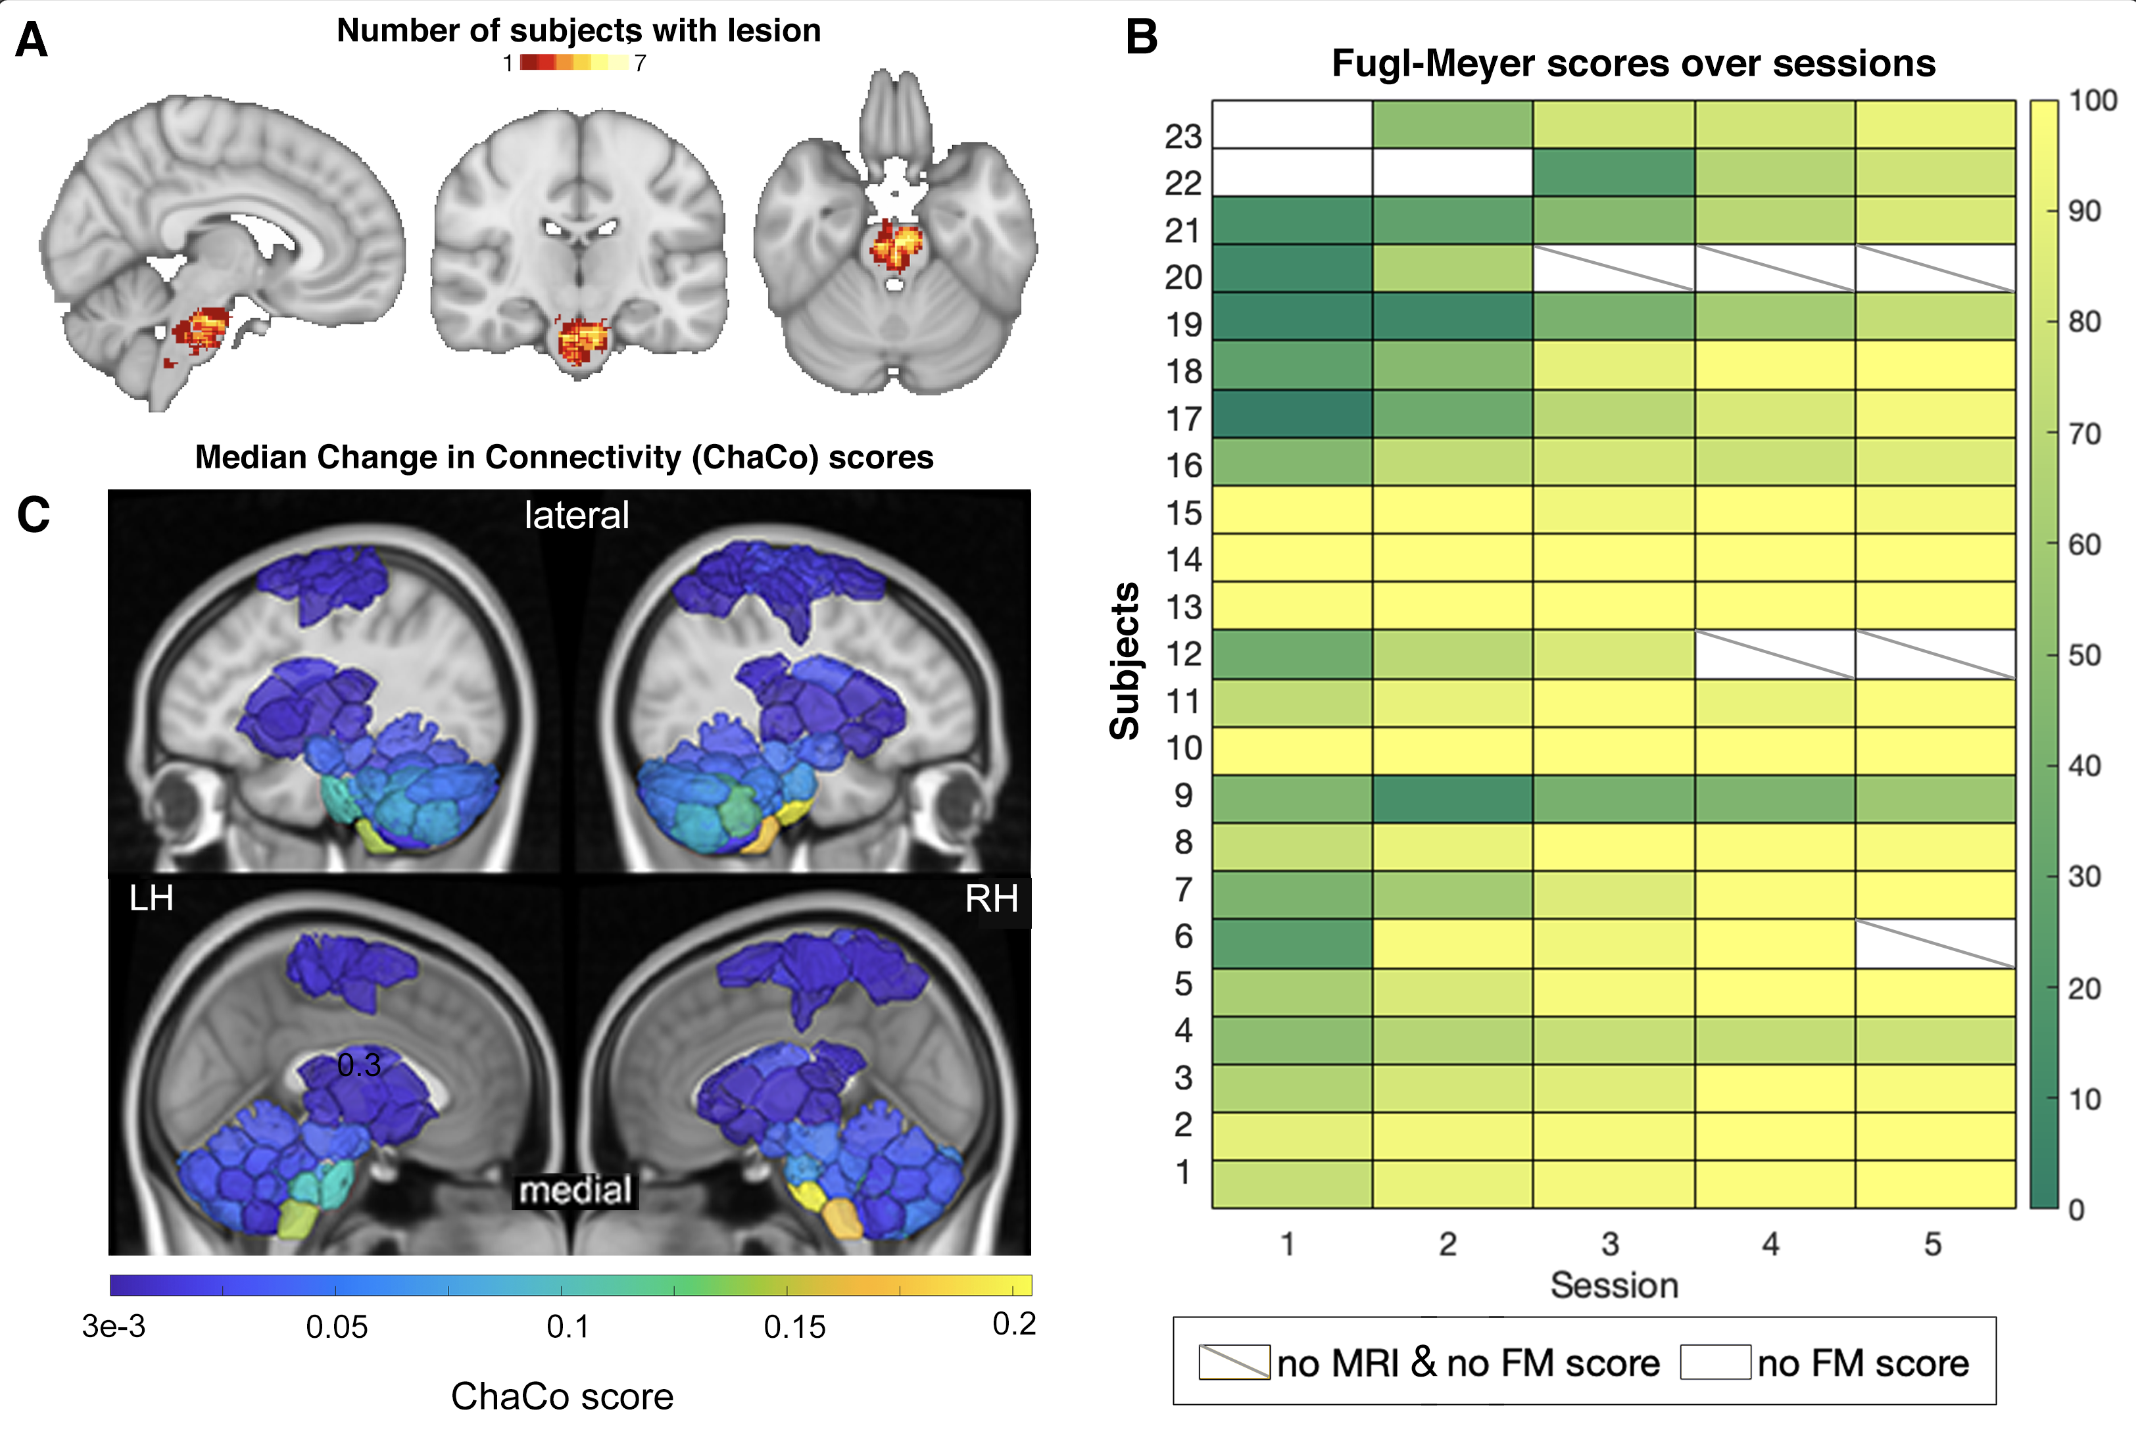
\includegraphics[width=\textwidth]{chapter1/Figure1.png}
       \caption{Overview of individuals' stroke lesions, resulting structural disconnection and Fugl-Meyer score trajectories. }
  \caption*{\textbf{A.} Distribution of lesions across the brain. Colors indicate the number of subjects with a lesion in that voxel. \textbf{B.} Normalized Fugl-Meyer scores for all subjects over the five post-stroke sessions. Boxes colored white indicate missing motor scores and diagonal lines within the box indicate missing MRI data for the corresponding time point.  \textbf{C.} Group median structural disconnection scores for each brain region calculated as the number of streamlines connected to each region that intersect with the lesion, normalized by the total number of streamlines connecting to that region (only displaying regions with ChaCo scores $>$ 0.003 corresponding approximately to log(ChaCo)$<$-6). Cortical areas with non-zero median ChaCo scores reflect motor regions at the end of disrupted corticospinal tracts. Top row of each subject inset shows a lateral view of the brain, bottom row of each inset shows a medial view.}
      \label{Figure1_1}
\end{figure}
\null
\vfill





%\subfloat[fig 2]{\includegraphics[width = 3in]{something}}\\
%\subfloat[fig 3]{\includegraphics[width = 3in]{something}}
%\subfloat[fig 4]{\includegraphics[width = 3in]{something}} 
%\caption{Add your own figures before compiling}


	\subsection{Structural data processing}
	Preprocessing of the longitudinal structural data included affine registration of each subject’s T1 scans to the baseline T1 scan, collapsing co-registered files to an average T1 and creation of a skull-stripped brain mask followed by manual editing and binarization of the hand-edited mask. The brain mask was then transformed back to each of the follow-up T1s in native space using the inverse registration acquired from the first step. This was followed by bias field correction of all the T1 scans, transformation of native-space bias field-corrected data back to baseline space, and the creation of an average bias field-corrected scan for each subject. Stroke lesion masks were hand-drawn on these transformed T1 scans by ADB and JEB. Structural normalization was performed with the CONN toolbox (\cite{Whitfield-Gabrieli2012-ox}). 
	
	\subsection{Functional data processing}
	Preprocessing of the longitudinal functional data was performed using the CONN toolbox (\cite{Whitfield-Gabrieli2012-ox}), including functional realignment of volumes to the baseline volume, slice timing correction for alternating acquisition, segmentation and normalization, and smoothing with a 4mm FWHM kernel. The WM and CSF probability maps used to derive WM and CSF BOLD signal were first thresholded above 50\% for each subject, and a one-voxel binary erosion step was applied to these thresholded maps (\cite{Whitfield-Gabrieli2012-ox}). This was followed by a denoising protocol (CompCor) (\cite{Behzadi2007-zt}) which regressed out the cerebrospinal fluid and white matter signal, as well as 24 realignment parameters (added first-order derivatives and quadratic effects). Temporal band pass filtering (0.008 - 0.09Hz), despiking and global signal removal regression were also performed. The first four frames of each BOLD run were removed. Frame censoring was applied to scans with a framewise displacement threshold of 0.5 mm along with its preceding scan (\cite{Power2012-tq}). Regional time series were acquired by parcellating the scans into 268 non-overlapping brain regions using a functional atlas derived from healthy controls (\cite{Shen2013-zn}) and averaging the time course of all voxels within a given region. Voxels identified as lesioned were excluded from regional timeseries calculations. Regions were assigned to one of 8 functional networks (Figure \ref{SupplementaryFigure1}), identified by (\cite{Finn2015-er}) using spectral clustering in healthy subjects.
	
	\subsection{Functional connectivity calculation}
	 Functional connectivity (FC) matrices were calculated as the regularized inverse of correlation matrices. Calculating FC using precision minimizes the effect of indirect connections and has been shown to result in connectomes that are more similar to structural connectivity (\cite{Wodeyar2020-kz, Liegeois2020-ua}). To compute the precision FC, we first calculated the full Pearson correlation-based FC ( \begin{Large}$\Sigma_i$ \end{Large}) for each individual $i$ by correlating region-pair time series. We then took the unregularized inverse of \begin{Large}$\Sigma_i$\end{Large}, denoted \begin{Large}$P_i$\end{Large}, and averaged them over the $i$ subjects to obtain the population-level precision FC matrix  \begin{Large}$P_{avg}$\end{Large}. We then calculated the individual precision FC matrices using Tikhonov regularization, which adds a full-rank regularization term (scaled identity) to the correlation matrix before inversion (\cite{Liegeois2020-ua}).
	 
\begin{Large}
\begin{center}

       $ P_i^{reg} = (\Sigma_i + \lambda \cdot I)^{-1}$

\end{center}
\end{Large}


    where $I$ is the identity matrix and $\lambda \in [0,1]$ is the regularization parameter. The regularization parameter $\lambda$ was chosen via a grid search to be the value that minimized the root mean squared error of the Frobenius norm of the difference in regularized subject precision matrices \begin{Large}$P_i^{reg}$\end{Large} and the population-level unregularized precision matrix \begin{Large}$P_{avg}$,\end{Large} which was found to be $\lambda = 0.71$ (Figure \ref{SupplementaryFigure2}). Partial correlation (precision) involves the inversion of the correlation matrix, and to stably invert this matrix, regularization is needed. Tikhonov regularization (a.k.a. L2 ridge regression), employed here, involves addition of an identity term scaled by a constant $\lambda$. The group average unregularized precision matrix is only used for the optimization of this $\lambda$ term, not in the matrix inversion, and is performed as previously described (\cite{Liegeois2020-ua, Golub1999-ou}). The unregularized group average precision matrix is used as a benchmark for tuning this hyperparameter, as some of the inversion noise has been smoothed out in the calculation of the average. The values along the diagonal were set to 0 prior to graph matching; this is a form of regularization that penalizes off-diagonal swaps, which we employ to control the effect of regions with low SNR; a noisy region will be more likely to be assigned to itself because the zeroes are aligned. For completeness, the main analyses have been replicated with Pearson correlation-based FC, and results are provided in the supplementary material (Figure \ref{SupplementaryFigure13}, \ref{SupplementaryFigure14}, \ref{SupplementaryFigure15}), with few differences to the overall findings with the precision FC.
    
	\subsection{Estimated structural disconnection}
	Deficits from subcortical stroke may be related to functional alterations at distant sites via metabolic diaschisis (\cite{Hillis2002-dz, Corbetta2015-ez}) or remote degeneration that spreads along the white matter connectivity network (\cite{Duering2015-iv, Cheng2015-jq}). In order to account for the impact of lesions on the structural connectome, the extent of regional structural connectivity (SC) disruption due to the lesion was assessed for each stroke subject with the Network Modification (NeMo) Tool (\cite{Kuceyeski2013-nk}). The NeMo Tool v2 requires only an individual’s lesion mask in MNI space, which was obtained as described above, to produce an estimate of structural disconnection to each brain voxel, or to each region in a user-defined atlas. The newest version of the NeMo Tool, originally published in 2013, includes a reference database of SC from 420 unrelated individuals from the Human Connectome Project’s (HCP) 1200 release (50 percent female, aged 25-35). The NeMo Tool begins by mapping the lesion mask into this healthy database’s collection of tractography streamlines that quantify likely white matter pathways. It then identifies streamlines that pass through the lesion mask and records the gray matter voxels/regions that are at the ends of that streamline. The NeMo Tool produces the regional structural disconnection vector (ChaCo score, Change in Connectivity) that is an estimate of the percent of damaged streamlines at each voxel or region in the atlas. ChaCo scores were calculated for each stroke subject and the median was taken across the sample to create a group-level structural disconnection map (Figure \ref{Figure1}C).

\clearpage
\null
\vfill
\begin{figure}[!hp]
\caption{Overview of the graph matching procedure.}
\caption*{\textbf{A.} Example of a pair of regions that remap. Region $i$ at 1 week post-stroke and  region $j$ at 2 weeks post-stroke have highly similar FC with the rest of the brain (moreso than region $i$ at 1 week to region $i$ at 2 weeks). The cost to remap $i$ to $j$ is low, and these regions would likely be remapped in the graph matching algorithm. \textbf{B.} The cost of remapping each region pair is used as input to the graph matching algorithm; the output of graph matching is the assignment of each region in one imaging session to a single corresponding region in the subsequent imaging session. If this assignment is to a different region, then it said to have "remapped". \textbf{C.} Three examples of permutation matrices of three subjects with varying amounts of remapping; black entries represent the assignment of a source node (y-axis) to its target node (x-axis).}
    \label{Figure1_2}
\end{figure}
\null
\vfill
\clearpage
\begin{figure}[h!]
		\ContinuedFloat
		\captionsetup{labelformat=adja-page}
    \centering
    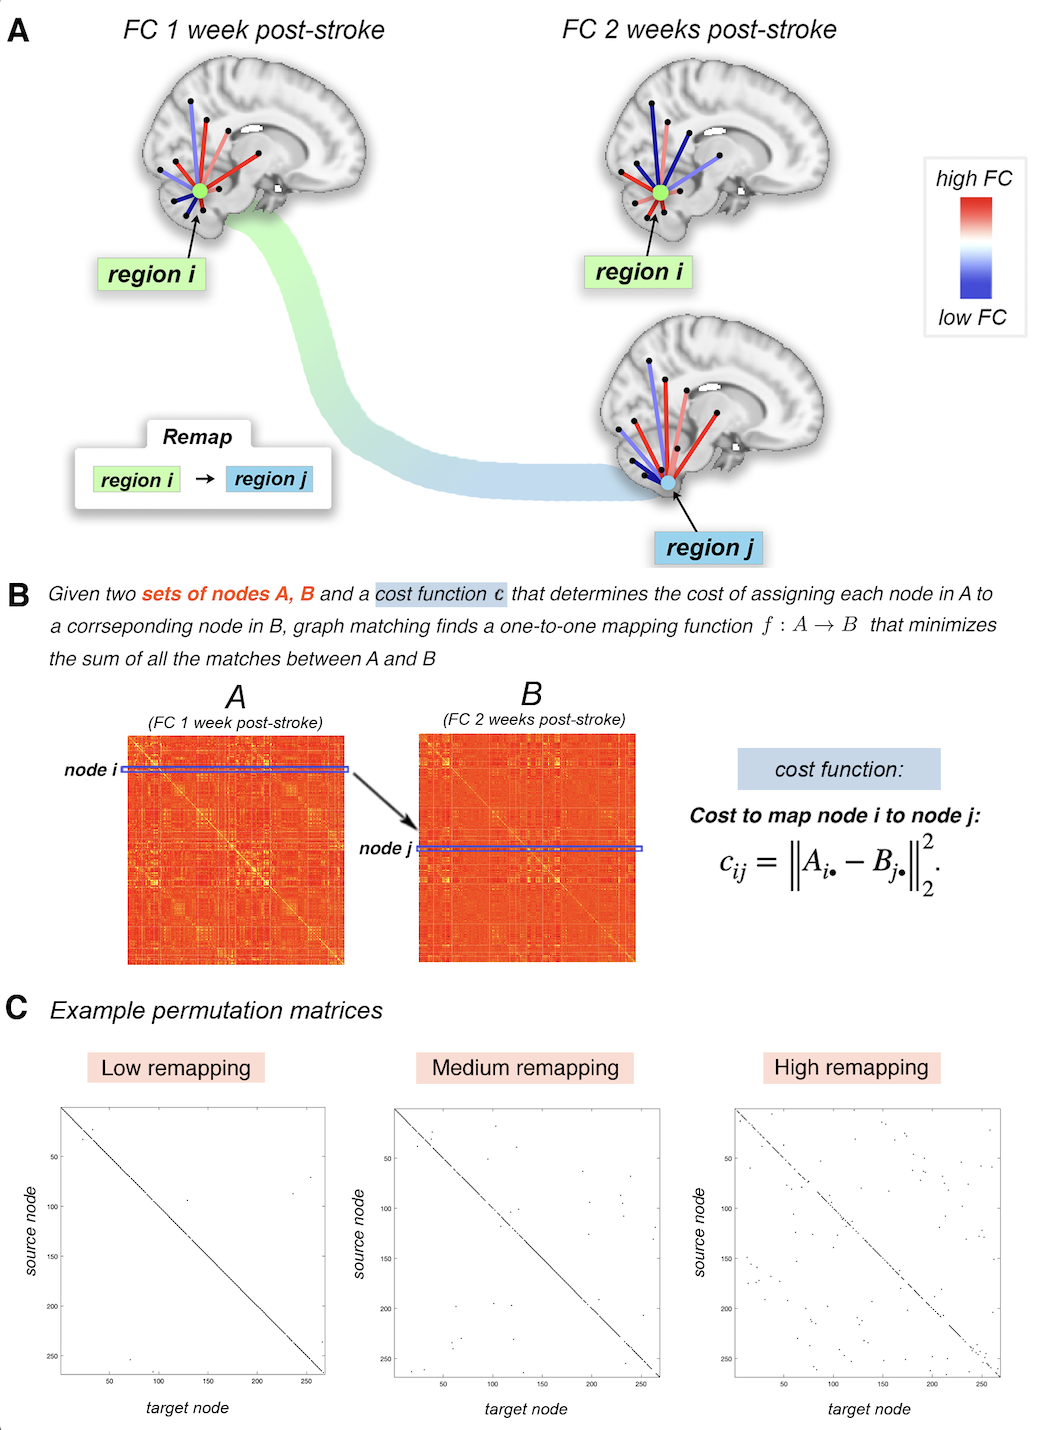
\includegraphics[width=\textwidth]{chapter1/Figure2.png}
    \caption[]{}
\end{figure}


	\subsection{Estimated functional disconnection}
	For each subject, we use FC matrices derived as described above to calculate the node strength, which quantifies the overall strength of all connections to and from a node, calculated the sum of all FC connection to the node (excluding a node's connection weight to itself). Then, for each time point, we performed an unpaired two-sided t-test at each node to determine whether its node strength was significantly different between stroke subjects and controls. The 268 p-values were corrected for multiple comparisons using Benjamini-Hochberg FDR correction at a corrected alpha of 0.05. We observed node strength disruptions in the stroke subjects at 1 week, 2 weeks, and 6 months post stroke, where stroke subjects had lower node strength in the brainstem, cerebellum, and temporal lobes compared to controls, and increased node strength in the lateral and medial frontal cortex (Figure \ref{SupplementaryFigure3}).
	
	\subsection{Graph matching}
	We used a graph matching algorithm to capture FC network reorganization over time (Figure \ref{Figure1_2}). Graph matching is an algorithmic process that maximizes the similarity between two networks by identifying an optimal mapping between nodes in the networks. One approach to identifying this optimal mapping is with a combinatorial optimization problem known as linear assignment. 
	
	Take two $n \times n $ networks $A$ and $B$ and a cost function $c: A \times B \rightarrow  \mathbb{R}$  that determines the cost of assigning each node in $A$ to each node in $B$. Entries in the cost matrix 
	\begin{Large}
	$C = (c_{i j})$
	\end{Large}
	 are defined by the Euclidean distance between row $i$ in $A$ and row $j$ in $B$, i.e. \begin{Large}$c_{ij}(A,B)=|| A_{i\bullet}-B_{j \bullet} ||^2_2$\end{Large}. In our application, the rows \begin{Large}$A_{i\bullet}$\end{Large} and \begin{Large}$B_{j \bullet}$\end{Large} represent region $i$ and region $j$'s FC to the rest of the brain, or FC profile, respectively. The linear assignment problem aims to construct the permutation matrix \begin{Large}$P = \big(p_{i j}\big)$\end{Large} that minimizes the sum of the elements in cost matrix, i.e. \begin{Large}$min_P\sum^n_{i=1}\sum^n_{j=1}c_{ij}p_{ij}$\end{Large} . The matrix $P$ is a permutation matrix with exactly one entry equal to 1 in each row and column, the rest being zero. Ones in the diagonal of $P$ indicate the same node in the two networks were mapped to one another, while ones in the off-diagonal indicate a node was “remapped” to another node.
	
	Here, we use the Hungarian algorithm to solve this minimization problem and find the corresponding optimal permutation matrix $P$. Figure \ref{Figure1_2} illustrates how the graph matching is applied to subsequent longitudinal FC networks in the same individual (either post-stroke or control) and depicts an instance of remapping in a single subject.  In Figure \ref{Figure1_2}A, the FC profile of brain region i (green region) at 1 week post-stroke is more closely matched by the FC profile of region j (blue region) at 2 weeks post-stroke than it is to itself at 2 weeks post-stroke. Example permutation matrices for three stroke subjects (one with high amount of remapping, one with an average amount of remapping and one with a low amount of remapping) are also provided. 
	
	\subsection{Quantification of functional reorganization}
	
	We make assumption that remapping in the healthy controls is due to noise. Then, to remove this noise, we observed the set of nodes to which node $x$ got assigned in the healthy control population along with their frequency. If node $x$ was assigned to node $y$ in more than 5 control subjects (across all time point intervals, i.e., $> 5 \%$ of the time), we remove this entry from the permutation matrices of all stroke subjects. All remaining entries after this removal procedure are considered as significant remappings. The rationale for this thresholding approach is that there may be remapping that happens longitudinally in controls that is either due to noise in the fMRI data or some other physiological noise that is unrelated to stroke recovery. Removal of these normative effects will allow better isolation of remapping likely to be related to the post-stroke reorganization process. Because using the cutoff of 5 control subjects is an arbitrary choice, we have replicated the main analyses using a cutoff of 1 (i.e., remove remap of node $x$ to node $y$ from stroke subjects if node $x$ was assigned to node $y$ in 1 or more control subjects (across all time point intervals, i.e., $> 1 \%$ of the time). The results with this more conservative threshold are provided in the supplementary materials, and are very similar to the main results (Figure \ref{SupplementaryFigure16}, \ref{SupplementaryFigure17}, \ref{SupplementaryFigure18}).

	The permutation matrices, calculated for each pair of time points, were then used to quantify functional reorganization. We defined functional remapping at three levels:
	
	\begin{itemize}
	 \item \textbf{Subject level}: To assess the amount of functional reorganization in an individual, the number nodes that were remapped (sum of the off-diagonal in $P$) between each time point interval was calculated. This referred to as the 'number of remaps' between subsequent imaging sessions for a single subject.
	 
	 \item \textbf{Node level}: To assess the spatial pattern of reorganization across the brain, we calculated each node's 'remap frequency', i.e. the proportion of individuals that had that brain region remap between two subsequent time points.
	 
	 \item \textbf{Network level}: To assess the network-level pattern of reorganization, we calculated the sum of remaps within and between 8 functional brain networks across all subjects. Since there are 8 networks, there are 64 possible source network/target network combinations (including the phenomenon of a node in a network remapping to a different node within the same network). We normalized each sum by the number of subjects, and then by the number of nodes in the source network. This value therefore expresses the proportion of remaps between networks, per subject, adjusted for the total number of possible remaps in each network. 
	\end{itemize}

	\subsection{Statistical analyses}
	To test the hypothesis that brain regions more structurally disconnected by the stroke lesion would have more frequent remapping, we calculated the correlation between the node remapping frequency and the sample median log-transformed ChaCo scores that quantify the regional amount of white matter connectivity disruption due to the stroke lesion. We removed nodes which had non-zero overlap with each subject's lesion in the calculation of the median ChaCo score to exclude the effect of direct damage from the lesion. To test the hypothesis that brain regions more functionally disconnected by the stroke lesion would have more frequent remapping, we calculated the correlation between the node remapping frequency and the t-statistic of the node strength. The statistical significance of the correlations described above were assessed with permutation testing. 
	
	There are four subject-level remapping values for each subject, representing 4 time point comparisons post-stroke: 1 week - 2 weeks, 2 weeks - 1 month, 1 month - 3 months and 3 months - 6 months. Because there was a statistically significant correlation between scan length and remapping for the time point from 1 week - 2 weeks post-stroke (Figure \ref{SupplementaryFigure4}), the fMRI scan lengths of both time points were included as covariates in analyses concerning remapping over time. 
	
	To test the hypothesis that individuals with more baseline remapping would have greater initial motor impairment, we calculated the Pearson correlation between Fugl-Meyer motor scores at 1 week post-stroke and subject-level remapping from 1 week to 2 weeks post-stroke. To test the hypothesis that individuals with more baseline remapping would have greater motor recovery at 6 months, we calculated the Pearson correlation between the change in Fugl-Meyer motor scores from 1 week to 6 months post-stroke and subject-level remapping from 1 week to 2 weeks post-stroke. 
	
	To test the hypothesis that individuals with more remapping from one time point to another have better motor improvement, we calculated the Pearson correlation between change in Fugl-Meyer motor scores and subject-level remapping from one time point to the next for all four pairs of subsequent time points.This analysis enables us to identify whether remapping within a particular time point interval is more or less associated with motor improvement. In order to leverage the repeated subject measurements, a linear mixed effects regression model was employed to determine the relationship between the amount of remapping between sessions and the change Fugl-Meyer score between sessions, including age, sex, and scan length as covariates.  Let $i$ index a subject, \begin{Large}$t_{ab}$\end{Large} index a time point interval (\begin{Large}$t_a$\end{Large} = first time point, \begin{Large}$t_b$\end{Large} = second time point, and  \begin{Large}$t_{ab}$\end{Large} = the time point interval). Our model is then (split across 2 lines): 
	
	\begin{Large}
	\begin{center}

	$changeFM_{it_{ab}} =  \beta_0 + \beta_1 remapping_{it_{ab}} + $
	$ \beta_2 scan length_{it_a} +\beta_3 scan length_{it_b} + \beta_4 age_i + \beta_5 sex_i + b_i + \epsilon_{it_{ab}}$

	\end{center}
	\end{Large}
	\noindent where \begin{Large}$b_i \sim N(0, \sigma_1^2)$ \end{Large} and \begin{Large}$\epsilon_{it_{ab}} \sim N(0, \sigma_2^2)$.\end{Large}  We include the random effect \begin{Large}$b_i$\end{Large} to account for correlation within a subject at different time points. 

	\subsection{Code availability}
	 The code for to replicate this analysis is available on GitHub: https://github.com/emilyolafson/stroke-graph-matching
	
	
\section{Results}
	\subsection{Functional reorganization is primarily observed in the brainstem and cerebellum}
	At the node level, remapping occurred most often in the brainstem and cerebellum (Figure \ref{Figure1_3}A,B), similar to the spatial distribution of median ChaCo scores (amount of structural disconnection) across the stroke sample, which were also highest in the brainstem and cerebellum (Figure \ref{Figure1_2}C). We also calculated group-level structural connectivity disruption in an approach more analogous to node remapping, by binarizing ChaCo scores into 'disrupted' and 'nondisrupted' nodes and calculating frequency of disrupted nodes over the population, with similar results (Figure \ref{SupplementaryFigure5}). For this paper, regional ChaCo scores were chosen over disconnection frequencies in order to preserve information about the magnitude of the disconnection. We hypothesize that the magnitude of disconnection influences whether a region is remapped or not.
	
	Next, we assessed network-level remapping within 8 functional networks. The most remaps were observed in the subcortical-cerebellum network (Figure \ref{Figure1_3}C,D) and in particular between contralesional nodes in the subcortical/cerebellum network (Figure \ref{SupplementaryFigure6}).
	
\clearpage
\null
\vfill
\begin{figure}[!hp]
\caption{Visualization of node-level remapping frequencies and group-level structural connectivity disruptions due to the lesion.}
\caption*{ \textbf{A.} Node remap frequencies are plotted on a glass brain  averaged across 4 time point comparisons (only displaying values above 0.1, for clarity). Inset figures display a lateral view (top row) and medial view (bottom row). \textbf{B.} Node remap frequencies $>0.1$ plotted on a glass brain, displayed separately for each time point comparison. \textbf{C.} Network-level sum of remaps. Remaps are separated based on their position relative to the lesion (contralesional vs. ipsilesional). \textbf{D.} Network-level sum of remaps, displayed separately for each time point comparison. Ipsilesional = same hemisphere as the lesion, contralesional = opposite hemisphere as the lesion}
    \label{Figure1_3}
\end{figure}
\null
\vfill
\clearpage
\null
\vfill
\begin{figure}[h!]
		\ContinuedFloat
		\captionsetup{labelformat=adja-page}
    \centering
    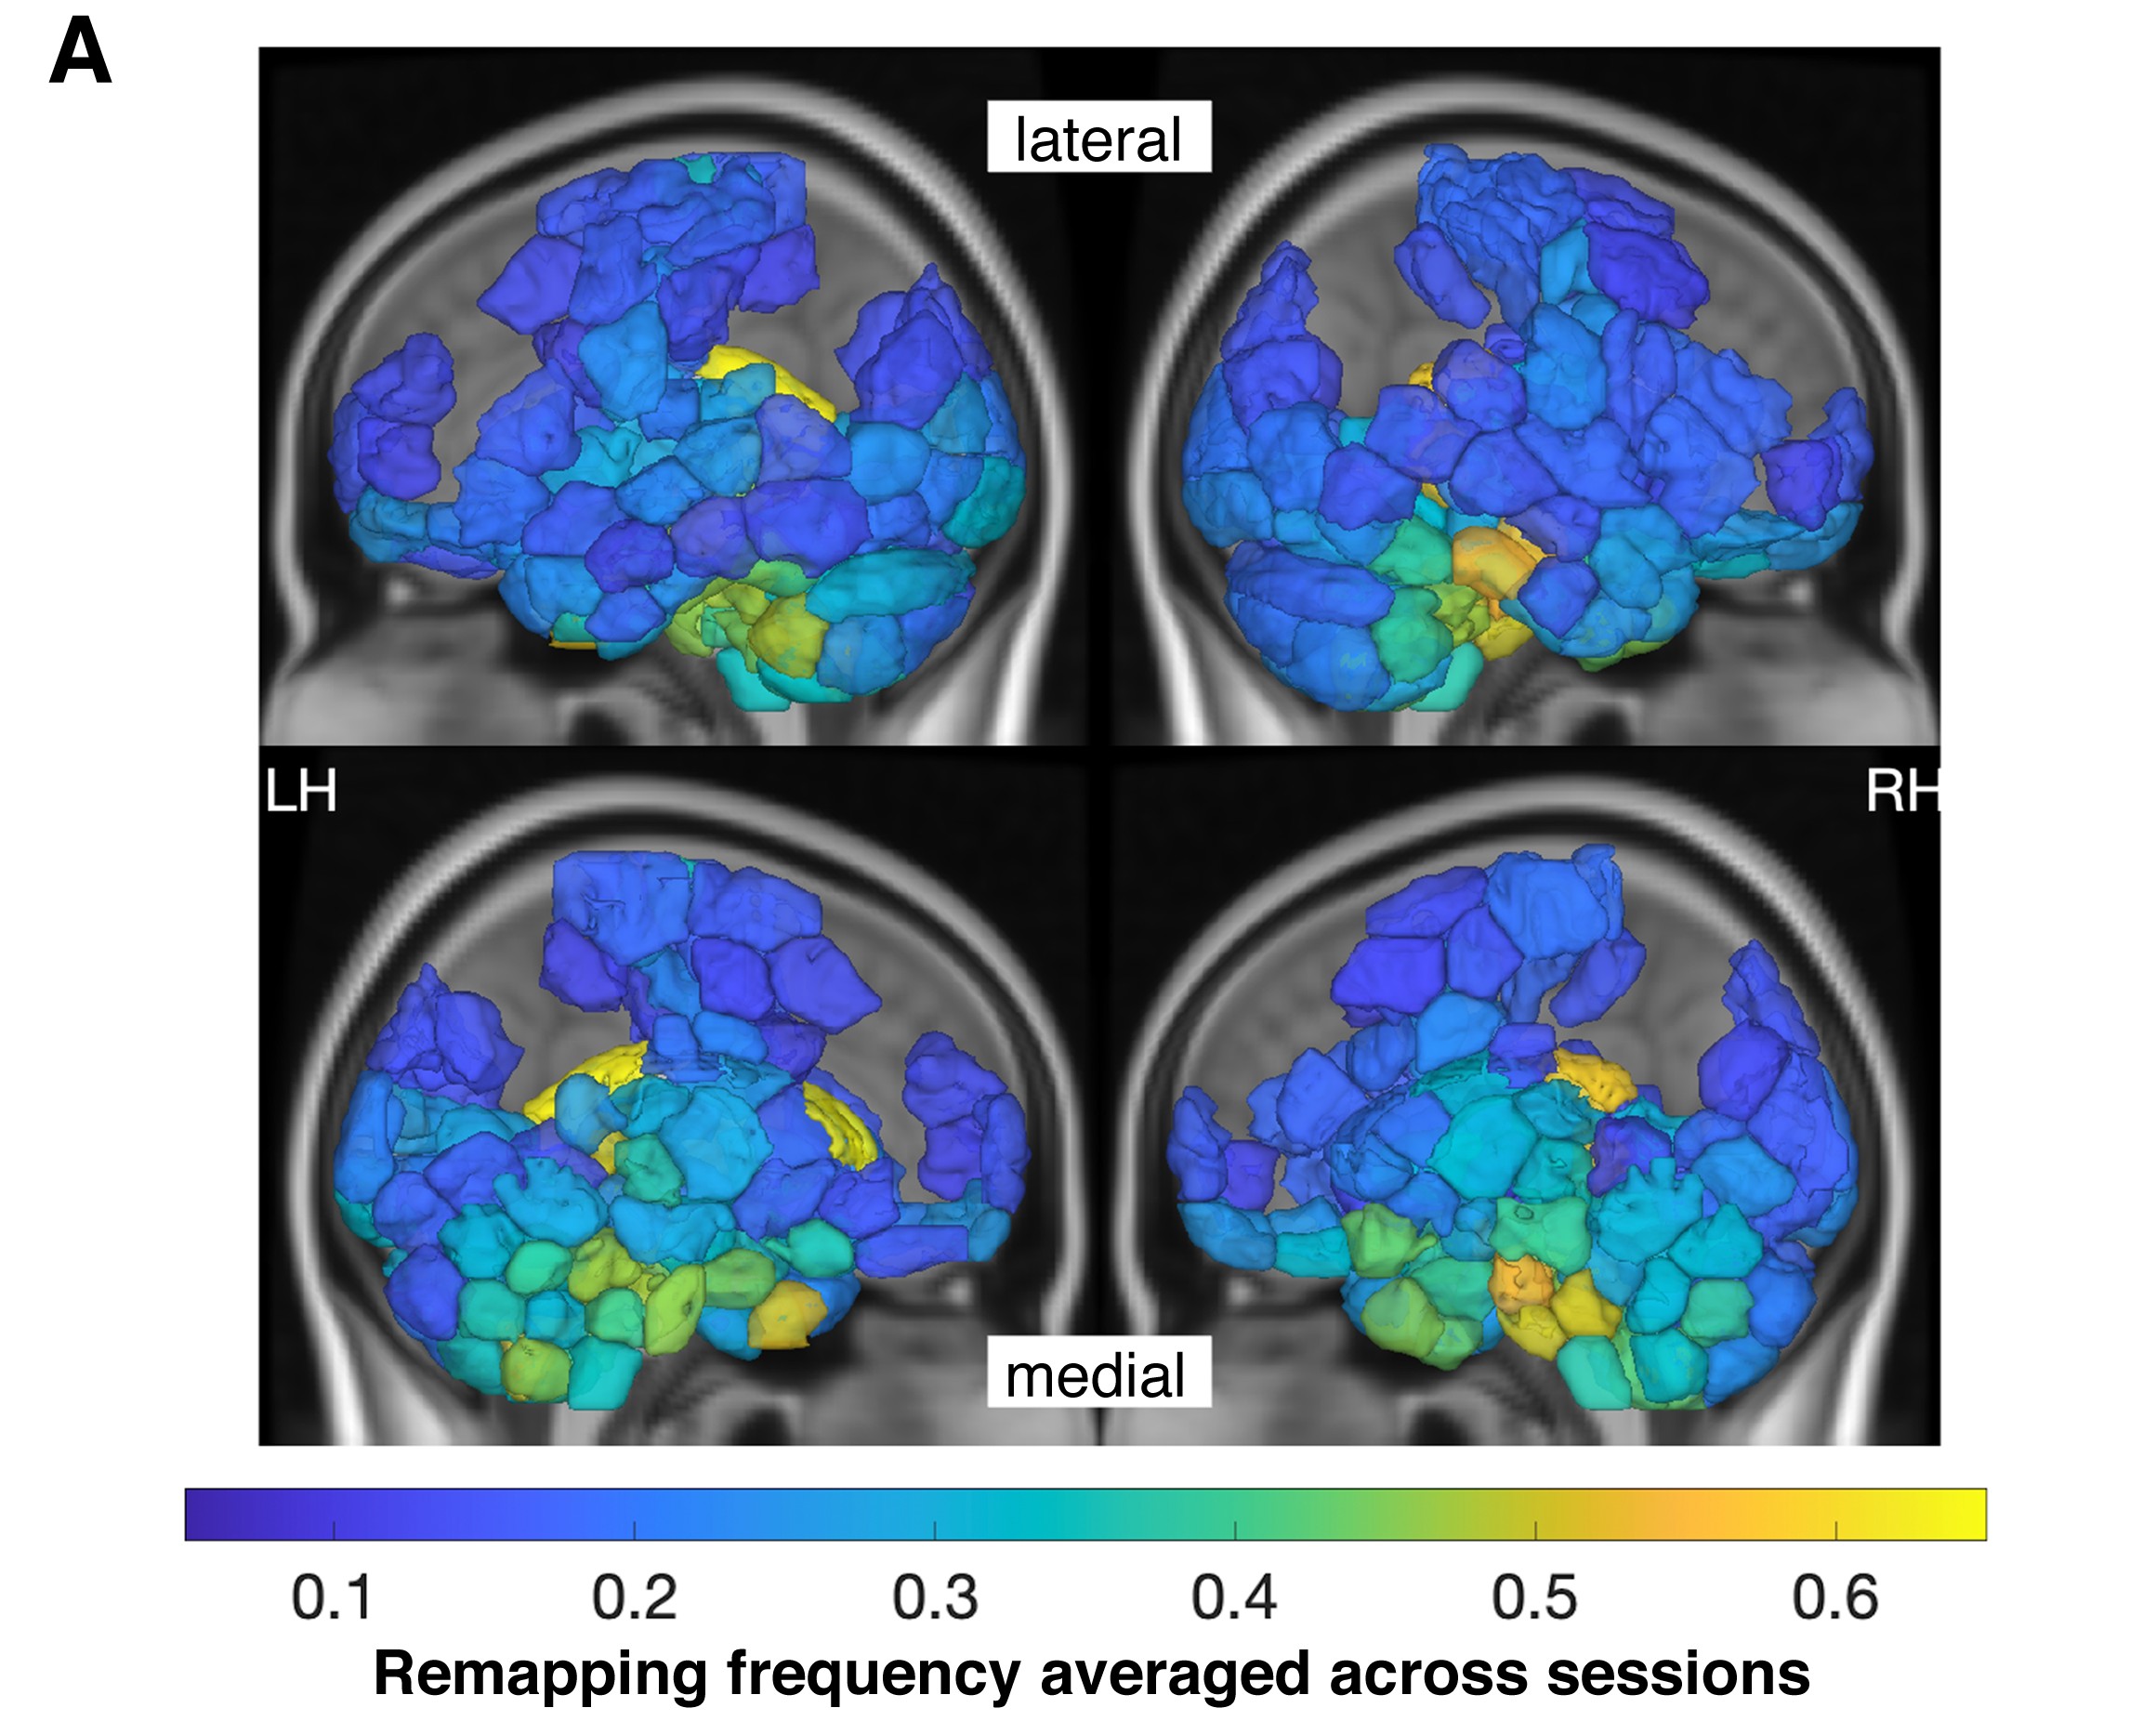
\includegraphics[width=\textwidth]{chapter1/Figure3A.png}
    \caption[]{}
\end{figure}
\null
\vfill
\clearpage
\null
\vfill
\begin{figure}[h!]
		\ContinuedFloat
		\captionsetup{labelformat=adja-page}
    \centering
    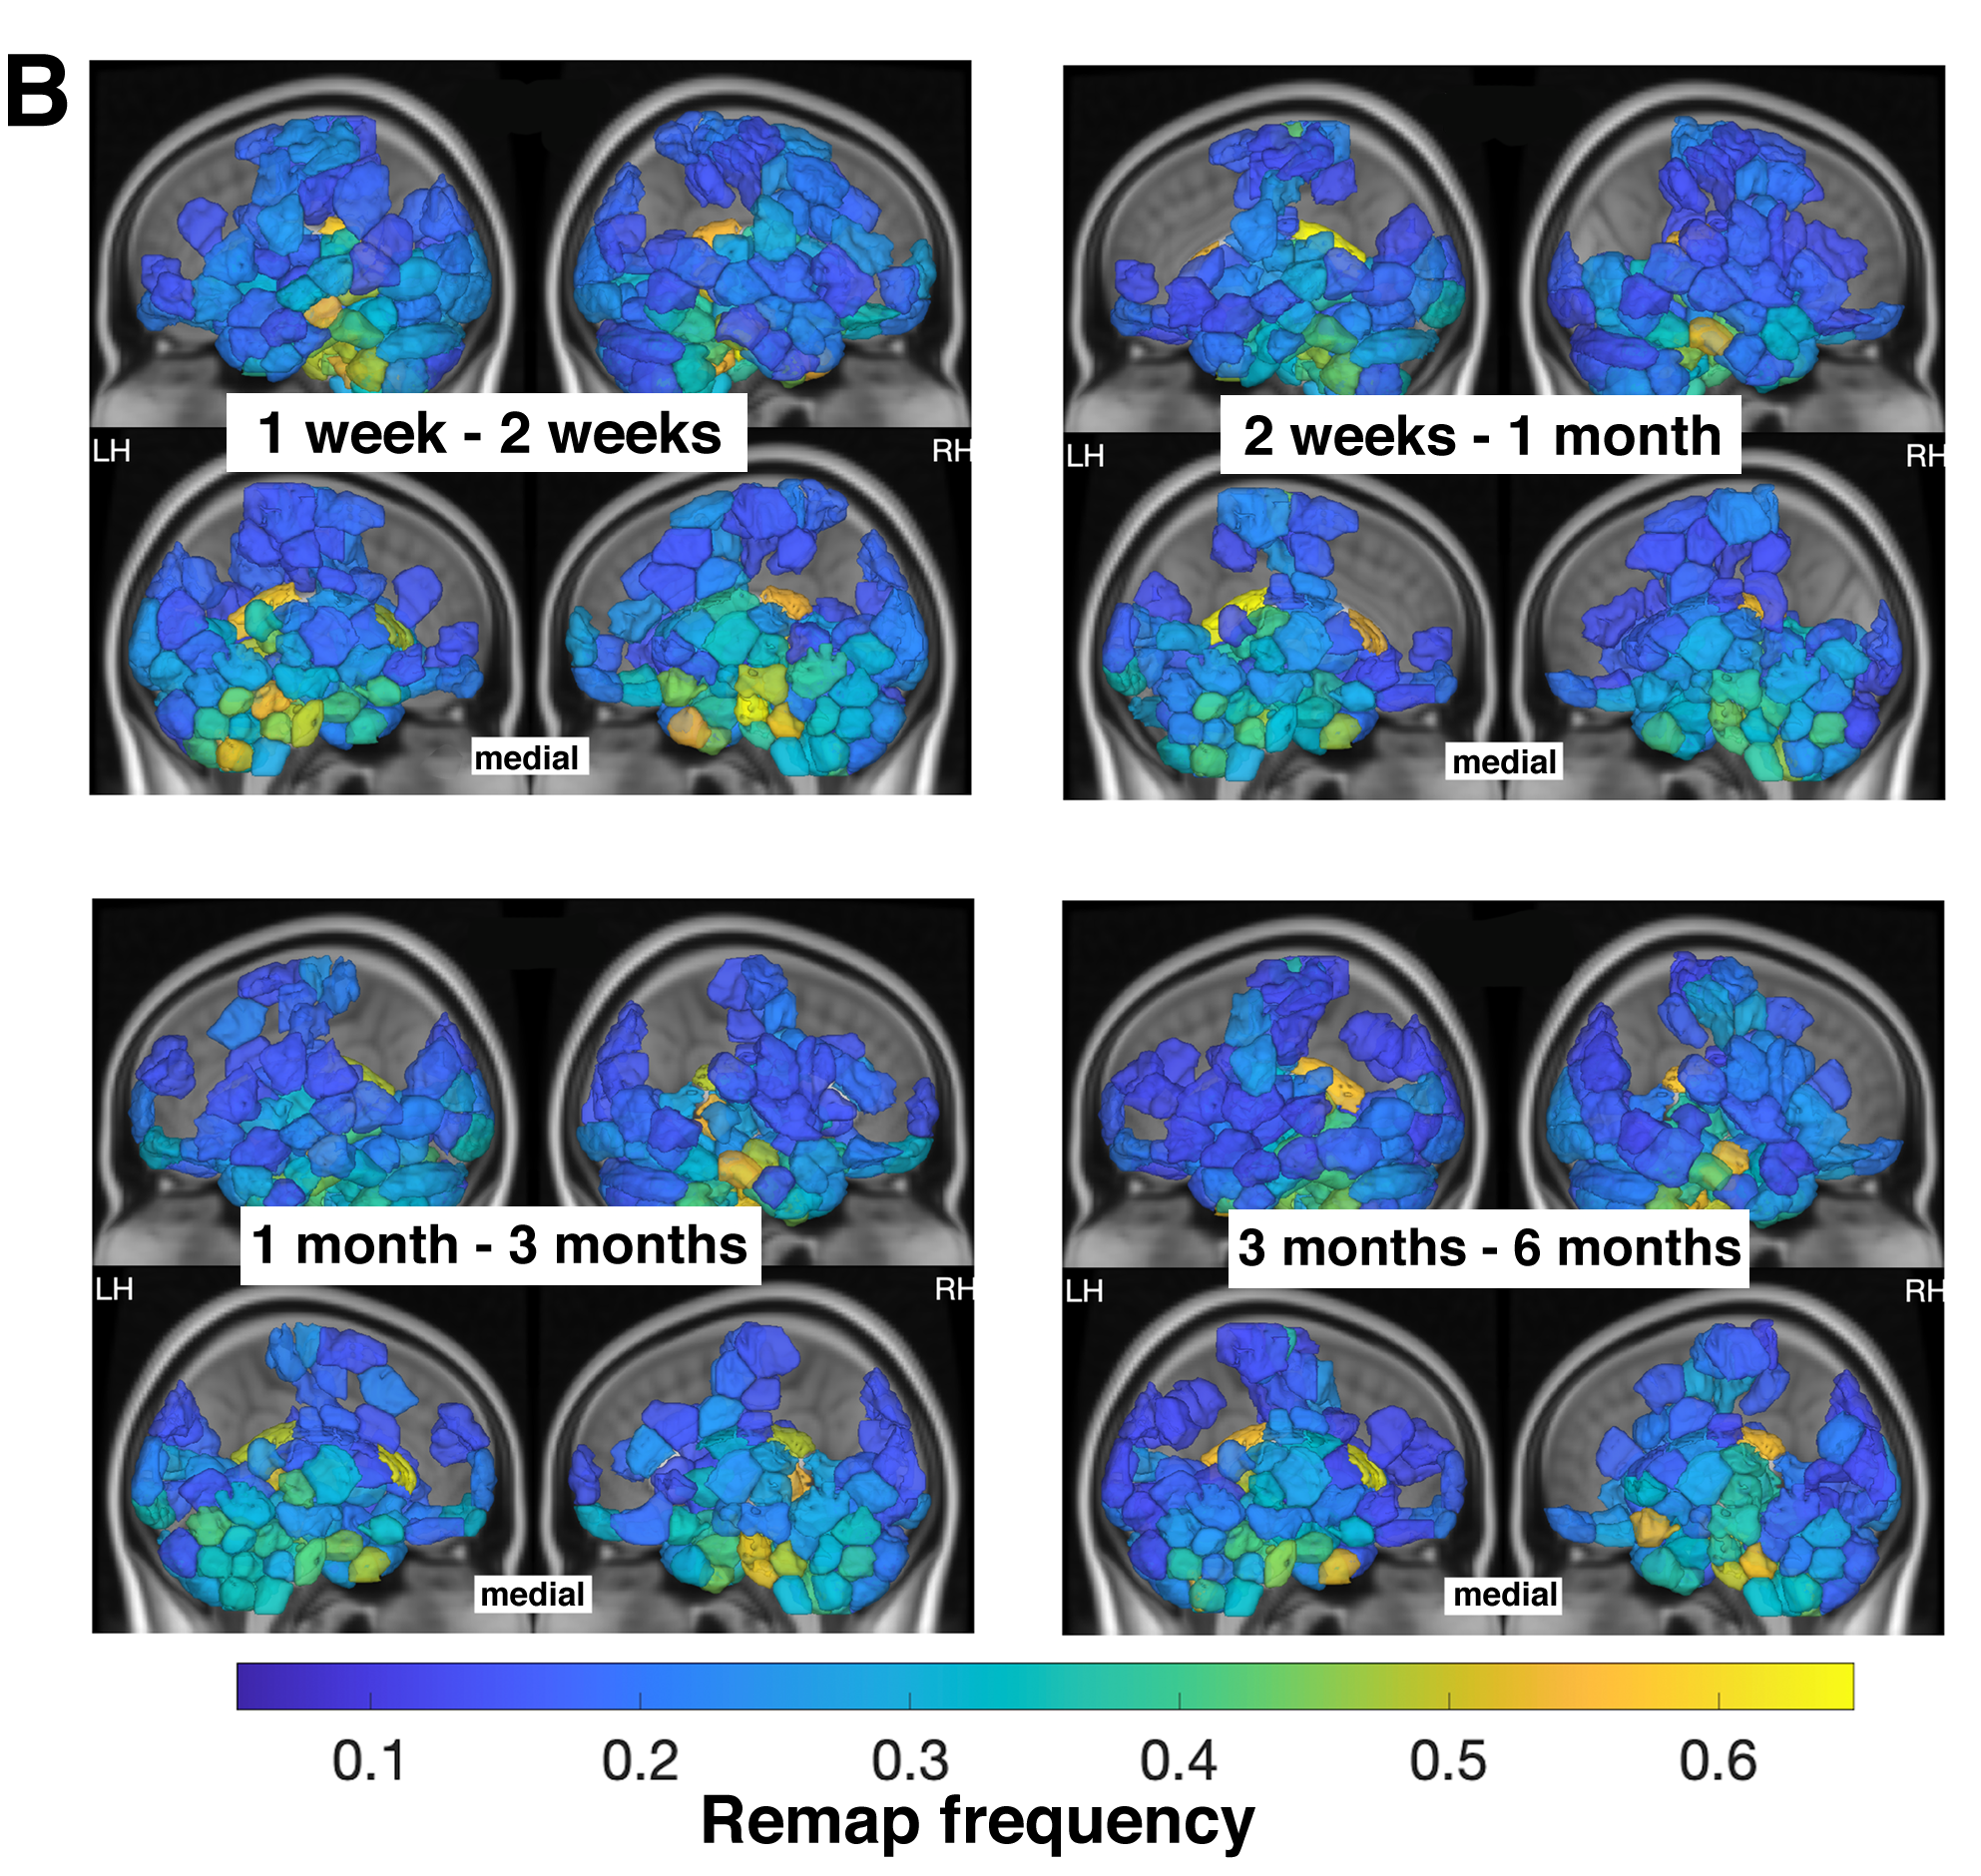
\includegraphics[width=\textwidth]{chapter1/Figure3B.png}
    \caption[]{}
\end{figure}
\null
\vfill
\clearpage
\null
\vfill
\begin{figure}[h!]
		\ContinuedFloat
		\captionsetup{labelformat=adja-page}
    \centering
    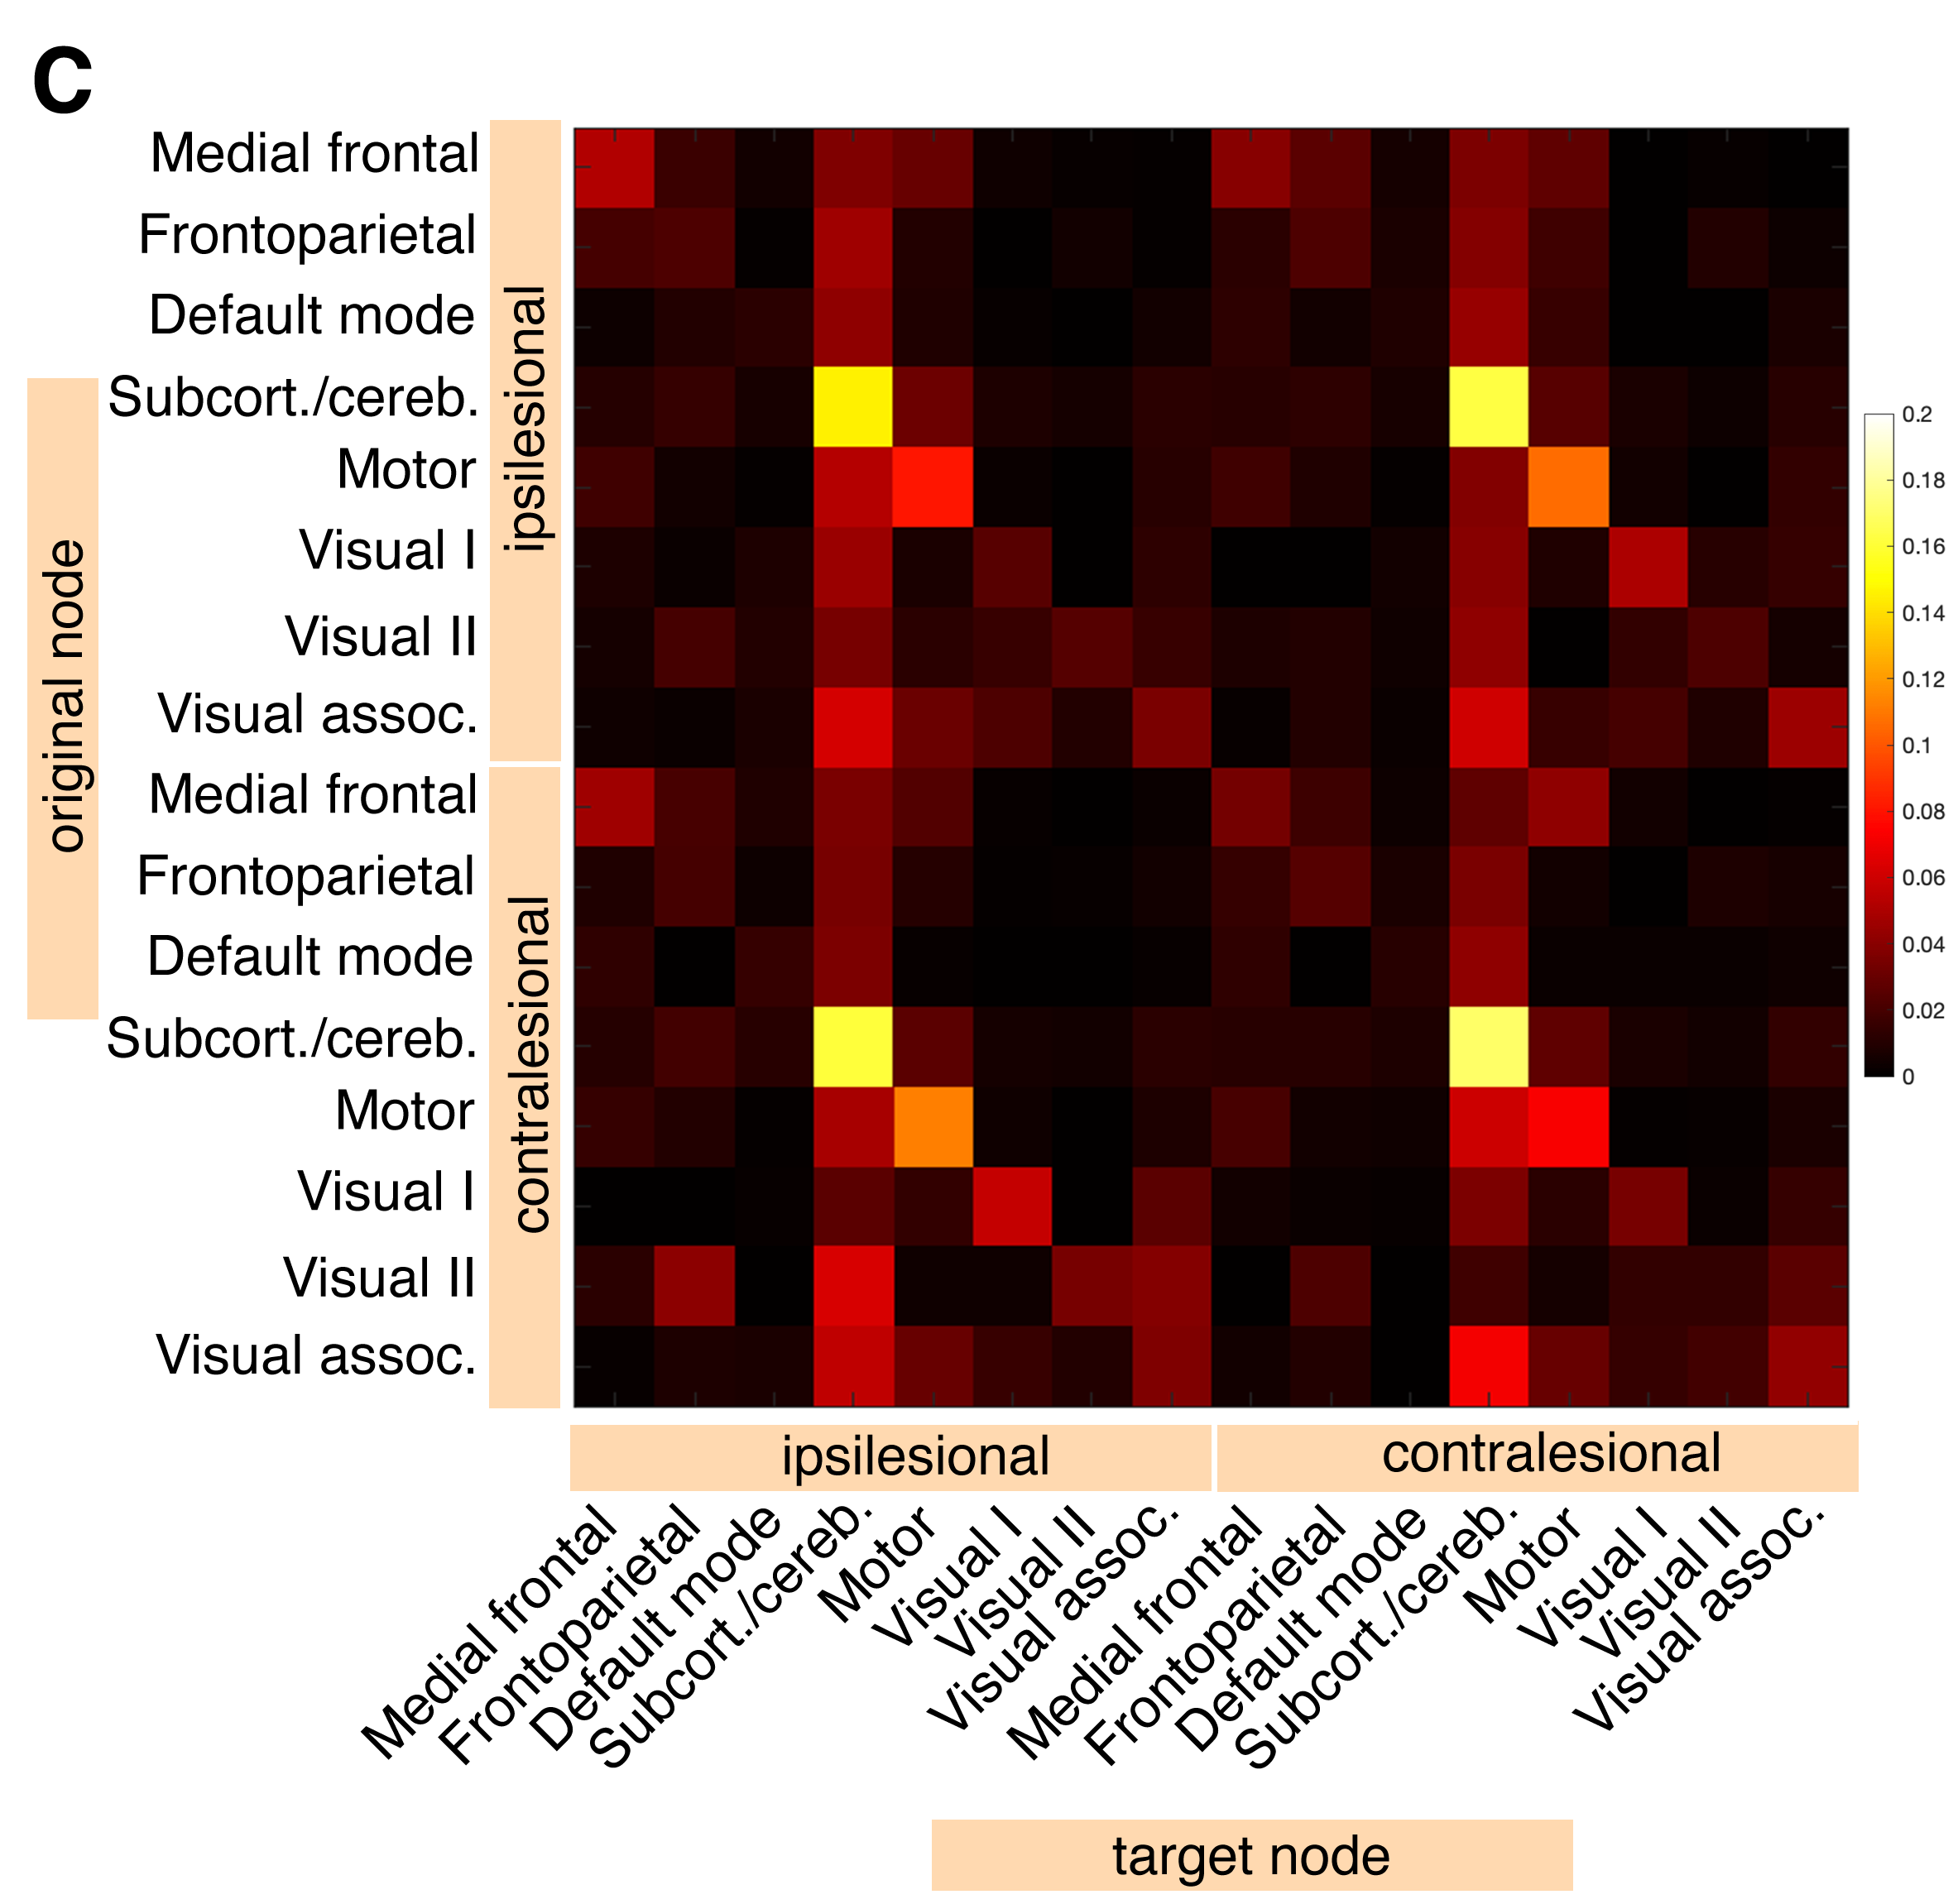
\includegraphics[width=\textwidth]{chapter1/Figure3C.png}
    \caption[]{}
\end{figure}
\null
\vfill
\clearpage
\null
\vfill
\begin{figure}[h!]
		\ContinuedFloat
		\captionsetup{labelformat=adja-page}
    \centering
    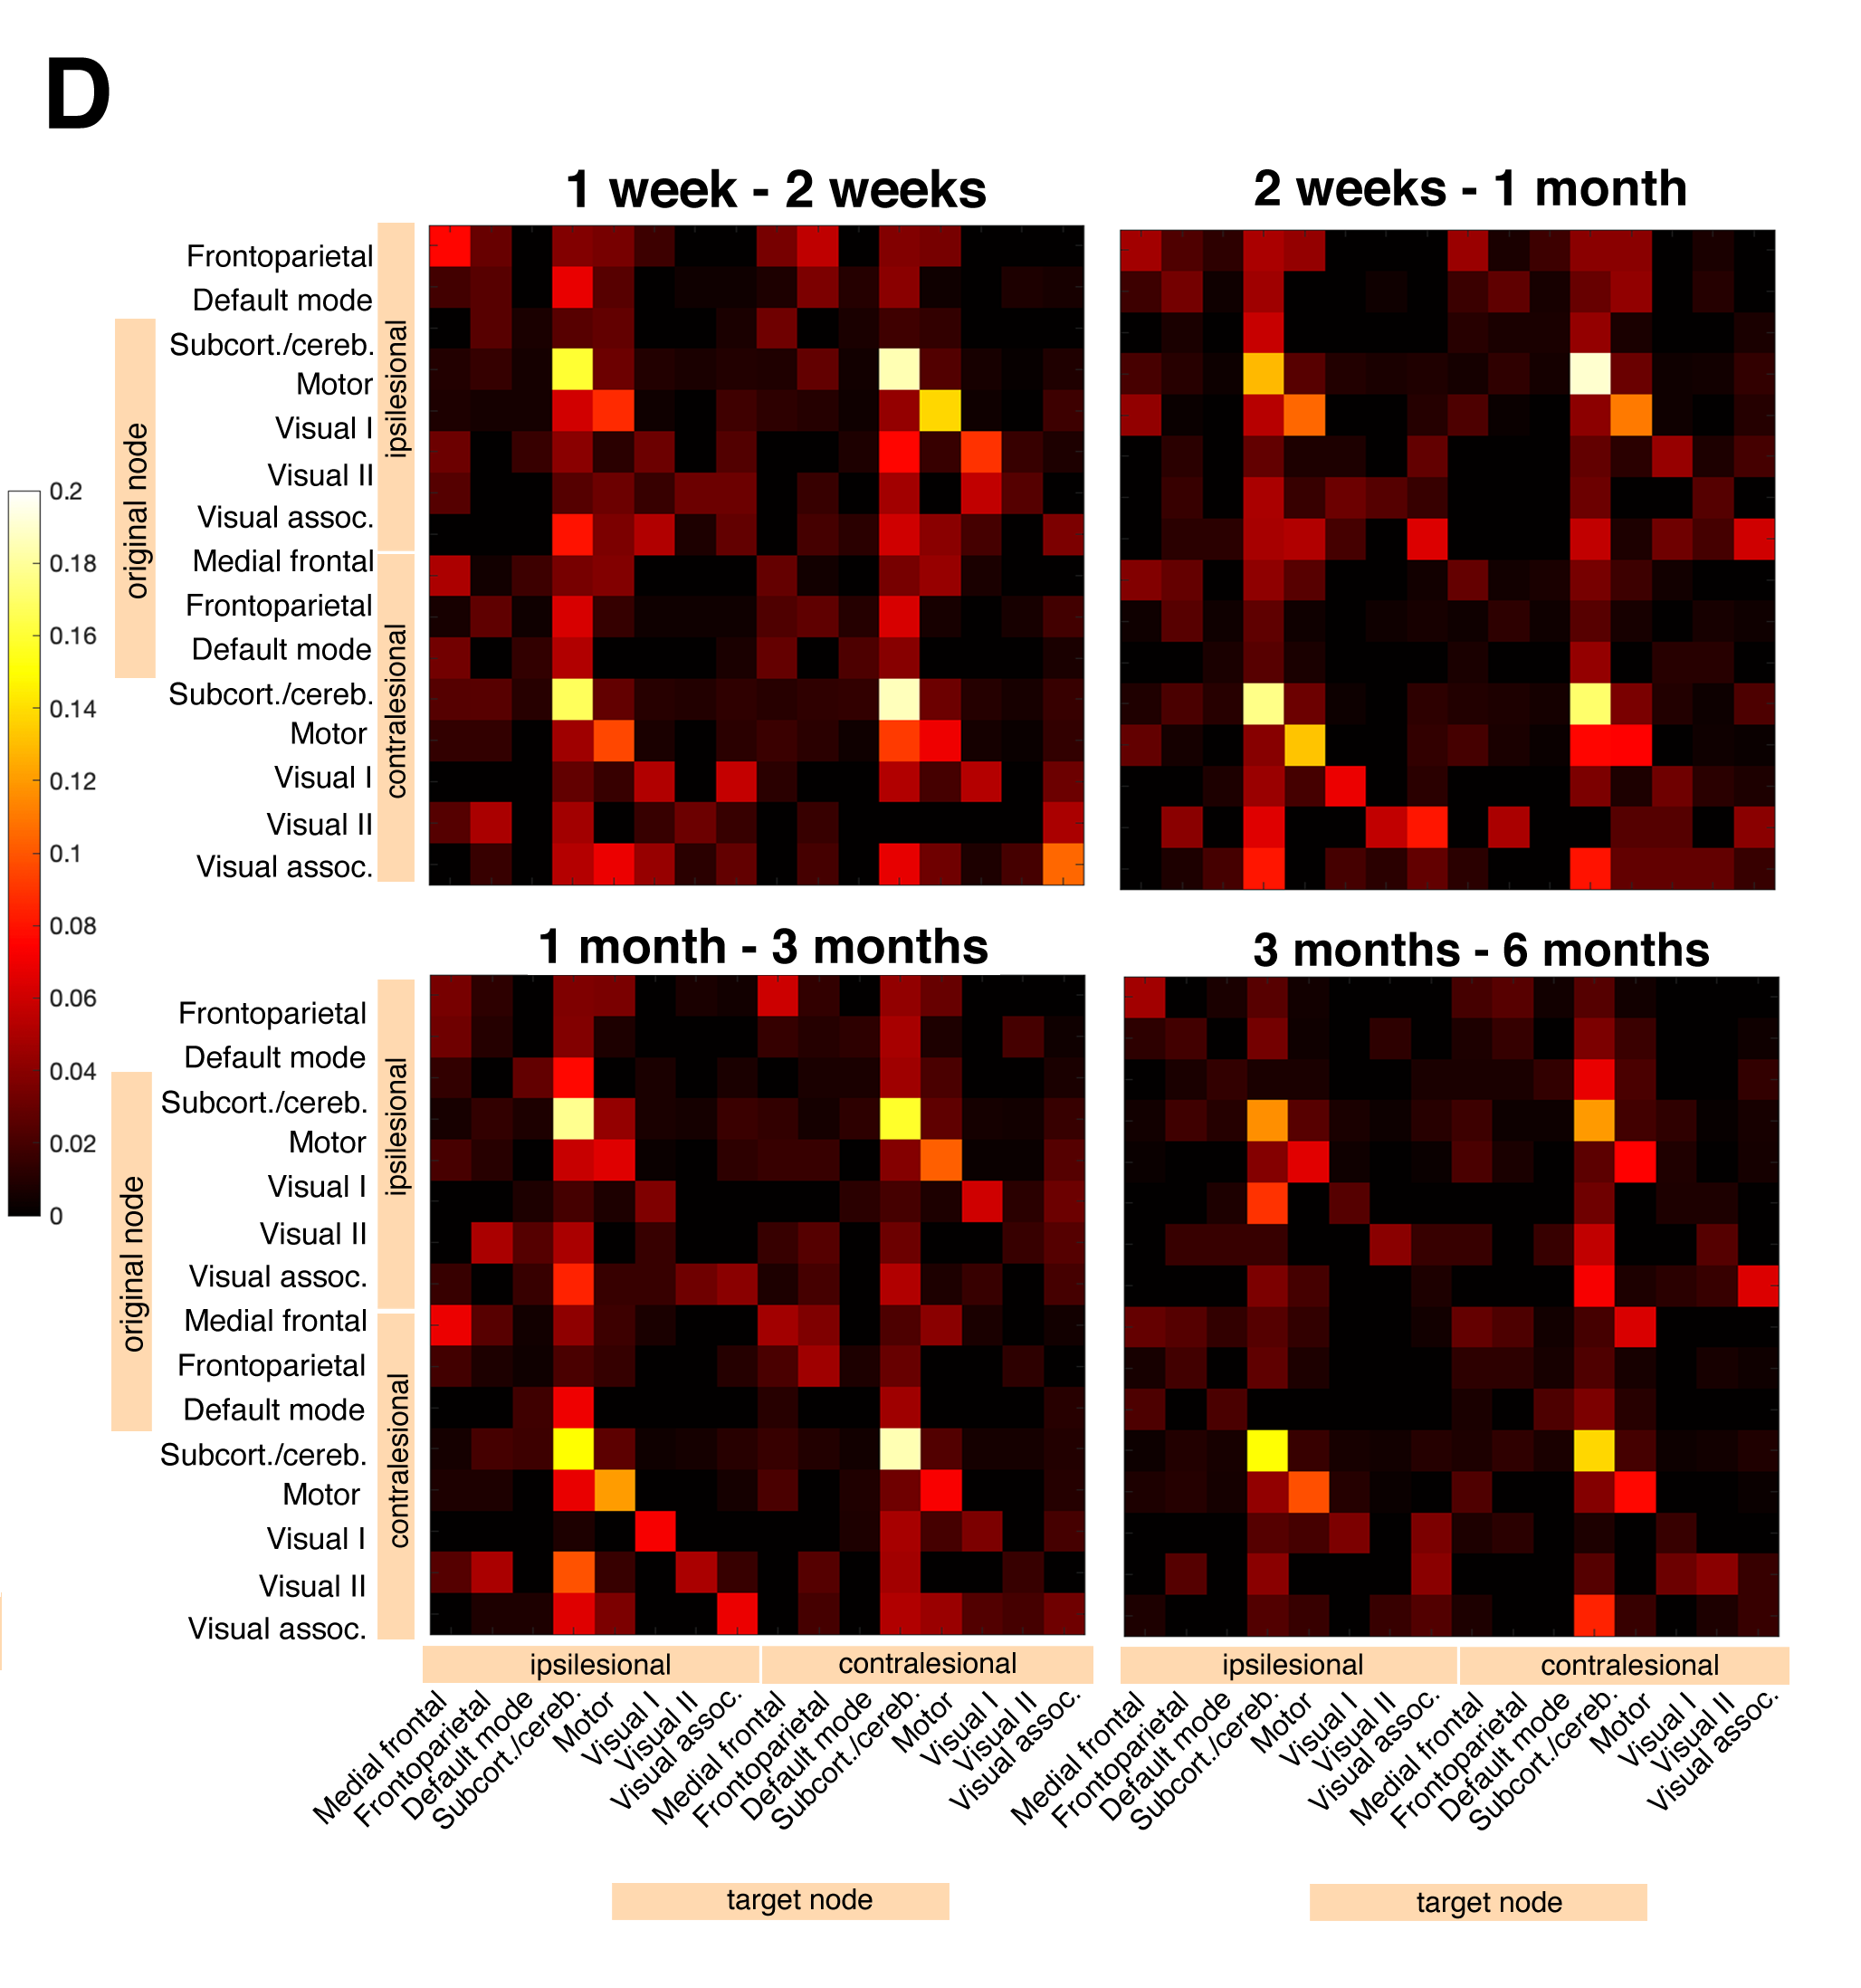
\includegraphics[width=\textwidth]{chapter1/Figure3D.png}
    \caption[]{}
\end{figure}
\null
\vfill
\clearpage

	\subsection{Regions with greater structural and functional disconnection  have more functional reorganization over time}
	There was a significant, positive correlation between node remapping frequency and median regional ChaCo scores from 1 to 2 weeks post-stroke ($r$ = 0.22, p = 3.05e-4), such that those regions with more structural connectivity disruption across the stroke subjects also had more remapping over time (Figure \ref{Figure1_4}A). This relationship was observed across all time points (Figure \ref{SupplementaryFigure7}A), and furthermore, across subjects, the brain regions that remap have significantly higher ChaCo scores compared to those that do not remap (assessed with permutation testing with 10000 permutations) (Figure \ref{SupplementaryFigure7}B).
	
	On the other hand, node remapping frequency at 1-2 weeks post stroke was negatively correlated with node strength relative to healthy controls at 1 week post-stroke ($r$  = -0.44, p = 2.62e-14) (Figure \ref{Figure1_4}B), where regions with lower node strength relative to controls at 1 week underwent the most remapping between 1-2 weeks post-stroke. This relationship was present across all time points (Figure \ref{SupplementaryFigure10}, \ref{SupplementaryFigure11}, \ref{SupplementaryFigure12}) and the correlation is very similar when using the first or second node strength measurement (Figure \ref{SupplementaryFigure9}).
	
	The nodes that underwent the most remapping were the most structurally and functionally disconnected, but the relationship between structural and functional disconnection is non-linear (Figure \ref{Figure1_4}C). Instead, the relationship between SC and FC disruption is impacted by the magnitude of the structural disruption. As seen in Figure S8, there is a clear cutoff for regions consistently structurally disrupted across subjects, corresponding to a ChaCo score of 0.003 (log(ChaCo) of -6). For regions exceeding a ChaCo score of 0.003 (i.e., with high structural connectivity disruption), there was a significant negative correlation between relative node strength and ChaCo scores ($r$  = -0.50, p = 2.1e-6)(Figure \ref{Figure1_4}D) and for regions below a ChaCo score of 0.003 (i.e., with little/no structural connectivity disruption), there was a significant positive correlation between relative node strength and ChaCo scores ($r$  = 0.49, p = 4.78e-13)(Figure \ref{Figure1_4}E). 



    

\clearpage
\null
\vfill
\begin{figure}[!hp]
\caption{Relationships between FC disruption, SC disruption, and remapping over the 1 week - 2 week time interval post-stroke. }
\caption*{\textbf{A.} Correlation between node remapping frequency and t-statistic of node strength. A jitter of 0.01 was added to data points along the x-axis to increase visibility. \textbf{B.} Correlation between node remapping frequency and ChaCo scores. A jitter of 0.01 was added to data points along the x-axis to increase visibility. \textbf{C.} Correlation between t-statistic of node strength and ChaCo scores. Dashed horizontal line at y = -6 represents the cut off point of log(ChaCo) -6, representing more SC disruption shown in \textbf{D}, below -6 representing minimal SC disruption is shown in \textbf{E}.}
    \label{Figure1_4}
\end{figure}
\null
\vfill
\clearpage
\null
\vfill
\begin{figure}[h!]
		\ContinuedFloat
		\captionsetup{labelformat=adja-page}
    \centering
    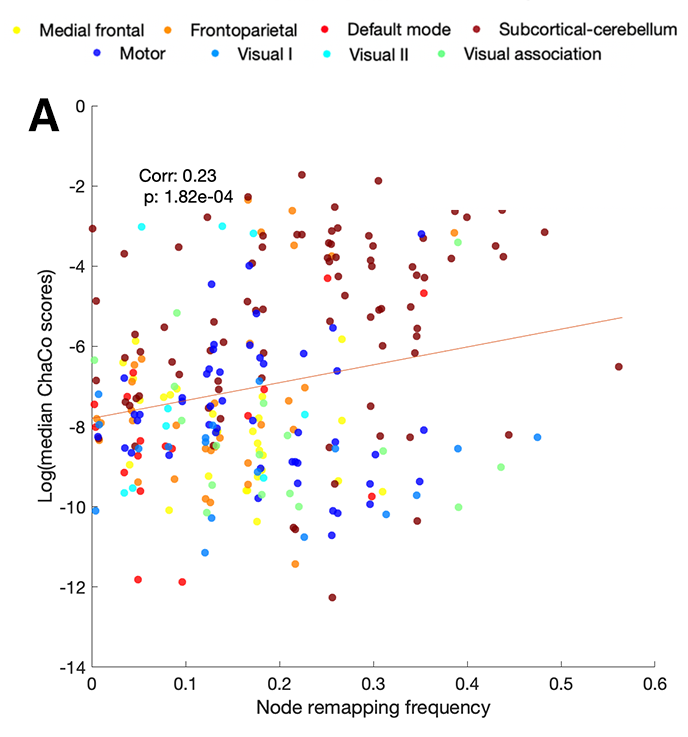
\includegraphics[width=\textwidth]{chapter1/Figure4A.png}
    \caption[]{}
\end{figure}
\null
\vfill
\clearpage
\null
\vfill
\begin{figure}[h!]
		\ContinuedFloat
		\captionsetup{labelformat=adja-page}
    \centering
    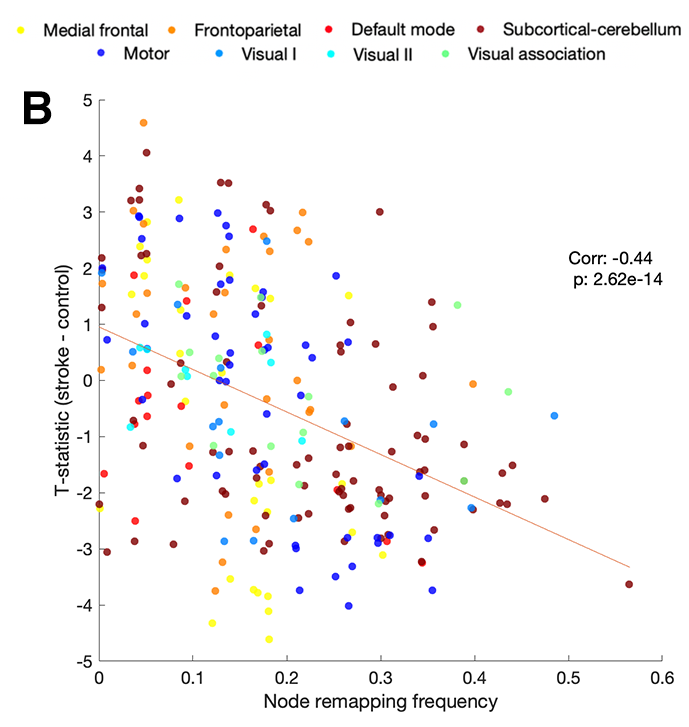
\includegraphics[width=\textwidth]{chapter1/Figure4B.png}
    \caption[]{}
\end{figure}
\null
\vfill
\clearpage
\null
\vfill
\begin{figure}[h!]
		\ContinuedFloat
		\captionsetup{labelformat=adja-page}
    \centering
    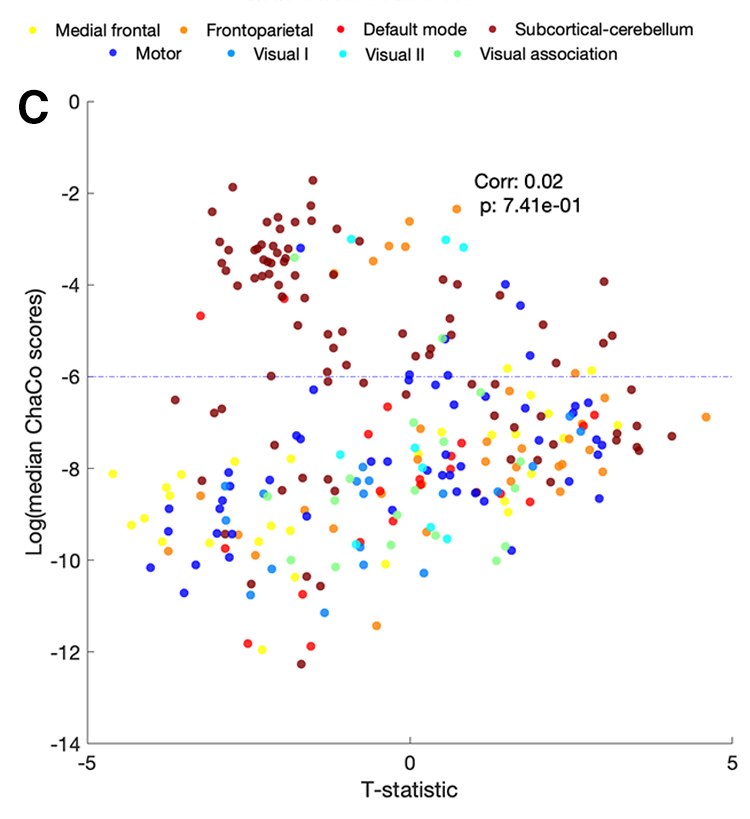
\includegraphics[width=\textwidth]{chapter1/Figure4C.png}
    \caption[]{}
\end{figure}
\null
\vfill
\clearpage
\null
\vfill
\begin{figure}[h!]
		\ContinuedFloat
		\captionsetup{labelformat=adja-page}
    \centering
    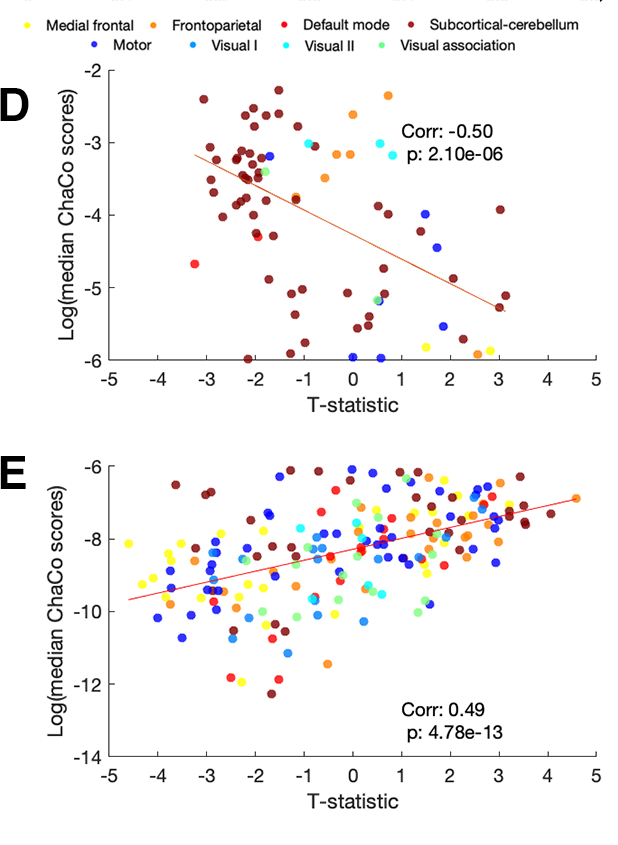
\includegraphics[width=\textwidth]{chapter1/Figure4DE.png}
    \caption[]{}
\end{figure}


    
    

	\subsection{Functional reorganization is related to impairment and recovery}
	We observed a significant positive correlation between subject-level early post-stroke remaps (between 1 weeks and 2 weeks post-stroke) and the 6 month improvement in motor scores, as measured by the difference in Fugl-Meyer scores at 6 months and 1 week post stroke (controlling for scan lengths). This result indicates that individuals with more early functional remapping had better long-term recovery (Figure \ref{Figure1_5}A). There was also a significant negative relationship between the number of early post-stroke remaps (between 1 week and 2 weeks) and baseline Fugl-Meyer scores, such that more impaired subjects had more remapping at baseline (Figure \ref{Figure1_5}B). The linear mixed effects model demonstrated a statistically significant relationship between 'remapping' and change in Fugl-Meyer score. For every one unit increase in 'remapping', there is an average increase of 0.15 units in the change in normalized Fugl-Meyer scores, holding all other factors constant (p = 0.006) (Figure \ref{Figure1_5}C). The amount of recovery between subsequent sessions was  positively associated with the number of remaps between sessions for the two comparisons between 1 week and 2 weeks post-stroke (Figure \ref{Figure1_5}D), but only a trend for significance existed at the 2 weeks to 1 month time points and there was no significant correlation for the 3 and 6 months comparison.
	


\clearpage
\null
\vfill
\begin{figure}[!hp]
\caption{Relationship between subject-level remapping, baseline motor impairment, eventual motor recovery.  }
\caption*{Subject-level remapping is related to baseline motor impairment and eventual motor recovery. \textbf{A.} Pearson correlation between subject-level remaps between 1 week and 2 weeks post stroke and change in Fugl-Meyer scores between 1 week and 6 months post-stroke. \textbf{B.} Pearson correlation between subject-level remaps between 1 week FC and 2 week FC and 1 week Fugl-Meyer scores, controlling for scan lengths at 1 week post-stroke at 2 weeks post stroke. \textbf{C.} Results from linear mixed effects analysis; each color indicates a different individuals' longitudinal time point. \textbf{D.} Pearson correlation subject-level remaps for each pair of time points and the change in Fugl-Meyer scores between time points, controlling for the scan length of the 2 scans in the remapping calculation.}
    \label{Figure1_5}
\end{figure}
\null
\vfill
\clearpage
\null
\vfill
\begin{figure}[h!]
		\ContinuedFloat
		\captionsetup{labelformat=adja-page}
    \centering
    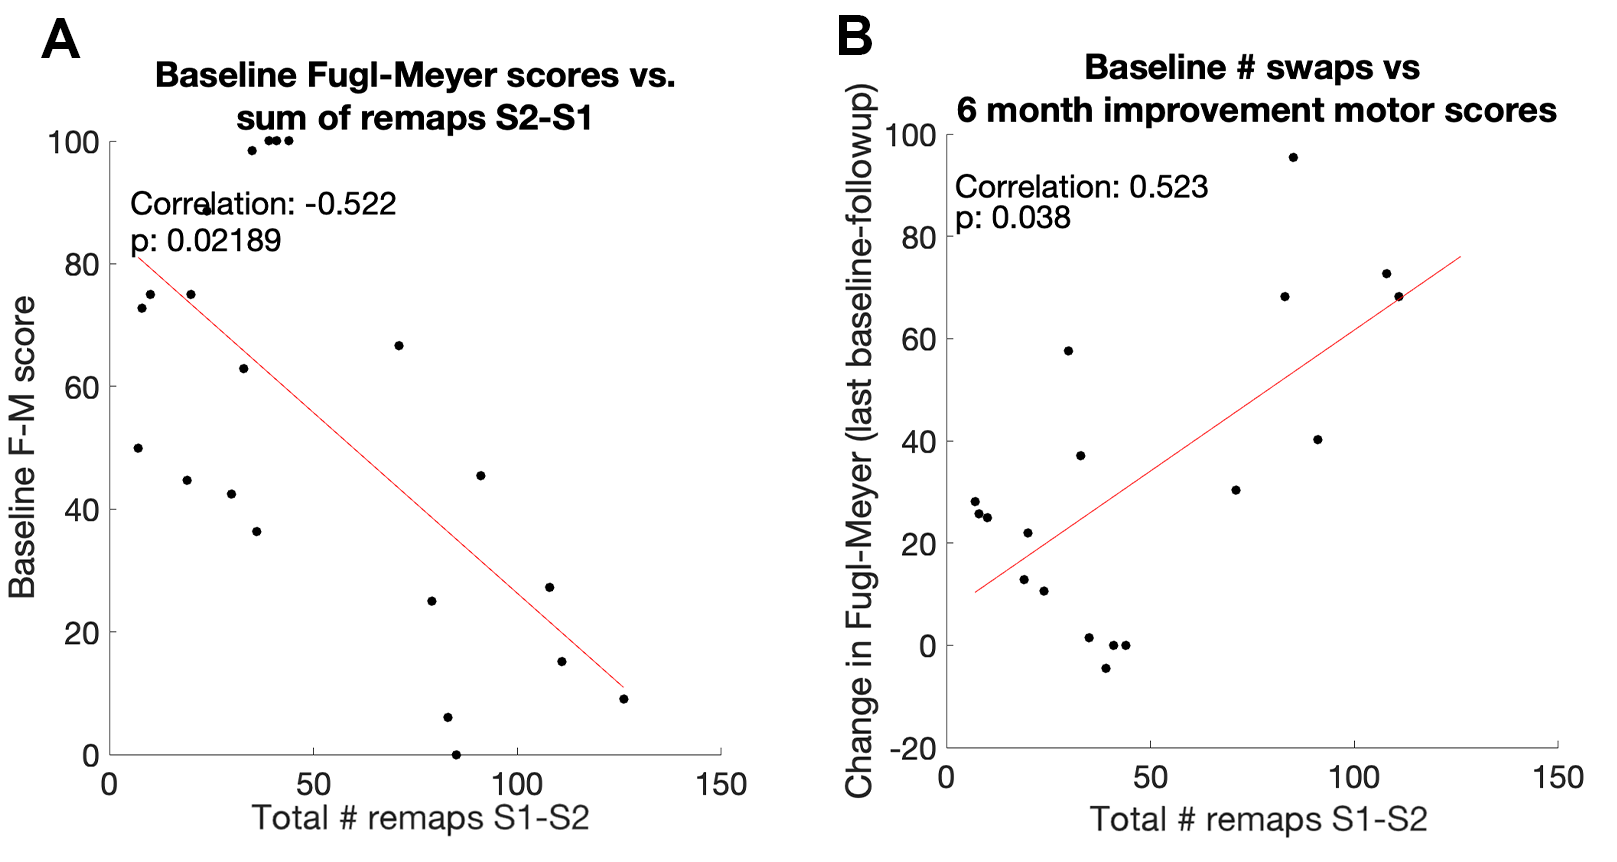
\includegraphics[width=\textwidth]{chapter1/Figure5AB.png}
    \caption[]{}
\end{figure}
\null
\vfill
\clearpage
\null
\vfill
\begin{figure}[h!]
		\ContinuedFloat
		\captionsetup{labelformat=adja-page}
    \centering
    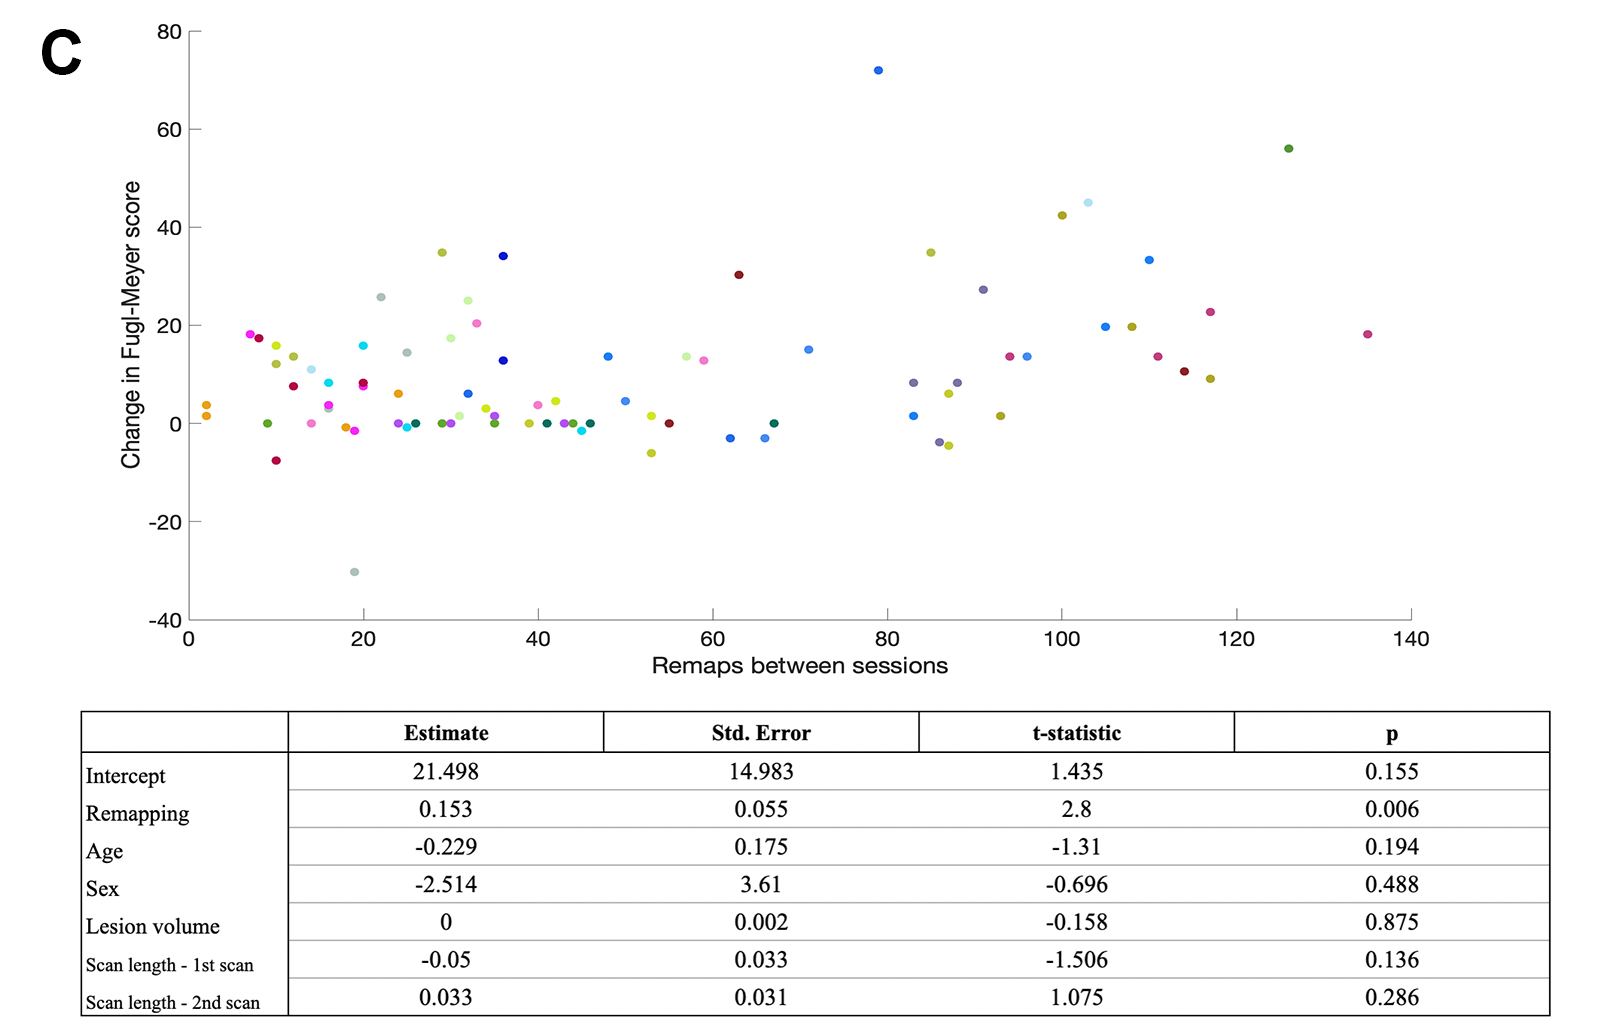
\includegraphics[width=\textwidth]{chapter1/Figure5C.png}
    \caption[]{}
\end{figure}
\null
\vfill
\clearpage
\null
\vfill
\begin{figure}[h!]
		\ContinuedFloat
		\captionsetup{labelformat=adja-page}
    \centering
    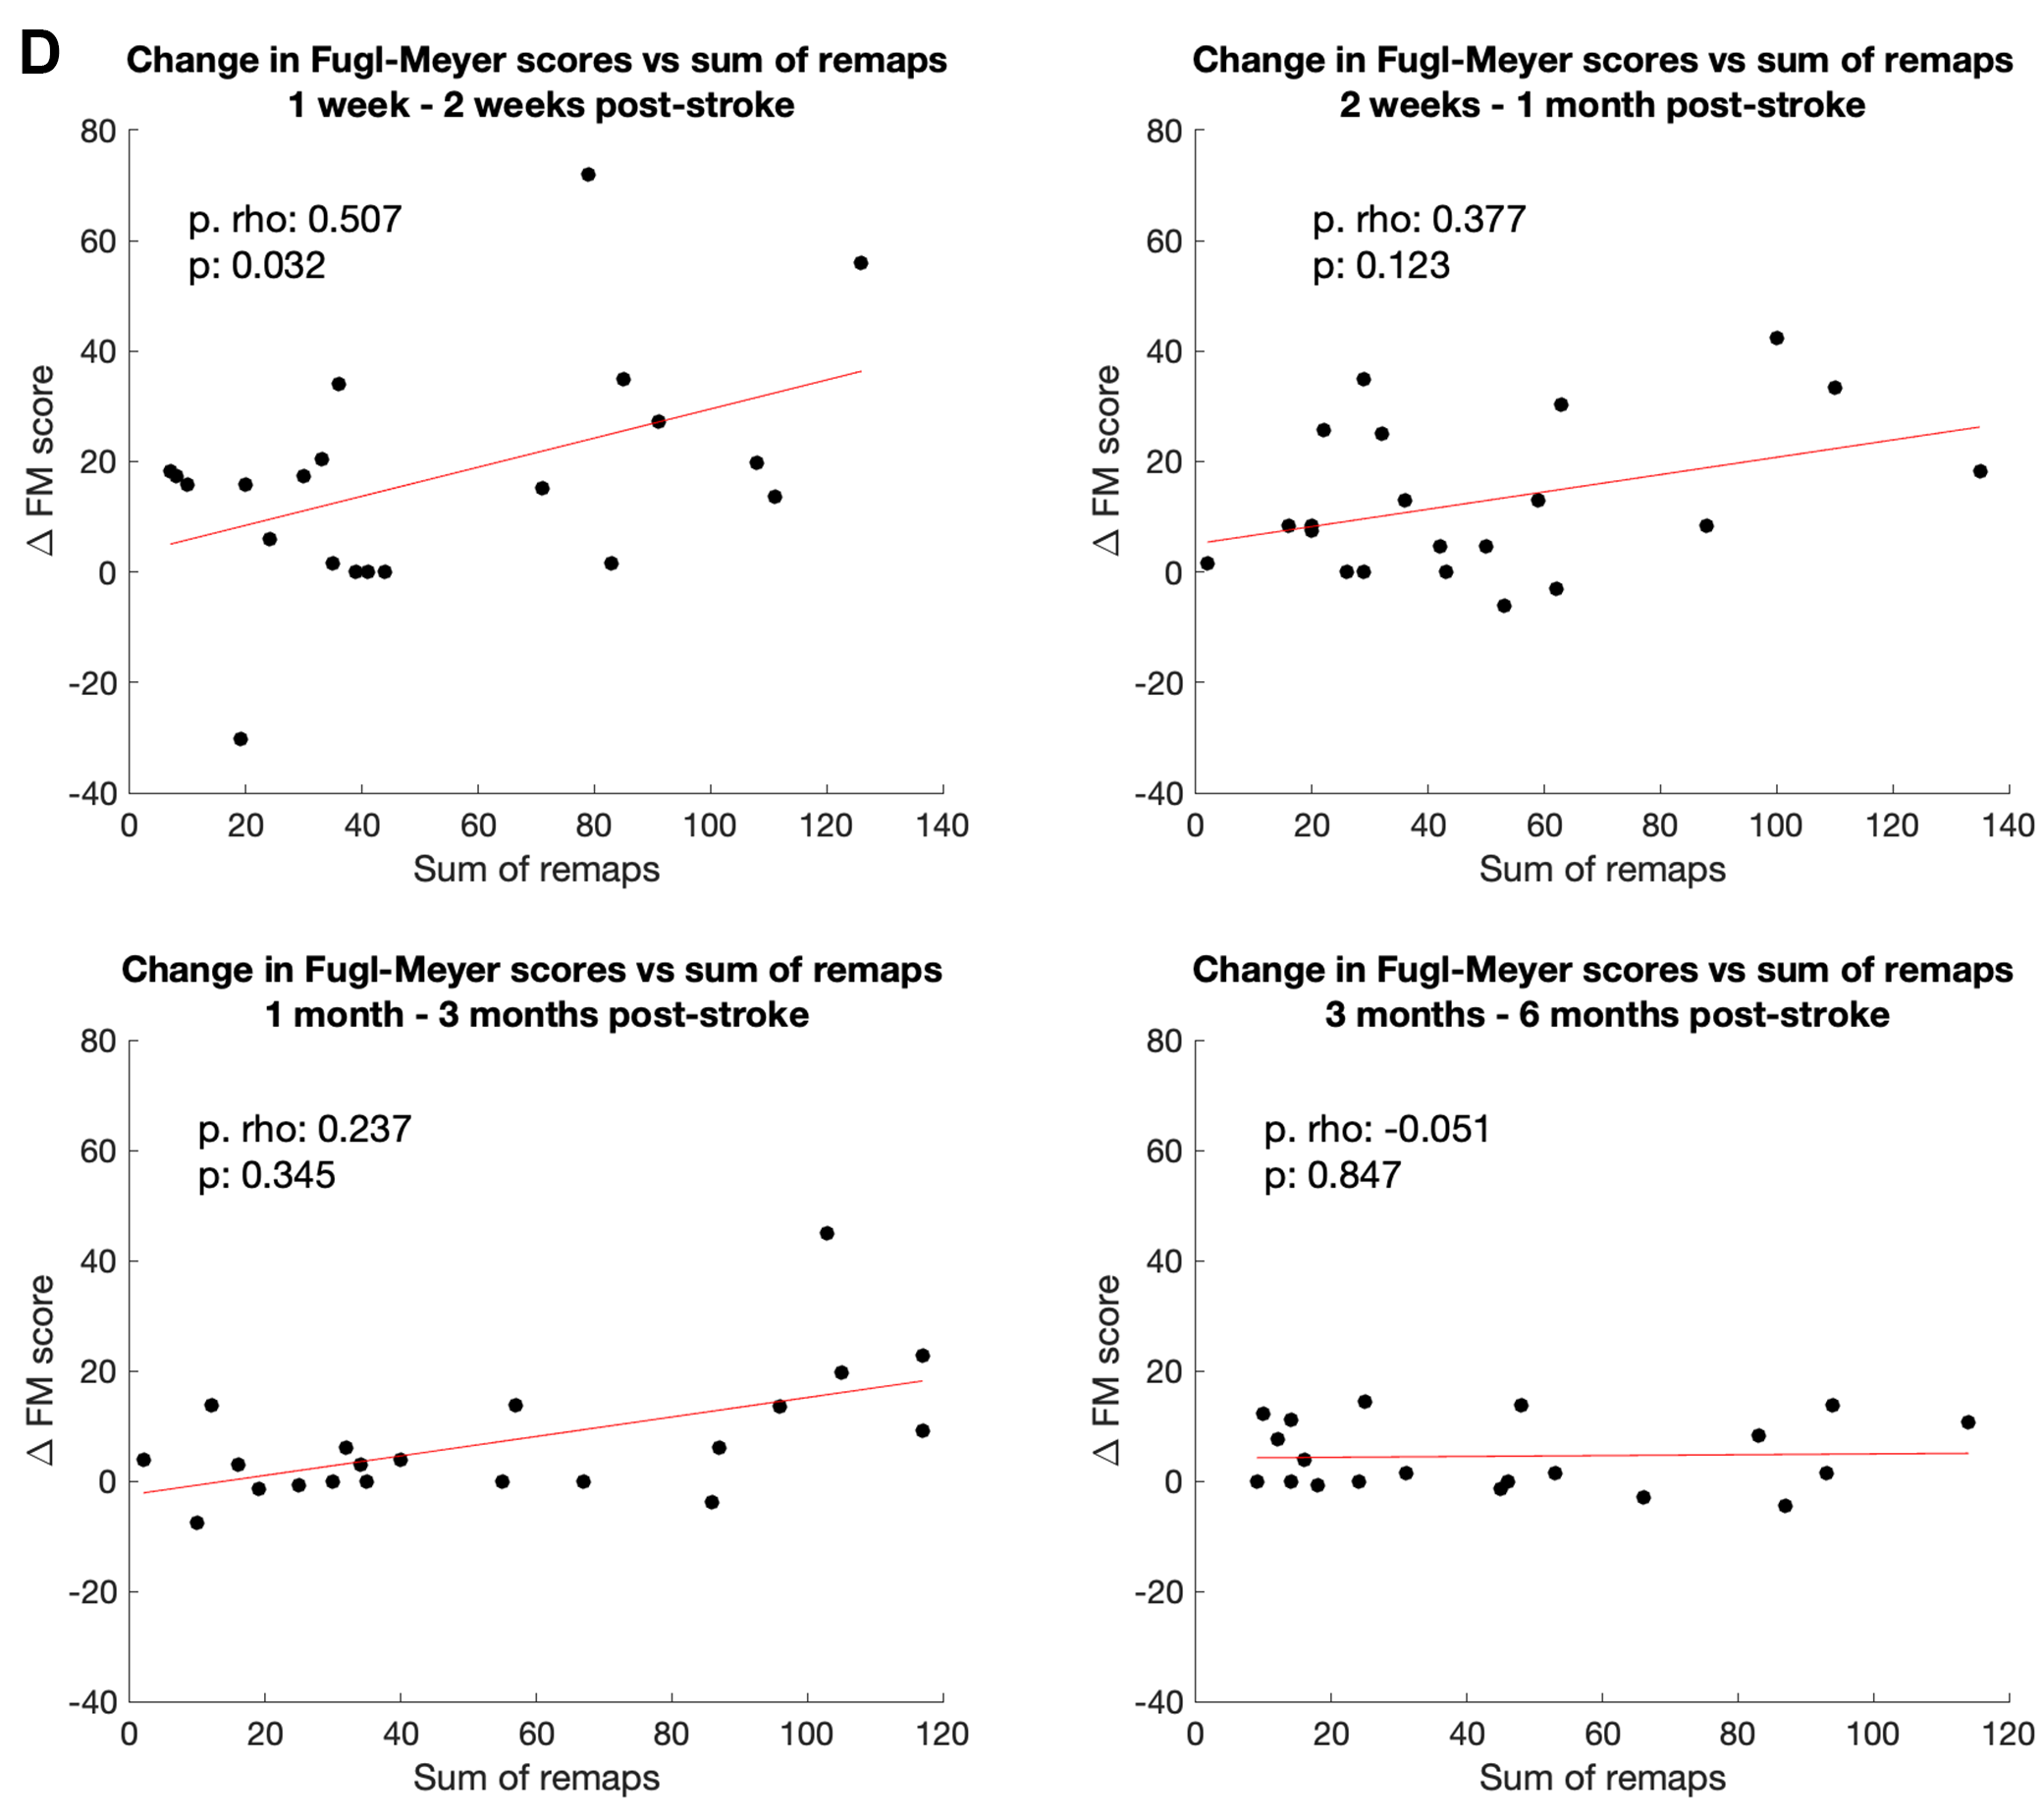
\includegraphics[width=\textwidth]{chapter1/Figure5D.png}
    \caption[]{}
\end{figure}
\null
\vfill
\clearpage
	\subsection{Robustness of results}
	The maximum overlap of lesions with each ROI is no more than 30 percent (Figure \ref{SupplementaryFigure19}). and, importantly, lesioned voxels were excluded from FC calculations. We also found that the number of remaps was not related to differences in in-scanner motion between scans, as measured by framewise displacement (Figure \ref{SupplementaryFigure20}).

\section{Discussion}
	In this paper we proposed a measure of functional connectome reorganization based on graph matching and evaluated its relationship to structural $\&$ functional disconnection and motor impairment/recovery in a set of 23 individuals with pontine stroke. We observed instances of functional reorganization over the 1 week to 6 months post-stroke period and demonstrated that the areas that undergo functional reorganization most frequently are in cerebellar/subcortical and motor networks. Furthermore, regions more impacted by stroke via disruption to their structural and functional connections had more functional remapping over time. Finally, we show that functional reorganization one week post-stroke is highly related to both baseline impairment and the extent of motor recovery at 6 months, and, finally, that the extent of functional reorganization between 1 week and 2 weeks post-stroke is correlated with the extent of motor recovery observed in this same subacute time period.
	
	We first note that remaps, defined in this paper as instances where a node is assigned to a different node longitudinally in the linear assignment algorithm, were observed in the control population. This ‘noise’ may be related to inherent variability in subject-level functional connectivity, acquisition-related noise, or a combination of both. Graph matching has recently been used to develop a measure of connectome similarity within healthy controls (\cite{Osmanlioglu2020-xz}). Consistent with our findings, Osmanlioglu and colleagues observe that graph matching using the same subject’s functional connectomes acquired during different scans is imperfect, i.e., on average there are several remaps in a single subject’s functional connectomes, suggesting that functional network structure in the same individual over time is variable. To discern the difference between natural individual variability in functional connectivity and signal, we removed all remaps that were observed in more than 5 control subjects. Almost certainly, we have not completely isolated the influence of natural individual variability; this methodology can likely be improved with future studies investigating graph matching patterns within larger populations of healthy individuals. Scan duration also influences functional connectome similarity in healthy controls, driven by the lower SNR of shorter scans. Accordingly, we observed a relationship between subject-level remaps and scan length, such that subjects with shorter scans had more remaps. To account for this influence, we included scan duration - first and second scan length - as covariates in all longitudinal analyses, but future studies should attempt to obtain consistent scan durations for all subjects.
	
    Motor recovery following stroke is supported by active functional and structural remodelling in the area bordering the stroke, including increases in excitability, increases in dendritic spine turnover, and the formation of new axonal projections (\cite{Murphy2009-ez}). This remodelling can entail surviving cortical areas remapping functionally to compensate for post-stroke impairment (\cite{Brown2009-jn}). The dynamic reorganization of resting-state functional connectivity, observed in this stroke cohort in subcortical and cerebellar areas, may reflect longitudinal compensatory changes in representations of motor functions. Interestingly, we showed correlations between amount of functional remapping and amount of motor improvement but only in the period of time in which most post-stroke recovery occurs (within 3 months after stroke) (\cite{Lee2015-nn}). However, resting-state functional connectivity may not be fully representative of brain activation patterns underlying specific behaviors (i.e. during a task), and has shown to be constrained by the structural connectome (\cite{Kuceyeski2019-gt, Honey2009-xb}). Thus, it is possible that the remapping observed is not a functional remapping per se (in the sense of remapping a region's role in a specific task), but a shift in balance of a brain area's functional connectivity profile at rest, which could reflect task-based functional compensations, changes in network topology, and/or underlying structural remodelling. 

	We now understand that deficits arising from stroke are not only related to the damage inflicted at the stroke core, but also to remote cortical areas structurally connected to the lesion, due to retro- and anterograde degeneration (\cite{Guggisberg2019-lj}). For instance, several studies have shown that there are local reductions in cortical thickness in areas directly connected to subcortical lesions (\cite{Duering2015-iv, Cheng2015-jq}). These degenerative changes are long-term effects of a stroke. We showed that structural disconnection from a stroke lesion is associated with remapping even at 6 months post-stroke, suggesting that late-stage impacts of the stroke may trigger functional reorganization. 
    
    However, as stated earlier, recovery-related reorganization usually occurs within the first three months post-stroke. We observed recovery-related remapping primarily in the acute period (1-2 weeks after stroke), where there was also a significant correlation between structural connectome disruption and remapping as well as functional connectome disruption and remapping. Structural connectivity disruption between nodes has been linked to perturbations of functional connectivity (FC) within the first 2-4 weeks after stroke (\cite{Griffis2019-cy, Griffis2020-hx, Wodeyar2020-kz}), including by Lu and colleagues (2011), who demonstrated that pontine strokes disrupt FC between the cortex and the cerebellum. These papers generally show that damage to structural connections between nodes, direct or indirect, is associated with reductions in FC between those nodes. We observed that remapping more frequently occurs in nodes with greater structural and functional connectivity disruption due to the stroke. We observed that functional connectivity changes were related to structural connectivity disruption magnitude; nodes with more structural connectivity disruption had a negative relationship with changes in node strength, where more SC disruption was related to weaker FC. These nodes, overwhelmingly a part of the subcortical/cerebellum network, also have the highest levels of remapping. On the other hand, regions with lower structural connectivity disruption have a positive relationship with changes in node strength, where less SC disruption is associated with higher node strength. This result suggests that remapping after pontine stroke may be a mechanism that occurs to only the most severely disrupted brain regions, whose structural connections have been damaged to the point of weakened FC, whereas regions with less structural disruption can compensate for the damage in the form of upregulated FC. 
    
    Pontine strokes primarily affect large-diameter projection fibers, which tend to produce more severe functional connectivity deficits when damaged (\cite{Griffis2020-hx}). Brain regions that were once structurally and functionally connected via. these fibers may remap more often as their role in the network is taken over by other nodes with more preserved structural connections. For instance, \cite{Lu2011-ow} demonstrated reduced FC between the motor cortex and cerebellum in subjects whose cortico-ponto-cerebellar fibers were damaged from pontine stroke. Regions in the cerebellum and motor cortex that can no longer communicate via. these fibers may remap to other nodes with preserved cortical/cerebellum connectivity.
    
     Other factors may make regions more or less amenable to remapping; perhaps a region is better positioned within the network to assume lost functionality, such as in the cerebellum where there is considerable redundancy in the somatotopic layout (\cite{Mottolese2013-sd}) which may enable it to compensate more easily for lost functionality.
    
    We also show that more remapping between sessions is associated with better motor recovery between those same sessions, and that more remapping in the early phase of stroke is related to both amount of baseline impairment and the degree of motor recovery at 6 months. Functional reorganization measured with this remapping technique may be interpreted as reflecting a compensatory, beneficial process that is proportional to the extent of motor recovery. On the other hand, this approach may also be capturing phenomena that occurs during the first 6 months after stroke that are unrelated to recovered functionality, but that correlate with measures of recovery nonetheless. For instance, stroke-related increases in noise in the subcortical/cerebellum network may result in more remapping which could be the result of a random or pathological process concomitant with a recovery mechanism. Thus, more densely-sampled fMRI studies should be performed to identify other elements of this reorganization process. 
        
    The most remaps were observed in the subcortical/cerebellum network, suggesting that remapping is likely reflecting a process of functional reorganization that is spatially constrained (Figure \ref{remaps_summary}). This network-level reorganization is consistent with prior task-based studies showing remapping of motor-based activations to premotor and homologous areas, and with studies of resting-state FC that demonstrate specific spatial patterns of FC changes after stroke, like changes in resting state FC within motor networks (\cite{Zhang2016-vg}), and contralesional functional connectivity changes that are concentrated in a small set of brain regions (\cite{Yourganov2021-hd}).
     
	
	\subsection{Limitations}
	There are several limitations to this study. The first is sample size, which is partially mediated by the frequency of the longitudinal sampling and the homogeneity of the population. The second is that the impact of fMRI noise in the remapping procedure cannot be completely accounted for. We do see that some nodes with high frequency remapping are also those that have lower SNR in the fMRI data; generally, the SNR of fMRI is lowest in medial structures such as the thalamus, cortical midsurface, and most consequentially to this study, the cerebellum. Thus, it is possible that noise contamination was captured in the graph matching procedure and has leaked into the results. Our approach of using the arguably more noisy control data to filter this potential source of noise helped mitigate this drawback. Second, structural disconnection metrics were obtained for each individual using indirect methods (i.e. the Network Modification Tool), instead of directly from diffusion MRI in the individuals with stroke. Third, the correlation between baseline and long-term recovery in stroke subjects is generally high (\cite{Krakauer2015-sy}); because of the small sample size in this study, it is not possible to discern whether the relationship between early remapping and 6 month recovery holds while controlling for initial impairment. Fourth, we did not have data available regarding the rehabilitation program, as it was not collected at the time of fMRI scanning and motor assessments, so the effect of rehabilitation could not be accounted for. 

\section{Conclusion}
	In this study we proposed a measure of functional connectome reorganization, called remapping, and applied it to longitudinal resting-state fMRI data in a cohort of pontine stroke patients. Remapping was observed in all stroke subjects and was correlated with recovery over the early to late subacute phases. Areas impacted by the lesion through structural disconnection were more likely to remap than those areas not impacted by the lesion. This work expands our understanding of functional processes related to recovery after stroke, and future studies should examine remapping in other populations beyond pontine stroke subjects, such as those with cortical stroke. If we can identify subjects who have more potential for functional reorganization, or can devise therapeutics to boost this remapping mechanism, we may be able to improve patient outcomes after stroke.
	
\label{chap:1}

\chapter{Frontoparietal network activation is associated with motor recovery in ischemic stroke patients*}
\blfootnote{* Olafson, E., Russello, G., Jamison, K. W., Liu, H., Wang, D., Bruss, J. E., Boes, A. D.,  Kuceyeski, A. (2022). Frontoparietal network activation is associated with motor recovery in ischemic stroke patients. Communications Biology, 5(1), 993.}
\section{Introduction}
	The ability to perform motor functions after stroke depends on the coordinated reconfiguration of distinct global brain activity patterns (\cite{Park2011-kx}). Novel data-driven techniques to characterize whole-brain activity in functional magnetic resonance imaging (fMRI) scans at single-frame resolutions have illuminated the dynamic nature of brain activity in several brain disorders (\cite{ Braun2021-iy, Adhikari2020-tk, Kaiser2019-rf}), but methods assigning each time point to a discrete state have not yet been applied to examine altered brain dynamics in stroke patients. These methods provide information about brain function complementary to and beyond traditional static measures of functional connectivity (\cite{Cornblath2020-nc}), and thus may provide new insights regarding the process of recovery following stroke.
	
	Prior work characterizing spatiotemporal brain dynamics after stroke has focused on identifying altered functional connectivity states, which reflect time-varying patterns of functional connectivity (FC). Dynamic FC analyses identify recurrent connectivity patterns using a sliding window approach, in which FC is repeatedly calculated over consecutive windowed segments of the fMRI scan. This approach yields FC networks that fluctuate over time, with a temporal resolution proportional to the size of the window; about 30-60 seconds (\cite{Savva2019-hk}). In stroke populations, dynamic FC studies have demonstrated stroke-related differences in temporal configurations of motor networks (\cite{Bonkhoff2020-bx}) and participation in connectivity states that varies with severity (\cite{Bonkhoff2020-de}). 
	
	In contrast, analysis at a single relaxation time (TR) resolution of activation states identified in a data-driven fashion using k-means clustering of the time series data (\cite{Cornblath2020-nc}) provides a closer look at the moment-to-moment changes in recurrent brain activity, with the time spent in each state lasting, on average, 5-10 seconds (\cite{Cornblath2020-nc}). A benefit to analysing brain activation states over or alongside connectivity states is that activation patterns can enable a more refined interpretation of connectivity differences between groups. FC is traditionally defined as the correlation between two brain region's activity over time. FC may be driven by two distinct features of brain activity: by the individualized spatial patterns of large-amplitude activations (\cite{Zamani_Esfahlani2020-dn}), and by the amount of time spent in recurring patterns of activity (\cite{Betzel2021-ve, Baker2014-zt}). In this paper we aim to identify group-level patterns of brain activity after stroke that relate to recovery, and assume that recurring activity patterns are shared across individuals but are expressed in different proportions.   Understanding the temporal patterns of activity underlying recovery-relevant FC changes after stroke can aid in the development of more accurate targets in stimulation therapies.
	
     Recent work has highlighted the importance of frontoparietal areas in supporting motor abilities in the chronic phase of stroke (\cite{Tscherpel2020-oi, Hensel2022-sl}) specifically in patients with poor corticospinal tract (CST) integrity (\cite{Hordacre2021-ct}). When these descending motor pathways are significantly damaged, descending white matter tracts from higher-order motor areas, like regions of the frontoparietal network (FPN), may support motor output. Because of the differential use of the dominant and non-dominant arm throughout life, we were interested in determining whether handedness relative to the lesioned hemisphere would modify the recruitment of a frontoparietal state to promote motor recovery. Understanding this type of subject- and lesion-specific variability in the post-stroke recovery process is precisely the type of information needed to develop personalized rehabilitation strategies to maximally promote recovery.
  
	Here, we propose to first identify and characterize recurring brain activity patterns, or states, in healthy controls and individuals with ischemic pontine stroke (\cite{Cornblath2020-nc}). We hypothesized that individuals with ischemic stroke would display altered dynamic brain state metrics, e.g. fractional occupancy, dwell time and appearance rates, compared to control subjects, and, further, that these dynamic state metrics would be associated with measures of motor recovery. In an exploratory analysis, we examined whether time spent in a brain state characterized by frontoparietal activation would be differentially recruited for later-stage motor recovery depending on the side of the lesion relative to the subject's handedness. Finally, to bridge dynamic brain state analyses and more classic functional connectivity approaches, we assessed the relationship between the amount of time spent in different brain states and the FC between several resting-state networks. This last analysis is particularly important in terms of linking our current findings to previous studies of how rehabilitation techniques, including non-invasive brain stimulation, modulate the functional connectome and possibly motor recovery.
	
	\begin{figure}
	\centering
	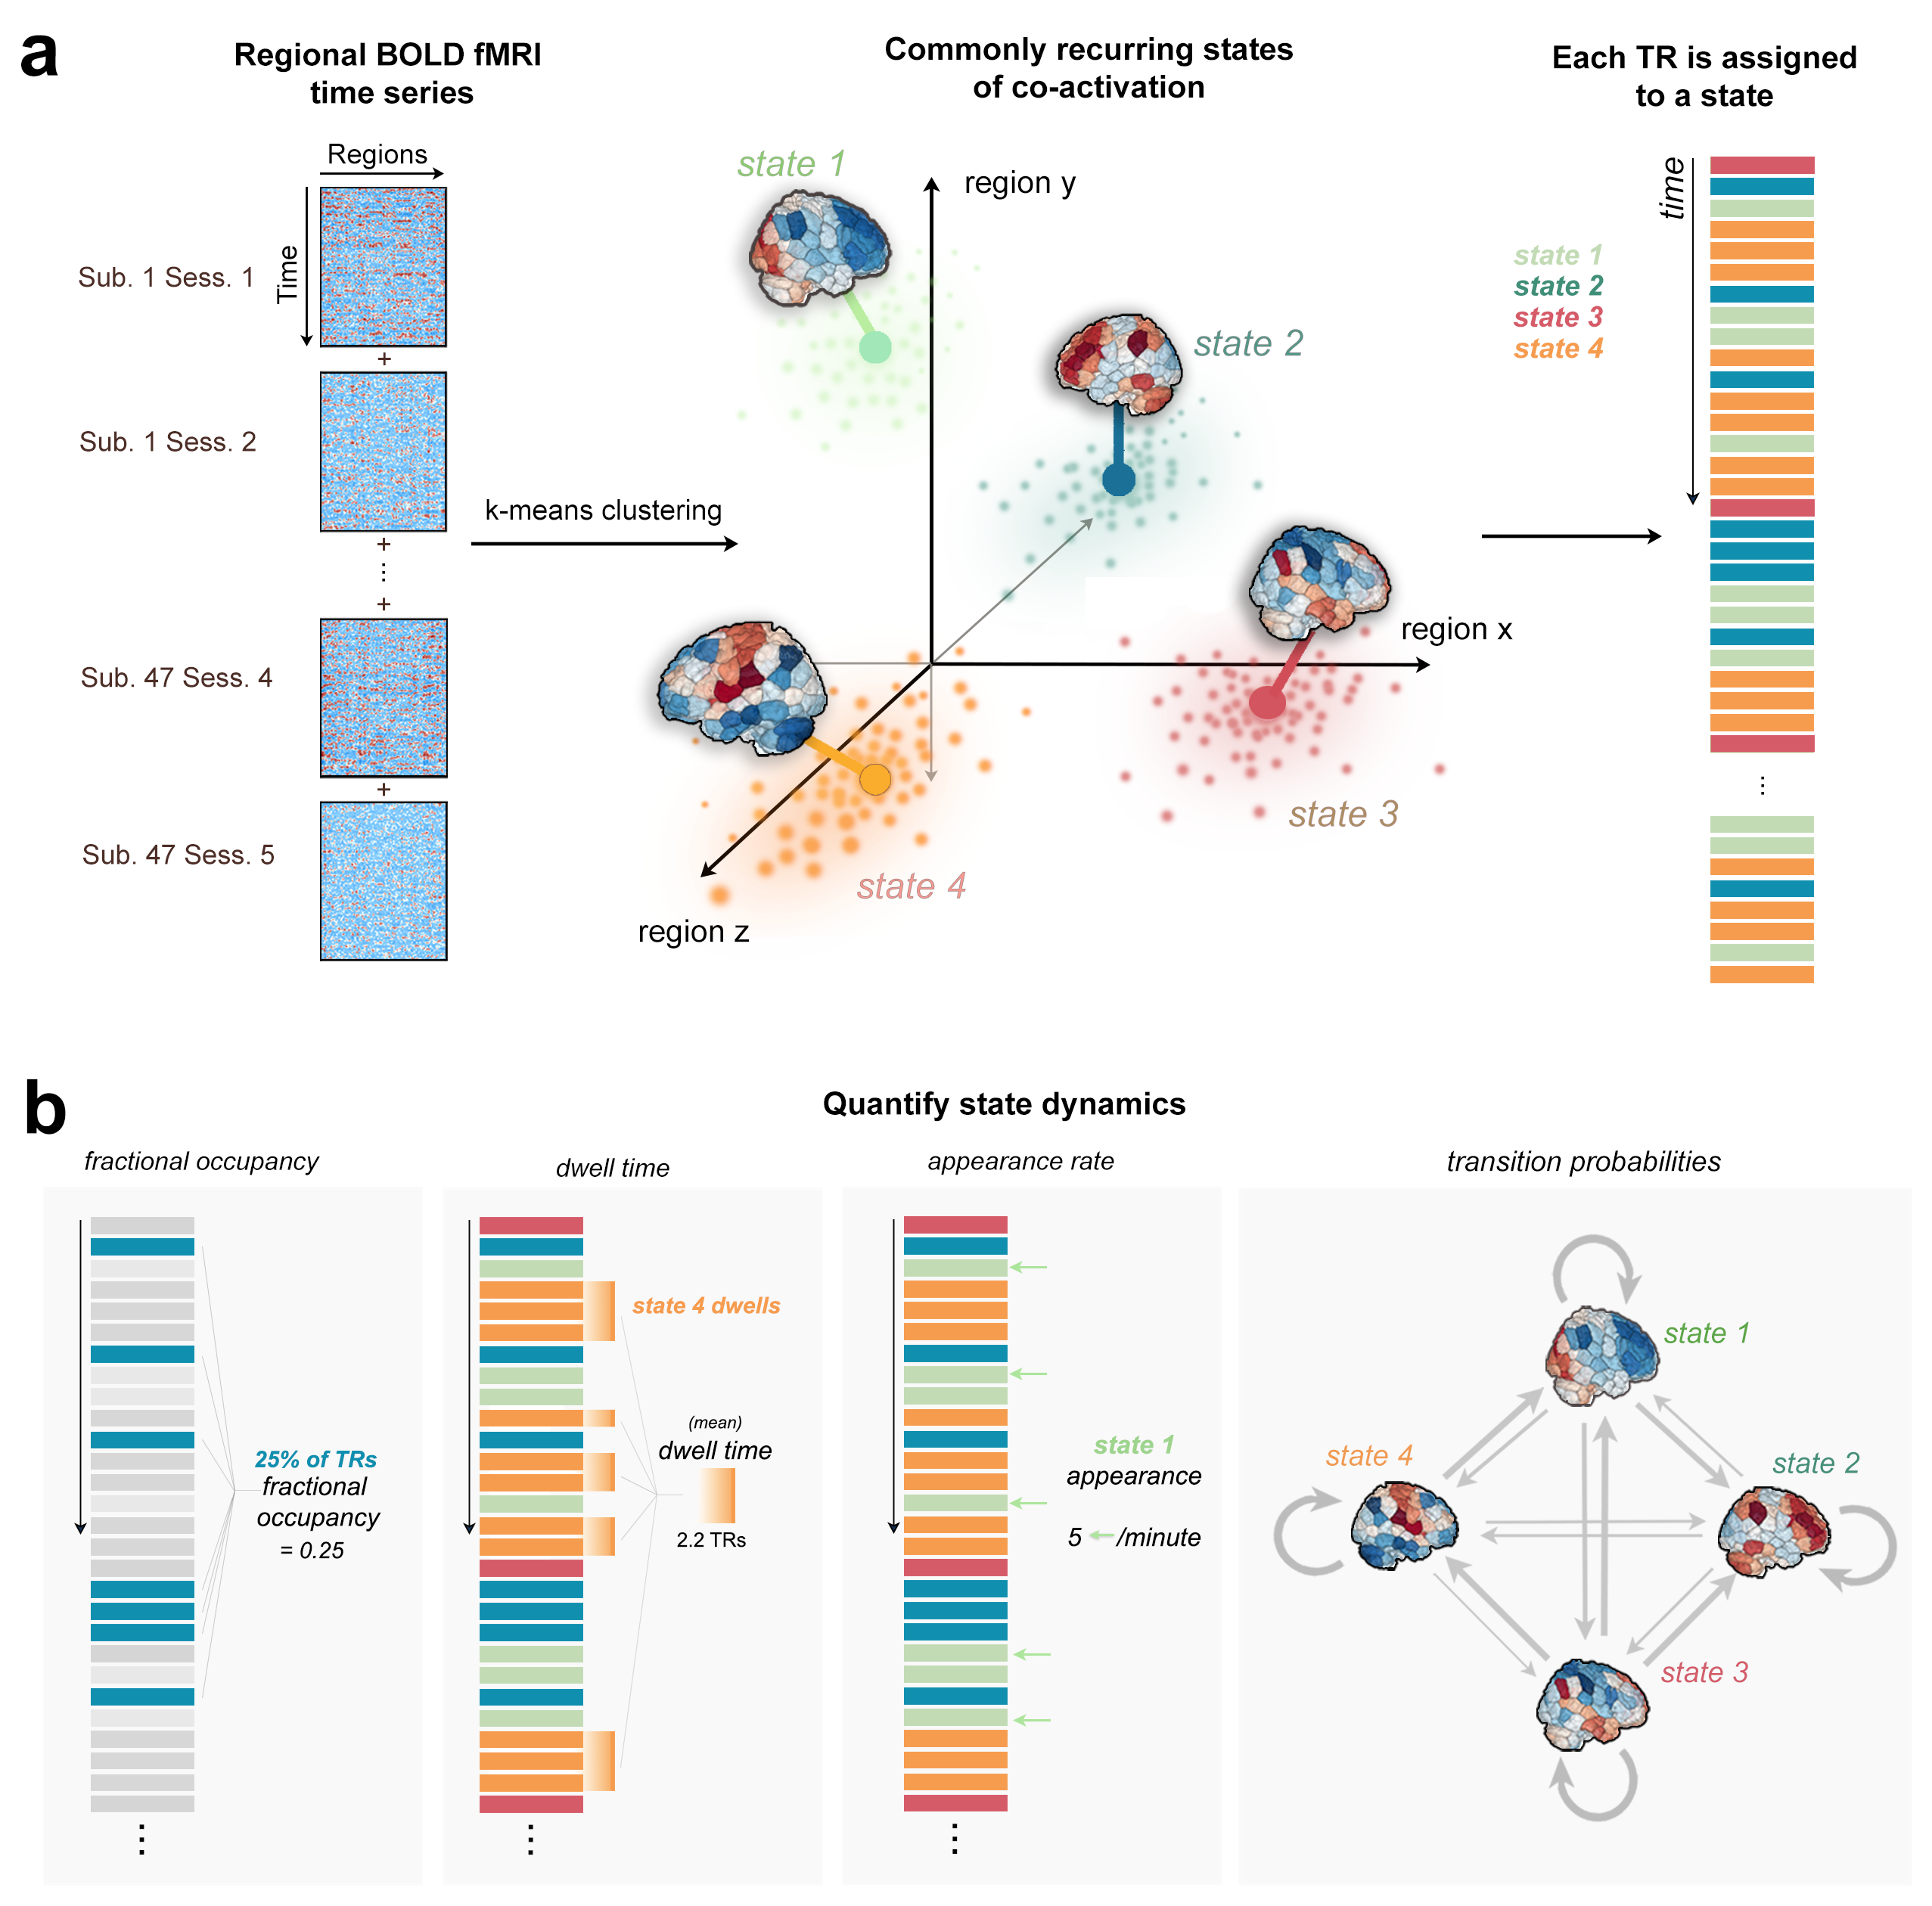
\includegraphics[width=1\linewidth]{chapter2/Figure1.png}
	\caption{Clustering of time series data and quantification of dynamic state metrics. \textbf{a}. Time series data from all subjects were concatenated together along the time dimension. K-means clustering produced 4 distinct brain activation states defined by different locations in regional activation space (image adapted from \cite{Cornblath2020-nc}). Each TR is assigned to one of four brain states based on k-means partitions. \textbf{b}. Fractional occupancy, dwell time, appearance rate, and transition probabilities are calculated separately for each subject and for each state.  }
	\label{Figure2_1}
    \end{figure}
    
\section{Methods}
	\subsection*{Data description}
	 The data consist of 23 first-episode stroke patients (34-74 years old; mean age 57 years; 8 female) with isolated pontine infarcts and 24 healthy sex-matched controls (33-65 years old; mean age 52 years; 10 female). A subset of the data (11 stroke subjects and 11 healthy control subjects) used here has been previously described in \cite{Lu2011-ow}; the current study includes an additional 12 stroke subjects and 13 control subjects. Of the twenty-three stroke subjects, fourteen had right brainstem infarcts and nine had left brainstem infarcts (Supplementary Figure 1a, 2, 3). Written informed consent was obtained from all participants. Patients were scanned between two and five times over a period of 6 months. Specifically, MRIs were obtained at 7, 14, 30, 90 and 180 days after stroke onset on a 3T TimTrio Siemens using a 12-channel phase-array head coil. Fugl-Meyer assessments were performed twice for each subject at each session and averaged (Supplementary Figure 1b). The Fugl-Meyer test includes 33 tasks that assesses motor function, balance, sensation, and joint function of the upper limbs (\cite{Fugl-Meyer1975-nh}). Each task was rated on a scale of 0 to 2 (0 indicates the subject was unable to perform the task, 1 indicates the subject could partially perform the task, and 2 indicates the subject was able to perform the task). The total sum of the 33 scores was then normalized to a score between 0 and 100, where 100 represents the best possible performance across all 33 tasks. Anatomical images were acquired using a sagittal MP-RAGE three-dimensional T1-weighed sequence (TR, 1600ms; TE 2.15ms; flip angle, 9°, 1.0 mm isotropic voxels, FOV 256 x 256). Each MRI session involved between two and four runs of task-free fMRI at 6 minutes each. Subjects were instructed to stay awake with their eyes open; no other task instruction was provided. Images were acquired using the gradient-echo echo-planar pulse sequence (TR, 3000ms; TE, 30ms; flip angle, 90°, 3 mm isotropic voxels). Anatomical MRI, lesion masks and fMRI data were processed as described below and in (\cite{Olafson2021-qt}).
	 
 
    	 
	\subsection*{Anatomical MRI processing}
	Preprocessing of the longitudinal anatomical MRIs included affine registration of each subject’s T1 scans to the baseline T1 scan, collapsing co-registered files to an average T1 and creation of a skull-stripped brain mask followed by manual editing and binarization of the hand-edited mask. The brain mask was then transformed back to each of the follow-up T1s in native space using the inverse registration acquired from the first step. This was followed by bias field correction of all the T1 scans, transformation of native-space bias field-corrected data back to baseline space, and the creation of an average bias field-corrected scan for each subject. Stroke lesion masks were hand-drawn on these transformed T1 scans by ADB and JEB. Structural normalization was performed with the ANTs toolbox (\cite{Avants2011-bl}).
	
	\subsection*{Functional MRI processing}
	Preprocessing of the longitudinal functional MRIs was performed using the CONN toolbox (\cite{Whitfield-Gabrieli2012-ox}), including functional realignment of volumes to the baseline volume, slice timing correction for alternating acquisition, segmentation and normalization, and smoothing with a 4 mm FWHM kernel. This was followed by a denoising protocol (CompCor) (\cite{Behzadi2007-zt}) which regressed out the cerebrospinal fluid and white matter signal, as well as 24 realignment parameters (added first-order derivatives and quadratic effects). Temporal band-pass filtering (0.008 - 0.09 Hz), despiking and global signal removal regression were also performed. The first four frames of each BOLD run were removed. Frame censoring was applied to scans with a framewise displacement threshold of 0.5 mm along with its preceding scan (\cite{Power2012-zm}). Regional time series were acquired by parcellating the scans into 268 non-overlapping brain regions using a functional atlas derived from healthy controls (\cite{Shen2013-zn}) and averaging the time course of all voxels within a given region. Voxels identified as lesioned were excluded from regional time series calculations. The first 200 volumes from each subject's fMRI were used for subsequent analyses to ensure equal contribution of each scan to the brain state clustering (see below for details). Finally, each of 268 regions was assigned to one of 8 functional networks, identified by (\cite{Finn2015-er}) using spectral clustering in healthy subjects (Supplementary Figure 4) named as follows: medial frontal network, frontoparietal network, default mode network, subcortical/cerebellum network, motor network, visual I network, visual II network, and the visual association network. These networks reflect collections of brain regions whose temporal signals are homogeneous at rest (i.e., the activity of regions within each network is similar over time) in a healthy population, and are referred to as canonical networks due to their repeated observation in resting-state data.
	
	\subsection*{Dynamic brain states and their metrics}
	 Following Cornblath et al. (2020), all subjects’ regional fMRI time series were concatenated, producing an n x p matrix where n = 47 subjects * 200 TRs * 2-5 sessions and p = 268 brain regions). This matrix was z-scored along columns such that each brain region had a mean of 0 and a standard deviation of 1. K-means clustering was then applied to identify clusters of brain activation patterns, or states (Figure \ref{Figure1}a). Pearson correlation was used as the cluster distance metric and clustering was repeated 50 times with different random initializations before choosing the solution with the best separation of the data (minimum sum of point-to-centroid distances, summed over all k clusters). To determine the optimal number of clusters and evaluate the quality of clustering, we performed several analyses (Supplementary Figure 5). First, we plotted the variance explained by clustering (between-cluster variance divided by the sum of between-cluster and within-cluster variance) for k = 2 to 12 and identified the curve's elbow at k = 4 as a potential optimal number of clusters. We also plotted the distortion curve, which is the average distance from each point to its centroid and again determined via elbow criteria an optimal cluster number of 4. We then plotted silhouette coefficients for k = 4 to assess if there was evidence of misassignment of any of the points. To further assess the stability of clustering and ensure our partitions were reliable at k = 4, we repeated the above clustering process 50 times and compared the adjusted mutual information (AMI) between each of the 50 results. The partition which shared the greatest total AMI with all other partitions was selected as the final cluster assignment. The centroids of each state (cluster) were calculated by taking the mean of all TRs assigned to that state in regional activation space (\cite{Cornblath2020-nc}). Following Cornblath et al., dominant networks in each state were determined by calculating the cosine similarity between each of 8  networks and each centroid. High and low amplitude network-level activations were assessed separately by taking the cosine similarity of the positive and negative parts of the centroid (and zeroing out values with the opposite sign), respectively. 
	 
	 We performed several analyses to assess the robustness of our results under different conditions. First, we repeated the entire clustering process using two other brain atlases of varying resolutions: the group average FreeSurfer Desikan-Killany atlas with additional cerebellum and subcortical regions (86 regions) (\cite{Desikan2006-vf}) and the CC400 atlas (400 regions) (\cite{Craddock2012-kl}). Finally, we performed the clustering after combining stroke and control data together because we were interested in determining differences in shared activation states across both groups. However, it may be possible that stroke and control subjects occupy distinct states that can only be observed by clustering stroke and control subjects separately. Therefore, we repeated the clustering on the stroke and control subject data separately to determine if there were any differences in the resulting states compared to those obtained with the combined data.

	 


	 FO, DT, AR and TPs were calculated separately for each of the 5 sessions (1 week, 2 weeks, 1 month, 3 months, and 6 months post baseline or stroke) and the average FO/DT/AR/TPs for each subject was obtained by taking the mean across their longitudinal sessions. State dynamics metrics were compared between groups using unpaired two-tailed t-tests and corrected for multiple comparisons using Benjamini-Hochberg (BH) and false discovery rate (FDR) of 0.05 (\cite{Benjamini1995-bb}). 

	 \subsection*{Assessment of corticospinal tract integrity}
	 The probabilistic Tang brainstem atlas (\cite{Tang2018-ac}) was used to define left and right binary CST masks in 2mm MNI space by voxel-wise thresholding at 50$\%$. The Dice overlap between the left and right CST masks and the binarized lesion mask was calculated for each subject and lesions were visualized to verify intersection with the CST (Supplementary Figure 2 and 3). In one subject (SUB13), Dice overlap with CSTs were low; however, upon visualization the lesion appeared to impact CST ventral to the atlas, i.e. in the spinal cord. This was confirmed by assessing the lesion's overlap with a spinal cord atlas (Supplementary Figure 12) using the Spinal Cord Toolbox (\cite{De_Leener2017-ev}). In total, 21/23 subjects had CST damage and 10/23 subjects had damage to their dominant-hand CST, but only 9/23 had motor assessment data at the 3- and/or 6-month time points. Of the 9 subjects with dominant CST damage and motor scores, 7/23 were right-handed and either had left CST damage superior to decussation or right spinal cord CST damage inferior to decussation, 1/23 was left-handed with bilateral damage, and 1/23 was left-handed with right CST damage (Supplementary Table 1).
	 
	 \subsection*{Relating $FPN^+$ state metrics to chronic motor  outcomes}
     We were interested in determining whether \begin{Large}$FPN^+$\end{Large} state metrics related to longer-term (chronic) motor performance outcomes specifically in subjects with dominant hemisphere CST damage. To assess the interaction effect of hand dominance on the relationship between the frontoparietal state parameters (FO and DT) over time and Fugl-Meyer (FM) scores over time, two linear models were constructed:

     \begin{center}
      \begin{Large}
	 \begin{equation}
	    \Delta FM_{chronic} \sim  CST_D + \Delta DT^{FPN^+}_{chronic} + CST_D*\Delta DT^{FPN^+}_{chronic} + \beta
	\end{equation} 

	 \begin{equation}
	    \Delta FM_{chronic} \sim  CST_D + \Delta FO^{FPN^+}_{chronic} + CST_D*\Delta FO^{FPN^+}_{chronic} + \beta  
	\end{equation}
		\end{Large}
	\end{center}

	Where:
	
	 \begin{Large}
	\begin{center}

	\begin{equation}
	    \Delta FM_{chronic}  = FM_{chronic - FM_{baseline}} 
	\end{equation}

	\begin{equation}
	    \Delta DT^{FPN^+}_{chronic}  = DT^{FPN^+}_{chronic}-DT^{FPN^+}_{baseline} 
	\end{equation}

	\begin{equation}
	    \Delta FO^{FPN^+}_{chronic}  = FO^{FPN^+}_{chronic}-FO^{FPN^+}_{baseline} 
	\end{equation}
	\end{center}
\end{Large}
	and \begin{Large}$CST_D$\end{Large} is a binary variable indicating whether the subject's dominant-hand CST had non-zero Dice overlap with the lesion.  \begin{Large}$FM_{baseline}$\end{Large} was set to the earliest $FM$ score available for each subject, which was the FM score at 1 week post-stroke for most of the subjects. For two subjects (SUB22 and SUB23), 1 week FM scores were not available; the baseline FM scores for these subjects was estimated by their oldest FM score (2 weeks and 1 month, respectively).  \begin{Large}$FM_{chronic}$\end{Large} was set to the most recent chronic FM score (i.e. at 3 or 6 months after stroke, whichever is later). Only one subject (SUB6) had a FM score at 3-months post-stroke but not 6-months post stroke. Two subjects (SUB12 and SUB20) were excluded from the model entirely as they did not have any FM scores or imaging data beyond 1 month and 2 weeks, respectively. The models were constructed using only the \begin{Large}$FPN^+$\end{Large} metrics that were found to have significant differences between stroke and controls at the 3 and 6 month time points. P-values obtained for each predictor across all models were corrected for multiple comparisons using BH-FDR and a threshold of 0.05.
	
	\subsection*{Effect of proportional recovery on observed relationships}
    We were interested in determining whether relationships observed in the above model were driven by the correlation (if any) between DT/FO in $FPN^+$ and baseline FM scores in subjects with dominant-hand CST damage. Because most subjects obtained proportional recovery or greater, i.e. their final impairment was $\ge$ 70$\%$ of their initial impairment (\cite{Kundert2019-ou}), their 1-week FM scores were strongly correlated with 3- and 6-month FM scores (a phenomenon called the ceiling effect, see \cite{Hope2019-da}). Therefore, it is possible that  relationships between  \begin{Large}$\Delta FM$\end{Large}  and  \begin{Large}$\Delta FO/DT^{FPN^+}$\end{Large}  observed in the linear model could be driven by an underlying relationship between baseline FM scores and  \begin{large}$\Delta FO/DT^{FPN^+}$\end{large} . 
    
    To explore this possibility, for those  \begin{Large}$FPN^+$\end{Large}  metrics whose change had a significant correlation with baseline FM (which were chronic \begin{Large}$\Delta DT^{FPN^+}$\end{Large}  and  \begin{Large}$\Delta FO^{FPN^+}$\end{Large}), we performed permutation testing to obtain the null distribution of correlations between  \begin{Large}$\Delta FM$\end{Large}  and  \begin{Large}$\Delta FO/DT^{FPN^+}$\end{Large} , assuming patients obtain only proportional recovery (PR). 
    
     First, \begin{Large}$FM_{baseline}$\end{Large}, \begin{Large}$FO/DT^{FPN^+}_{baseline}$\end{Large}  and  \begin{Large}$FO/DT^{FPN^+}_{chronic}$\end{Large}  were fixed to their actual observed values, but  \begin{Large}$FM^{PR}_{chronic}$\end{Large}  was randomly generated by simulating scores according to the proportional recovery rule as in \cite{Kundert2019-ou}. Specifically, each subject's FM scores ( \begin{Large}$FM^{PR}_{chronic}$\end{Large} ) were set to 70$\%$ of their initial impairment (100- \begin{Large}$FM_{baseline}$\end{Large}) with an noise term $\epsilon \sim N(0,3)$:
   \begin{Large}
    \begin{equation}
        FM^{PR}_{chronic} = 0.7*(100-FM_{baseline}) + \epsilon
    \end{equation}
    \end{Large}
    The p-value for the correlation between the observed \begin{Large}$\Delta FM$\end{Large} and \begin{Large}$\Delta FO/DT^{FPN^+}$\end{Large} and was then calculated by calculating the proportion of times the null correlation exceeded the true correlation (Supplementary Figure 14c,d). If that p-value is significant, then we can be more confident that \begin{Large}$\Delta FO/DT^{FPN^+}$\end{Large} is correlated with the change in FM above and beyond baseline FM and the expected proportional recovery.
    
    \subsection*{Comparison of fractional occupancy and functional connectivity}
    Finally, we wanted to understand how differences in state dynamics between controls and stroke subjects could translate to differences in FC between the two groups. We hypothesize that individuals with more TRs (higher FO) in a brain state with high co-activation of two networks will result in larger positive FC between those networks, while more TRs (higher FO) in a brain state with large activations in opposite directions (contra-activation) of two networks will result in a more negative FC between those networks (Supplementary Figure 15). We tested this hypothesis for our brain state of interest,  \begin{Large}$FPN^+$ \end{Large}, in the following way. First, we identified the pairs of networks that were highly co-activated/contra-activated during  \begin{Large}$FPN^+$ \end{Large}, which was defined as having an absolute value cosine similarity with the centroid of  \begin{Large}$FPN^+$ \end{Large} of greater than 0.2 (chosen heuristically as the threshold separating networks active vs. not active during a given state). We only analyzed the networks with larger magnitude co-activations/contra-activations since the networks with activity closer to zero in the  \begin{Large}$FPN^+$ \end{Large} state are not likely to be influenced by changes in FO of this state. We first calculated the functional connectivity as the Pearson's correlation between each pair of 268 regions and performed a Fisher's r-to-z transformation of the FC weights. We then averaged the FC values between regions belonging to each pair of networks to produce a network-level FC (i.e., the average FC within each of 8 predefined networks, including the frontoparietal network). We correlated each subject's FO in the  \begin{Large}$FPN^+$ \end{Large} state with the FC between each pair of networks determined to be highly co-activated/contra-activated in the  \begin{Large}$FPN^+$ \end{Large} state.
    In an analysis inspired by \cite{Baker2014-zt}, we further demonstrated that temporal fluctuations in  \begin{Large}$FO^{FPN^+}$ \end{Large} over segments of the scan are related to sliding window FC in nodes of the frontoparietal network. We first identified regions with high z-score BOLD signal in the  \begin{Large}$FPN^+$ \end{Large} centroid (greater than 0.4), and, for those regions, calculated their sliding-window FC and  \begin{Large}$FO^{FPN^+}$ \end{Large} using the same window and overlap (window size = 45 seconds, overlap = 3 seconds). We then correlated these two values over the entire fMRI scan for each individual. To ensure any observed relationship was not driven by global BOLD fluctuations, we recalculated this correlation using 100 randomly selected regions' dynamic FC as a null comparison.
    
    \subsection*{Statistics and reproducibility}
    We calculated statistics comparing brain dynamic parameters between stroke and control groups. Where stated, comparisons were corrected for multiple comparisons to reduce type I error. The clustering was repeated 50 separate times to ensure the the final solution was not in large disagreement with other possible solutions. We replicated the main analyses with k=5 brain states and found a general agreement between the results obtained with k=4. Code for the analyses in this manuscript have been made publicly available. 
    
	\subsection*{Data availability}
	 Data is not publicly available due to privacy issues regarding clinical data. Raw data to generate Figures 3 and 6e can be found in the Supplementary Data. All other data can be made available upon request to the corresponding authors on the condition that a formal data sharing agreement is made. 

	\subsection*{Code availability}
	 The code to replicate this analysis is available on GitHub: 
	 
	 https://github.com/emilyolafson/dynamic-brainstates and Zenodo (\cite{Olafson2022-ul}).
	 
\section{Results}

 \subsection*{Participant characteristics}
    Differences in the age- and sex- composition of the stroke and control group were compared with a two-tailed unpaired t-test and Fisher's exact test, respectively (Table 1). 
       \begin{center}
       \captionof{table}{Demographic and clinical characteristics of sample. *Differences between groups. For age: unpaired two-tail t-test; t-statistic (p-value), for sex: Fisher's exact test: odds ratio (p-value). Motor scores:  FM1 = Fugl-Meyer score at 1-week post stroke, FM2 = Fugl-Meyer score at 2 weeks post stroke, FM3 = Fugl-Meyer score at 1 month post stroke, FM4 = Fugl-Meyer score at 3 months post stroke, FM5 = Fugl-Meyer score at 6 months post stroke. Displayed as: mean (standard deviation).}
    \begin{tabular}{ | m{1.7cm} | m{1.7cm}| m{2cm} |m{1cm} |m{1cm} | m{0.7cm} | m{0.7cm} | m{0.7cm} | m{0.7cm} | m{0.7cm} | } 
   
      \hline
      Group & Total N. & Age [median] & Sex F & Sex M & FM1 & FM1 & FM3 & FM4 & FM5 \\ 
      \hline
      Stroke &  23 & 34-74 [57] & 8 & 15 & 54.3 (33.1) & 70.3 (28.8) & 80.7 (22.7) & 87.9 (16.2) & 91.8 (11.4) \\ 
      \hline
      Control & 24 & 33-65 [52.5] & 10 & 14 & \multicolumn{5}{|l|}{} \\ 
      \hline
       \multicolumn{2}{|l|}{Differences*} & -2.105 (0.041) &\multicolumn{2}{|l|}{ 0.746 (0.766)} &  \multicolumn{5}{|l|}{}   \\
      \hline
    \end{tabular}
    \end{center}

    \subsection*{Clustering reveals an optimum of 4 brain states}
    
	 We first clustered the data into k discrete clusters using the k-means algorithm (Figure \ref{Figure2_2}). To identify the optimal number of clusters (k), we observed the change in variance explained with increasing k (Supplementary Figure 5a); the difference in variance explained between k = 4 and k = 5 was $<$ 2 $\%$. The elbow of the curves were between 4-6 clusters across the cluster quality metrics (Supplementary Figure 5c).
	 We chose k = 4 for parsimony, and replicate k = 5 in the supplemental information section (Figure \ref{2_SupplementaryFigure11}). Silhouette values for k = 4 revealed good cluster assignment with very few TRs assigned erroneously (i.e. having negative Silhouette values) (Supplementary Figure 5b). In general, we found that the mutual information shared between partitions was quite high (0.88-1), suggesting consistent clustering across independent initializations of k-means (Supplementary Figure 5d). The four brain states found with the 268-region Shen atlas are replicated with 86 and 400 region atlases (Figure \ref{2_SupplementaryFigure7}). Finally, the states identified by clustering stroke and control groups separately are similar to the states identified by clustering all individuals together (Figure \ref{2_SupplementaryFigure6}). Therefore, we report the full clustering results in the main text and include the various replications in the Supplemental Information.

    The four brain states consist of distinct activation levels across the various canonical resting-state networks (Figure \ref{Figure2_2} a, b). State 1 was characterized by high amplitude activation of regions in the frontoparietal network and low amplitude activations in the visual I network (\begin{Large}$FPN^+$\end{Large}), state 2 by low amplitude activation in the frontoparietal network and high amplitude in the visual I network (\begin{Large}$FPN^-$\end{Large}) (equal magnitude activations), state 3 by high amplitude activation of the somatomotor network and low amplitude activation in the default mode network (\begin{Large}$MOTOR^+$\end{Large}), while state 4 was characterized by low amplitude activation of the motor network as well as high amplitude activation of the default mode network (\begin{Large}$MOTOR^-$\end{Large}) . The correlations between the 268-region centroids of the \begin{Large}$FPN^+$\end{Large} and \begin{Large}$FPN^-$\end{Large} states and the \begin{Large}$MOTOR^+$\end{Large} and \begin{Large}$MOTOR^-$\end{Large} states were strong and negative, suggesting that brain states are likely hierarchically organized into 2 meta-states that are each composed of two sub-states containing opposing activation patterns (Figure \ref{Figure2_2}c), a finding which has been previously reported in other work using this technique (\cite{Singleton2022-jq}).
    
\begin{figure}[h!]
    \centering       \caption{Four brain activity states. }
  \caption*{ \textbf{a.} Centroids of each state calculated as the mean of the normalized regional activation over all TRs assigned to that state. \textbf{b.} Radial plots displaying cosine similarity between each cluster and each canonical network; red indicates cosine similarity of the high amplitude activations, blue indicates cosine similarity of the low amplitude activations. Labels for each state were derived from analyzing the magnitude and type of overlap of each centroid with the 8 canonical networks. \textbf{c.} Region-level correlation of each pair of brain state centroids. DMN = default mode network, FPN = frontoparietal network, MED FRONT = medial frontal network, VIS III = visual association network, VIS II = visual network 2, VIS I = visual network 1, MOTOR = motor network, SUB = subcortical/cerebellum network}
      \label{Figure2_2}
\end{figure}
\null
\vfill
\clearpage
\null
\vfill
\begin{figure}[h!]
		\ContinuedFloat
		\captionsetup{labelformat=adja-page}
    \centering
    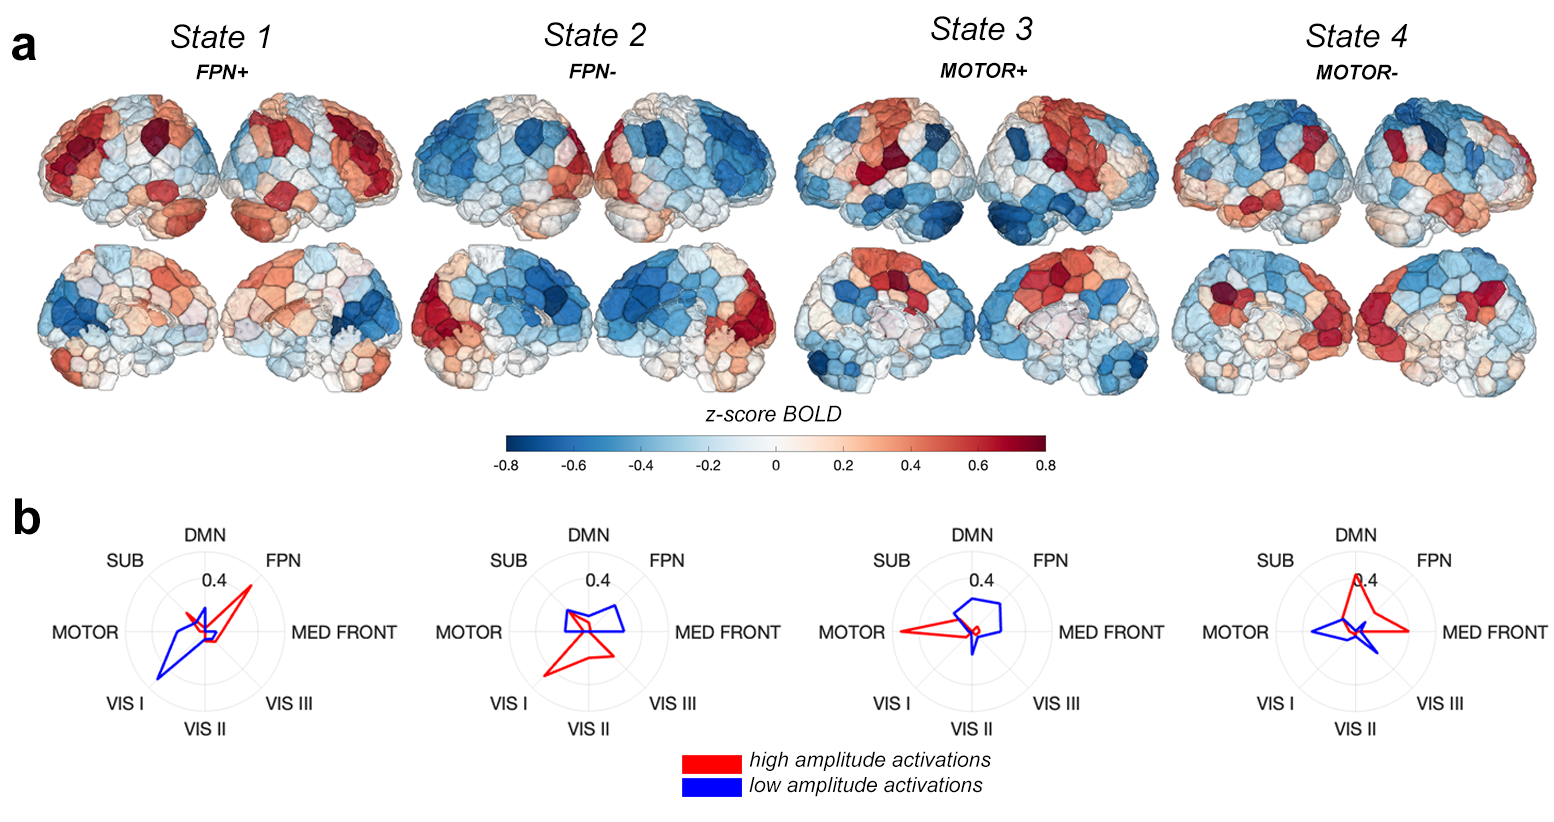
\includegraphics[width=1\textwidth]{chapter2/Figure2ab.png}
    \caption[]{}
\end{figure}
\null
\vfill
\clearpage    
    \null
\vfill
\begin{figure}[h!]
		\ContinuedFloat
		\captionsetup{labelformat=adja-page}
    \centering
    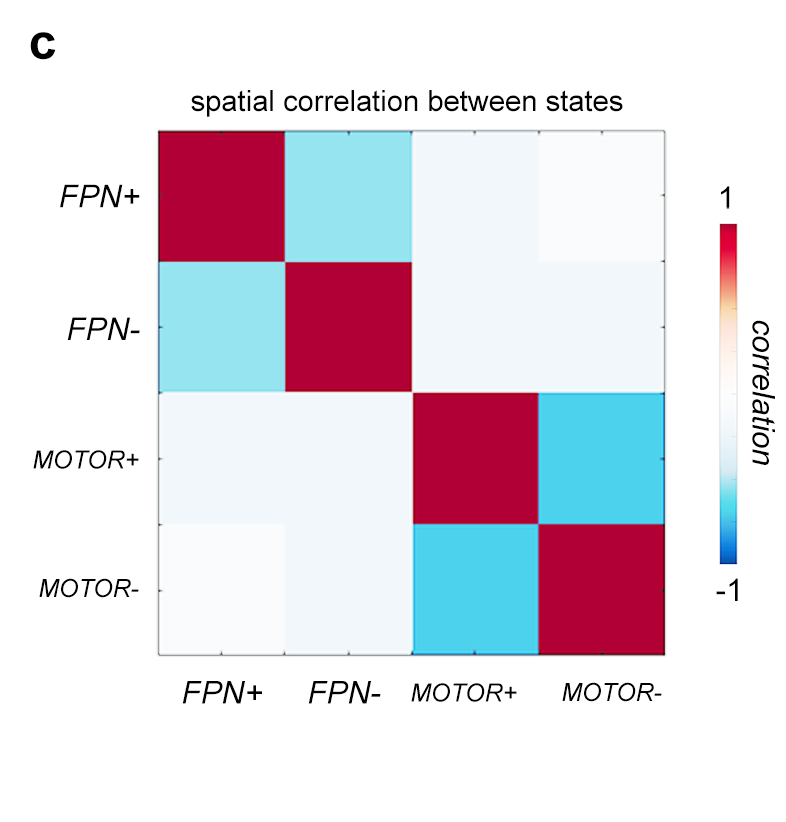
\includegraphics[width=1\textwidth]{chapter2/Figure2c.png}
    \caption[]{}
\end{figure}
\null
\vfill

    \subsection*{Stroke-control differences in brain state dynamics}

    Fractional occupancy (FO), dwell time (DT) and appearance rate (AR) of each state were calculated for each subject (Figure \ref{Figure2_1}a,b). Because the control subjects were younger on average than the stroke subjects, we assessed the correlation between age and brain state dynamic parameters in both groups (Figure \ref{2_SupplementaryFigure9}) and determined that there was no relationship between age and any parameter for any state for stroke or control subjects. The average FO, DT, and AR across all available time points (1 week, 2 weeks, 1 month, 3 months and 6 months) for each of the four states were compared between stroke and control subjects via unpaired two-tail t-tests (Figure \ref{Figure2_3}, see Figure \ref{2_SupplementaryFigure8} for full session-specific results for each state, and see Figure  \ref{2_SupplementaryFigure10} for the general pattern of brain dynamics observed in stroke and control subjects). Significantly lower fractional occupancy (FO) of $FPN^+$ in stroke subjects was observed at every session from 1 week to 6 months post-stroke (session 1 t-statistic: -2.18, 95$\%$ CI = [-0.0587,-0.0019], session 2 t-statistic: -3.36, 95$\%$ CI = [-0.0458,-0.014], session 3 t-statistic: -2.24, 95$\%$ CI = [-0.0435, -0.0023], session 4 t-statistic: -2.14, 95$\%$ CI = [-0.0516,-0.0016], session 5 t-statistic: -2.0725, 95$\%$ CI = [-0.0553,-0.0007], p(FDR) for all 5 tests $<$ 0.05) (Figure \ref{Figure2_3}a). Differences in dwell times (DT) of $FPN^+$ observed only in the chronic stage of stroke (6 months post-stroke) (p(FDR) = 0.0315, corrected over 5 tests) (Figure \ref{Figure2_3}c). Stroke subjects had significantly lower time-averaged FO in $FPN^+$ compared to control subjects (t-statistic: -3.7334,  95$\%$ CI = [-0.0425,-0.0127], p(FDR) = 0.0021), which was possibly driven more by the significantly lower dwell times in $FPN^+$ observed in stroke subjects (p(FDR) = 0.0105) (Figure \ref{Figure2_3}b,d). The frontoparietal network used in this atlas contains nodes in the dorsolateral prefrontal cortex, posterior parietal cortex, as well as nodes in the posterior inferior temporal lobe and the inferior cerebellum.  No differences in appearance rate of $FPN^+$ were observed over the sessions (Figure 3e, f).

\null
\vfill
\clearpage
\null
\vfill
\begin{figure}[h!]
    \centering       \caption{Group differences in brain state dynamics for $FPN^+$. }
  \caption*{ \textbf{a, c, e.} Stroke-control differences in session-specific fractional occupancy (FO), dwell time (DT), and appearance rate (AR) in $FPN^+$ over the post-stroke recovery period. \textbf{c, d, f} Stroke-control differences in average FO, DT, and AR (averaged over each subject's 2-5 longitudinal sessions). Hashtags ($\#$) represent p-values $<$ 0.05 after multiple comparisons correction within each parameter (i.e. FO, DT, AR), single asterisks ($*$) represent significant uncorrected p-values $<$ 0.05. Dwell time shown in units of TRs. n=24 biologically independent control subjects at each time point; n=23, 23, 22, 21, 20 biologically independent stroke subjects for time point 1, 2, 3, 4, and 5 respectively. On each box, the central mark indicates the median, and the bottom and top edges of the box indicate the 25th and 75th percentiles, respectively.}
      \label{Figure2_3}
\end{figure}

\null
\vfill
\clearpage
\null
\vfill
\begin{figure}[h!]
		\ContinuedFloat
		\captionsetup{labelformat=adja-page}
    \centering
    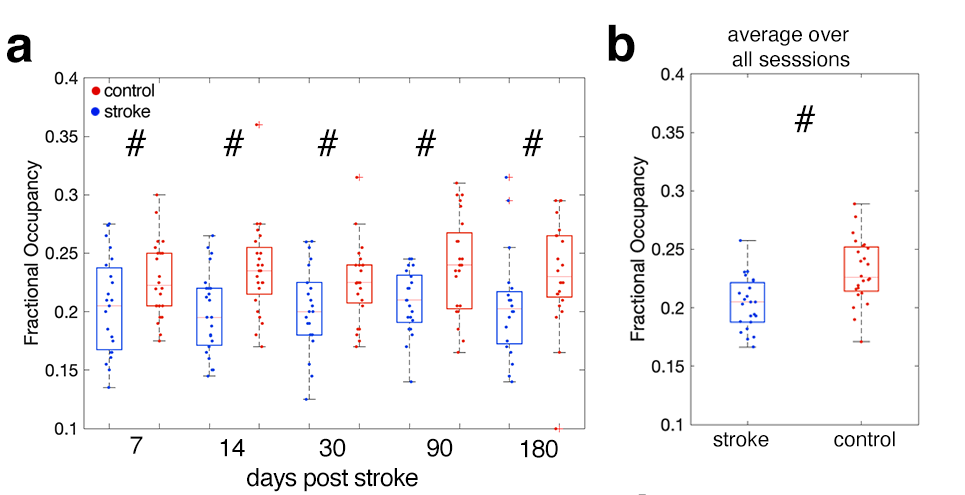
\includegraphics[width=1\textwidth]{chapter2/Figure3ab.png}
    \caption[]{}
\end{figure}
\null
\vfill
\clearpage    
    \null
\vfill
\begin{figure}[h!]
		\ContinuedFloat
		\captionsetup{labelformat=adja-page}
    \centering
    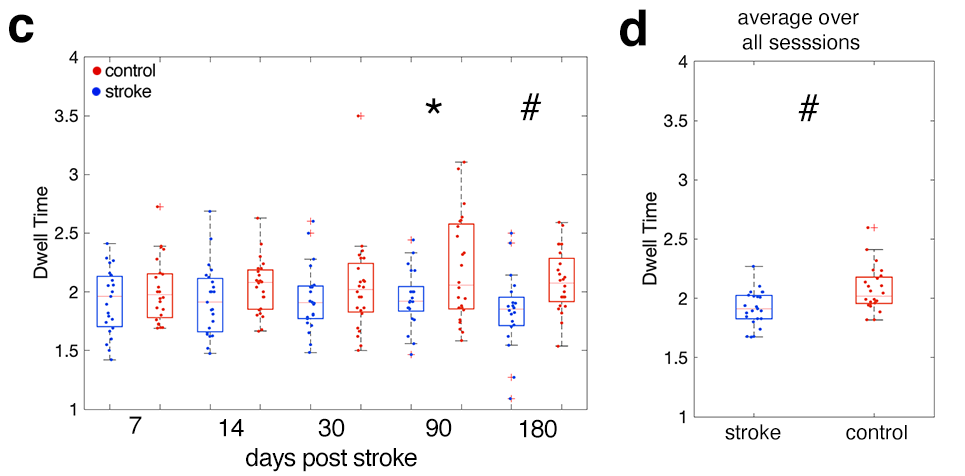
\includegraphics[width=1\textwidth]{chapter2/Figure3cd.png}
    \caption[]{}
\end{figure}
\null
\vfill
 \clearpage    
    \null
\vfill
\begin{figure}[h!]
		\ContinuedFloat
		\captionsetup{labelformat=adja-page}
    \centering
    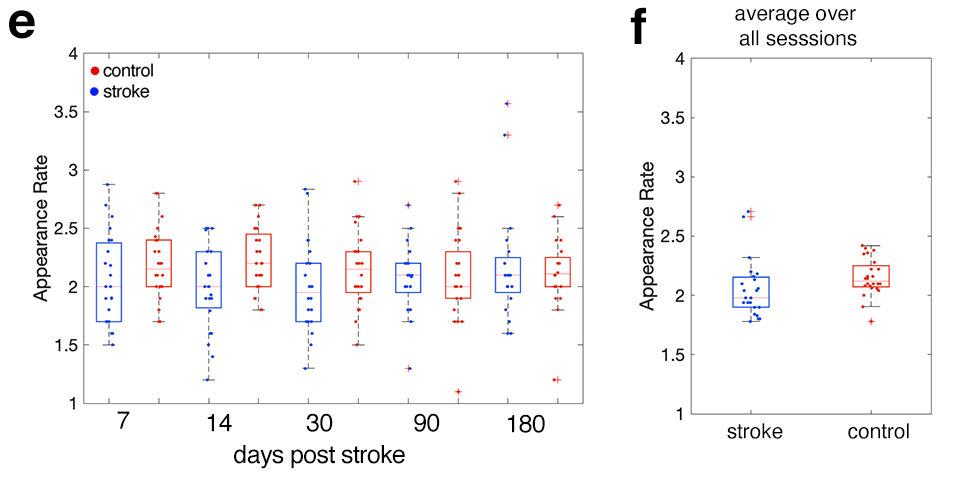
\includegraphics[width=1\textwidth]{chapter2/Figure3ef.png}
    \caption[]{}
\end{figure}
\null
\vfill
 \clearpage    
 
 
\clearpage

    Stroke subjects had significantly reduced transition probabilities from \begin{Large}$FPN^+$\end{Large} and \begin{Large}$MOTOR^-$\end{Large} into \begin{Large}$FPN^+$\end{Large} (p(FDR) = 0.023 and 0.020,  respectively) (Figure \ref{Figure2_4}a, b). The lower persistence probability in stroke for \begin{Large}$FPN^+$\end{Large} seems to be driven by chronic-stage differences; in the session-specific analysis, individuals with stroke have significantly lower persistence probability for \begin{Large}$FPN^+$\end{Large} at the 6-month time point (p(FDR) = 0.030) and there is a trend for lower persistence probability at 3 months (Figure \ref{Figure2_4}c).
    

\null
\vfill
\clearpage
\null
\vfill
\begin{figure}[h!]
    \centering       \caption{Differences in transition probabilities between stroke and control groups. }
  \caption*{Transition probabilities include persistence probabilities, i.e. the probability that a state does not transition out of itself. \textbf{a.} Differences in average  transition and persistence probabilities (over time) between groups. \textbf{b.} Same data as panel A, visualized with arrows colored by t-statistic. Hashtag ($\#$) next to arrows represent a significant group difference that survives multiple comparisons correction within each time point. \textbf{c.} Differences in transition probabilities at each follow-up session. T-statistics (stroke-control) are displayed on the color map; hashtags ($\#$) represent p-values $<$ 0.05 after multiple comparisons correction, single asterisks ($*$) represent significant uncorrected p-values $<$ 0.05.  n=24 biologically independent control subjects at each time point; n=23, 23, 22, 21, 20 biologically independent stroke subjects for time point 1, 2, 3, 4, and 5 respectively. }
      \label{Figure2_4}
\end{figure}

\null
\vfill
\clearpage
\null
\vfill
\begin{figure}[h!]
		\ContinuedFloat
		\captionsetup{labelformat=adja-page}
    \centering
    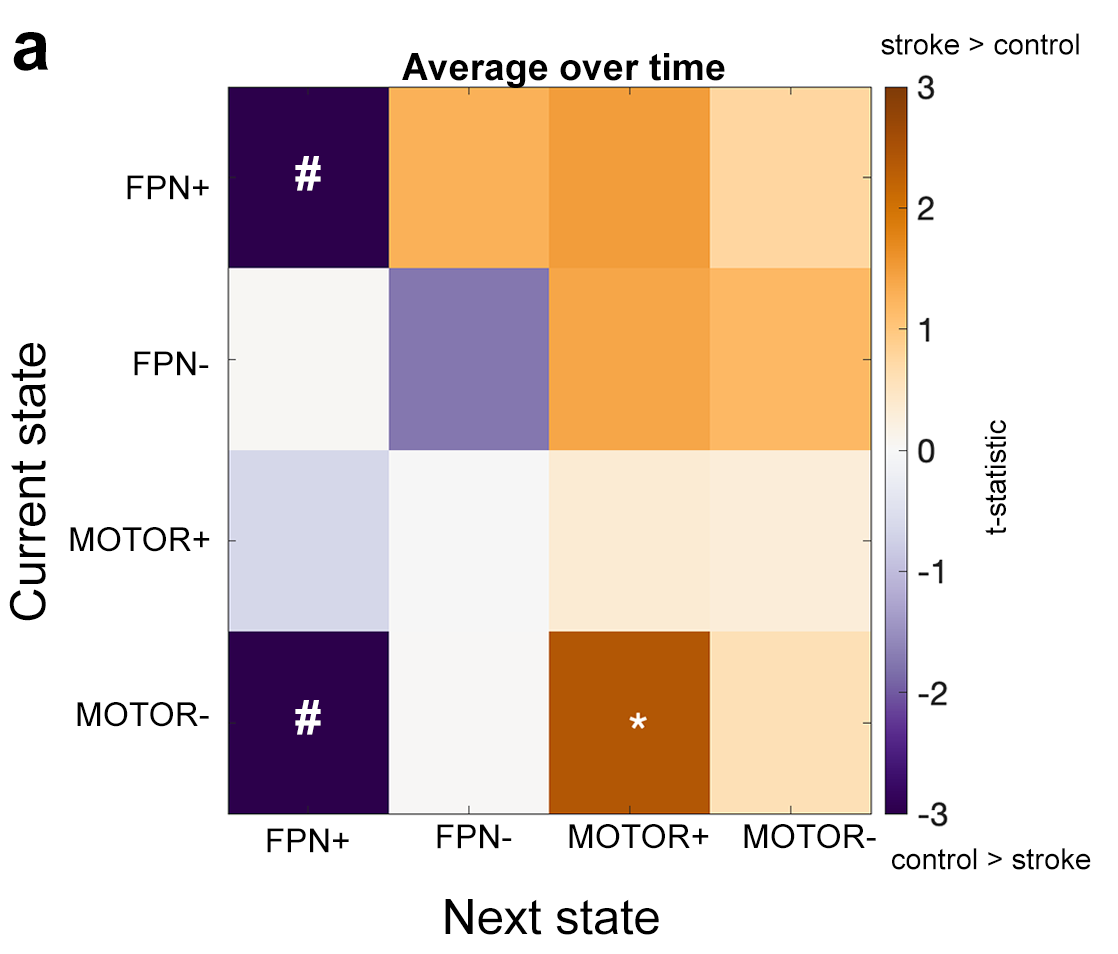
\includegraphics[width=1\textwidth]{chapter2/Figure4a.png}
    \caption[]{}
\end{figure}
\null
\vfill
\clearpage    
    \null
\vfill
\begin{figure}[h!]
		\ContinuedFloat
		\captionsetup{labelformat=adja-page}
    \centering
    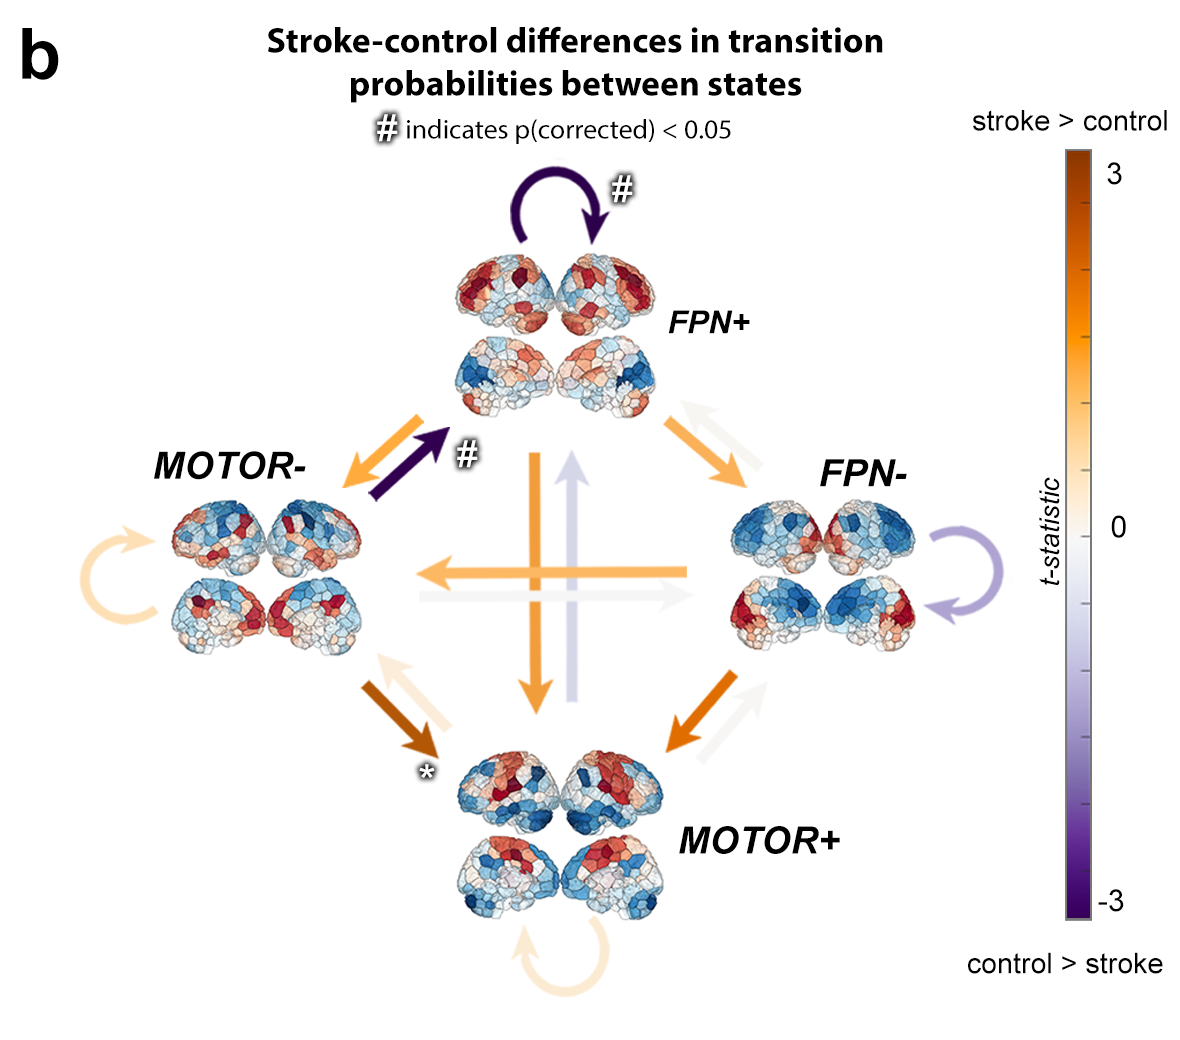
\includegraphics[width=1\textwidth]{chapter2/Figure4b.png}
    \caption[]{}
\end{figure}
\null
\vfill
\clearpage    
    \null
\vfill
\begin{figure}[h!]
		\ContinuedFloat
		\captionsetup{labelformat=adja-page}
    \centering
    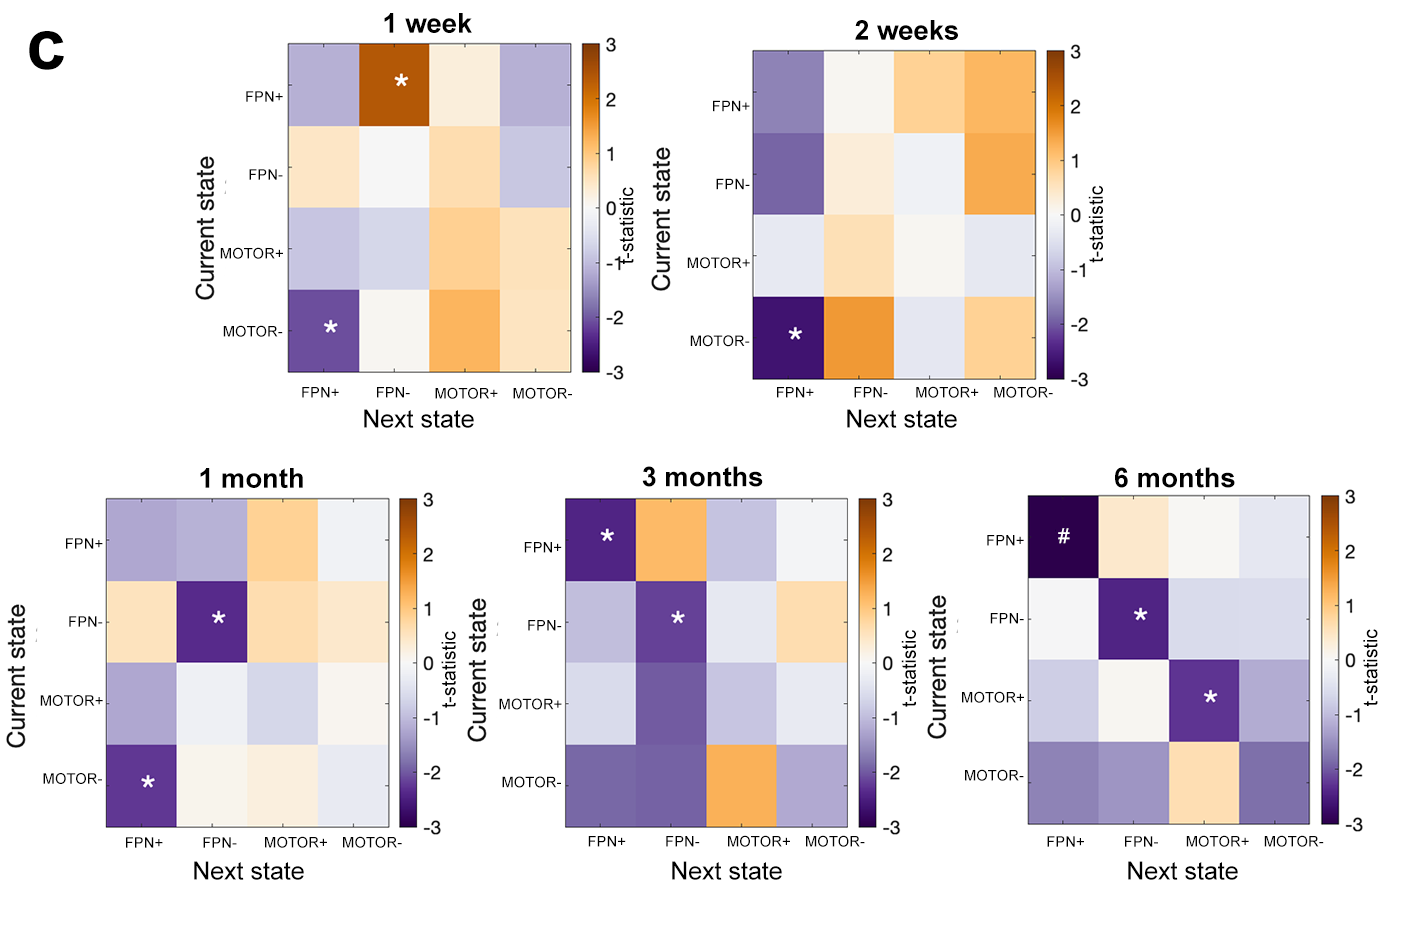
\includegraphics[width=1\textwidth]{chapter2/Figure4c.png}
    \caption[]{}
\end{figure}
\null
\vfill



    \subsection*{Frontoparietal activation relates to motor recovery in individuals with dominant-hand CST damage}
    
    We observed a significant interaction effect between changes in \begin{Large}$FPN^+$\end{Large} parameters and dominant-hand CST damage on changes in Fugl-Meyer scores (\begin{Large}$CST_D *\Delta FO^{FPN^+}_{chronic}$\end{Large}:  p(FDR) = 0.0091, \begin{Large}$CST_D *\Delta FO^{FPN^+}_{chronic}$\end{Large}: p(FDR) = 0.0090), as well as a significant association between changes in \begin{Large}$FPN^+$\end{Large} parameters and changes in Fugl-Meyer scores for subjects with dominant-hand CST damage (i.e., marginal effects) (\begin{Large}$\Delta DT^{FPN^+}_{chronic}$\end{Large}: p(FDR) = 0.0091,  \begin{Large}$\Delta FO^{FPN^+}_{chronic}$\end{Large}: p(FDR) = 0.0098), such that increases in (or smaller decreases in) dwell times in these subjects were associated with greater motor improvements (Figure 5). We confirmed the accuracy of our models by verifying that the residuals were normally distributed (Supplementary Figure 13). Some individuals with dominant-hand CST damage show decreases in $FPN^+$ recruitment over time, but smaller decreases in \begin{Large}$DT^{FPN^+}$\end{Large} and \begin{Large}$FO^{FPN^+}$\end{Large} are associated with better recovery. Including age and sex in the models does not alter the results (\begin{Large}$CST_D *\Delta FO^{FPN^+}_{chronic}$\end{Large}:  p(FDR) = 0.0166 , \begin{Large}$CST_D *\Delta FO^{FPN^+}_{chronic}$\end{Large}: p(FDR) = 0.0301, marginal \begin{Large}$\Delta FO^{FPN^+}_{chronic}$\end{Large}: p(FDR) = 0.016, \begin{Large}$\Delta DT^{FPN^+}_{chronic}$\end{Large}: p(FDR) = 0.016). The marginal effect for the dwell time analysis was replicated in k=5 (Figure \ref{2_SupplementaryFigure11}) but not the interaction effect, nor either effect for fractional occupancy. 
    
    Finally, we observe that there was a strong and significant correlation between baseline FM and \begin{Large}$\Delta DT^{FPN^+}_{chronic}$\end{Large} and \begin{Large}$\Delta FO^{FPN^+}_{chronic}$\end{Large} for subjects with dominant-hand CST damage (R = -0.83, p = 0.0054, R = -0.71 p = 0.033, respectively), see (Figure \ref{2_SupplementaryFigure14}a,b), such that subjects with more baseline impairment had the greatest increases in \begin{Large}$\Delta DT^{FPN^+}$\end{Large} and \begin{Large}$\Delta FO^{FPN^+}$\end{Large} from baseline to chronic time points. Therefore, we proceeded with creating the null model as described in the Methods section to verify that the observed relationships between \begin{Large}$\Delta FM$\end{Large} and \begin{Large}$\Delta DT/FO^{FPN^+}_{chronic}$\end{Large} were not a byproduct of the correlation with baseline $FM$. Indeed, the observed correlation between \begin{Large}$\Delta FM$\end{Large} and \begin{Large}$\Delta DT^{FPN^+}_{chronic}$\end{Large} is significantly greater than the null distribution of correlation between simulated proportional recovery and \begin{Large}$\Delta DT^{FPN^+}_{chronic}$\end{Large} (p = 0.0240) (Figure \ref{2_SupplementaryFigure14}c). However, the observed correlation between \begin{Large}$\Delta FM$\end{Large} and \begin{Large}$\Delta FO^{FPN^+}_{chronic}$\end{Large} is not significantly greater than what is observed in the null distribution (p = 0.50) (Figure \ref{2_SupplementaryFigure14}d). This suggests that the observed relationship between \begin{Large}$\Delta FM$\end{Large} and \begin{Large}$\Delta DT^{FPN^+}_{chronic}$\end{Large} in subjects with dominant hemisphere CST damage is not merely due to baseline correlations and proportional recovery, whereas that the relationship between \begin{Large}$\Delta FM$\end{Large} and \begin{Large}$\Delta FO^{FPN^+}_{chronic}$\end{Large} may be driven by the degree of impairment at baseline. 

\begin{figure}[htp]
 	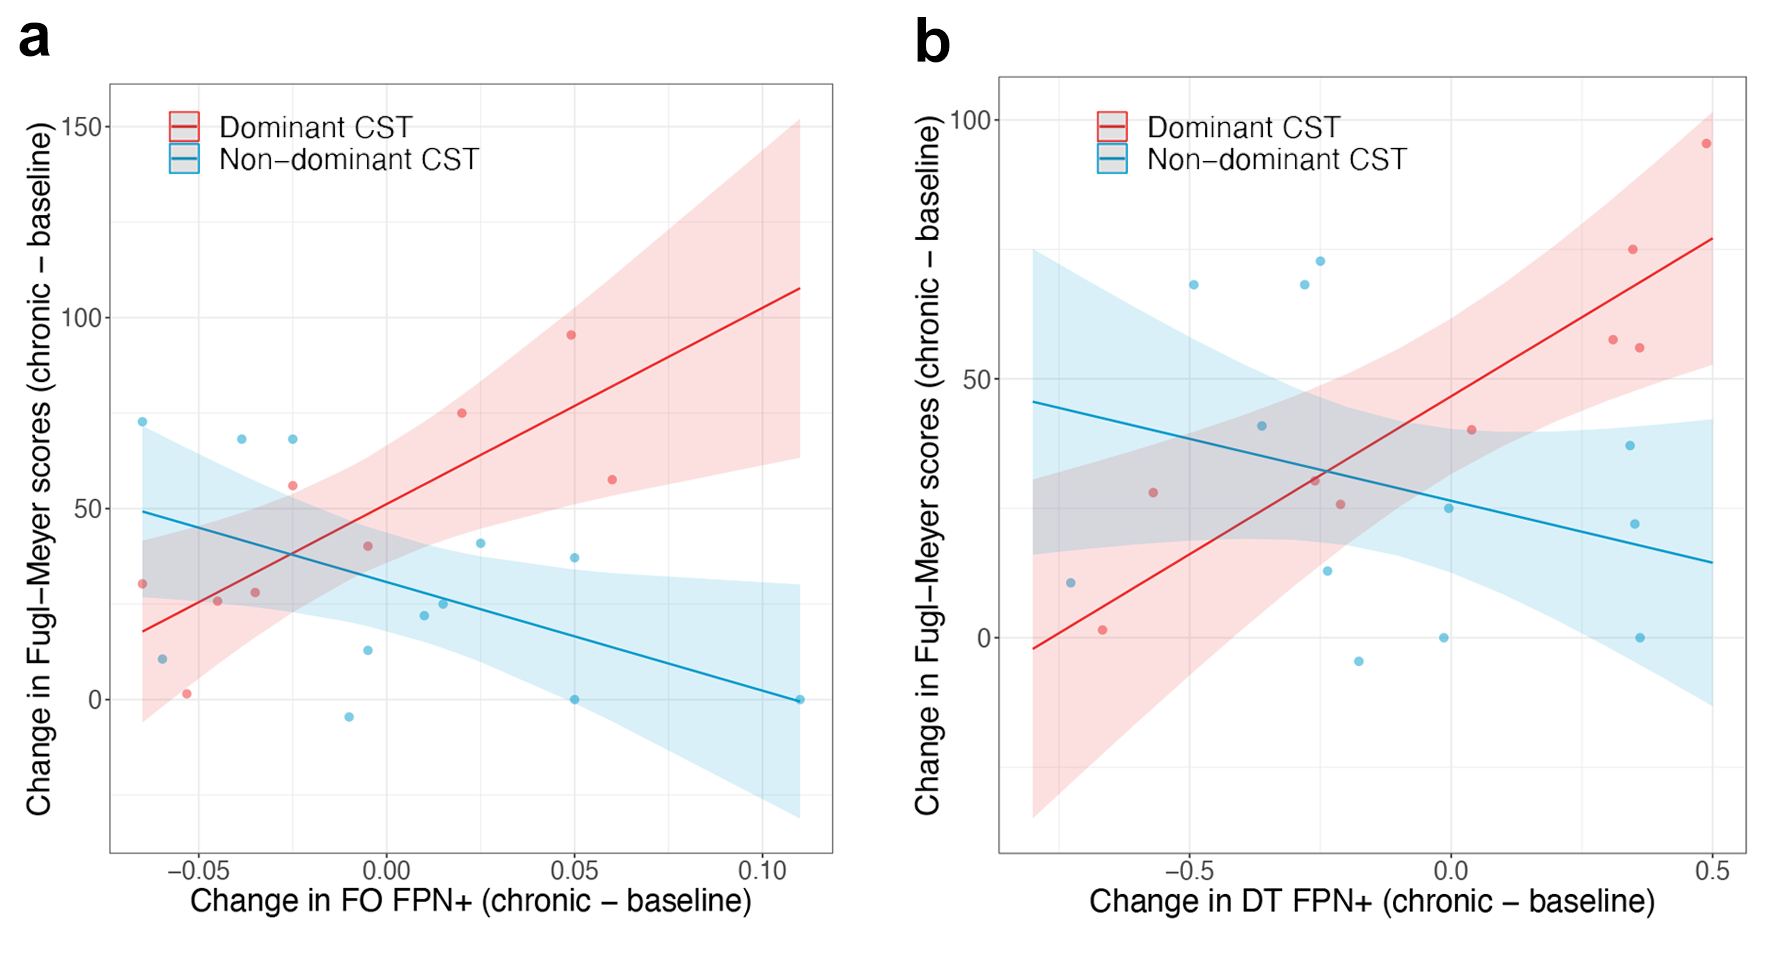
\includegraphics[width=1\linewidth]{chapter2/Figure5.png}
	\caption{Results from linear models with N=21 for each model. Colors indicate the marginal effects plots of change in state metrics within the regression model. Marginal effects plots of the change in Fugl-Meyer scores versus the change in fractional occupancy (FO) (\textbf{a}) and dwell time (DT) (\textbf{b}) of $FPN^+$ from baseline to chronic time points. Shaded bars indicate 95 percent confidence intervals. }
	\label{Figure2_5}
    \end{figure}
    

    \subsection*{Fractional occupancy differences are related to functional connectivity differences}
    Four network pairs had a high magnitude contra-activation (large amplitude activity in opposite directions) in the \begin{Large}$FPN^+$\end{Large} state: visual I (VIS I) and frontoparietal (FPN), subcortical/cerebellum (SUB) and visual I (VIS I), motor (MOTOR) and subcortical/cerebellum (SUB), and motor (MOTOR) and frontoparietal (FPN). Two pairs of networks had high magnitude co-activation (large amplitude activity in the same direction) in the \begin{Large}$FPN^+$\end{Large} state: SUB and FPN, and MOTOR and VIS I (Figure \ref{Figure2_6}a). For each individual, we correlated \begin{Large}$FO^{FPN^+}$\end{Large} with the FC between each pair of co-activated and contra-activated networks, expecting two trends. First, for the highly contra-activated network pairs, we expected a negative correlation between \begin{Large}$FO^{FPN^+}$\end{Large} and FC, as more time spent in \begin{Large}$FPN^+$\end{Large} would make the correlation between those networks more negative. Second, for the highly co-activated network pairs, we expected a positive correlation between \begin{Large}$FO^{FPN^+}$\end{Large} and FC as more time spent in this state would make the correlation between those networks more positive. We did indeed observe the expected relationships for all pairs of networks (Figure \ref{Figure2_6}b), where the strongest relationships between FC and \begin{Large}$FO$\end{Large} were observed for those network pairs that had the greatest recruitment in \begin{Large}$FPN^+$,\end{Large} as measured by cosine similarity with the \begin{Large}$FPN^+$\end{Large} centroid (VIS I and FPN). Further, we see that the correlation between \begin{Large}$FO^{FPN^+}$\end{Large} and FC is preserved across and within the groups and is not driven by across-group differences (Simpson's paradox).
    Finally, dynamic fluctuations in  \begin{Large}$FO^{FPN^+}$ \end{Large} track changes in dynamic FC within frontoparietal areas (Figure \ref{Figure2_6}c, d, e), where the average correlation across subjects between sliding-window FC and  \begin{Large}$FO^{FPN^+}$ \end{Large} is 0.29 (p = 0, assessed by permutation).

\null
\vfill
\clearpage
\null
\vfill
\begin{figure}[h!]
    \centering       \caption{Assessing the relationship between fractional occupancy of \begin{Large} $FPN^+$ \end{Large} and functional connectivity within the frontoparietal network.}
  \caption*{\textbf{a.} Pairs of highly activated Yeo networks in  \begin{Large}$FPN^+$ \end{Large}. \textbf{b.} Functional connectivity (FC) between co-activated and contra-activated networks in  \begin{Large}$FPN^+$ \end{Large} is related to fractional occupancy (FO) of   \begin{Large}$FPN^+$ \end{Large} ( \begin{Large}$FO^{FPN^+}$ \end{Large}) in both stroke and control subjects. Specifically, fewer TRs in a state with strongly contra-activated/co-activated networks results in smaller magnitude FC between those networks. \textbf{c.} Areas with high activation in the  \begin{Large}$FPN^+$ \end{Large} centroid. \textbf{d.} Dynamic, sliding-window fluctuations in  \begin{Large}$FO^{FPN^+}$ \end{Large} correlate with dynamic FC between regions highly active in the FPN (areas in \textbf{c}). \textbf{e} Subject-average correlation between dynamic, sliding window  \begin{Large}$FO^{FPN^+}$ \end{Large} and FC of regions highly active in  \begin{Large}$FPN^+$ \end{Large} (black line) and a null distribution of 100 subject-average correlations between dynamic, sliding-window  \begin{Large}$FO^{FPN^+}$ \end{Large} and FC in a set of randomly selected regions (blue histogram).}
      \label{Figure2_6}
\end{figure}

\null
\vfill
\clearpage
\null
\vfill
\begin{figure}[h!]
		\ContinuedFloat
		\captionsetup{labelformat=adja-page}
    \centering
    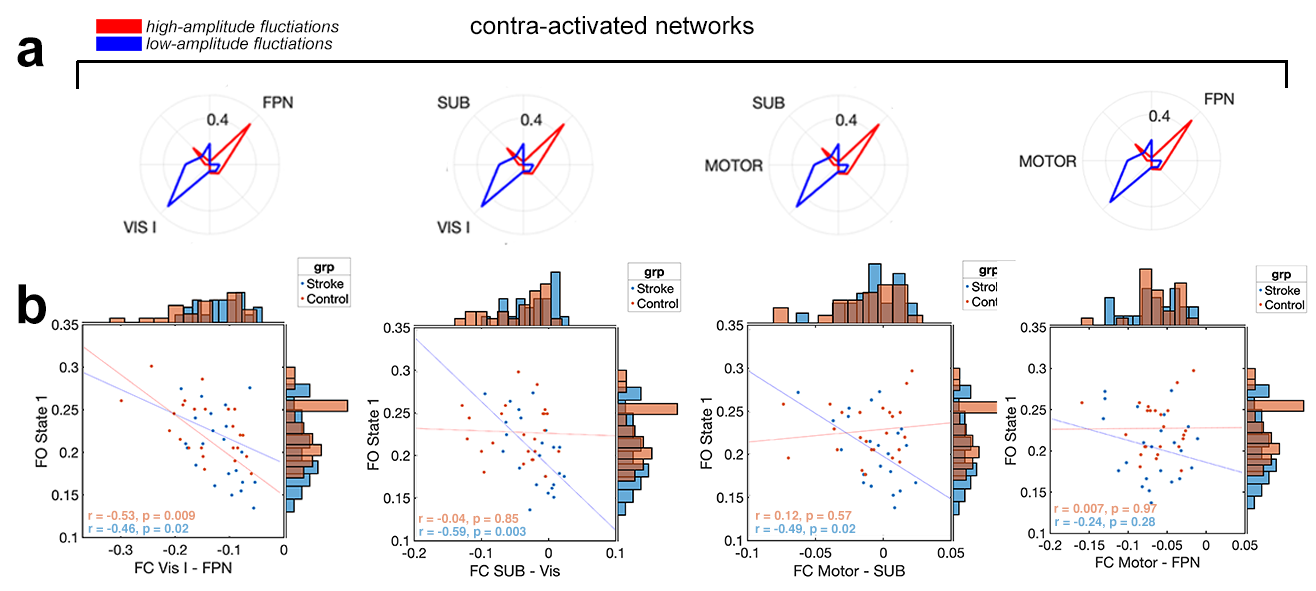
\includegraphics[width=1\textwidth]{chapter2/Figure6ab1.png}
    \caption[]{}
\end{figure}
\null
\vfill
\clearpage    
    \null
\vfill
\begin{figure}[h!]
		\ContinuedFloat
		\captionsetup{labelformat=adja-page}
    \centering
    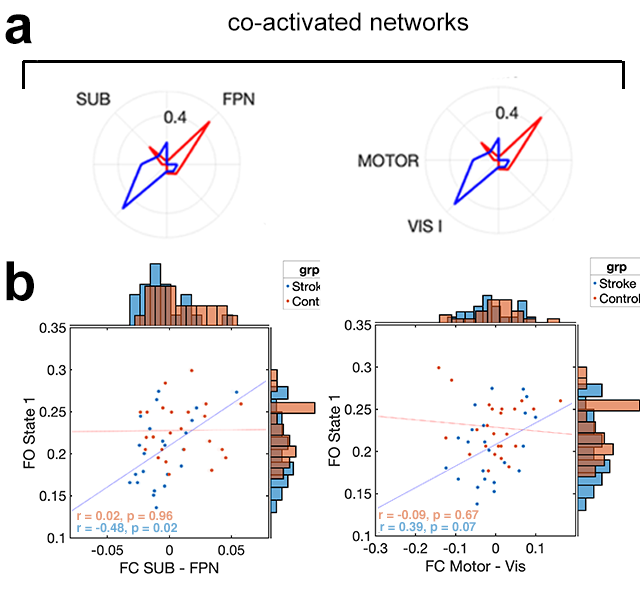
\includegraphics[width=1\textwidth]{chapter2/Figure6ab2.png}
    \caption[]{}
\end{figure}
\null
\vfill
\clearpage    
    \null
\vfill
\begin{figure}[h!]
		\ContinuedFloat
		\captionsetup{labelformat=adja-page}
    \centering
    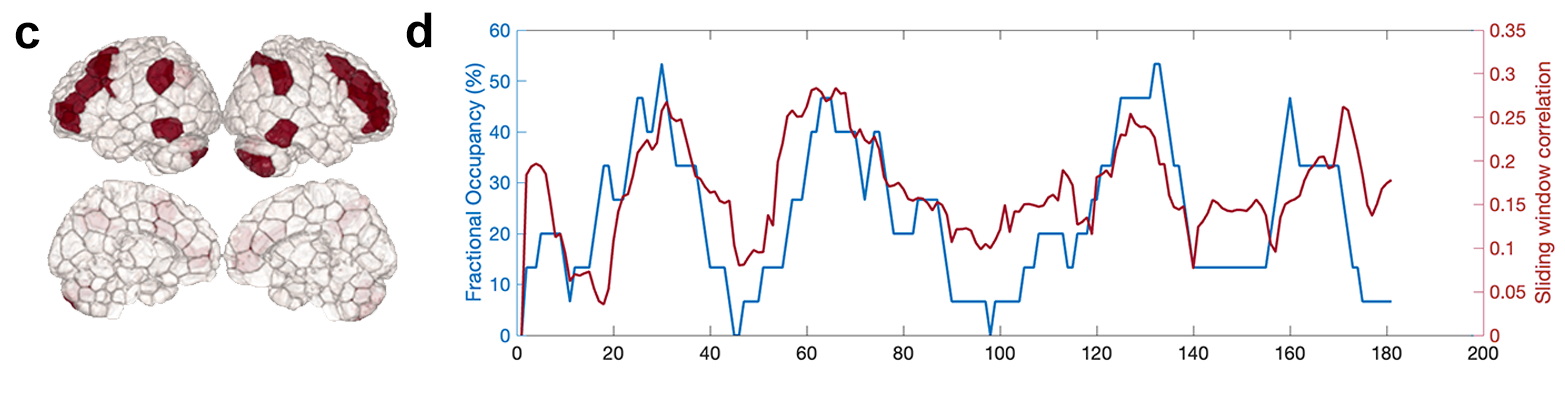
\includegraphics[width=1\textwidth]{chapter2/Figure6cd.png}
    \caption[]{}
\end{figure}
\null
\vfill
\clearpage    
    \null
\vfill
\begin{figure}[h!]
		\ContinuedFloat
		\captionsetup{labelformat=adja-page}
    \centering
    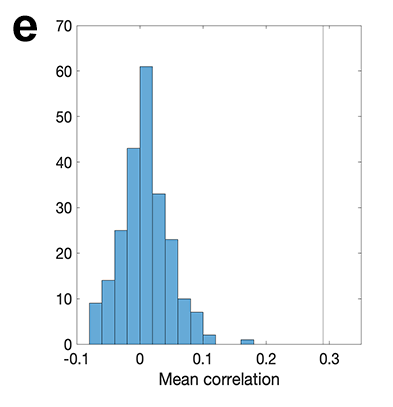
\includegraphics[width=1\textwidth]{chapter2/Figure6e.png}
    \caption[]{}
\end{figure}
\null
\vfill
\clearpage    
    \null
\vfill

\section{Discussion}
Large-scale brain activity patterns, or states, can be thought of as group-level temporal building blocks of canonical functional connectivity, reflecting sequences of activity that lie 'under the hood' of functional connectivity. Mapping the dynamics of these states offers a fine-grained view into shifts in the temporal sequences of neural activity after stroke that has not yet been explored. In the present study, we provide evidence that spatiotemporal brain dynamics, particularly in a state characterized by high-amplitude frontoparietal activity, are altered after pontine stroke for at least up to 6 months post-infarction. We further demonstrate that increased dwell time in this frontoparietal state is meaningfully related to better improvements in motor function for individuals with dominant-hand CST damage. Finally, we show a direct relationship between time spent in brain states and functional connectivity both in controls as well as individuals with stroke.

    %\subsection{Persistent reduced activation of the frontoparietal network in stroke}
    We observed that stroke subjects spent less time in a brain state characterized by high amplitude frontoparietal network activation, particularly in the sub-acute to chronic stages of stroke (3 and 6 months post-stroke). The frontoparietal network, containing nodes in the frontal cortex like the dorsal premotor cortex and in the parietal cortex like the posterior parietal cortex and intraparietal sulcus, is thought to act as a top-down influence on primary motor networks to control motor output (\cite{Marek2018-ql}). Communication between nodes in the frontoparietal network is known to be important for computations involved in goal-directed movement, such as motor imagery (\cite{Oostra2016-ki}), prospective action judgements (\cite{Geers2021-pz}), and generating appropriate hand positions to interact with objects (\cite{Borra2017-aj}). Evidence of reduced FC within the frontoparietal network has been observed in subcortical stroke subjects (\cite{Wang2014-vi}), as has reduced effective connectivity of the frontoparietal network on the motor network (\cite{Inman2012-tq}). Our study extends this current knowledge by demonstrating that the influence of the frontoparietal network in stroke subjects may be weakened, with reduced time spent in states with high amplitude frontoparietal activity.
    
    We did not observe changes in the fractional occupancy, dwell time, or appearance rate of the  \begin{Large}$MOTOR^+$ \end{Large} or  \begin{Large}$MOTOR^-$ \end{Large} states in stroke subjects, as one may anticipate after damage to the corticospinal tract. Instead, we observed changes in the transition probabilities between  \begin{Large}$MOTOR^-$ \end{Large} and  \begin{Large}$FPN^+$ \end{Large}, and  \begin{Large}$MOTOR^-$ \end{Large} and  \begin{Large}$MOTOR^+$. \end{Large} These may be more subtle impacts of corticospinal tract disruption that change the sequence of states visited at rest. A lack of differences in the  \begin{Large}$MOTOR$ \end{Large} states could also arise due to the fact that the method cannot detect differences in the magnitude of activations. A critical step in the method involves normalizing each region’s brain activity before clustering. This step would theoretically remove stroke-related differences in the magnitude of activation of motor areas that one may expect after CST damage. As the focus of our paper was to explore stroke-related changes in the temporal patterns of brain activity, we did not explore this possibility, but future work should examine changes in both the magnitude and temporal properties of these states after stroke. 
    
    
    %\subsection{Longer frontoparietal dwell time is associated with better chronic motor recovery in individuals with dominant CST damage}
    Recent work has shown that individuals with CST damage (measured using motor-evoked potentials) have greater resting-state functional connectivity in the frontoparietal network compared to individuals without CST damage (\cite{Hordacre2021-ct}). We observed that individuals with dominant-hand CST damage had a positive relationship between changes in motor recovery and changes in dwell times in the  \begin{Large}$FPN^+$ \end{Large} state from 1 week to the chronic time period post stroke. Increased time spent in the frontoparietal network in subjects with dominant hemisphere CST damage may be a form of compensation related to structural reserve capacity, a concept believed to reflect increased neural substrate that is neuroprotective against stroke and can modify outcomes (\cite{Rosenich2020-ef}). This result, from an exploratory analysis, suggests that frontoparietal activation may be an adaptive strategy to support motor recovery which may be more relevant for subjects with dominant hemisphere CST damage. This hypothesis requires formal examination in future research.
    
    %\subsection{Relationship of brain state dynamics and FC}
    Finally, we showed that across controls and individuals with stroke, FO of the \begin{Large}$FPN^+$\end{Large} state and FC between networks that dominate that state were related. For example, FC between pairs of networks that were co-activated in the\begin{Large} $FPN^+$\end{Large} state were positively correlated with FO and FC between pairs of networks that were contra-activated in the \begin{Large}$FPN^+$\end{Large} state were negatively correlated with FO. Less negative FC between the visual and FPN network was related to less time spent in \begin{Large}$FPN^+$\end{Large}, a state in which the two networks had large magnitude activations in opposite directions. Our findings suggest that time spent in certain brain states may underlie between-group FC differences; a finding which we also replicated with dynamic, sliding window analysis. Knowing how stroke and recovery from stroke is related to time spent in these states may be helpful in designing non-invasive stimulation strategies that are based on direct co-activation/conta-activation of certain regions or networks, not on indirect modulation of FC between pairs of regions/networks.  

    %\subsection{Clinical relevance}
    Consideration of state metrics like dwell times, fractional occupancy, appearance rate, and transition probability has the potential to be of great clinical relevance. Stimulation therapies like transcranial magnetic stimulation (TMS) activate or inhibit specific brain areas, often in an attempt to modulate networks whose connectivity has been associated with better recovery (\cite{Fisicaro2019-ly, Grefkes2010-jg, Fox2012-xz}). These stimulation methods may improve outcomes for those with stroke by permitting the development personalized treatment protocols. Recent TMS modelling work has shown that the effect of regional stimulation on FC depends on the brain state at the time of stimulation (\cite{Silvanto2008-um, Edwards2020-mr, Bergmann2018-re}). Determining subject-specific metrics of recurring patterns of brain activity may prove to have clinical benefit in the timing and spatial targets of stimulation treatments (\cite{Scangos2021-vy}).
    
    Furthermore, the discovery of the effect of the dominant hemisphere in this paper may aid in refining how treatments are individually tailored. In a recent paper, \cite{Hordacre2021-iu} propose a personalized model and suggest targeting alternative brain networks with tDCS. Based on this paper's findings, we conjecture that this form of stimulation may only be appropriate in those with damage to the dominant hemisphere CST. Additionally, the direction of neural activity changes underlying FC differences across pathological groups compared to control populations has not yet been fully quantified. We showed that analysing FC differences in the context of metrics of brain dynamics provides a more complete picture as to what activation patterns are driving observed differences. If the goal of stimulation therapies is to recapitulate functional network connectivity associated with better outcomes, then understanding how the activations within those networks give rise to connectivity differences may produce more effective targeting strategies.
    
   % \subsection{Limitations}
    There are several limitations to the study. First, the use of 4 clusters was chosen heuristically, and it is possible that more or fewer brain states exist in the stroke population. Second, k-means-based clustering of the time series does preserve the temporal resolution of brain states (as opposed to static or even dynamic functional connectivity), but with a few caveats. The true activation for a subject at a given time point is most similar to, but not identical to, the discrete cluster centroids described in this paper. There is significant variability in individual activation patterns which may be obscured by concatenating all subjects together and assigning each TR to a single, group-level cluster (\cite{Betzel2021-ve}). However, the goal of this study is to derive a meaningful group-level characterization of activity patterns after pontine stroke that may relate to motor recovery. Future work should address extending clustering results to individual subjects in order to support tailored treatments. Additionally, our fMRI sampling rate was 3 seconds which is too slow to capture faster, possibly relevant, brain dynamics  (\cite{Kobeleva2021-nv, Baker2014-zt}). Third, the frontoparietal network tends to be lateralized in motor-related activation; however, the clustering approach here uncovered a state with bilateral frontoparietal network activation. Therefore, determining whether contralesional or ipsilesional frontoparietal areas are more involved in recovery in subjects with dominant CST damage was not possible in this analysis. Fourth, the small sample size of subjects with dominant-hand CST damage limits confidence in the findings. Further analyses should attempt to replicate these findings with larger samples of subjects, including left-handed subjects with right hemisphere lesions. Additionally, CST integrity was assessed with the Dice coefficient and a population atlas which may not be accurate for all subject's neuroanatomy. Finally, most of the individuals with dominant-hand CST damage in the model had left-hemisphere lesions, so we cannot fully rule out whether the changes are associated with the left hemisphere or the dominant hemisphere specifically. Similarly, this method is limited in its ability to distinguish the separate contribution of the ipsilateral and contralateral sensorimotor areas, which are known to be differentially activated after stroke (\cite{Zemke2003-vs}), as it seeks to determine recurring states present in healthy controls and stroke subjects. As a result, we expect that our results reflect adaptations/disruptions to “canonical” brain activation states present across stroke and control populations (and may change after stroke in the proportion or frequency with which they are expressed). Further work that investigates more states, possibly states specific to the post-CST stroke brain, may elucidate the role of contralesional hemisphere activation, but that is beyond the scope of this study. 
    

\section{Conclusions}
    This work suggests that the temporal composition of brain activity is altered for up to 6 months after pontine stroke, with reduced time spent in a frontoparietal brain state in stroke subjects relative to control subjects. When the dominant-hand corticospinal tract is compromised, resting-state configurations may shift to include increased activation of alternative network configurations, like frontoparietal regions, to promote compensatory neural pathways that support recovery of motor function when traditional motor circuits of the dominant-hemisphere corticospinal tract are compromised. Determining subject- and  lesion-specific patterns of brain activity highly associated with recovery may help improve the design of clinical rehabilitation strategies, including non-invasive brain stimulation.


\label{chap:3}
\chapter{Systematic comparison of imaging biomarkers of chronic stroke motor outcome in the ENIGMA Stroke Recovery Working Group dataset}
\section{Introduction}
Stroke is a leading cause of long-term disability worldwide (\cite{Katan2018-qn}). Motor impairments are the most common deficit after stroke, and up to 50 percent of stroke survivors will have lasting hemiparesis (\cite{Kelly-Hayes2003-sp}). Providing accurate predictions of long-term motor outcomes is an ongoing goal of stroke research, as predictions based on acute clinical information can inform individualized rehabilitation strategies and can guide patient selection in clinical trials (\cite{Bonkhoff2022-op, Boyd2017-gs}). Biomarkers derived from routinely-collected structural neuroimaging data that reflect lesion location with respect to critical white matter tracts have been related to motor outcomes (\cite{Tozlu2020-qa, Kuceyeski2016-vj, Griffis2019-cy, Salvalaggio2020-pe, Bowren2022-rs}). However, there is no consensus on how to optimally model lesion-induced disruption of structural connections to produce generalizable predictions of chronic motor deficits. 

The most well-studied biomarker is the corticospinal tract (CST) lesion load, or the proportion of voxels in the ipsilesional corticospinal tract (typically originating from primary motor cortex, M1) that intersect with the lesion (\cite{Zhu2010-qh, Feng2015-du, Findlater2019-je, Lam2018-xh, Pineiro2000-dv}). M1-CST lesion load has been related to motor deficits in the acute and chronic phase of stroke (\cite{Boyd2017-gs, Kim2017-xe}), but M1-CST damage in itself is unlikely to capture enough variance in lesion data to explain motor deficits in patients with a wide range of lesion topographies (\cite{Park2016-te,Findlater2019-je}). Including damage to higher order motor areas explains more variance in post-stroke motor outcomes than damage to M1 alone (\cite{Ito2022-em,  Rondina2016-ds, Rondina2017-ij, Schulz2012-yy, Park2016-te}). For instance, \cite{Ito2022-em} use the sensorimotor tract template atlas to calculate lesion load (SMATT-LL) to several tracts originating from primary motor, premotor, somatosensory, and supplementary motor regions, and find that post-stroke motor outcomes are explained best by damage to fibers originating from M1 and from ventral premotor cortex. 

These somatomotor tracts were selected a priori on the basis of their known theoretical involvement in motor function. However, in the context of prediction, where we simply wish to exploit associations between lesion data and motor deficits with the goal of optimizing out-of-sample predictive accuracy, limiting input features to predefined structures in the motor system may limit model performance. Non-causal associations between damage and deficits exist in stroke because the distribution of lesions is influenced by vascular anatomy, and regions that are not related to a deficit may be consistently damaged alongside a critical region in a way that makes the two regions statistically indistinguishable (\cite{Mah2014-cb}). In other words, we may want to discover useful lesion-deficit associations in a data-driven way instead of assuming that theory-based structure-function relationships will have maximal predictive value (\cite{Bzdok2020-py, Bonkhoff2022-op}).

Lesion-behaviour mapping (LBM) is a technique used to discover neural correlates of a behavioural deficit that involves associating voxelwise lesion damage with the presence or degree of a deficit (\cite{Bates2003-eg,Karnath2020-cg}). Maps of association can be derived from multivariate models that relate deficits to patterns of damage across multiple voxels simultaneously (\cite{Ivanova2021-nh, Karnath2020-cg, Zhang2014-jd, Sperber2019-tu}). These multivariate models generate maps using one of two statistical frameworks: inference or prediction (\cite{Sperber2022-oj, Bzdok2020-py}). In an inference framework, these maps consist of voxels in which damage is significantly associated with a deficit. While inferential methods have been used successfully to evaluate hypotheses and generate explainable results, statistical significance does not necessarily imply good generalization performance (\cite{Bzdok2020-py}). On the other hand, in a prediction framework, lesion-behaviour maps are comprised of patterns of voxels in which damage is predictive of impairment in new subjects (\cite{Bowren2022-rs, Mah2014-cb,Rondina2017-ij, Sperber2020-kp}). Lesion-behaviour maps derived from a predictive framework may be more suitable as input features to predictive models, given that those maps to some degree already contain features in which damage predicts impairment in new subjects (\cite{Zhang2014-jd}). In light of the importance of the brain's structural networks in motor function, \cite{Bowren2022-rs} perform multivariate lesion-behaviour mapping to identify patterns of voxels in which damage predicts motor impairments. Then, they identify the structural connections that pass through the peak voxels identified with predictive LBM, thus placing the findings within the context of a broader disrupted structural network. Damage to those structural connections (lesion load on structural lesion network maps, sLNM-LL) as features in predictive models. These features are derived in a data-driven way from predictive multivariate lesion-behaviour mapping and have already shown promising predictive potential (\cite{Bowren2022-rs}), but have yet to be formally cross-validated in an independent dataset. 

Multivariate lesion-behaviour analyses (including \cite{Bowren2022-rs}) traditionally identify combinations of voxels in which damage is associated with a deficit. This high-dimensional, voxelwise lesion representation may hamper predictive models: when no patients have lesions in a given voxel, associations between damage and impairment cannot be detected (\cite{Kimberg2007-sk, Rorden2009-ae,Sperber2020-kp,Griffis2019-cy}). Instead of relating voxelwise lesion damage to deficits, one can first identify the white matter tracts that pass through the lesion using structural connectomes from healthy subjects as a reference, a technique known as structural disconnection-behaviour mapping (\cite{Kuceyeski2013-nk, Kuceyeski2016-vj, Salvalaggio2020-pe, Griffis2019-cy, Sperber2022-oj}). This is in effect a dimensionality reduction of voxelwise lesion data that can identify, for instance, damage to the same white matter tract by non-overlapping lesions. Projecting voxelwise lesion data into lower-dimensional structural disconnection space may be a biologically-relevant way to preserve variance in lesion-deficit relationships while improving statistical power. Using the Network Modification tool (\cite{Kuceyeski2013-nk}), the amount of lesion-induced structural disconnection for each gray matter region in the brain can be estimated. Similar to recent approaches in multivariate lesion behaviour mapping (\cite{Kasties2021-rm}), feature selection can be employed to identify subsets of regions that are relevant for predicting chronic motor scores in new subjects. Selecting features in a data-driven way and estimating the performance of resulting models often requires many subjects; with the rising availability of large stroke imaging databases (\cite{Liew2020-ps}), multivariate predictive models can be trained and evaluated in the same study.

In this paper, we compare the out-of-sample predictive performance of several lesion damage metrics using a large, diverse stroke imaging dataset (N = 789). First, we assess the predictive performance of theory-based biomarkers, including M1-CST-LL and SMATT-LL, that reflect damage to known somatomotor white matter tracts. We then evaluate the performance of data-driven biomarkers: sLNM-LL, which reflects damage to white matter tracts associated with peak voxels from multivariate predictive lesion-behaviour mapping, and ChaCo scores, which compress voxelwise data into regional structural disconnectivity measures. In this final model, we evaluate the use of feature selection to identify regions in which structural disconnectivity is predictive of chronic motor scores.

Our primary objective was to determine the relative performance of different biomarkers for predicting chronic motor scores, with the hypothesis that data-driven models would have superior prediction performance compared to theory-based biomarkers based in the motor system. As a secondary objective, we assessed whether predictive performance could be improved by incorporating demographic information and by combining predictions from several different biomarkers using ensemble models.

\section{Methods}

\subsection{Sample demographics}
A subset of cross‐sectional data from the Enhancing Neuroimaging Genomics through Meta Analysis (ENIGMA) Stroke Recovery Working Group database (available as of 10 Sept. 2021) was used in the study. Details of the ENIGMA Stroke Recovery procedures and methods are available in (\cite{Liew2020-ps}). The data originated from 22 research studies (sites) (Table \ref{table:Demographics}). Informed consent was obtained from all subjects, and data were collected in compliance with each institution’s local ethical review boards and in accordance with the Declaration of Helsinki.

ENIGMA Stroke Recovery participants with the following data were included: (1) high‐resolution (1‐mm isotropic) T1‐weighted brain MRI (T1w) acquired with a 3T MRI scanner; (2) information about time since stroke at time of imaging (3) age, (4), sex, and (5) measurem of motor function from one of the following assessments: Fugl Meyer Assessment of Upper Extremities (FMA‐UE), a performance-based measure of paretic upper extremity impairment (\cite{Gladstone2002-fw}); the Action Research Arm test (ARAT) which tests arm function through assessment of the timing and difficulty of motor task completion (\cite{Yozbatiran2008-xv}); the Barthel index, which measures the extent to which a person can function independently and has mobility in their activities of daily living (\cite{Sulter1999-rr}); National Institutes of Health Stroke Score (NIHSS), a broad measure of stroke severity that includes assessment of non-motor and motor functions (\cite{Lyden2017-za}). Motor scores were normalized to the range [0, 1] by dividing by the raw score by the maximum possible score on the assessment. For a majority of the chronic stroke subjects (76$\%$), motor deficits are normalized FMA‐UE scores, whereas  normalized FMA‐UE scores were available for only $12\%$ of the acute stroke subjects (for full breakdown of type of test used for each site in the dataset, see Supplementary Table \ref{motor_scores}). behavioural data were collected within approximately 72 hours of the MRI. Subjects were considered in the chronic phase of stroke if their time since stroke at the time of assessment was greater than 180 days, and considered in the acute phase if their time since stroke at the time of assessment was less than 180 days (\cite{Bernhardt2017-av}). Subjects with cortical and subcortical lesions were included in the study; lesions were not flipped (see Supplementary Figure \ref{lesiondist} for lesion distribution in MNI space). 

\newpage

\singlespacing
\begin{longtable}{c|c|c|c|c|c}
\caption[]{Demographic information of the acute subjects in the ENIGMA dataset, broken down by chronicity (acute/chronic) and by site within each chronicity group. Total sample size (N), number of females (F) and males (M), and information about age (years), normalized motor scores, time since stroke at the time of assessment (months), and lesion volume ($cm^3$). IQR, interquartile range\label{long}}\\

Site ID & Total N.  & Median age & Median   & Median   & Median  \\
& (F/M) & in years & motor score&  time since  & lesion vol,  \\
& &(IQR)  &  (IQR) & stroke (IQR)  & $cm^3$ (IQR)  \\
Acute & & & & & \\

\hline\hline
r005 & 1 (0/1) & 50.0 (0.0) & 0.29 (0.00) & 5.1 (0.0) & 1.7 (0.0) \\
r009 & 50 (13/37) & 70.0 (18.5) & 1.00 (0.05) & 0.2 (0.1) & 1.7 (7.0) \\
r025 & 9 (4/5) & 70.0 (19.0) & 1.00 (0.09) & 3.0 (1.0) & 0.5 (1.4) \\
r028 & 1 (0/1) & 63.0 (0.0) & 0.74 (0.00) & 5.5 (0.0) & 23.9 (0.0) \\
r031 & 36 (10/26) & 58.5 (13.2) & 0.52 (0.38) & 4.5 (1.7) & 10.8 (38.8)  \\
r038 & 72 (30/42) & 66.5 (21.2) & 0.78 (0.66) & 2.9 (2.3) & 11.5 (41.6)  \\
r040 & 57 (32/25) & 64.0 (22.0) & 0.40 (0.50) & 1.8 (1.5) & 14.7 (58.6)  \\
r047 & 2 (1/1) & 71.0 (2.0) & 0.59 (0.26) & 4.4 (0.2) & 23.8 (19.2)  \\
r049 & 21 (12/9) & 65.0 (16.0) & 0.95 (0.00) & 0.0 (0.0) & 1.3 (2.2)  \\
r050 & 14 (7/7) & 68.0 (16.8) & 0.92 (0.10) & 0.0 (0.0) & 0.3 (0.4)  \\
r053 & 52 (20/32) & 63.5 (20.5) & 0.92 (0.17) & 3.0 (3.0) & 13.5 (28.3)  \\
r054 & 12 (5/7) & 65.5 (11.8) & 0.67 (0.83) & 0.4 (0.2) & 4.1 (14.1)  \\
 & & & & & \\
Chronic & & & & & \\
\hline\hline
r001 & 39 (10/29) & 61.0 (17.0) & 0.65 (0.23) & 23.5 (40.0) & 6.3 (18.1)  \\
r002 & 12 (6/6) & 69.5 (11.5) & 0.50 (0.41) & 73.2 (51.9) & 28.2 (31.7)  \\
r003 & 15 (6/9) & 61.0 (16.5) & 0.24 (0.20) & 48.8 (67.6) & 20.3 (76.9)  \\
r004 & 19 (7/12) & 44.0 (14.5) & 0.17 (0.16) & 50.4 (81.9) & 36.9 (44.3)  \\
r005 & 27 (12/15) & 66.0 (16.5) & 0.79 (0.45) & 31.4 (27.8) & 1.6 (40.3)  \\
r009 & 60 (17/43) & 71.0 (7.2) & 0.96 (0.12) & 27.4 (9.3) & 1.4 (4.7) \\
r025 & 16 (3/13) & 64.5 (13.2) & 0.98 (0.58) & 14.2 (10.2) & 5.9 (14.3)  \\
r027 & 28 (8/20) & 57.0 (10.2) & 0.30 (0.16) & 19.3 (24.7) & 12.3 (62.1)  \\
r028 & 21 (6/15) & 63.0 (9.0) & 0.82 (0.24) & 26.5 (37.5) & 5.2 (41.3)  \\
r031 & 1 (0/1) & 52.0 (0.0) & 0.68 (0.00) & 6.1 (0.0) & 1.5 (0.0)  \\
r034 & 15 (6/9) & 58.4 (11.1) & 0.82 (0.20) & 61.3 (68.3) & 6.7 (35.0)  \\
r035 & 15 (6/9) & 64.0 (18.0) & 0.64 (0.52) & 33.5 (22.9) & 3.9 (31.6)  \\
r038 & 18 (7/11) & 67.0 (10.0) & 1.00 (0.12) & 15.1 (10.1) & 2.0 (1.6)  \\
r040 & 14 (7/7) & 63.5 (9.8) & 0.68 (0.47) & 14.1 (17.5) & 8.6 (82.7)  \\
r042 & 22 (11/11) & 48.5 (15.5) & 0.64 (0.19) & 29.6 (36.4) & 14.1 (49.5)  \\
r044 & 4 (0/4) & 68.0 (9.2) & 0.52 (0.25) & 43.7 (52.9) & 23.7 (67.0)  \\
r045 & 4 (1/3) & 62.0 (5.2) & 0.49 (0.24) & 96.1 (59.0) & 8.0 (6.7)  \\
r046 & 11 (3/8) & 62.0 (10.5) & 0.50 (0.29) & 86.3 (83.4) & 4.6 (19.8)  \\
r047 & 44 (14/30) & 65.5 (12.0) & 0.65 (0.44) & 38.1 (53.7) & 12.7 (41.3)  \\
r048 & 43 (16/27) & 68.0 (12.5) & 0.79 (0.44) & 46.2 (49.8) & 7.9 (43.4)  \\
 \caption[]{(continued)}\\

r052 & 32 (12/20) & 63.0 (13.5) & 0.41 (0.09) & 39.1 (42.2) & 7.0 (51.5)  \\

   & & & & & \\
 All  & & & & & \\
\hline\hline
& 789  & 64.0 & 0.7 & 12.2 & 6.5 \\
&(293/496) &(18.0) & (0.5) &(0.2) &  (32.5)  \\

\bottomrule
\end{longtable}

\doublespacing

\subsection{General overview}

We built several models to predict chronic motor scores from imaging data and minimal clinical information. Each model uses lesion-derived information as input to predict normalized motor scores in chronic stroke subjects. We compared several different features that reflect different aspects of lesion damage. These features include: lesion load to ipsilesional M1 (1 feature), lesion load of higher order motor tracts (6 features for ipsilesional tracts, 12 features in left and right hemisphere tracts together) structural lesion-behaviour mapping components (5 features based on \cite{Bowren2022-rs}), and measures of structural disconnection reflecting damage to gray matter regions across the entire brain (2 atlases assessed with 86 or 268 features; fewer with feature selection). We assessed whether data-driven feature selection improved performance for models using whole-brain measures of structural disconnection. Nested cross-validation was performed for all measures to train models and assess performance on unseen data.  Additionally, we evaluated whether including acute subjects in the training set (but not in the test set) improved prediction of chronic deficits, with the idea that the signal in the acute data would be useful in predicting deficits in the chronic phase. We also evaluated whether adding basic clinical information (age, sex, time since stroke) with ensemble models improved performance. Finally, we assessed whether using ensemble models to combine predictions from multiple different lesion damage metrics improved performance.

\subsubsection{Machine learning framework}
Models differed for each lesion biomarker based on the data; see below (3.3 Description of models and their inputs) for implementation details for each biomarker. In general, regression models were trained and evaluated using repeated 5-fold nested cross-validation loop.  In the outer loop, the data was split into 5 training and test partitions. Using only chronic data to train the models, there were approximately 370 subjects in the training set and 92 subjects in the test set. If acute data was used in training, it was added to the training partition, such that there were 696 subjects in the training set and 92 subjects in the test set. Training data was further partitioned into training and validation sets in the inner loop, and if hyperparameters were specified in the model, they were optimized in the inner loop. 

Out-of-sample performance was calculated as the average performance across 5 outer test folds. We obtained a distribution of out-of-sample performance by splitting the data into 5 train/test folds 100 times, shuffling the indices of the splits each time. 

\subsubsection{Model performance}
Model performance was assessed by comparing true normalized motor scores with predicted scores. Performance was calculated with Pearson's correlation coefficient and by the explained variance score, or $R^2$, which captures the percent of variation in motor scores explained by variation in the model predictors. Two performance metrics were used in order to compare results with prior literature, which uses both.

\subsection{Description of models and their inputs}
\subsubsection{Primary motor cortex CST lesion load (M1-CST-LL) models}

The lesion load of the corticospinal tract originating from the primary motor cortex (M1-CST-LL) has been associated with motor impairment (\cite{Stinear2017-eg}). Here, as in previous work, M1-CST-LL was calculated as the proportion of lesioned voxels intersecting with a binarized ipsilesional M1-CST template (\cite{Zhu2010-qh}). Specifically, lesion load was calculated in 1mm MNIv6 space as:
\begin{equation}
    \textit{Lesion load} = \frac{\textit{Number of lesioned voxels intersecting with  tract}}{\textit{Number of voxels in tract}}
\end{equation}
Left and right hemisphere M1-CST segmentations in MNI space were obtained from the high-resolution sensorimotor area tract template (SMATT) (\cite{Archer2018-ti}). M1-CST-LL had a heavy-tailed distribution (Supplementary Figure \ref{lesion_load_dist}A).
Linear regression was used to model the relationship between ipsilesional M1-CST-LL and chronic motor scores. The weights from best-performing model in the inner loop were used to predict motor scores for new subjects in the test folds. 

\subsubsection{Sensorimotor tract lesion load (SMATT-LL) models}
Sensorimotor tract segmentations were obtained from the sensorimotor area tract template (SMATT) (\cite{Archer2018-ti}), a set of 12 tracts derived from probabilistic tractography seeded in the left and right primary motor cortex (M1), dorsal and ventral premotor cortex (PMd and PMv, respectively), supplementary motor area (SMA), pre-supplementary motor area (pre-SMA), and primary somatosensory cortex (S1) of healthy controls (Figure \ref{smatt_and_chaco}A). Lesion load was calculated as above, for all 12 tracts, i.e., separately for left and right hemispheres, referred to as L/R SMATT-LL, and for the 6 ipsilesional tracts, referred to as Ipsilesional SMATT-LL. L/R SMATT-LL was calculated in order to assess whether preserving hemispheric information improved predictions. For subjects with brainstem, cerebellar, and/or bilateral cerebral strokes (N=30 chronic, N=43 acute), ipsilesional lesion load was calculated as the average lesion load of the left and right hemisphere tracts. Lesion loads also had a heavy-tailed distribution (Supplementary Figure \ref{lesion_load_dist}B,C). 

\begin{figure}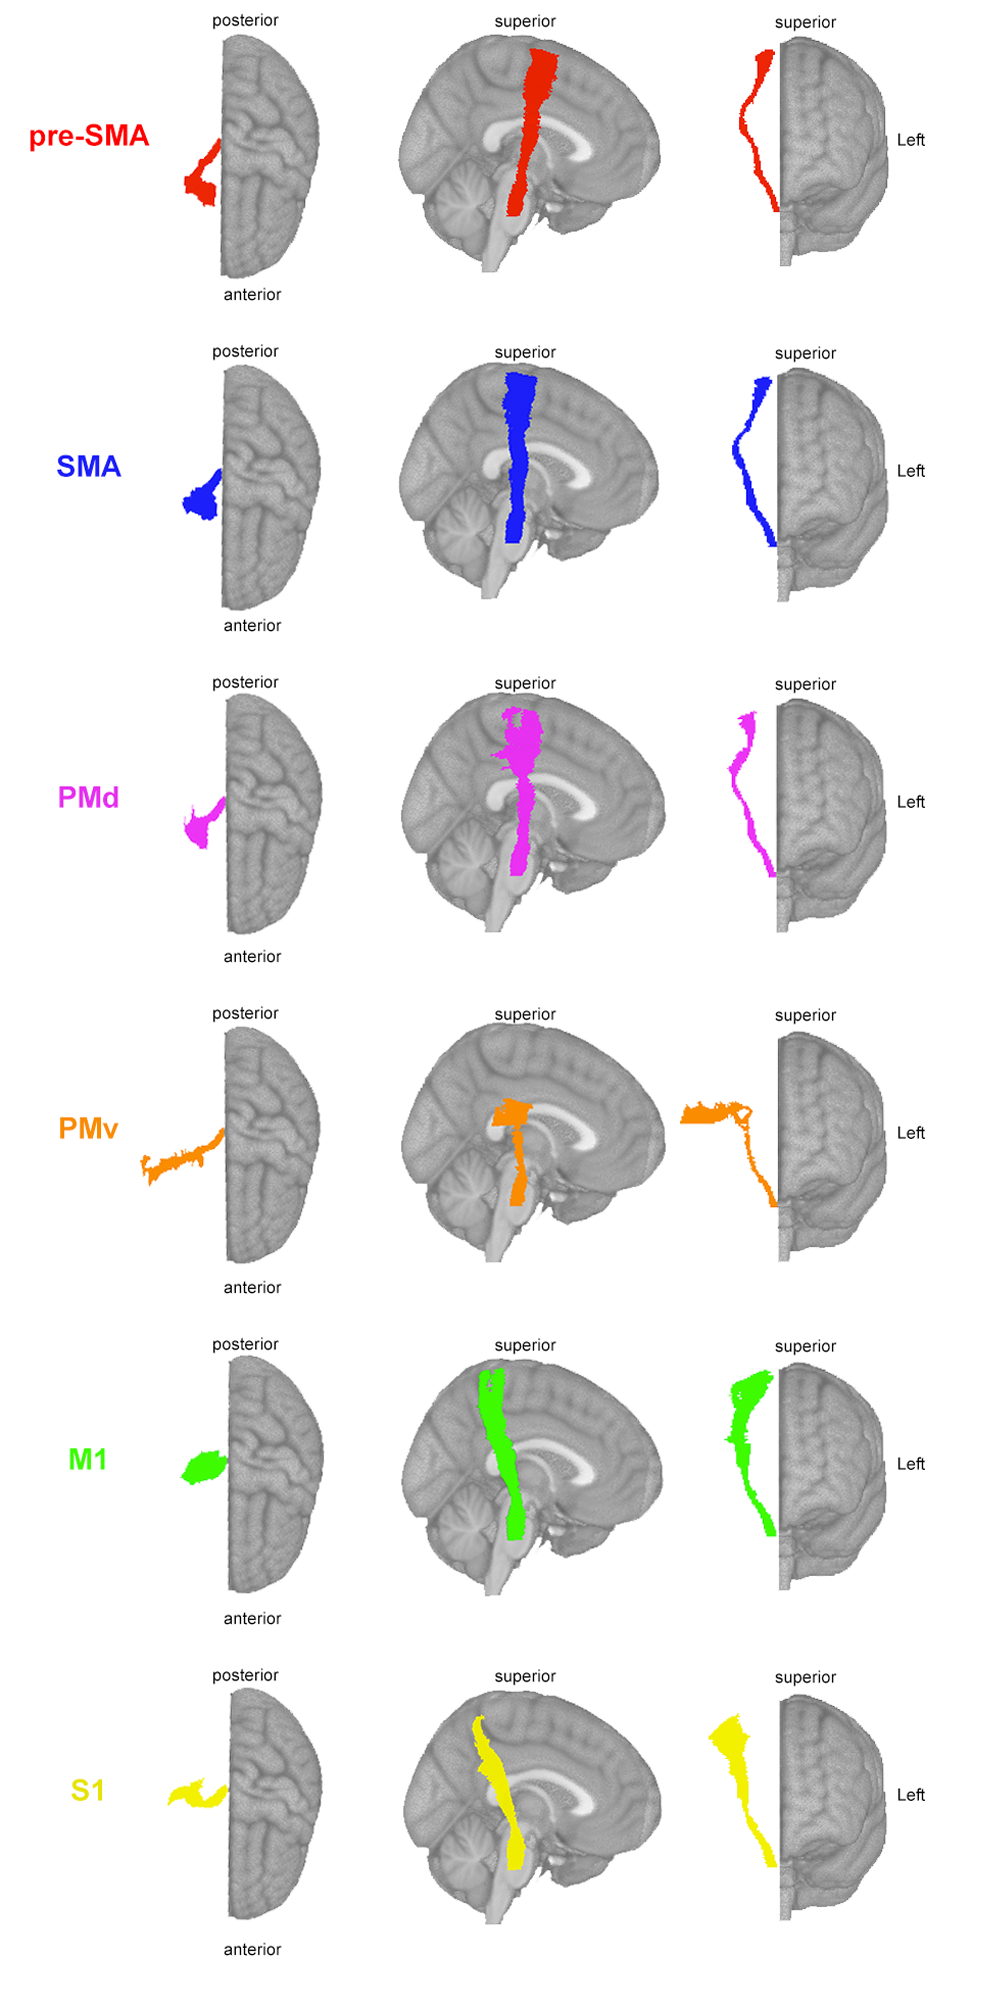
\includegraphics[width=1\linewidth]{chapter3/SMATT.png}
   
    \caption{Sensorimotor tract template atlas (SMATT), displaying only right hemisphere tracts relative to an MNI template. Includes supplementary motor area (SMA), dorsal premotor cortex (PMd), ventral premotor cortex (PMv), pre-supplementary motor area (pre-SMA), primary sensory cortex (S1),  and primary motor cortex (M1). Pre-SMA is the most anterior tract, S1 is the most posterior tract.}
    \label{smatt}
\end{figure}

\begin{figure}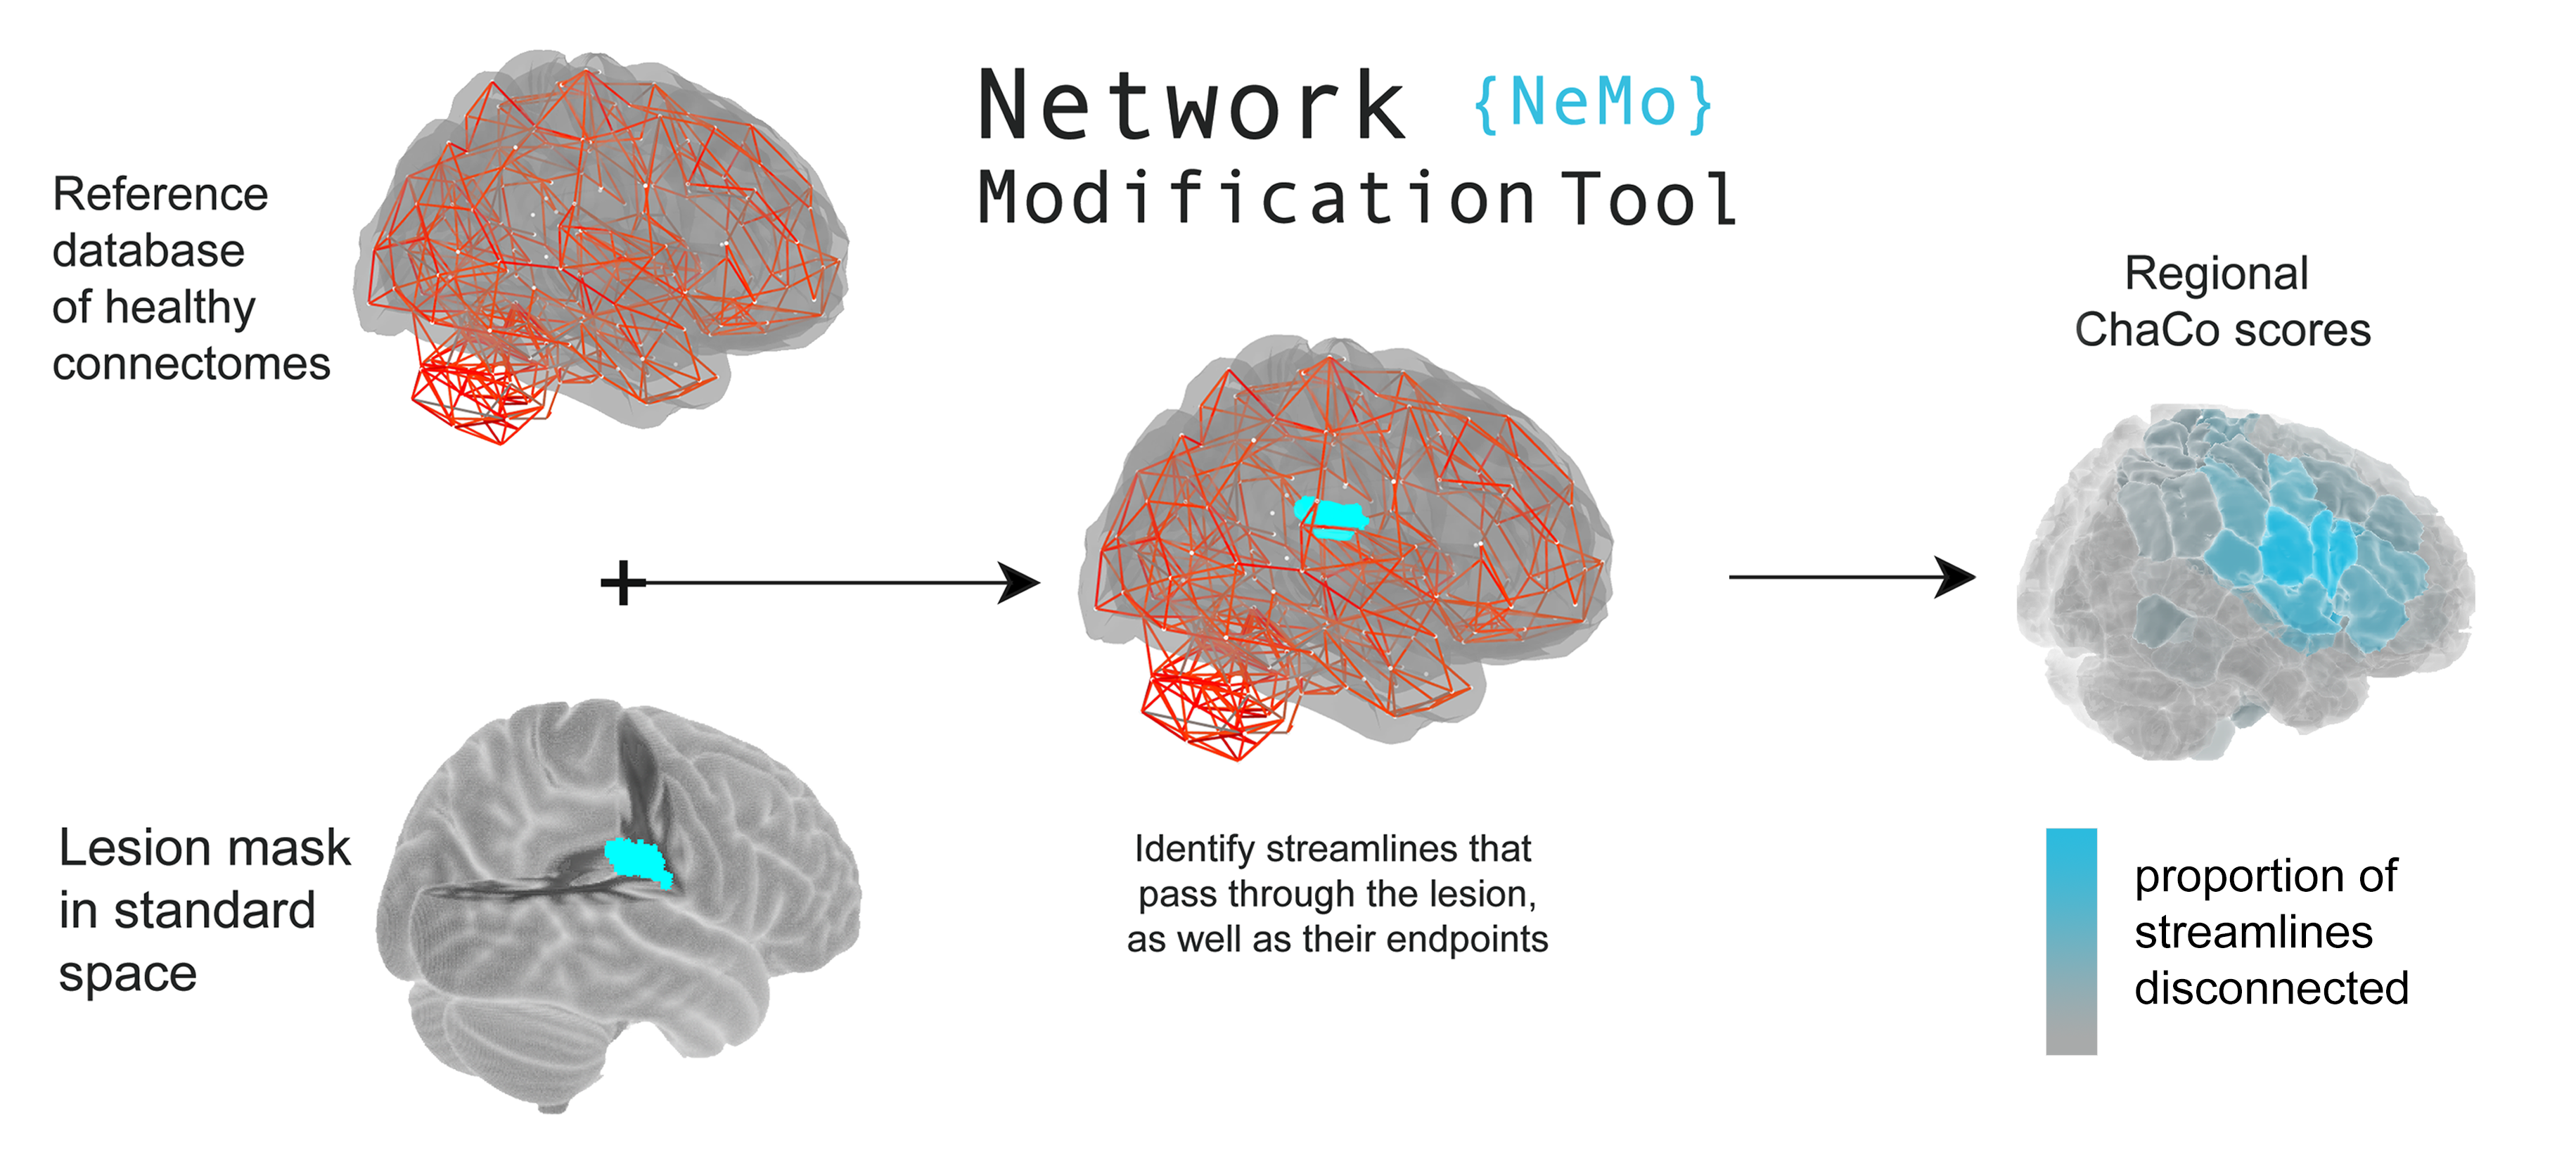
\includegraphics[width=1\linewidth]{chapter3/Multi-panelML_white_regional.png}
  \caption{Overview of the Network Modification tool. Binary lesion masks in MNI space representing the presence of a stroke lesion (turquoise) in a given voxel are provided by the user. Each lesion mask is embedded into 420 unrelated healthy structural connectomes (separately for each healthy subject) and the regional or pairwise change in connectivity (ChaCo) scores are calculated and averaged across healthy subjects (parcellation shown here is the Shen 268-region atlas). }
\label{chaco}
\end{figure}

Ridge regression models were used to predict chronic motor deficits from ipsilesional SMATT-LL (6 features) and from L/R-SMATT-LL (12 features). Ridge regression was used to account for multicollinearity of lesion load values between tracts (Supplementary Figure \ref{smatt_pairwise_correlations}, \ref{smatt_pairwise_correlations_bi}). Lesion load values were normalized (after train/test split) by subtracting the mean across subjects and dividing by the l2-norm prior to model fitting. In the inner loop, the degree of regularization on regression coefficients ($\lambda$) was determined via. grid-search, searching over 30 values ranging [$10^-2$ to $10^2$]. The training data was fit with the selected $\lambda$ and this model was used to predict motor scores for new subjects in the test folds.

\subsubsection{Structural lesion-network mapping (sLNM) models}
Structural lesion network maps were obtained from \cite{Bowren2022-rs}. Specifically, \cite{Bowren2022-rs} produced maps of white matter (WM) voxels in which damage predicted with Fugl-Meyer scores using sparse canonical corrleations analysis (\cite{Pustina2018-xv}). Then, tractography was seeded from those peak WM voxels to identify the structural networks associated with peak areas, which produced structural lesion network maps (sLNMs). Principal components analysis of sLNMs was performed, which produced 3 principal components that correspond to 5 sLNM maps (PC1, and positive/negative weights of PC2 and PC3 split). Lesion load on each sLNM map was calculated for each subject as the sum of the voxel intensities from the principal component map that also appeared within the boundaries of a lesion mask (Supplementary Figure \ref{slnm_distribution}). Ridge regression models were used to predict chronic motor deficits from sLNM lesion loads (5 features). As above, lesion load values were normalized (after train/test split) by subtracting the mean across subjects and dividing by the l2-norm prior to model fitting. In the inner loop, the degree of regularization on regression coefficients ($\lambda$) was determined via. grid-search, searching over 30 values ranging [$10^-2$ to $10^2$]. The training data was fit with the selected $\lambda$ and this model was used to predict motor scores for new subjects in the test folds. 

\subsubsection{Regional change in connectivity (ChaCo) models}
Lesion masks in $1mm^3$ MNI v6 space were processed with the Network Modification Tool (NeMo Tool) v2 pipeline (\cite{Kuceyeski2013-nk}) (https://github.com/kjamison/nemo for more detailed information). Given a lesion mask, the NeMo tool produces outputs that reflect the impact of the lesion on white matter tracts on the brain using healthy structural connectomes as a reference. The NeMo tool embeds a lesion mask into healthy structural connectomes, identifies all white matter streamlines that intersect with the lesion, and determines the brain regions at the endpoints of those streamlines (Figure \ref{smatt_and_chaco}B). Regional change in connectivity (ChaCo) scores, or the ratio of the number of disrupted streamlines divided by the total number of streamlines terminating in each region, were calculated for all gray matter regions (see Supplementary Figure \ref{mean_std_chaco}A,B for distribution of mean and standard deviation of ChaCo scores). The NeMo tool uses structural connectivity from 420 unrelated subjects from the Human Connectome Project Young Adult database. For each stroke lesion, the NeMo tool calcualtes regional ChaCo scores for all HCP subjects separately and then produces final regional ChaCo scores by taking the mean across HCP subjects. Structural connectivity in HCP subjects was obtained using deterministic tractography (SD stream) with dynamic seeding, with additional SIFT2 weighting for each of 5 million streamlines (\cite{Smith2015-eb}). Regional ChaCo scores from two different altases were compared: the 86-region Desikan-Killiany Atlas (68 cortical regions $\Plus$ 18 subcortical regions, excluding brainstem) from FreeSurfer ("fs86" for short), which contains coarse anatomically parcellated regions (\cite{Desikan2006-vf,Fischl2002-lb}), and the 268-region Shen atlas ("shen268" for short), which contains more fine-grained functionally parcellated cortical and subcortical regions (\cite{Shen2013-zn}).

First, the performance of ridge regression models was assessed, as described above, with regional ChaCo scores as inputs (86 features for the fs86 atlas, 268 features for the shen268 atlas). Second, a filter-based feature selection step was added to ridge regression models to obtain a subset of features that were the most useful for prediction (\cite{Guyon2003-kj, Hall1999-qr, Pudjihartono2022-zg}). We mixed hyperparameter tuning and feature selection in the same step, considering the number of features as a hyperparameter itself. Features were ranked by their their association with the outcome variable (p-value from univariate correlation) . In the inner loop, both the amount of regularization on regression coefficients ($\lambda$) and the number of features to retain in the feature selection step ($\kappa$) were selected via. grid search. The $\lambda$ value was chosen by searching over 30 values ranging [$10^-2$ to $10^2$], and the $\kappa$ value was chosen by searching 30 values ranging from 5 to the maximum number of features possible (for fs86: 86, for shen268: 268) in base-2 steps. 

\subsubsection{Ensemble models}

We tested whether models including demographic information (age, sex, and days post stroke) alongside lesion data will perform better than models with lesion data or demographic data alone (i.e., variance explained from lesion data and demographic data is not redundant). We also assessed whether models including both lesion load and ChaCo scores will perform better than models with lesion load or ChaCo scores alone. The idea of ensemble learning is to build a single prediction model by combining the strengths of a collection of simpler base models; we used ensemble models that average predictions from different damage metrics (\cite{Hastie2001-or}).

Ensemble models were generated by training ChaCo-models and lesion load models separately, on the same subjects and with the same training/test/validation splits, and averaging the final predicted scores for each subject. A standard linear regression model was used to model the relationship between demographic information and motor impairment. 

\subsubsection{Model comparisons}
Differences in performance between models were assessed using two-sided Mann-Whitney U tests. P-values were corrected for multiple comparisons using the Bonferroni correction. 

\subsubsection{Consistency of feature weights}
The stability of the beta coefficients for the best-performing models was assessed as follows. For the 86-region ChaCo models, the average of the 86-region weight vector across 5 folds was calculated for each permutation. This represents the average beta weights of the 5 best-performing models across cross-validation splits. The distribution of the average beta coefficients of all features across 100 permutation was plotted. For the 268-region ChaCo models with feature selection, the most consistently-selected features (selected in at least 475/500 folds or 99$\%$ of folds, heuristically) were identified and the average of those features across 5 folds was calculated for each permutation. This was done because the stability of features that were not consistently selected (which effectively have a weight of 0 in the model) was not relevant. The distribution of the average beta coefficients of consistently-selected features across 100 permutations was plotted. 

\subsubsection{Code availability}
All analysis scripts that generated the results of the present study are readily accessible and open for reuse (https://github.com/emilyolafson/lesion$\_$predictions). The script can be easily modified to predict any outcome score from ChaCo scores/lesion load data.

\subsection{Results}


\begin{figure}[htp]
\centering
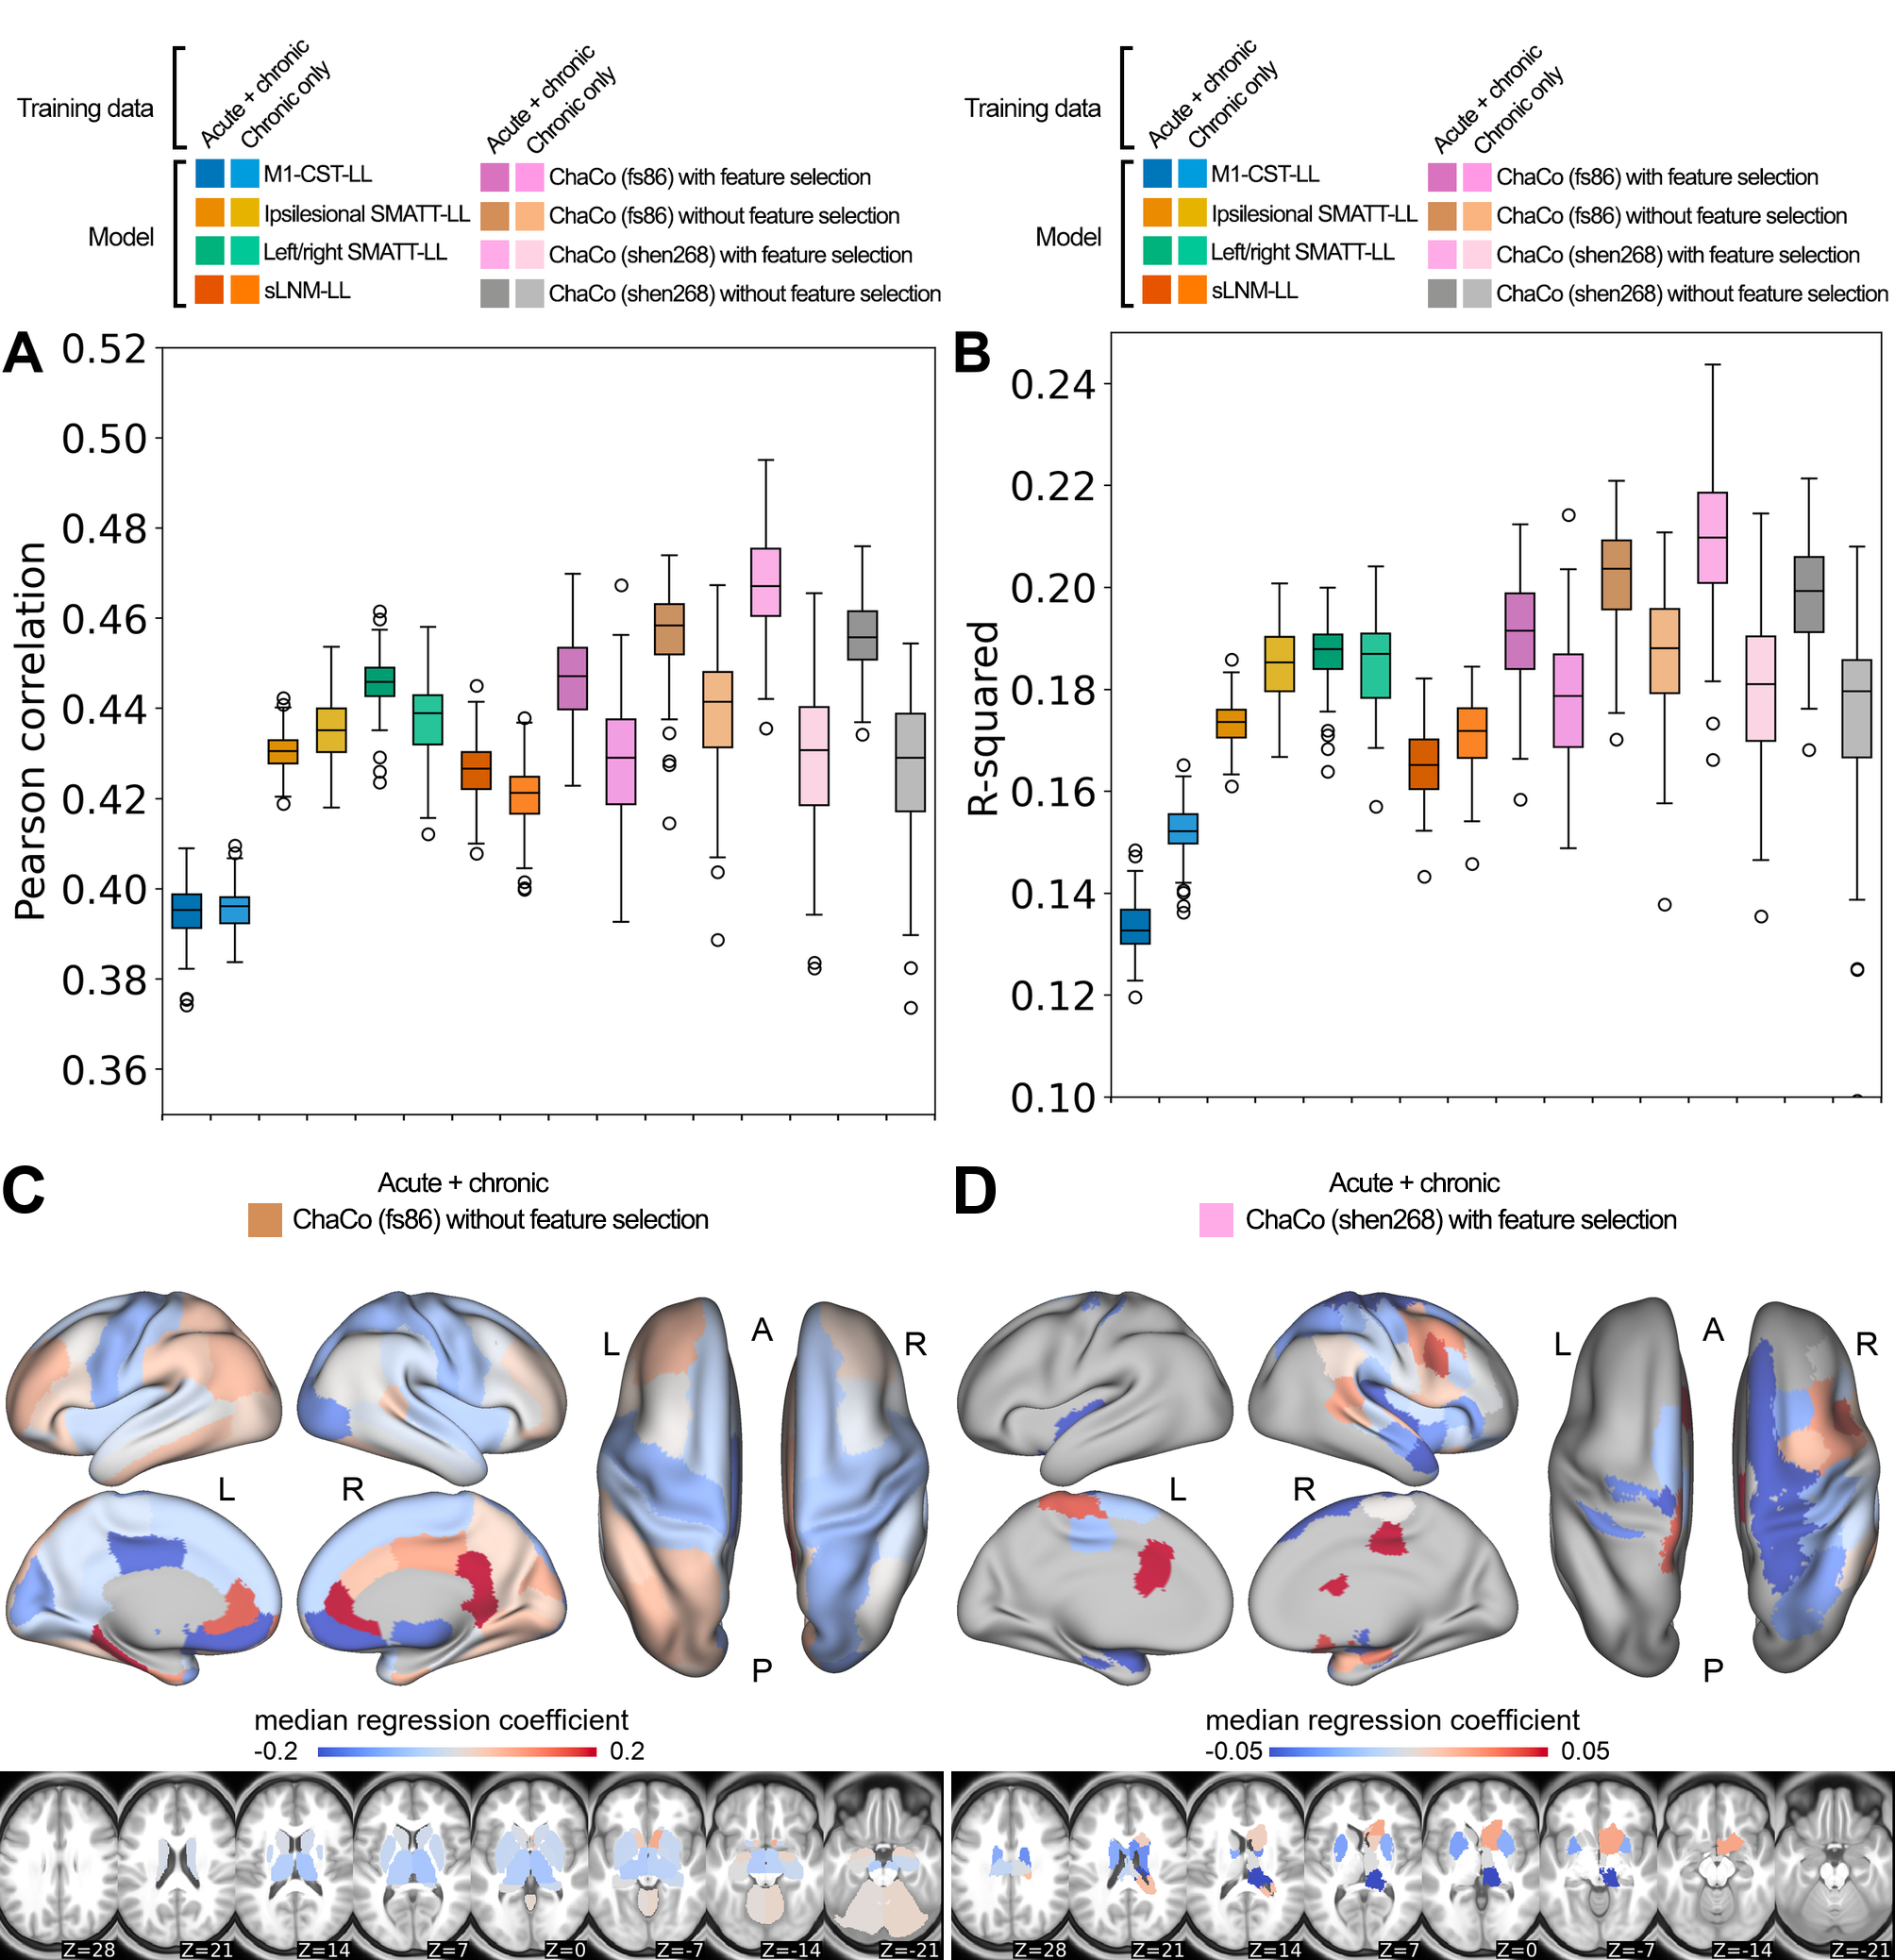
\includegraphics[width=1\linewidth]{chapter3/Figure1.png}
\caption{Summary of model performance metrics across all models tested and feature weights (regression coefficients) for best-performing models.  \textbf{A.} and \textbf{B.} Distribution of model performance (mean Pearson correlation/$R^2$ across 5 outer folds for 100 permutations of the data).  Boxplots are colored abritrarily for clarity and are plotted in similarly-colored pairs to indicate performance using the full training data ("Acute $\Plus$  chronic") versus only chronic data ("Chronic only"). The boxes extend from the lower to upper quartile values of the data, with a line at the median. Whiskers represent the range of the data from [Q1-1.5*IQR, Q3+1.5*IQR].
\textbf{C.} and \textbf{D.} Mean feature weights for the top 2 best-performing models (ChaCo (fs86) without feature selection, ChaCo (shen268) with feature selection, respectively). For fs86-ChaCo (left), displaying mean regression coefficients across 100 permutations. For ChaCo (shen268) (right), displaying median regression coefficients of regions that were selected in at least 95$\%$ of outer folds (i.e., for regions that were included in the model in at least 475/500 outer folds, means beta coefficients were calculated across 5 outer folds, and the median value across 100 permutations is plotted). }
\label{Figure3_1}
\end{figure}

The relative out-of-sample performances of the models can be found in Figure \ref{analysis1}A,B. In general, M1 CST-LL, SMATT-LL, and sLNM-LL performed worse on average than ChaCo models, with Left/Right SMATT-LL models performing the best among them (correlation = 0.446, $R^2$ = 0.188) and M1 CST-LL models performing the worst (correlation = 0.395, $R^2$ = 0.133, n.d. between chronic and mixed training data). 

Regional ChaCo scores from the 268-region Shen atlas best predicted chronic motor scores in unseen subjects. In particular, the best performance with this model was obtained using acute and chronic data for training as well as a feature selection step to identify a subset of relevant features (correlation = 0.467, $R^2$ = 0.210). Beta coefficients for selected features were consistent in direction and magnitude across permutations (Supplementary Figure \ref{shen_beta_coeffs})). The performance of this model was on par with a model using regional ChaCo scores from the 86-region FreeSurfer atlas, that also used acute and chronic data for training (correlation = 0.458, $R^2$ = 0.204, n.d. between models). Beta coefficients for all regions were consistent in direction and magnitude across permutations (Supplementary Figure  \ref{shen_beta_coeffs})).  Thus, the effect of feature selection in ChaCo models depended on the atlas: for the 86-region FreeSurfer atlas, feature selection reduced model performance, whereas for 268-region Shen atlas, model selection improved it. 

Model weights for the best-performing ChaCo models are shown in (Figure \ref{analysis1}C, D), reflecting median beta coefficients for regions selected in least 475/500 outer folds of the 268-region ChaCo models. There were several spatial similarities in the pattern of feature weights for the 86-region ChaCo model and 268-region ChaCo model with feature selection. For both atlases, negative model weights are assigned to superior portions of left and right motor areas, as well as in subcortical structures like the putamen, pallidum, and thalamus, whereas positive weights are assigned to frontal and parietal areas. In then 268-region ChaCo models, more regions in the right hemisphere are consistently included in the model than the left hemisphere. 



For ChaCo models using the shen 268-region atlas with feature selection, on average 110 features were selected (Supplementary Figure \ref{lambda_kappa}). A hierarchically-clustered heatmap of the correlation matrix of the selected features (Supplementary Figure \ref{heatmap_shen_negweights}) shows that many of the selected features are clustered (i.e., high correlation in ChaCo scores across subjects), and are frequently damaged together. Additionally, ChaCo scores of regions with positive and negative regression weights were positively correlated across subjects, despite these features having opposite relationships to motor deficits (Supplementary Figure \ref{heatmap_shen_pos_vs_negative}). For ChaCo models using the FreeSurfer 86-region atlas with feature selection, in the majority of cross-validation folds, all 86 regions were selected in the model. 

Including additional acute subjects in the training data improved model performance for Left/right SMATT-LL model and for ChaCo models. However, performance remained the same or was reduced for M1-CST-LL models, ipsilesional SMATT-LL models and sLNM models.

Generally, ensemble models performed marginally better than individual models. In particular, including demographic information increased or did not change prediction accuracy for all models tested, and combining ChaCo models with lesion load models improved performance. (L/R SMATT-LL + ChaCo (shen268) w/ feat. select $R^2 = 0.233$) above either alone (L/R SMATT-LL $R^2=0.188$, ChaCo (shen268) w/ feat. select, $R^2=0.210$)

Model weights for the best-performing models of each type are publicly available on GitHub. 


\newpage 
\newpage

\begin{table}[h]
\centering
\label{table:5}
\begin{tabular}{lrrll}
\toprule
 &  & \multicolumn{2}{c}{Median performance} \\
Ensemble type & Model name & Correlation & $R^2$  \\
\midrule
\multirow[t]{8}{*}{None (Lesion load or} & M1 CST-LL & 0.395 & 0.133 \\
 ChaCo only)& Ipsi. SMATT-LL & 0.430 & 0.174 \\
 & L/R SMATT-LL & 0.446 & 0.188 \\
 & sLNM-LL & 0.427 & 0.165 \\
 & ChaCo (fs86) & 0.458 & 0.204 \\
 & ChaCo (shen268) & 0.456 & 0.199 \\
 & ChaCo (fs86) (feat. select.) & 0.447 & 0.191 \\
 & ChaCo (shen268) (feat. select.) & 0.467 & 0.210 \\
\multirow[t]{16}{*}{Lesion load $\Plus$} & M1 CST-LL + ChaCo (fs86subj) & 0.461 & 0.210 \\
 ChaCo & M1 SMATT-LL + ChaCo (shen268) & 0.463 & 0.211 \\
 & Ipsi. SMATT-LL + ChaCo (fs86subj) & 0.478 & 0.226 \\
 & Ipsi. SMATT-LL + ChaCo (shen268) & 0.481 & 0.228 \\
 & L/R SMATT-LL + ChaCo (fs86subj) & 0.481 & 0.227 \\
 & L/R SMATT-LL + ChaCo (shen268) & 0.481 & 0.228 \\
 & sLNM-LL + ChaCo (fs86subj) & 0.468 & 0.214 \\
 & sLNM-LL + ChaCo (shen268) & 0.472 & 0.217 \\
 & M1 CST-LL + ChaCo (fs86subj) (feat. select.) & 0.458 & 0.206 \\
 & M1 CST-LL + ChaCo (shen268) (feat. select.) & 0.469 & 0.217 \\
 & Ipsi. SMATT-LL + ChaCo (fs86subj) (feat. select.) & 0.476 & 0.223 \\
 & Ipsi. SMATT-LL + ChaCo (shen268) (feat. select.) & 0.485 & 0.233 \\
 & L/R SMATT-LL + ChaCo (fs86subj) (feat. select.) & 0.475 & 0.222 \\
 & L/R SMATT-LL + ChaCo (shen268) (feat. select.) & 0.486 & 0.232 \\
 & sLNM-LL + ChaCo (fs86subj) (feat. select.) & 0.462 & 0.208 \\
 & sLNM-LL + ChaCo (shen268) (feat. select.) & 0.474 & 0.222 \\
\multirow[t]{8}{*}{Demographics} & M1 CST-LL + demog. & 0.424 & 0.173 \\
 & Ipsi. SMATT-LL + demog. & 0.457 & 0.199 \\
 & L/R SMATT-LL + demog. & 0.462 & 0.203 \\
 & sLNM-LL + demog. & 0.452 & 0.191 \\
 & ChaCo (fs86) + demog & 0.471 & 0.203 \\
 & ChaCo (shen268) + demog & 0.468 & 0.204 \\
 & ChaCo (fs86) (feat. select.) + demog & 0.465 & 0.201 \\
 & ChaCo (shen268) (feat. select.) + demog & 0.481 & 0.215 \\
\multirow[t]{16}{*}{Lesion load $\Plus$} & M1 CST-LL + ChaCo (fs86subj) + demog. & 0.476 & 0.214 \\
 ChaCo $\Plus$ & M1 CST-LL + ChaCo (shen268) + demog. & 0.477 & 0.216 \\
 Demographics & Ipsi. SMATT-LL + ChaCo (fs86subj) + demog. & 0.492 & 0.230 \\
 & Ipsi. SMATT-LL + ChaCo (shen268) + demog. & 0.495 & 0.232 \\
 & L/R SMATT-LL + ChaCo (fs86subj) + demog. & 0.494 & 0.231 \\
 & L/R SMATT-LL + ChaCo (shen268) + demog. & 0.494 & 0.232 \\
 & sLNM-LL + ChaCo (fs86subj) + demog. & 0.484 & 0.222 \\
 & sLNM-LL + ChaCo (shen268) + demog. & 0.487 & 0.224 \\
 & M1 CST-LL + ChaCo (fs86subj) (feat. select.) + demog. & 0.472 & 0.212 \\
 & M1 CST-LL + ChaCo (shen268) (feat. select.) + demog. & 0.482 & 0.222 \\
 & Ipsi. SMATT-LL + ChaCo (fs86subj) (feat. select.) + demog. & 0.490 & 0.228 \\
 & Ipsi. SMATT-LL + ChaCo (shen268) (feat. select.) + demog. & 0.498 & 0.237 \\
 & L/R SMATT-LL + ChaCo (fs86subj) (feat. select.) + demog. & 0.490 & 0.229 \\
 & L/R SMATT-LL + ChaCo (shen268) (feat. select.) + demog. & 0.499 & 0.237 \\
 & sLNM-LL + ChaCo (fs86subj) (feat. select.) + demog. & 0.479 & 0.218 \\
 & sLNM-LL + ChaCo (shen268) (feat. select.) + demog. & 0.492 & 0.230 \\
 
\bottomrule
\end{tabular}
\caption{Test performance of all models evaluated, displaying median $R^2$ and median correlation of average hold-out performances (i.e. average across 5 outer folds) across 100 permutations. Demog. = demographics, Ipsi. = Ipsilesional, SMATT LL = sensorimotor tract template lesion load, L/R SMATT LL = left and right sensorimotor tract template lesion load, M1 CST LL = M1 corticospinal tract lesion load, ChaCo = Change in Connectivity, fs86 = FreeSurfer 86-region atlas, feat. select. = feature selection}
\label{results_table_acutechronic}

\end{table}






\begin{figure}[htp]
\centering
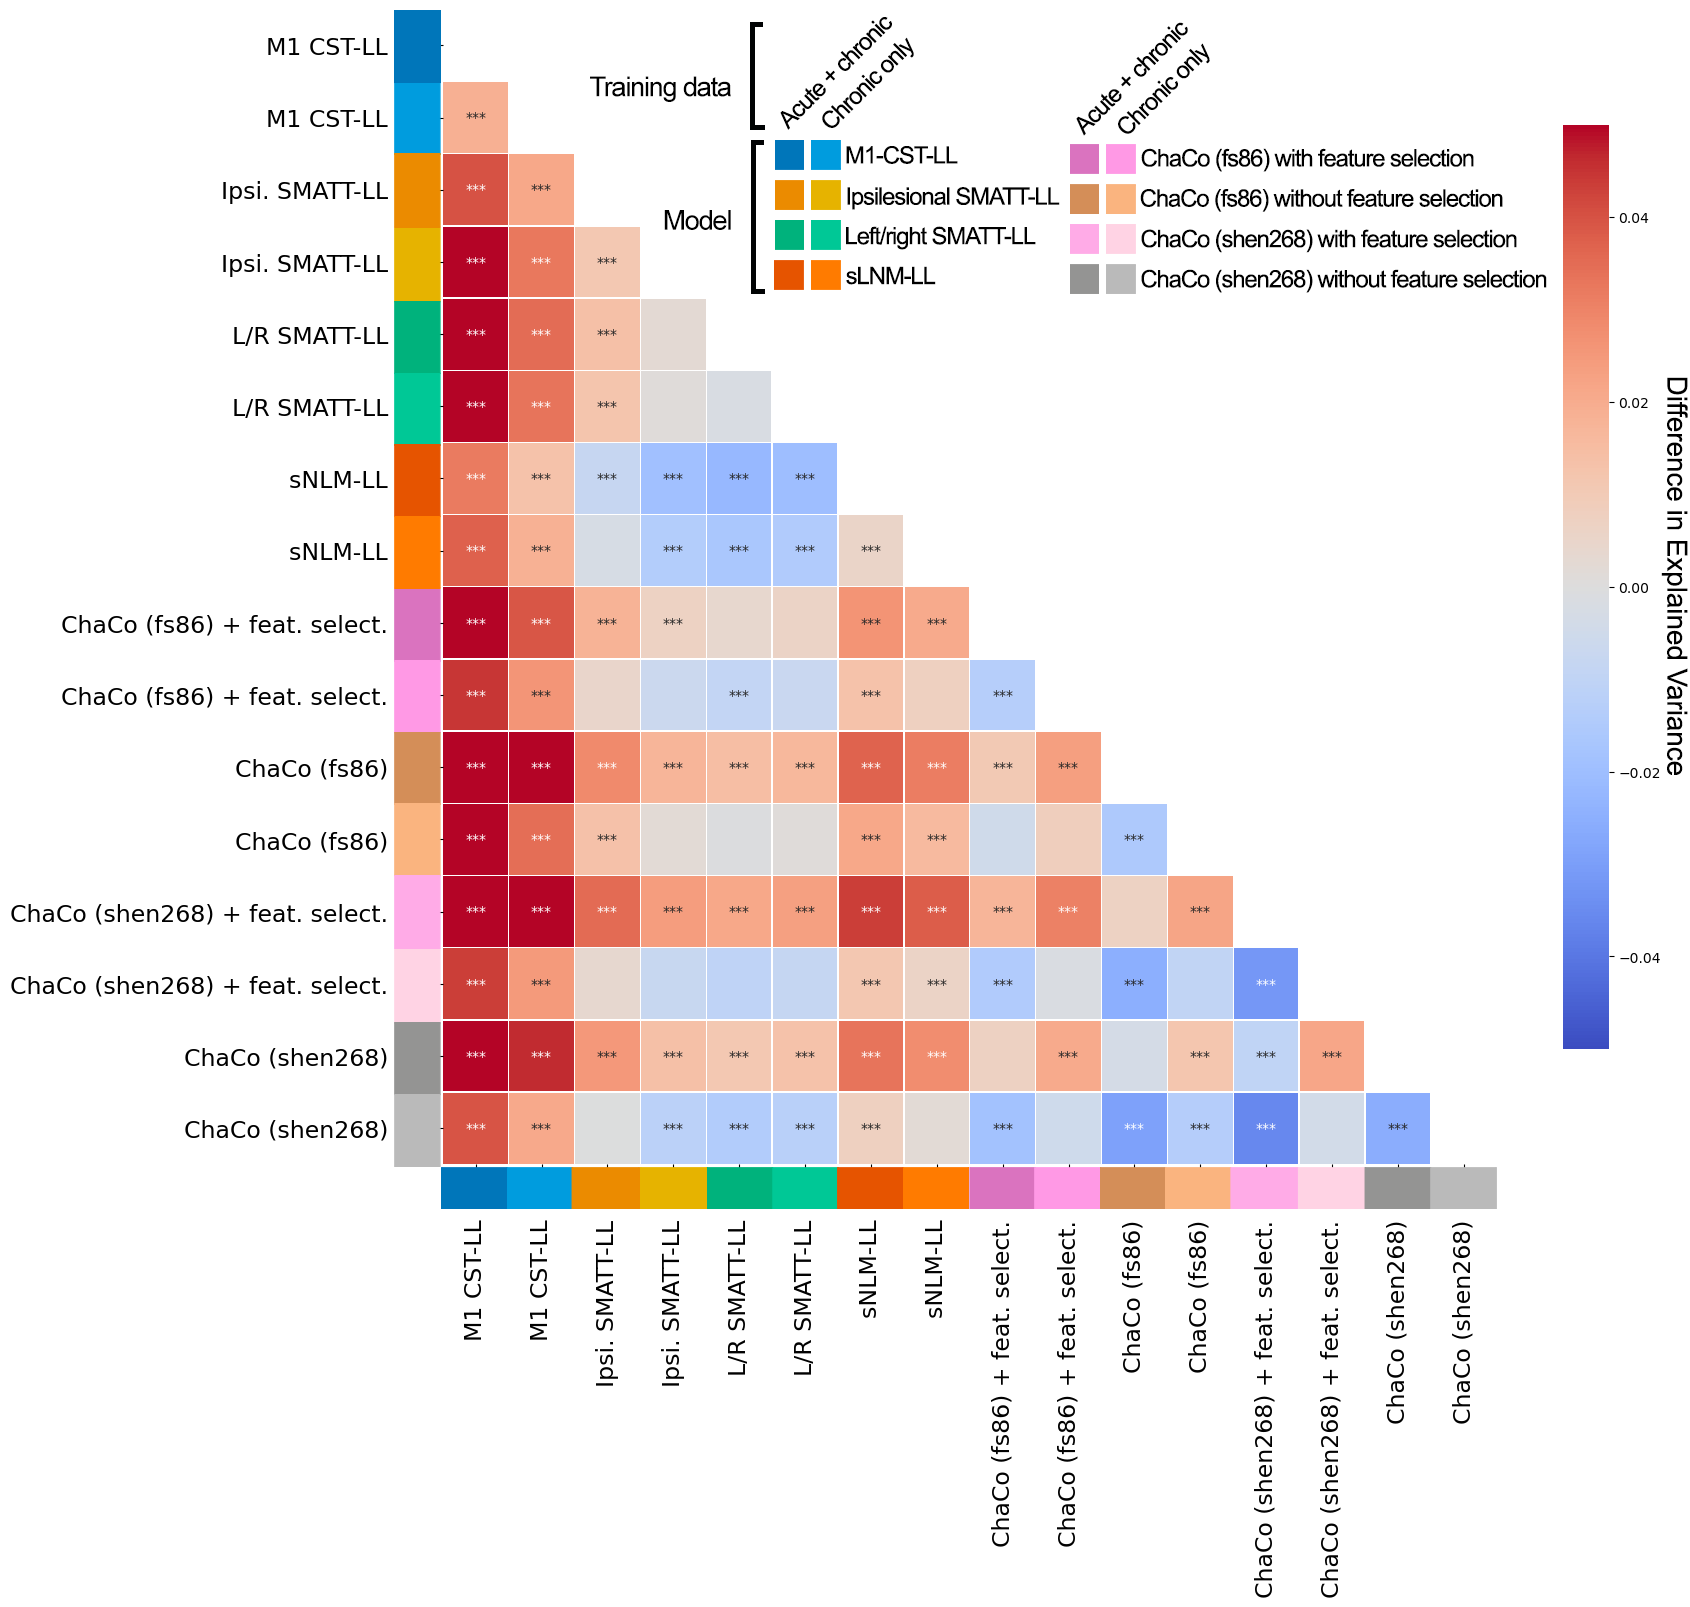
\includegraphics[width=1\linewidth]{chapter3/Figure2.png}
\caption{Significant differences in model performance for prediction of normalized motor scores. Difference in explained variance between pairs of models using different lesion metrics and different training data. Model differences were calculated by averaging the difference in explained variance for each of the 100 train/test splits. Significance of differences in explained variance were evaluated using exact tests for differences. $***$ denotes corrected $p < 0.001$, $**$ denotes corrected $p < 0.01$, $*$ denotes corrected $p < 0.05$ after Bonferroni correction. A positive difference value indicates that the model on the y-axis (vertical) has a greater explained variance than the model on the x-axis (horizontal).
 }
\label{Figure3_2}
\end{figure}

\begin{figure}[htp]
\centering
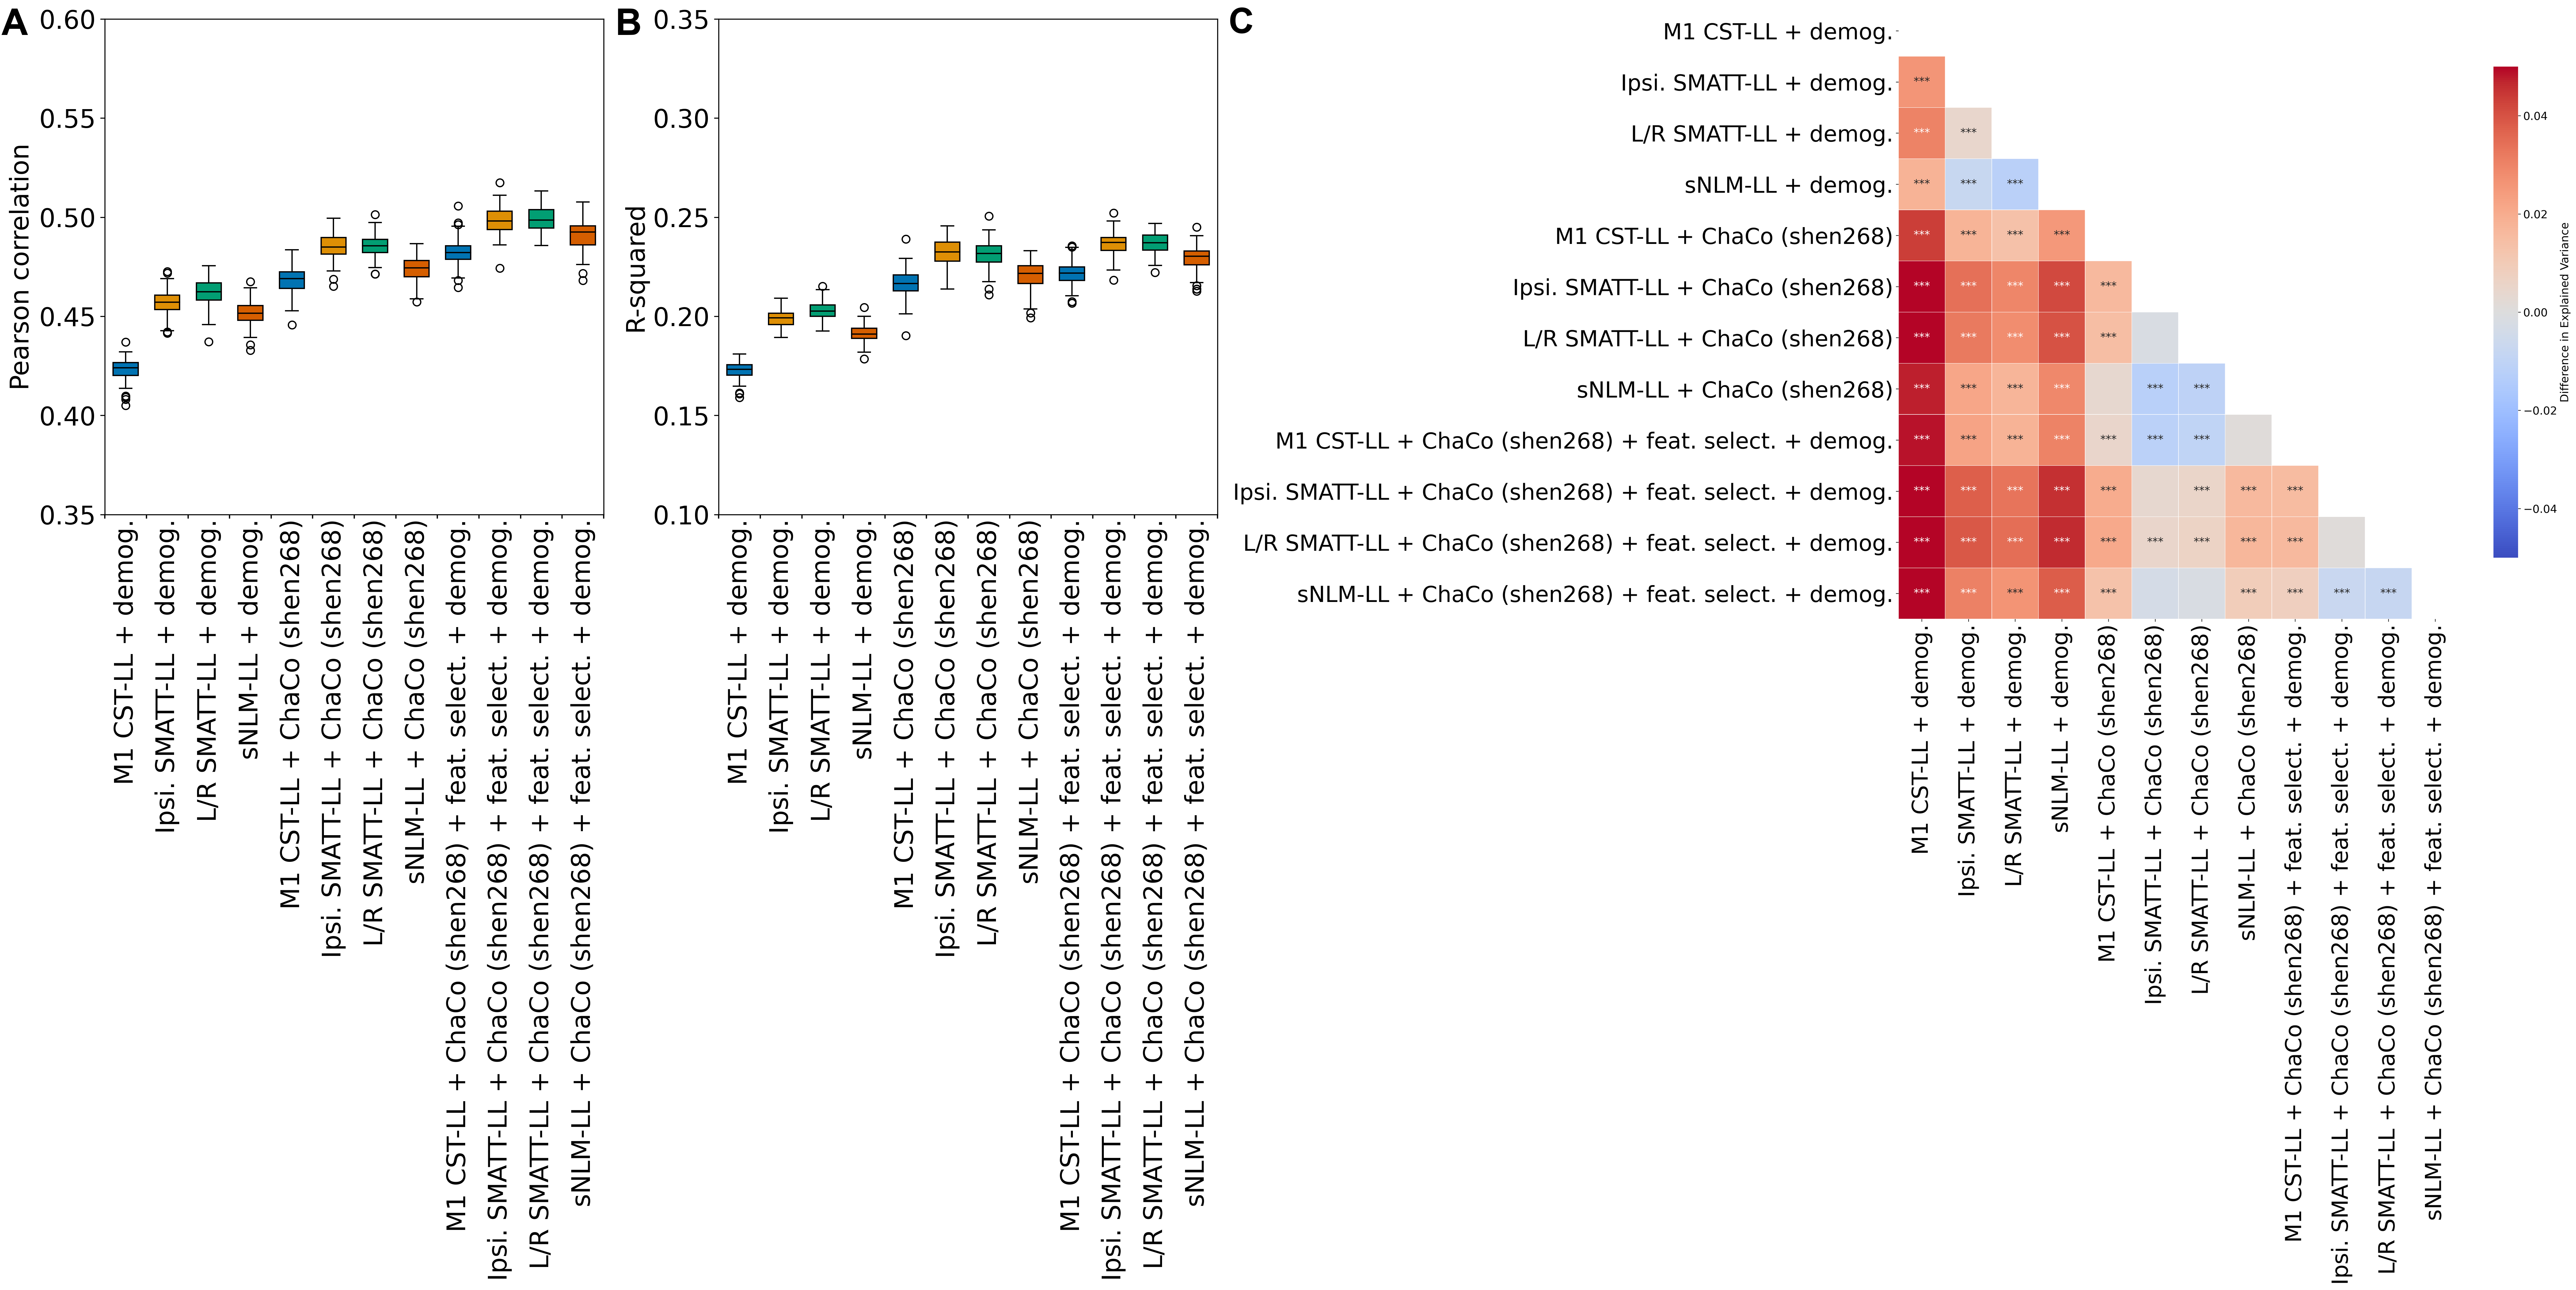
\includegraphics[width=1\linewidth]{chapter3/Figure3.png}
\caption{Ensemble model results. coefficients and model performance using Group KFold cross-validation (test/validate on independent imaging site). \textbf{A.} and \textbf{B.} display regression coefficients for regional ChaCo scores (FreeSurfer 86-region atlas, and Shen268-region atlas, respectively). Average feature weights for regions that were selected in at least half of the models (i.e., were included in the model in at least 250/500 outer folds). \textbf{C.} Sensorimotor area tract template feature importance for analysis 2. Includes primary motor cortex (M1), dorsal premotor cortex (PMd), ventral premotor cortex (PMv), supplementary motor area (SMA), pre-supplementary motor area (pre-SMA), primary sensory cortex (S1).}
\label{Figure3_3}
\end{figure}

\section{Discussion}
In this study, we assessed the relative predictive performance of several lesion metrics on the same large imaging dataset. We found that modelling lesion damage using regional ChaCo scores and using correlation-based feature selection best predicted chronic motor scores. Models using features derived from multivariate voxelwise lesion-behaviour modelling performed worse than more basic models using damage to parcellations of the descending corticospinal tract. Finally, we saw that combining several lesion metrics using ensemble modelling improved prediction performance, and that using acute stroke data to train models for prediction of chronic scores improved prediction performance. 

\subsubsection{M1-CST-LL vs. SMATT-LL: higher-order motor areas are relevant for motor outcome prediction}
This study supports previous results showing that M1-CST-LL alone does not capture enough variance to predict chronic motor outcomes in wide range of lesion topographies (\cite{Rondina2017-ij, Park2016-te, Ito2022-em}), although few studies have directly compared the out-of-sample performance of M1-CST-LL against more complex metrics like those assessed in this paper. Corticospinal projection tracts consist of fibers originating not just from M1, but from higher order motor areas in the frontal and parietal lobes (\cite{Galea1994-yi}) that have been implicated in motor planning and execution (\cite{Ball1999-yo}). Damage to descending fibers from these areas has been associated with motor deficits after stroke (\cite{Ito2022-em, Riley2011-xo}) and may explain additional variance in chronic motor outcome that is not captured by damage to M1 alone. Furthermore, preserving hemispheric information (i.e. in L/R SMATT-LL models) improved prediction performance above ipsilesional SMATT-LL, suggesting that there may be differential associations between motor tract damage and motor outcomes in each hemisphere. M1-CST-LL is currently the only structural neuroimaging biomarker recommended for clinical trials (\cite{Boyd2017-gs}); this study supports the notion that further development of non-M1-CST biomarkers is justified and that taking into account damage to multiple motor regions is important for understanding variation in motor outcome.

\subsubsection{Lesion-induced structural connectivity for prediction}

Models using ChaCo scores performed best of all models tested, specifically when feature selection was employed. ChaCo scores can can capture white matter and gray matter damage in one measurement (\cite{Kuceyeski2013-nk}), which may enable them to capture relevant associations between gray matter damage and motor deficits (\cite{Park2016-te,Rondina2016-ds}) that are not captured with lesion load metrics of tract damage. 

Another strength of models using ChaCo scores can be understood, in part, by considering its superior performance compared to sLNM models. One of the main differences between the features represented by the two models relates to when lesion-induced white matter damage is calculated. In both models, features reflecting lesion-induced damage are selected via optimization procedures on the basis of those features contributing to the prediction of motor deficits in a held-out sample; i.e., the features are selected in a data-driven way. However, in sLNM models, those features are voxels, and in ChaCo models, those features are regional ChaCo scores. Although sLNM identifies the white matter tracts that pass through voxels important for predictions and uses damage to those tracts as input to predictive models, the data on which feature selection takes place are voxels. False negatives may result from this type of modelling when partial damage of larger neural correlates produces a deficit (\cite{Sperber2022-oj}). Statistical power may be increased when voxelwise lesion data is instead transformed into regional ChaCo scores; non-overlapping lesions that affect different portions of the same tract are mapped onto ChaCo scores of the same region or set of regions. This data transformation essentially reduces the number of "rare" features compared to voxelwise representations, and can be qualitatively seen in the distribution of the standard deviation of ChaCo scores across subjects (Supplementary Figure \ref{mean_std_chaco}). The drawback to this approach is that regional ChaCo scores do not enable the detection of associations between damage to specific tracts and motor outcomes; if such associations exist then that signal may be diluted in regional measures. 

Although this is one of few studies to use regional structural disconnectivity measures to predict stroke outcomes (see also \cite{Tozlu2020-qa, Kuceyeski2016-vj}), it finds its conceptual home among voxelwise structural disconnection-behavior mapping approaches (\cite{Salvalaggio2020-pe, Wawrzyniak2022-kl, Foulon2018-bj, Sperber2022-oj}). Structural disconnection-behaviour mapping has been recently employed to identify white matter correlates of behaviour (\cite{Wawrzyniak2022-kl, Foulon2018-bj}), and to predict 2-week motor scores from lesion-induced structural disconnection (\cite{Salvalaggio2020-pe}). In the latter, most conceptually similar to this study, tractography is seeded from voxels in lesion and a map representing the probability of disconnection from the lesion is generated. Features for ridge regression models are generated via. principal components analysis (PCA) on the voxelwise structural disconnectivity maps. This is a reasonable dimensionality reduction step that has been applied in voxelwise lesion-symptom mapping (\cite{Ivanova2021-nh}), but is a fundamentally different approach to representing structural disconnection information than the Network Modification tool, which identifies the degree of disconnection for each brain separately. As demonstrated in this paper, regions that are frequently damaged together (and whose tracts may be loaded onto the same principal component in the PCA approach) may have opposite relationships to motor scores, so dimensionality reduction steps based on shared variance that do not consider relationships between structural disconnections and outcome variables (i.e. sCCA) may compress relevant individual signals into a single features, reducing the predictive performance of a model. 

\subsubsection{Features selected in ChaCo models}

In this paper, we are explicitly not attempting to do inference on the set of features that were selected by the model; however, further investigation into the features chosen along with their weights can provide some clarity into the model's performance. Correlation-based feature selection is known to choose redundant features (\cite{Guyon2003-kj})). Indeed, damage to many selected regions is highly correlated, suggesting that information from these regions is somewhat redundant. Does this mean that our model is suboptimal, and that fewer features are actually necessary for good predictions? No; in the context of lesion-deficit modelling, damage to adjacent regions can be highly correlated because they are supplied by the same vascular territory, and a stroke in that artery will cause damage to both areas (\cite{Mah2014-cb, Sperber2020-kp}). One may therefore expect that many regions share the same lesion-deficit association due to shared vasculature, and that damage to several areas, regardless of their causal relationship to hemiparesis, may be useful for predicting deficits. 

That feature selection identified such clusters of correlated damage is expected performance of the model based on the non-random distribution lesions and their relationship to deficits. Curiously, however, many regions whose white matter tracts are frequently damaged together (i.e. correlation in ChaCo scores across subjects $>$0.8) have opposite weights in the final regression model. Bona fide negative associations between damage and motor ability (or, identically, positive associations between damage and a deficit) are generally uncommon in lesion-deficit inference, though some cases of genuine facilitation have been documented (\cite{Kapur1996-xq, Sperber2020-kp}). These so-called paradoxical associations may arise when two regions are systematically not damaged together; if, for instance, individuals with posterior cerebral artery (PCA) stroke rarely have motor deficits, then damage to regions supplied by the PCA may be positively or only weakly associated with motor deficits (\cite{Sperber2020-kp}). We may therefore ask, in this study, why two regions whose white matter tracts \textit{are} systematically damaged together have opposite relationships to motor deficits? Likely, the large sample size and increased statistical power obtained by modelling structural disconnections instead of voxelwise damage enabled the model to identify differential lesion-deficit associations in areas that are frequently damaged together. That is, if region A and B are generally systematically damaged together but only A is related to hemiparesis, then without counter examples where only A or only B is damaged, it is impossible for the model to differentiate the two in terms of their association with a deficit. However, in a large sample, there may be enough counter-examples where only B is damaged and a subject does not have a deficit, or when only A is damaged and a subject does have a deficit, that the model assigns opposite weights to these areas. 


\subsubsection{Use of acute data in training}
Inclusion of the acute data improved predictions. Although in this paper we did not attempt to disentangle the effect of greater training size from relevance of the signal in the acute data, we can say that the acute data was, at the very least, not harmful for predictions of chronic motor scores. In particular, feature selection seemed to only improve performance when acute data was included in the training set. There is some helpful signal in this population, if the statistical relationships between lesion and deficits changed over the course of the stroke then this information may not be useful. Likely, unmeasured factors like structure and functional reorganization and lifestyle weaken the underlying relationship between lesion location and motor deficit as time between the stroke and the assessment increases (\cite{Shahid2017-gx}). 

We may also conclude that because of this shared variance and decreased signal-to-noise ratio in the chronic subjects, predictive performance in acute subjects may be thought of as an upper limit of performance achieveable on chronic data. 

\subsubsection{Ensemble models}
Finally, we saw that averaging predictions from multiple models improves performance above either model alone. This suggests that the information within each is not redundant, and that using multiple different lesion metrics may compensate for weaknesses of different feature representations. In this study, SMATT-LL models have the ability to distinguish between damage to several adjacent descending corticospinal tracts, but are unable to measure lesion-deficit associations outside this area, or in the gray matter. On the other hand, ChaCo models can detect associations across the entire brain and in the gray matter but may not have sufficient resolution between different branches of the corticospinal tract to capture relevant variance there. Beyond predictions of chronic motor scores, prediction models may be improved by testing and possibly combining various feature representations to obtain and optimal model (\cite{Kasties2021-rm}).

\subsubsection{Limitations}
There are several limitations of this study. Without baseline motor scores, we cannot evaluate the relative predictive power of lesion damage versus baseline behavioural information, which may share variance (\cite{Feng2015-du, Bowren2022-rs}). Since this information would likely be accessible for future clinical trials or prediction contexts, it is important to determine to what degree lesion information provides explanatory power above baseline motor scores, though previous studies have shown that prediction models with behavioural predictors and imaging biomarkers explain more variance in motor outcomes than the models with behavioural predictors alone (\cite{Kim2017-xe, Feng2015-du}). Second, the inclusion of metrics that are not specific to motor deficits (i.e. NIHSS) may have reduced sensitivity of models. Third,

This study compares only one type of lesion-behavior mapping technique 



\label{chap:3}
\appendix
\chapter{Supplementary material for Chapter 1}
\label{chap:4}

\null
\vfill
\begin{figure}[h!]

    \centering
    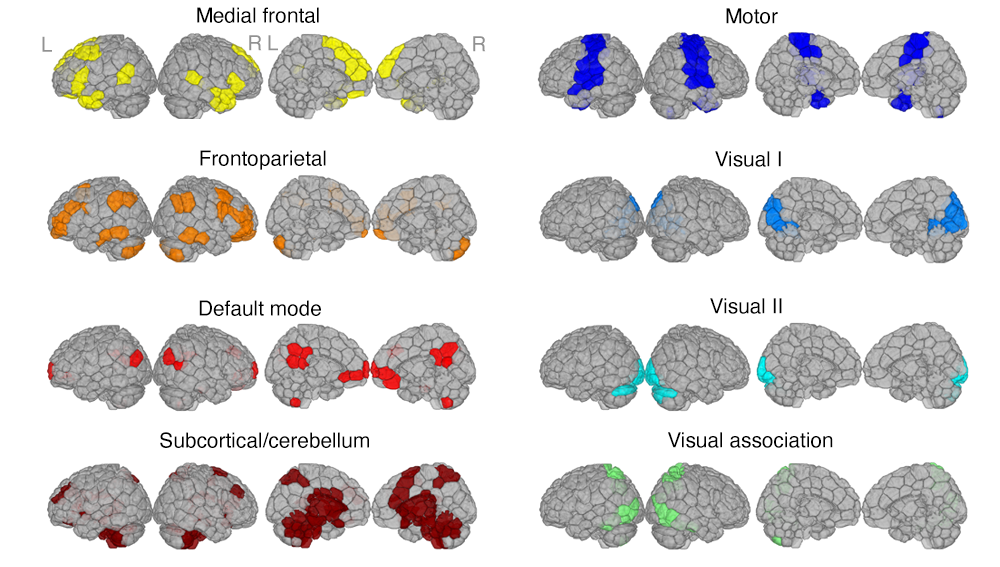
\includegraphics[width=\textwidth]{chapter1/SupplementaryFigure1.png}
       \caption{Functional network visualizations.}
  \caption*{8 functional networks identified by (\cite{Finn2015-er}) by clustering healthy functional connectivity matrices.}
      \label{SupplementaryFigure1}
\end{figure}
\null
\vfill



\clearpage
\null
\vfill
\begin{figure}[h!]
    \centering
    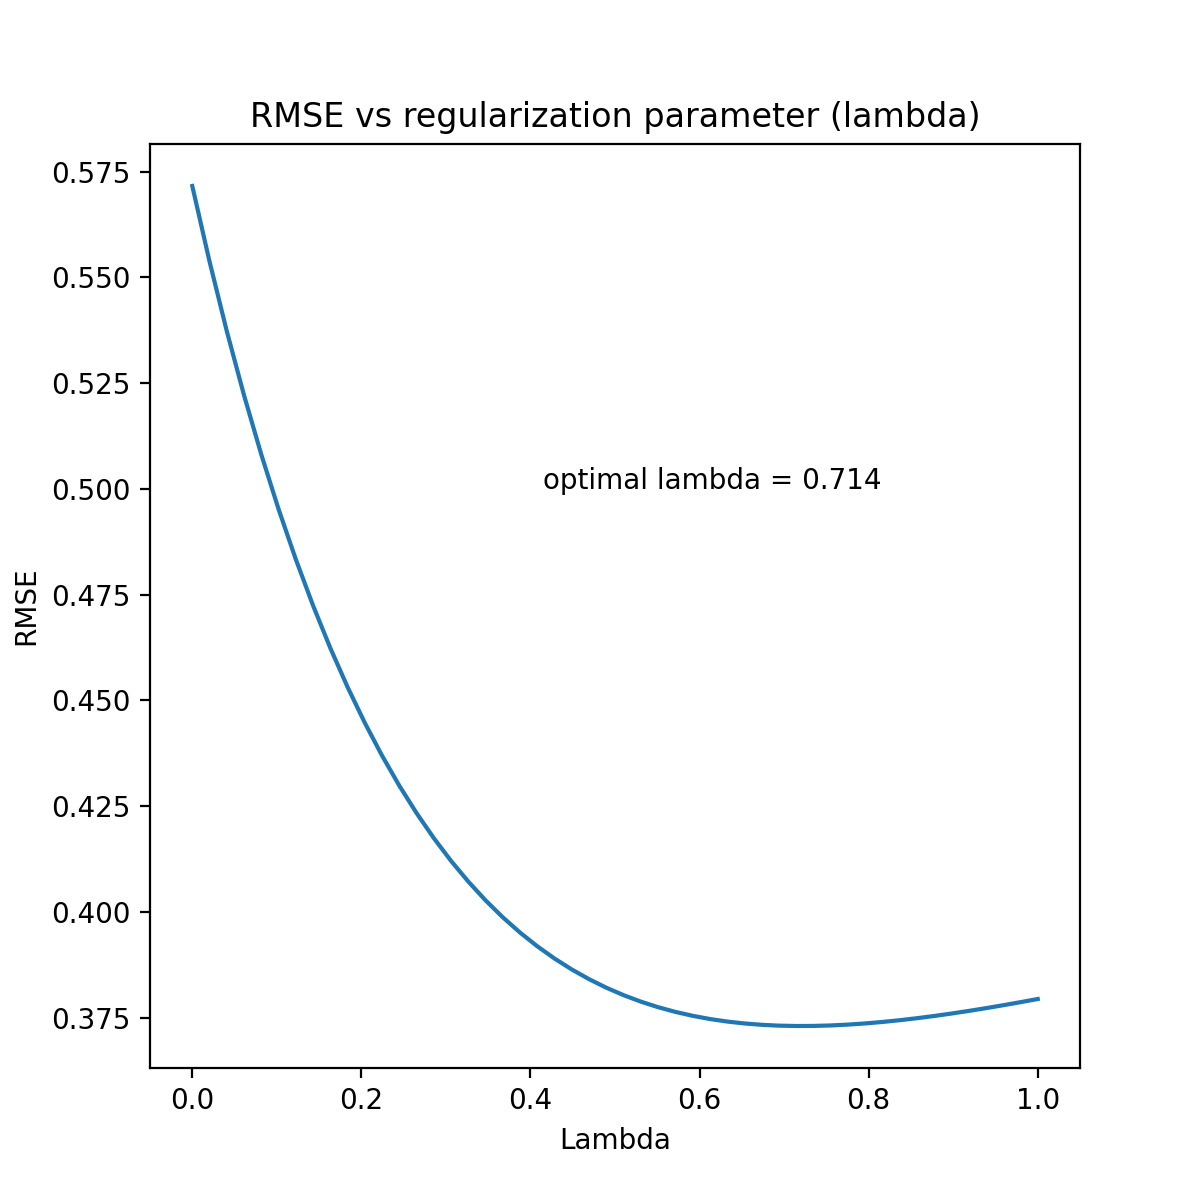
\includegraphics[width=\textwidth]{chapter1/SupplementaryFigure2.png}
       \caption{Results of optimization procedure to choose the best regularization parameter, lambda ($\lambda$).}
  \caption*{ The lambda that is chosen is the one that minimizes the root mean squared error of the Frobenius norm of the difference in regularized subject precision matrices $P_i^{reg}$ and the group average unregularized precision matrix $P_{avg}$, which was found to be $\lambda = 0.71$. }
      \label{SupplementaryFigure2}
\end{figure}
\null
\vfill


\clearpage
\null
\vfill
\begin{figure}[!hp]
\caption{Functional connectivity (node strength) differences between stroke and control subjects. }
\caption*{Significant differences and node strength (for a single node, node strength is the sum of connectivity weights to all other nodes), assessed with mass-univariate t-tests at each node  and corrected with Benjamini-Hochberg FDR correction. Left hemisphere is the leftmost brain; right hemisphere is the rightmost brain. Top row shows the lateral view, bottom row shows a medial view.}
    \label{SupplementaryFigure3}
\end{figure}
\null
\vfill
\clearpage
\null
\vfill
\begin{figure}[h!]
		\ContinuedFloat
		\captionsetup{labelformat=adja-page}
    \centering
    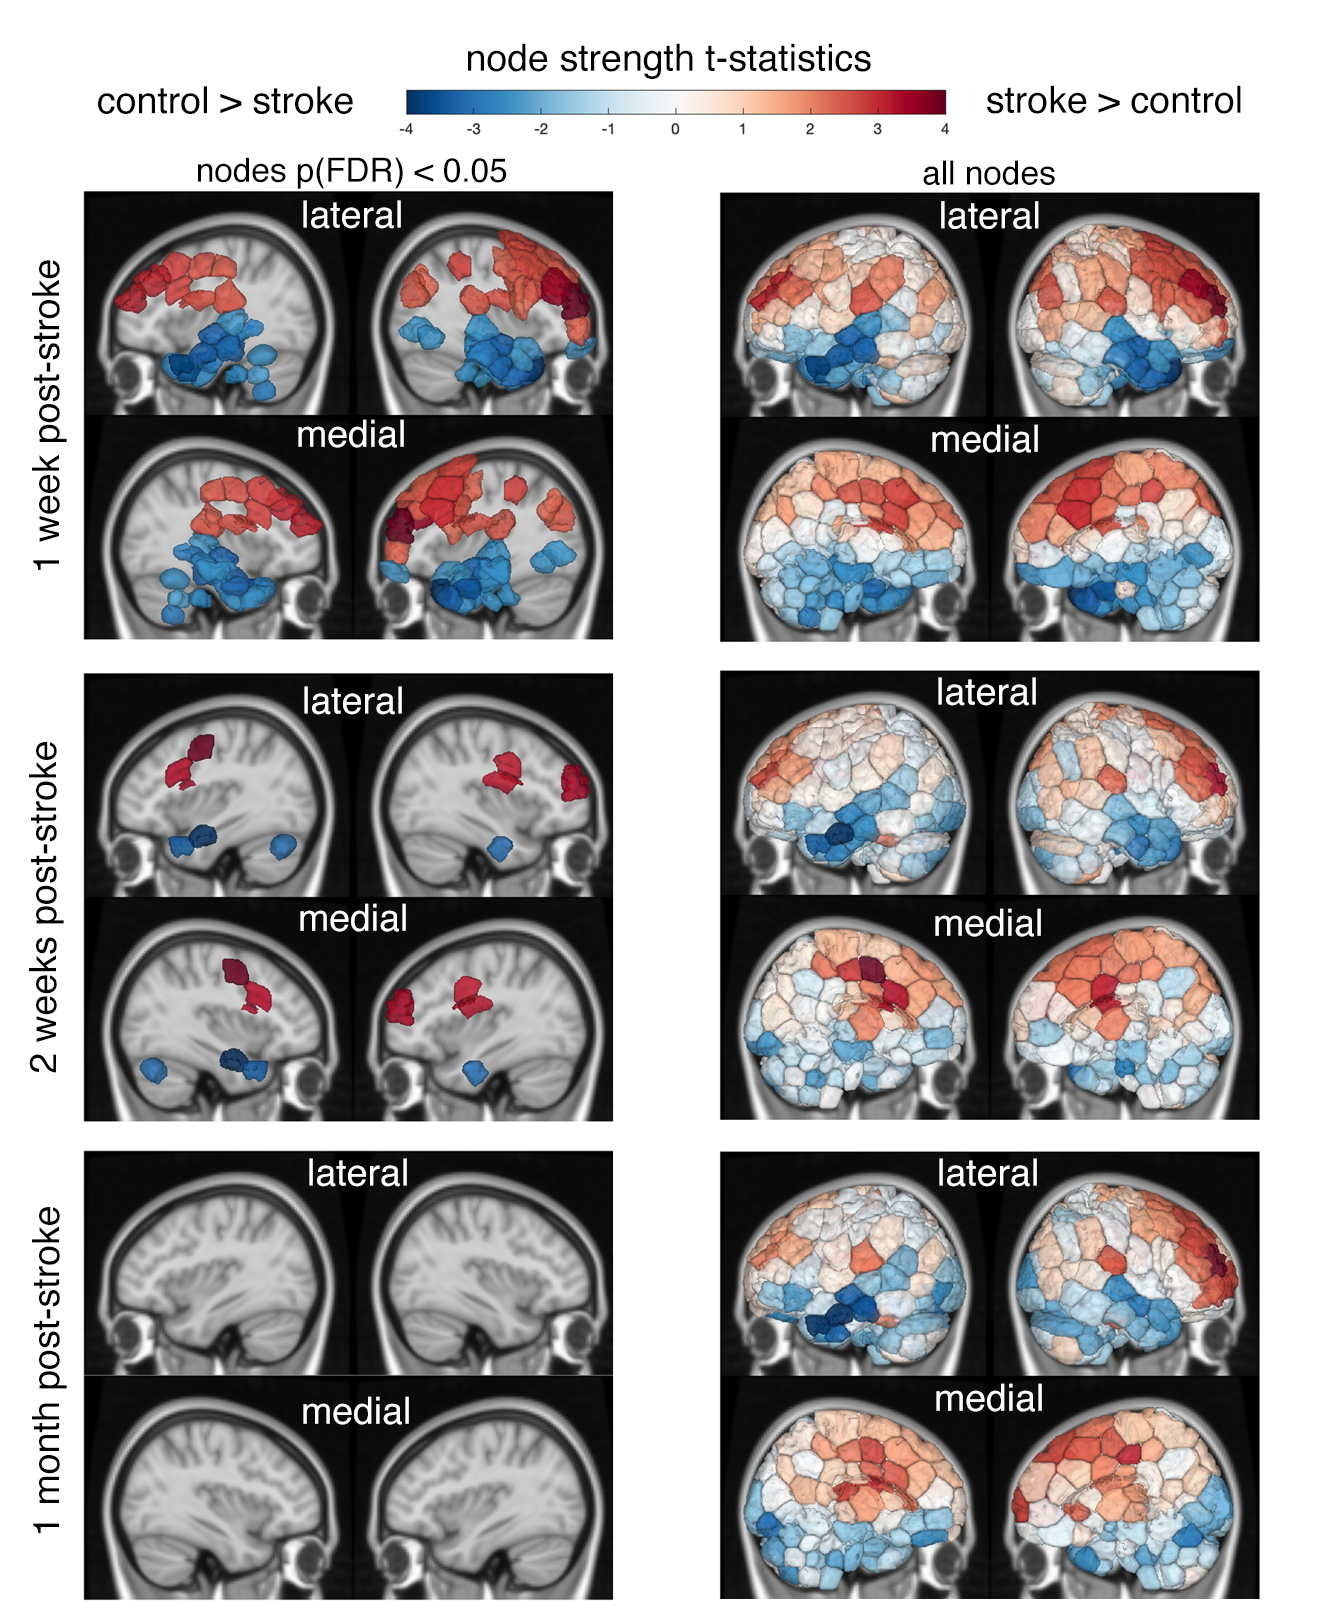
\includegraphics[width=\textwidth]{chapter1/SupplementaryFigure3_1.png}
    \caption[]{}
\end{figure}
\null
\vfill
\clearpage
\null
\vfill
\begin{figure}[h!]
		\ContinuedFloat
		\captionsetup{labelformat=adja-page}
    \centering
    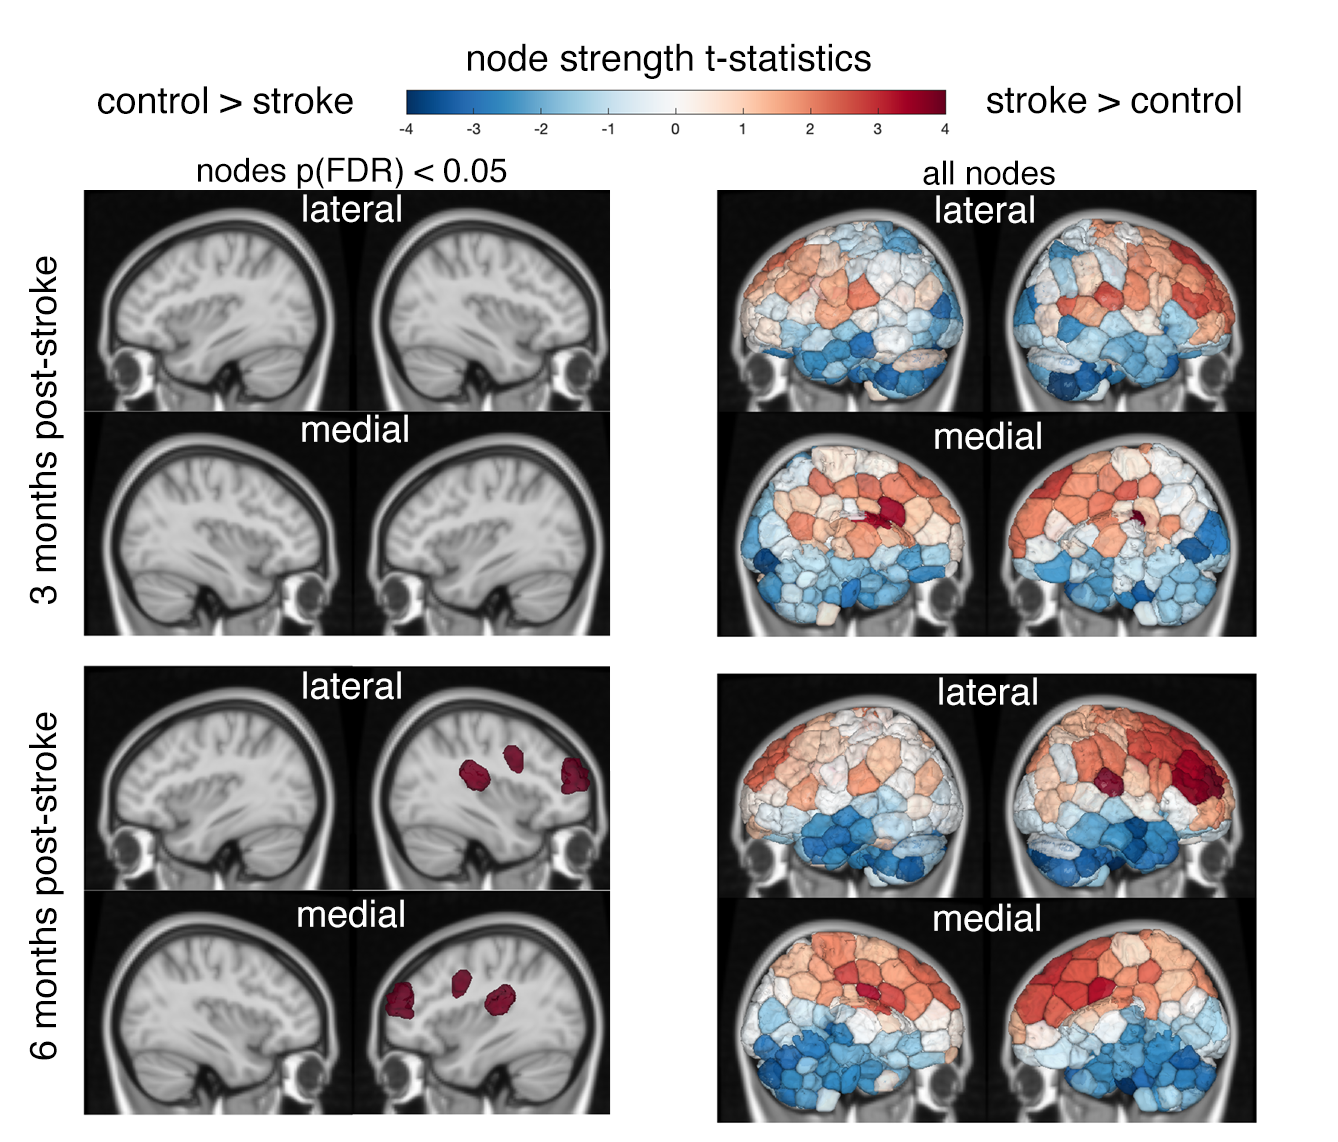
\includegraphics[width=\textwidth]{chapter1/SupplementaryFigure3_2.png}
    \caption[]{}
\end{figure}
\null
\vfill
\clearpage


\clearpage
\null
\vfill
\begin{figure}[!hp]
       \caption{Correlation between scan length (number of TRs after motion scrubbing) and remapping.}
  \caption*{Top row: correlation between the total number of remaps observed between time points (column) and the average scan length of the two time points. Middle row: correlation between the total number of remaps observed between the number of remaps and the scan length of the first time point (chronologically). Bottom row: correlation between the total number of remaps observed between the number of remaps and the scan length of the second time point (chronologically).}
    \label{SupplementaryFigure4}
\end{figure}
\null
\vfill
\clearpage
\null
\vfill
\begin{figure}[h!]
		\ContinuedFloat
		\captionsetup{labelformat=adja-page}
    \centering
    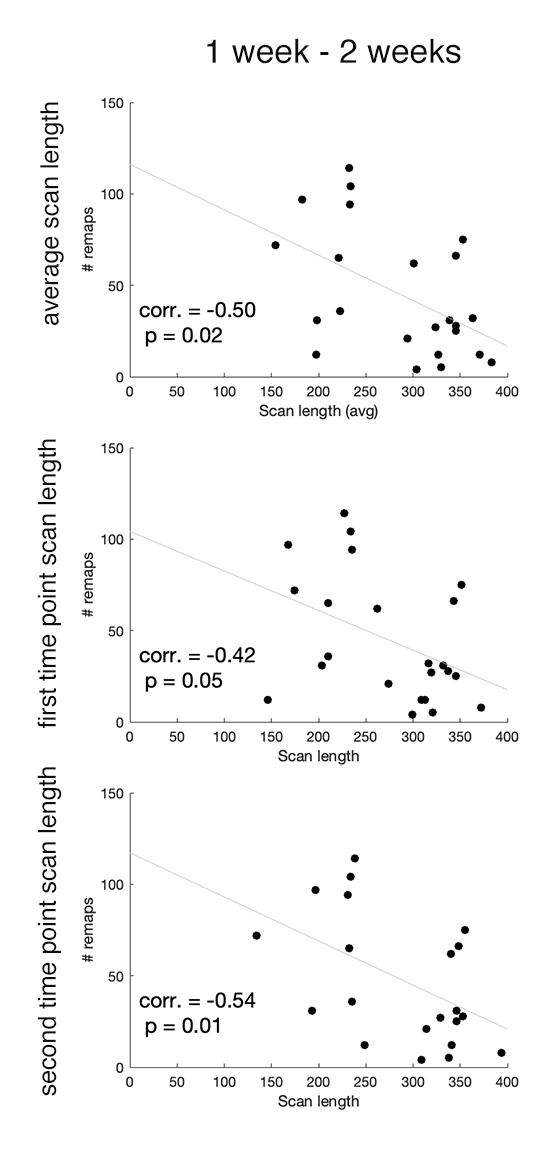
\includegraphics[width=0.60\textwidth]{chapter1/SupplementaryFigure4A.png}
    \caption[]{}
\end{figure}
\null
\vfill
\clearpage
\null
\vfill
\begin{figure}[h!]
		\ContinuedFloat
		\captionsetup{labelformat=adja-page}
    \centering
    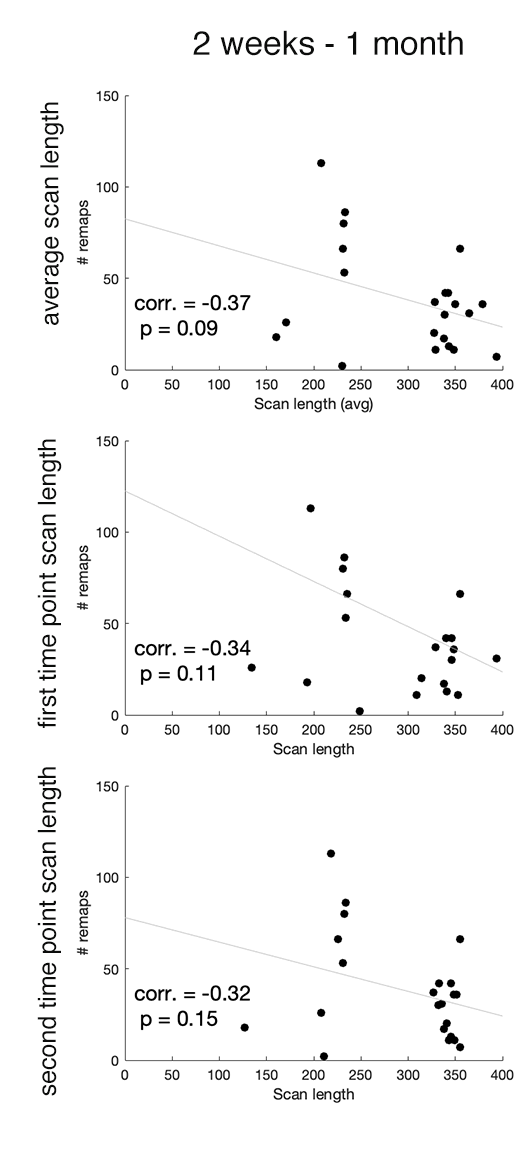
\includegraphics[width=0.6\textwidth]{chapter1/SupplementaryFigure4B.png}
    \caption[]{}
\end{figure}
\null
\vfill
\clearpage
\null
\vfill
\begin{figure}[h!]
		\ContinuedFloat
		\captionsetup{labelformat=adja-page}
    \centering
    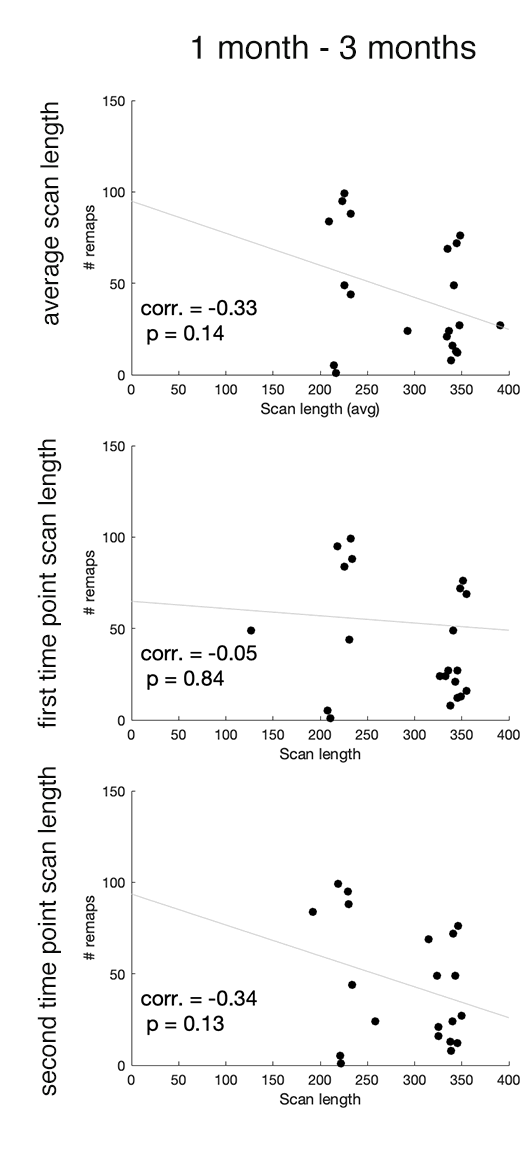
\includegraphics[width=0.6\textwidth]{chapter1/SupplementaryFigure4C.png}
    \caption[]{}
\end{figure}
\null
\vfill
\clearpage
\null
\vfill
\begin{figure}[h!]
		\ContinuedFloat
		\captionsetup{labelformat=adja-page}
    \centering
    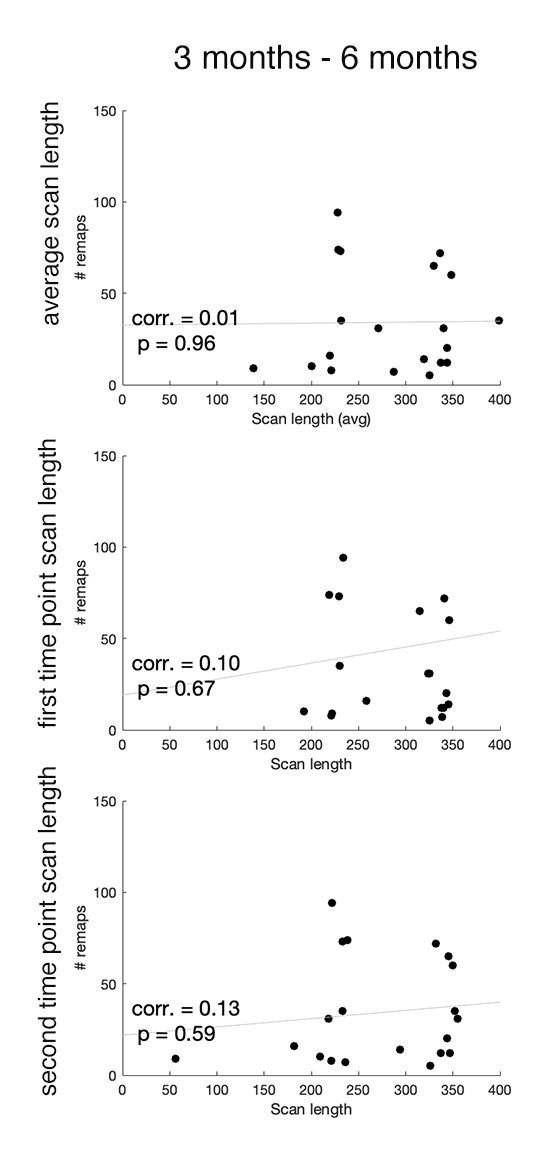
\includegraphics[width=0.6\textwidth]{chapter1/SupplementaryFigure4D.png}
    \caption[]{}
\end{figure}
\null
\vfill
\clearpage



\null
\vfill
\begin{figure}[!hp]
       \caption{Relationship between disconnection frequency and remapping frequency. }
  \caption*{Remapping preferentially occurs in regions with greater structural connectivity disruption \textbf{A.} Correlations between average ChaCo scores and regional remap frequencies across all 23 stroke subjects. Regions are colored by network assignment. \textbf{B.} Nodes that remap have a higher proportion of disconnected nodes than nodes that do not remap, for all time points.}
    \label{SupplementaryFigure5}
\end{figure}
\null
\vfill
\clearpage
\null
\vfill
\begin{figure}[h!]
		\ContinuedFloat
		\captionsetup{labelformat=adja-page}
    \centering
    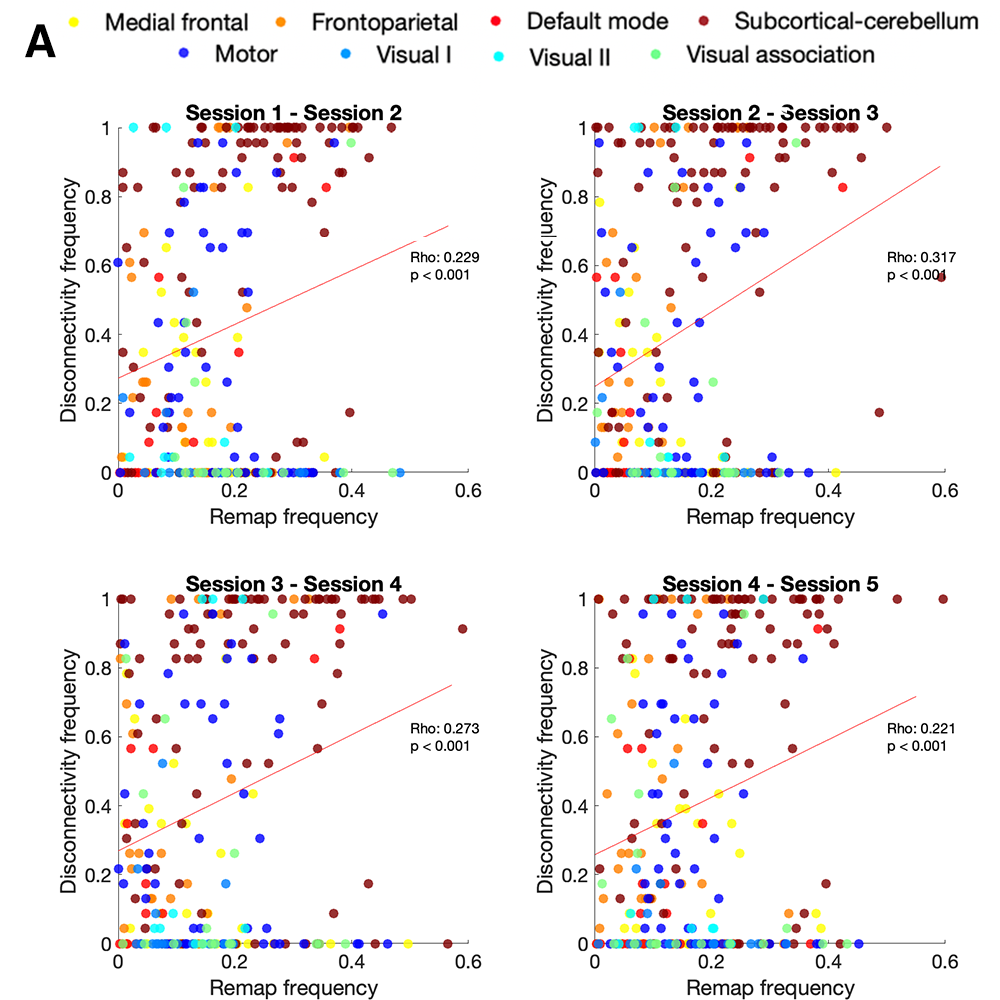
\includegraphics[width=1.0\textwidth]{chapter1/SupplementaryFigure5A.png}
    \caption[]{}
\end{figure}
\null
\vfill
\clearpage
\null
\vfill
\begin{figure}[h!]
		\ContinuedFloat
		\captionsetup{labelformat=adja-page}
    \centering
    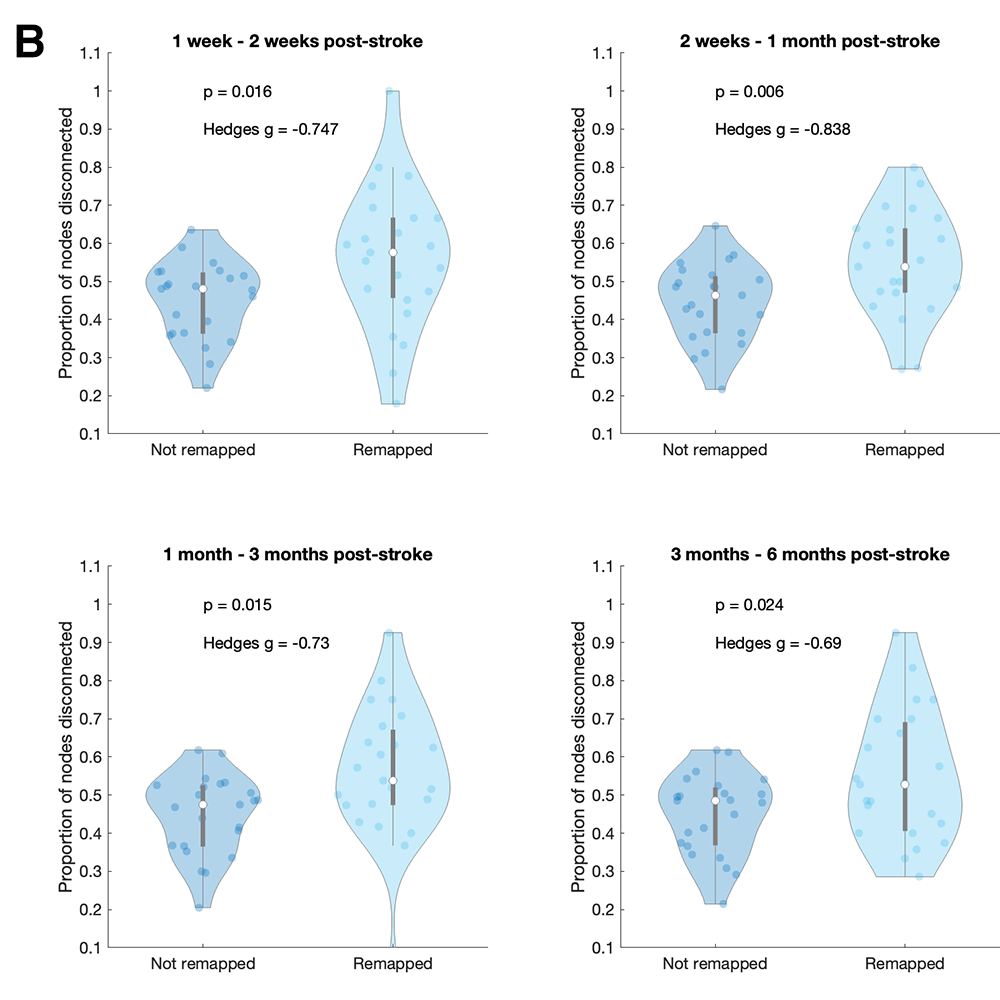
\includegraphics[width=\textwidth]{chapter1/SupplementaryFigure5B.png}
    \caption[]{}
\end{figure}
\null
\vfill
\clearpage




\clearpage
\null
\vfill
\begin{figure}[h!]

    \centering
    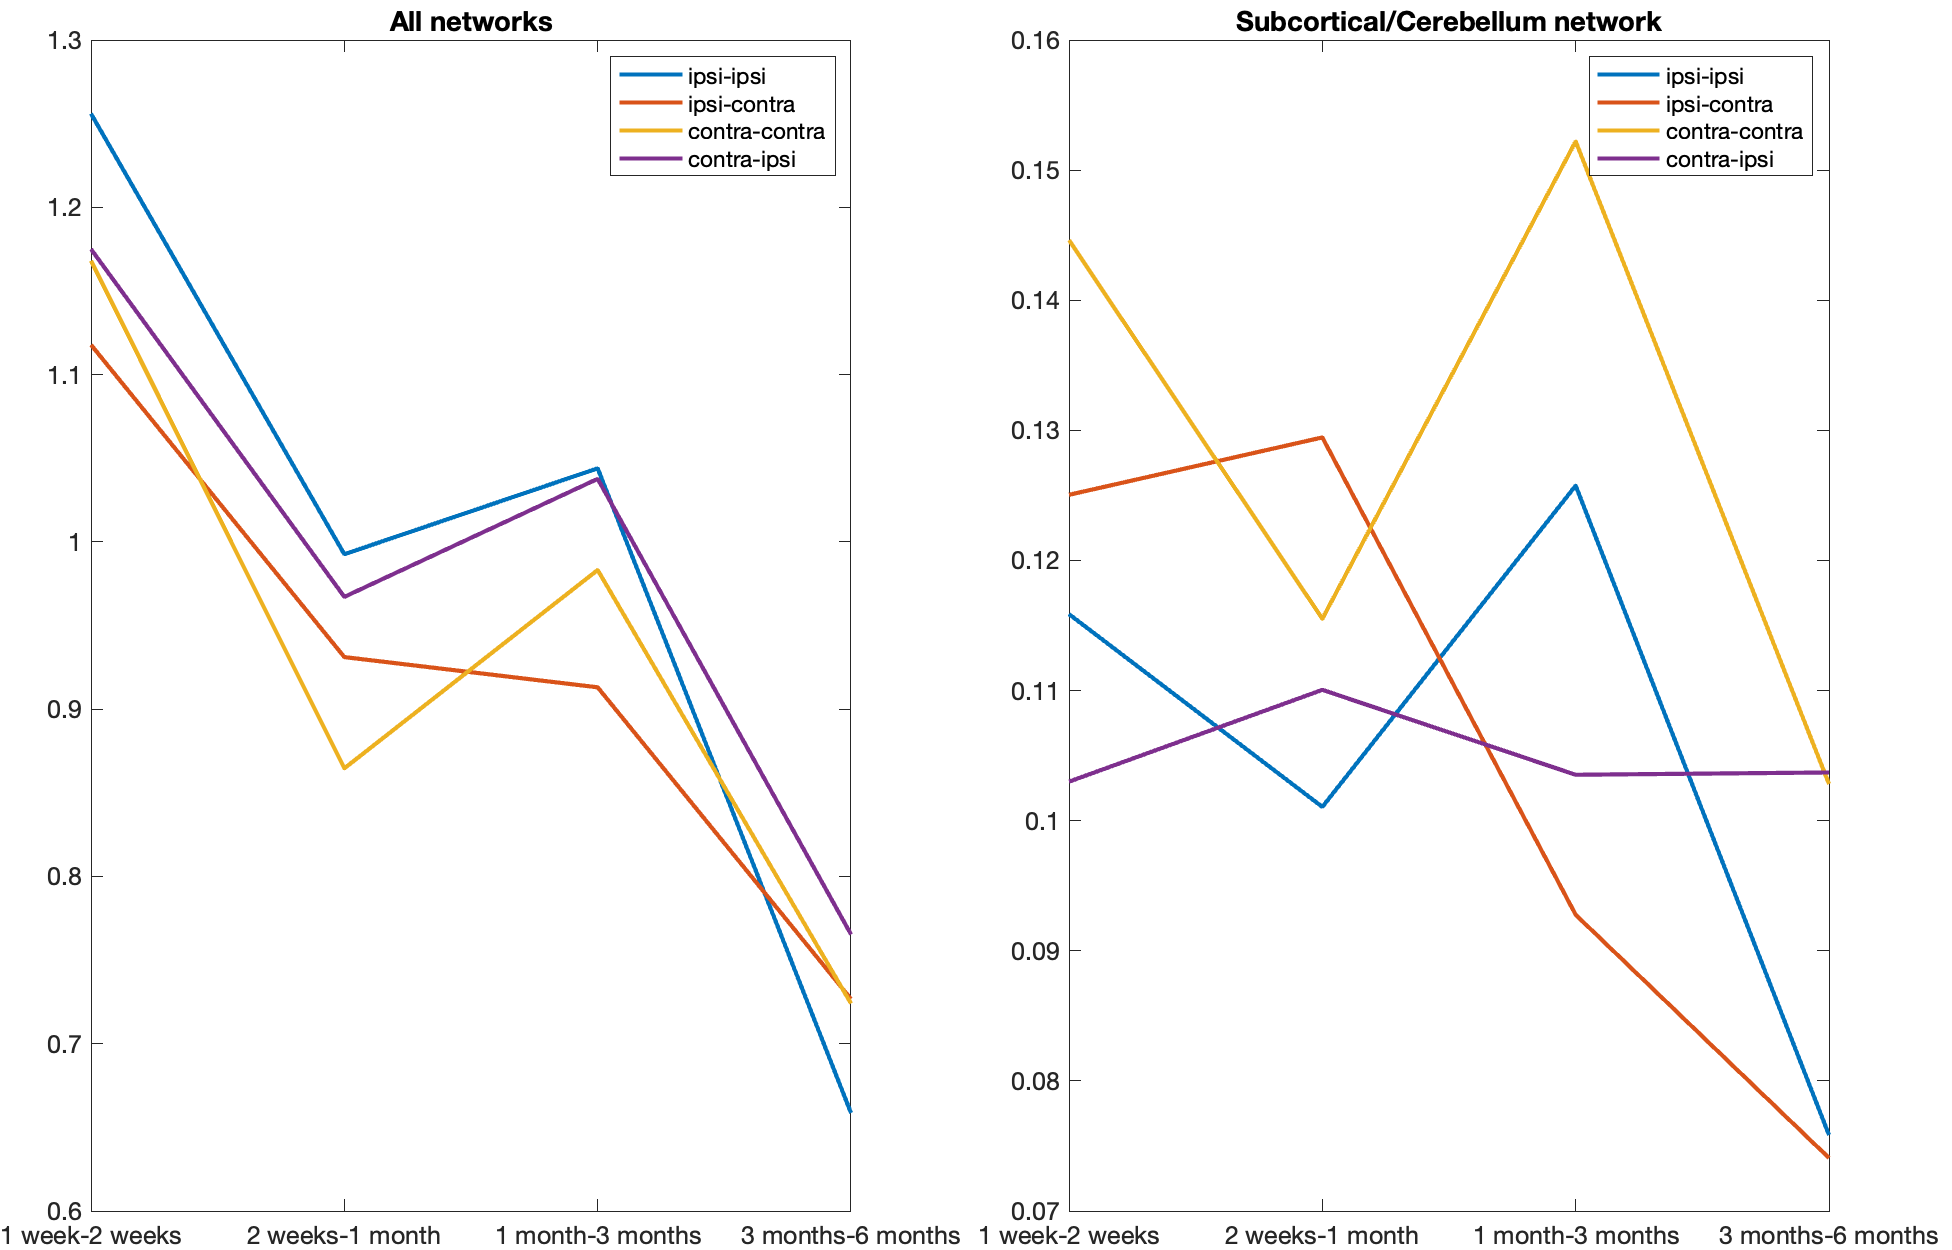
\includegraphics[width=\textwidth]{chapter1/SupplementaryFigure6.png}
       \caption{Number of remaps in}
  \caption*{Left: Number of remaps over 4 time point intervals split into whether the source and target network were in the contralesional or ipsilesional hemisphere. Left: number of remaps organized by hemisphere in only the subcortical/cerebellum network.}
      \label{SupplementaryFigure6}
\end{figure}
\null
\vfill

\clearpage
\null
\vfill
\begin{figure}[!hp]
       \caption{Remapping preferentially occurs in nodes with greater structural connectivity disruption.}
  \caption*{\textbf{A.} Correlations between median ChaCo scores and node remap frequencies across all 23 stroke subjects. Nodes are colored by network assignment. \textbf{B.} ChaCo scores of nodes that remap are significantly greater than ChaCo scores of nodes that do not remap.}
    \label{SupplementaryFigure7}
\end{figure}
\null
\vfill
\clearpage
\null
\vfill
\begin{figure}[h!]
		\ContinuedFloat
		\captionsetup{labelformat=adja-page}
    \centering
    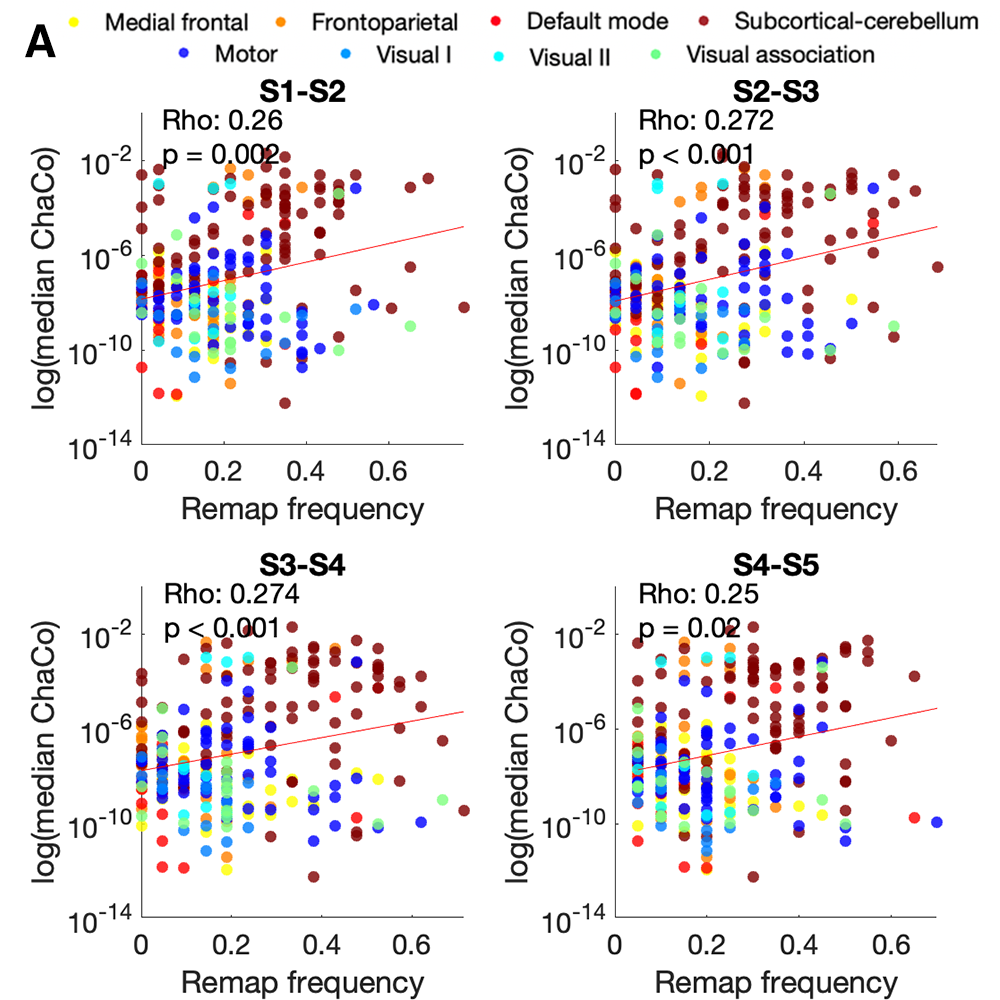
\includegraphics[width=1.0\textwidth]{chapter1/SupplementaryFigure7A.png}
    \caption[]{}
\end{figure}
\null
\vfill
\clearpage
\null
\vfill
\begin{figure}[h!]
		\ContinuedFloat
		\captionsetup{labelformat=adja-page}
    \centering
    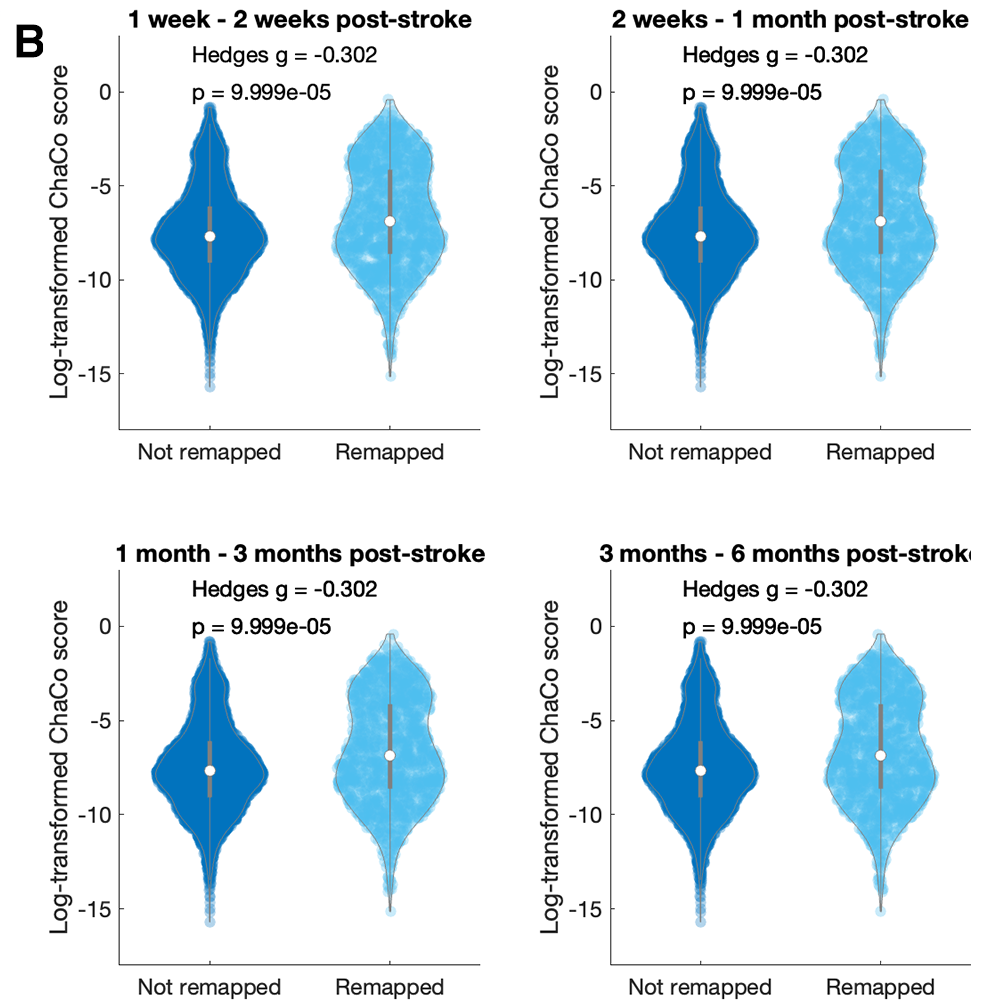
\includegraphics[width=\textwidth]{chapter1/SupplementaryFigure7B.png}
    \caption[]{}
\end{figure}
\null
\vfill
\clearpage



\clearpage
\null
\vfill
\begin{figure}[h!]

    \centering
    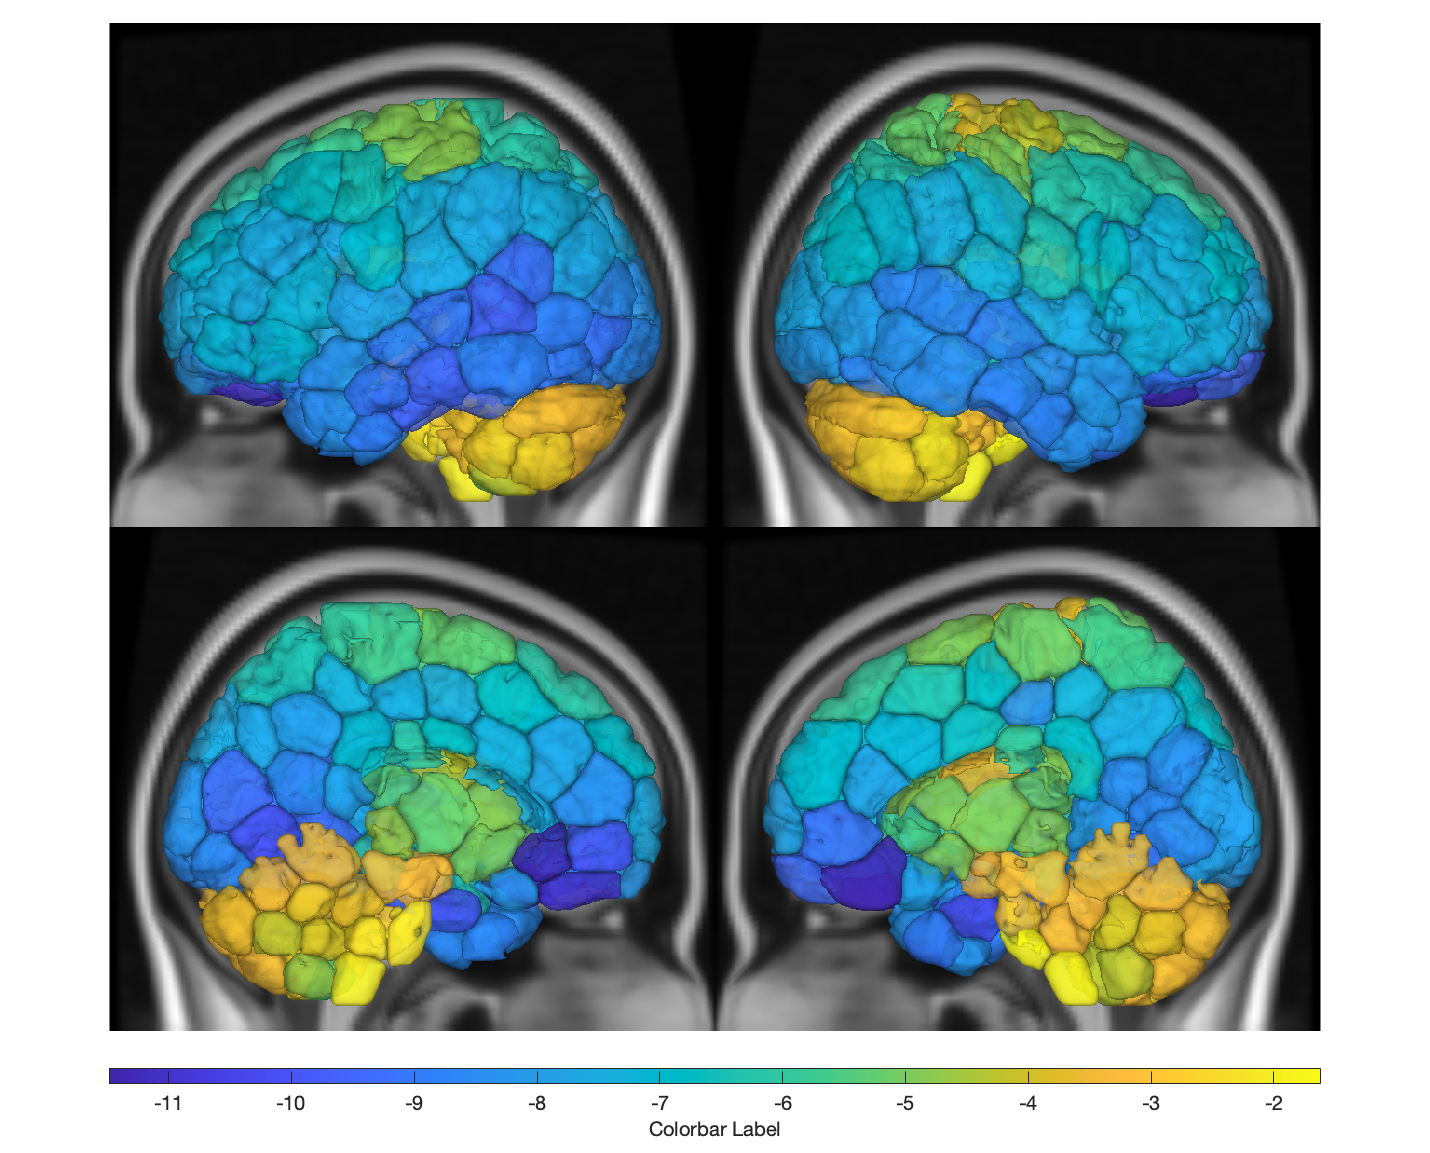
\includegraphics[width=\textwidth]{chapter1/SupplementaryFigure8.png}
       \caption{Group median log-transformed ChaCo scores}
  \caption*{Top row represents lateral view of all ROIs, bottom row represents medial view of all ROIs.}
      \label{SupplementaryFigure8}
\end{figure}
\null
\vfill


\clearpage
\null
\vfill
\begin{figure}[!hp]
       \caption{Correlations between node remapping frequency and t-statistic of node strength.}
  \caption*{For each time point comparison(rows), the node remapping frequency is correlated separately with the 1st and 2nd scan of that time point interval (left/right). The results are very similar.}
    \label{SupplementaryFigure9}
\end{figure}
\null
\vfill
\clearpage
\null
\vfill
\begin{figure}[h!]
		\ContinuedFloat
		\captionsetup{labelformat=adja-page}
    \centering
    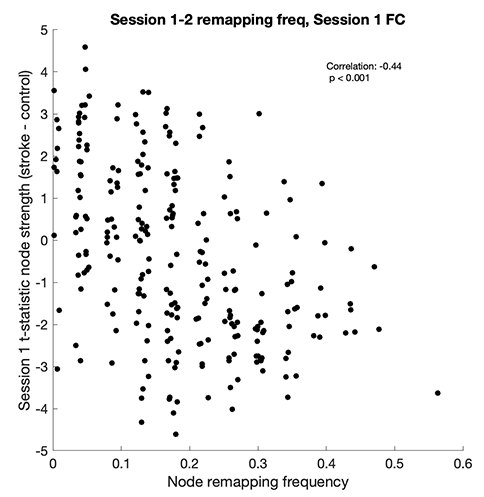
\includegraphics[width=1\textwidth]{chapter1/SupplementaryFigure9A.png}
    \caption[]{}
\end{figure}
\null
\vfill
\clearpage
\null
\vfill
\begin{figure}[h!]
		\ContinuedFloat
		\captionsetup{labelformat=adja-page}
    \centering
    \includegraphics[width=\textwidth]{chapter1/SupplementaryFigure9B.png}
    \caption[]{}
\end{figure}
\null
\vfill
\clearpage
\null
\vfill
\begin{figure}[h!]
		\ContinuedFloat
		\captionsetup{labelformat=adja-page}
    \centering
    \includegraphics[width=\textwidth]{chapter1/SupplementaryFigure9C.png}
    \caption[]{}
\end{figure}
\null
\vfill
\clearpage
\null
\vfill
\begin{figure}[h!]
		\ContinuedFloat
		\captionsetup{labelformat=adja-page}
    \centering
    \includegraphics[width=\textwidth]{chapter1/SupplementaryFigure9D.png}
    \caption[]{}
\end{figure}
\null
\vfill
\clearpage
\null
\vfill
\begin{figure}[h!]
		\ContinuedFloat
		\captionsetup{labelformat=adja-page}
    \centering
    \includegraphics[width=\textwidth]{chapter1/SupplementaryFigure9E.png}
    \caption[]{}
\end{figure}
\null
\vfill
\clearpage
\null
\vfill
\begin{figure}[h!]
		\ContinuedFloat
		\captionsetup{labelformat=adja-page}
    \centering
    \includegraphics[width=\textwidth]{chapter1/SupplementaryFigure9F.png}
    \caption[]{}
\end{figure}
\null
\vfill
\clearpage
\null
\vfill
\begin{figure}[h!]
		\ContinuedFloat
		\captionsetup{labelformat=adja-page}
    \centering
    \includegraphics[width=\textwidth]{chapter1/SupplementaryFigure9G.png}
    \caption[]{}
\end{figure}
\null
\vfill
\clearpage
\null
\vfill
\begin{figure}[h!]
		\ContinuedFloat
		\captionsetup{labelformat=adja-page}
    \centering
    \includegraphics[width=\textwidth]{chapter1/SupplementaryFigure9H.png}
    \caption[]{}
\end{figure}
\null
\vfill

\clearpage
\null
\vfill
\begin{figure}[h!]

    \centering       \caption{Relationships between FC disruption (t-statistic of node strength), SC disruption (ChaCo scores), and remapping over the 2 week - 1 month time interval post-stroke. }
  \caption*{\textbf{A.} Correlation between node remapping frequency and t-statistic of node strength. \textbf{B.} Correlation between node remapping frequency and ChaCo scores. \textbf{C.} Correlation between t-statistic of node strength and ChaCo scores. Dashed horizontal line at y = -6 represents the cut off point of log(ChaCo) -6, representing more SC disruption shown in \textbf{D}, below -6 representing minimal SC disruption is shown in \textbf{E}.  Nodes are colored by network assignment (legend on top).}
      \label{SupplementaryFigure10}
\end{figure}
\null
\vfill
\clearpage
\null
\vfill
\begin{figure}[h!]
		\ContinuedFloat
		\captionsetup{labelformat=adja-page}
    \centering
    \includegraphics[width=1\textwidth]{chapter1/SupplementaryFigure10A.png}
    \caption[]{}
\end{figure}
\null
\vfill
\clearpage
\null
\vfill
\begin{figure}[h!]
		\ContinuedFloat
		\captionsetup{labelformat=adja-page}
    \centering
    \includegraphics[width=\textwidth]{chapter1/SupplementaryFigure10B.png}
    \caption[]{}
\end{figure}
\null
\vfill
\clearpage
\null
\vfill
\begin{figure}[h!]
		\ContinuedFloat
		\captionsetup{labelformat=adja-page}
    \centering
    \includegraphics[width=\textwidth]{chapter1/SupplementaryFigure10C.png}
    \caption[]{}
\end{figure}
\null
\vfill
\clearpage
\null
\vfill
\begin{figure}[h!]
		\ContinuedFloat
		\captionsetup{labelformat=adja-page}
    \centering
    \includegraphics[width=\textwidth]{chapter1/SupplementaryFigure10DE.png}
    \caption[]{}
\end{figure}
\null
\vfill
\clearpage
\null
\vfill


\begin{figure}[h!]

    \centering       \caption{Relationships between FC disruption (t-statistic of node strength), SC disruption (ChaCo scores), and remapping over the 1 month - 3 month time interval post-stroke. }
  \caption*{\textbf{A.} Correlation between node remapping frequency and t-statistic of node strength. \textbf{B.} Correlation between node remapping frequency and ChaCo scores. \textbf{C.} Correlation between t-statistic of node strength and ChaCo scores. Dashed horizontal line at y = -6 represents the cut off point of log(ChaCo) -6, representing more SC disruption shown in \textbf{D}, below -6 representing minimal SC disruption is shown in \textbf{E}.  Nodes are colored by network assignment (legend on top).}
      \label{SupplementaryFigure11}
\end{figure}
\null
\vfill
\clearpage
\null
\vfill
\begin{figure}[h!]
		\ContinuedFloat
		\captionsetup{labelformat=adja-page}
    \centering
    \includegraphics[width=1\textwidth]{chapter1/SupplementaryFigure11A.png}
    \caption[]{}
\end{figure}
\null
\vfill
\clearpage
\null
\vfill
\begin{figure}[h!]
		\ContinuedFloat
		\captionsetup{labelformat=adja-page}
    \centering
    \includegraphics[width=\textwidth]{chapter1/SupplementaryFigure11B.png}
    \caption[]{}
\end{figure}
\null
\vfill
\clearpage
\null
\vfill
\begin{figure}[h!]
		\ContinuedFloat
		\captionsetup{labelformat=adja-page}
    \centering
    \includegraphics[width=\textwidth]{chapter1/SupplementaryFigure11C.png}
    \caption[]{}
\end{figure}
\null
\vfill
\clearpage
\null
\vfill
\begin{figure}[h!]
		\ContinuedFloat
		\captionsetup{labelformat=adja-page}
    \centering
    \includegraphics[width=\textwidth]{chapter1/SupplementaryFigure11DE.png}
    \caption[]{}
\end{figure}
\null
\vfill
\clearpage
\null
\vfill



\begin{figure}[h!]

    \centering       \caption{Relationships between FC disruption (t-statistic of node strength), SC disruption (ChaCo scores), and remapping over the 3 month - 6 month time interval post-stroke. }
  \caption*{\textbf{A.} Correlation between node remapping frequency and t-statistic of node strength. \textbf{B.} Correlation between node remapping frequency and ChaCo scores. \textbf{C.} Correlation between t-statistic of node strength and ChaCo scores. Dashed horizontal line at y = -6 represents the cut off point of log(ChaCo) -6, representing more SC disruption shown in \textbf{D}, below -6 representing minimal SC disruption is shown in \textbf{E}.  Nodes are colored by network assignment (legend on top).}
      \label{SupplementaryFigure12}
\end{figure}
\null
\vfill
\clearpage
\null
\vfill
\begin{figure}[h!]
		\ContinuedFloat
		\captionsetup{labelformat=adja-page}
    \centering
    \includegraphics[width=1\textwidth]{chapter1/SupplementaryFigure12A.png}
    \caption[]{}
\end{figure}
\null
\vfill
\clearpage
\null
\vfill
\begin{figure}[h!]
		\ContinuedFloat
		\captionsetup{labelformat=adja-page}
    \centering
    \includegraphics[width=\textwidth]{chapter1/SupplementaryFigure12B.png}
    \caption[]{}
\end{figure}
\null
\vfill
\clearpage
\null
\vfill
\begin{figure}[h!]
		\ContinuedFloat
		\captionsetup{labelformat=adja-page}
    \centering
    \includegraphics[width=\textwidth]{chapter1/SupplementaryFigure12C.png}
    \caption[]{}
\end{figure}
\null
\vfill
\clearpage
\null
\vfill
\begin{figure}[h!]
		\ContinuedFloat
		\captionsetup{labelformat=adja-page}
    \centering
    \includegraphics[width=\textwidth]{chapter1/SupplementaryFigure12DE.png}
    \caption[]{}
\end{figure}
\null
\vfill
\clearpage
\null
\vfill



\begin{figure}[h!]

    \centering       \caption{Node-level remapping frequencies, calculated using FC matrices derived from Pearson correlation with threshold of 1 control subject to determine significant remaps}
  \caption*{\textbf{A.} Node remap frequencies $> 0.1$ averaged across 4 time point comparisons are plotted on a glass brain. Inset figures display a lateral view (top row) and medial view (bottom row). \textbf{B.} Node remap frequencies above 0.1 are plotted on a glass brain, displayed separately for each time point comparison. \textbf{C.} Network-level sum of remaps, averaged across all 4 comparisons, and normalized by the number of regions in each network. Remaps are separated based on their position relative to the lesion (contralesional vs. ipsilesional). \textbf{D.} Network-level sum of remaps, displayed separately for each time point comparisons, normalized by the number of regions in each network. Ipsilesional = in the same hemisphere as the lesion, contralesional = in the opposite hemisphere as the lesion.}
      \label{SupplementaryFigure13}
\end{figure}
\null
\vfill
\clearpage
\null
\vfill
\begin{figure}[h!]
		\ContinuedFloat
		\captionsetup{labelformat=adja-page}
    \centering
    \includegraphics[width=1\textwidth]{chapter1/SupplementaryFigure13A.png}
    \caption[]{}
\end{figure}
\null
\vfill
\clearpage
\null
\vfill
\begin{figure}[h!]
		\ContinuedFloat
		\captionsetup{labelformat=adja-page}
    \centering
    \includegraphics[width=\textwidth]{chapter1/SupplementaryFigure13B.png}
    \caption[]{}
\end{figure}
\null
\vfill
\clearpage
\null
\vfill
\begin{figure}[h!]
		\ContinuedFloat
		\captionsetup{labelformat=adja-page}
    \centering
    \includegraphics[width=\textwidth]{chapter1/SupplementaryFigure13C.png}
    \caption[]{}
\end{figure}
\null
\vfill
\clearpage
\null
\vfill
\begin{figure}[h!]
		\ContinuedFloat
		\captionsetup{labelformat=adja-page}
    \centering
    \includegraphics[width=\textwidth]{chapter1/SupplementaryFigure13D.png}
    \caption[]{}
\end{figure}
\null
\vfill
\clearpage
\null
\vfill

\begin{figure}[h!]

    \centering       \caption{Relationship between ChaCo scores and remapping calculated using FC matrices derived from Pearson correlations with a threshold of 1 control subject}
  \caption*{ \textbf{A.} Correlations between average ChaCo scores and regional remap frequencies across all 23 stroke subjects. Regions are colored by network assignment. \textbf{B.} ChaCo scores of regions that remap are significantly greater than ChaCo scores of regions that do not remap.}
      \label{SupplementaryFigure14}
\end{figure}
\null
\vfill
\clearpage
\null
\vfill
\begin{figure}[h!]
		\ContinuedFloat
		\captionsetup{labelformat=adja-page}
    \centering
    \includegraphics[width=1\textwidth]{chapter1/SupplementaryFigure14A.png}
    \caption[]{}
\end{figure}
\null
\vfill
\clearpage
\null
\vfill
\begin{figure}[h!]
		\ContinuedFloat
		\captionsetup{labelformat=adja-page}
    \centering
    \includegraphics[width=\textwidth]{chapter1/SupplementaryFigure14B.png}
    \caption[]{}
\end{figure}
\null
\vfill
\clearpage
\null
\vfill

\begin{figure}[h!]

    \centering       \caption{Relationship between motor recovery and amount of remapping, calculated using FC matrices derived from Pearson correlations, with threshold of 1 control subject }
  \caption*{ \textbf{A.} Correlations between average ChaCo scores and regional remap frequencies across all 23 stroke subjects. Regions are colored by network assignment. \textbf{B.} ChaCo scores of regions that remap are significantly greater than ChaCo scores of regions that do not remap.}
      \label{SupplementaryFigure15}
\end{figure}
\null
\vfill
\clearpage
\null
\vfill
\begin{figure}[h!]
		\ContinuedFloat
		\captionsetup{labelformat=adja-page}
    \centering
    \includegraphics[width=1\textwidth]{chapter1/SupplementaryFigure15AB.png}
    \caption[]{}
\end{figure}
\null
\vfill
\clearpage
\null
\vfill
\begin{figure}[h!]
		\ContinuedFloat
		\captionsetup{labelformat=adja-page}
    \centering
    \includegraphics[width=\textwidth]{chapter1/SupplementaryFigure15C.png}
    \caption[]{}
\end{figure}
\null
\vfill
\clearpage
\null
\vfill

\begin{figure}[h!]
		\ContinuedFloat
		\captionsetup{labelformat=adja-page}
    \centering
    \includegraphics[width=\textwidth]{chapter1/SupplementaryFigure15D.png}
    \caption[]{}
\end{figure}
\null
\vfill
\clearpage
\null
\vfill
\begin{figure}[h!]

    \centering       \caption{Node-level remapping frequencies, with remapping calculated using a cutoff of 1 control subject to define significant remaps }
  \caption*{ \textbf{A.} Node remap frequencies above 0.1, for clarity, are plotted on a glass brain, averaged across 4 time point comparisons.  Inset figures display a lateral view (top row) and medial view (bottom row). \textbf{B.} Node remap frequencies plotted on a glass brain, displayed separately for each time point comparison. \textbf{C.} Network-level sum of remaps, averaged across all 4 comparisons, and normalized by the number of regions in each network. Remaps are separated based on their position relative to the lesion (contralesional vs. ipsilesional). \textbf{D.} Network-level sum of remaps, displayed separately for each time point comparisons, normalized by the number of regions in each network. Ipsilesional = in the same hemisphere as the lesion, contralesional = in the opposite hemisphere as the lesion.}
      \label{SupplementaryFigure16}
\end{figure}
\null
\vfill
\clearpage
\null
\vfill
\begin{figure}[h!]
		\ContinuedFloat
		\captionsetup{labelformat=adja-page}
    \centering
    \includegraphics[width=1\textwidth]{chapter1/SupplementaryFigure16A.png}
    \caption[]{}
\end{figure}
\null
\vfill
\clearpage
\null
\vfill
\begin{figure}[h!]
		\ContinuedFloat
		\captionsetup{labelformat=adja-page}
    \centering
    \includegraphics[width=\textwidth]{chapter1/SupplementaryFigure16B.png}
    \caption[]{}
\end{figure}
\null
\vfill
\clearpage
\null
\vfill

\begin{figure}[h!]
		\ContinuedFloat
		\captionsetup{labelformat=adja-page}
    \centering
    \includegraphics[width=\textwidth]{chapter1/SupplementaryFigure16C.png}
    \caption[]{}
\end{figure}
\null
\vfill
\clearpage
\null
\vfill
\begin{figure}[h!]
		\ContinuedFloat
		\captionsetup{labelformat=adja-page}
    \centering
    \includegraphics[width=\textwidth]{chapter1/SupplementaryFigure16D.png}
    \caption[]{}
\end{figure}
\null
\vfill
\clearpage
\null
\vfill


\begin{figure}[h!]

    \centering       \caption{Relationship between ChaCo scores and remapping calculated using a cutoff of 1 control subject}
  \caption*{ \textbf{A.} Correlations between average ChaCo scores and regional remap frequencies across all 23 stroke subjects. Regions are colored by network assignment. \textbf{B.} ChaCo scores of regions that remap are significantly greater than ChaCo scores of regions that do not remap.}
      \label{SupplementaryFigure17}
\end{figure}
\null
\vfill
\clearpage
\null
\vfill
\begin{figure}[h!]
		\ContinuedFloat
		\captionsetup{labelformat=adja-page}
    \centering
    \includegraphics[width=1\textwidth]{chapter1/SupplementaryFigure17A.png}
    \caption[]{}
\end{figure}
\null
\vfill
\clearpage
\null
\vfill
\begin{figure}[h!]
		\ContinuedFloat
		\captionsetup{labelformat=adja-page}
    \centering
    \includegraphics[width=\textwidth]{chapter1/SupplementaryFigure17B.png}
    \caption[]{}
\end{figure}
\null
\vfill
\clearpage
\null
\vfill


\begin{figure}[h!]

    \centering       \caption{Relationship between motor recovery and amount of remapping, with remapping calculated using a cutoff of 1 control subject to define significant remaps}
  \caption*{ \textbf{A.} Pearson correlation between individuals' total number of early remaps (between 1 week FC and 2 week FC) and their change in Fugl-Meyer scores between 1 week and 6 months post-stroke. \textbf{B.} Pearson correlation between individuals' total number of early remaps (between 1 week FC and 2 week FC) and 1 week Fugl-Meyer scores, controlling for scan lengths at 1 week post-stroke at 2 weeks post stroke. \textbf{C.} Results from linear mixed effects analysis; each color indicates a different individuals' longitudinal time point. \textbf{D.} Pearson correlation between the total remaps observed between each pair of time points and the change in Fugl-Meyer scores between time points, controlling for the scan length of the 2 scans involved in the remapping calculation.}
      \label{SupplementaryFigure18}
\end{figure}
\null
\vfill
\clearpage
\null
\vfill
\begin{figure}[h!]
		\ContinuedFloat
		\captionsetup{labelformat=adja-page}
    \centering
    \includegraphics[width=1\textwidth]{chapter1/SupplementaryFigure18AB.png}
    \caption[]{}
\end{figure}
\null
\vfill
\clearpage
\null
\vfill
\begin{figure}[h!]
		\ContinuedFloat
		\captionsetup{labelformat=adja-page}
    \centering
    \includegraphics[width=\textwidth]{chapter1/SupplementaryFigure18C.png}
    \caption[]{}
\end{figure}
\null
\vfill
\clearpage
\null
\vfill

\begin{figure}[h!]
		\ContinuedFloat
		\captionsetup{labelformat=adja-page}
    \centering
    \includegraphics[width=\textwidth]{chapter1/SupplementaryFigure18D.png}
    \caption[]{}
\end{figure}
\null
\vfill
\clearpage
\null
\vfill


\begin{figure}[h!]

    \centering
    \includegraphics[width=\textwidth]{chapter1/SupplementaryFigure19.png}
       \caption{Average overlap between each gray matter regions and lesions}
  \caption*{Calculated for each subject as the total volume of the lesion inside each region divided by the total region volume. Displaying only regions with an average overlap with the lesion above zero.}
      \label{SupplementaryFigure19}
\end{figure}
\null
\vfill

\begin{figure}[h!]

    \centering
    \includegraphics[width=\textwidth]{chapter1/SupplementaryFigure20.png}
       \caption{Correlation between framewise displacement between scans and number of remaps.}
  \caption*{}
      \label{SupplementaryFigure20}
\end{figure}
\null
\vfill


\chapter{Supplementary material for Chapter 2}
\label{chap:5}


\begin{table}[h]
\begin{tabular}{ |c| c| c| c| }

\hline
ID	& Lesion Location &	Handedness & Dominant CST damage \\
			
\hline 
SUB1	& Right Pons &	R &	Non-dominant CST \\
SUB2	& Right Pons &	R &	Non-dominant CST \\
SUB3	& Left Pons &	R &	Dominant CST \\
SUB4	& Left Pons	 & R &	Dominant CST \\
SUB5	& Right Pons &	R &	Non-dominant CST \\
SUB6 & 	Left Pons and midbrain*	 & L &	Dominant CST \\
SUB7 & 	Right Pons &	L &	Dominant CST \\
SUB8 & 	Right Pons &	R &	Non-dominant CST \\
SUB9 & 	Right Pons &	R &	Non-dominant CST \\
SUB10 & 	Right Pons	 & R &	Non-dominant CST \\
SUB11 &	Left Pons & 	R &	Dominant CST \\
SUB12 &	Left bulbus medullae &	B &	Dominant CST \\
SUB13 &	Left bulbus medullae &	R &	Dominant CST \\
SUB14 &	Right bulbus medullae &	R &	Non-dominant CST \\
SUB15 &	Right Pons and cerebellum &	R &	Non-dominant CST \\
SUB16 &	Left Pons &	R &	Dominant CST \\
SUB17 &	Left Pons &	R	 & Dominant CST \\
SUB18 &	Right Pons &	R &	Non-dominant CST \\
SUB19  &	Right Pons &	R	 & Non-dominant CST \\
SUB20 &	Right Pons &	R &	Non-dominant CST \\
SUB21 &	Right Pons &	R &	Non-dominant CST \\
SUB22 &	Left Pons &	R &	Dominant CST \\
SUB23 &	Right Pons &	R &	Non-dominant CST \\
\hline
\end{tabular}
\caption{
* Overlap with L and R CST tracts. Breakdown of subjects according to lesion side, handedness, and dominant-hemisphere CST damage. Blue subjects indicate those that were included in the linear model as having "Dominant CST damage" assessing the effect of CST damage on FPN+ recruitment in recovery. Note that SUB12 has damage to their dominant CST but does not have motor scores for the chronic period, and was not included in the model. L;left, R; right, B; both}
\end{table}

\null
\vfill
\clearpage
\null
\vfill

\begin{figure}[h!]

    \centering       \caption{Lesion and motor scores for pontine stroke subjects. }
  \caption*{ \textbf{a}. Distribution of lesions on MNI template. \textbf{b}. Fugl-Meyer scores across time points (normalized 0-100).}
      \label{2_SupplementaryFigure1}
\end{figure}
\null
\vfill
\clearpage
\null
\vfill
\begin{figure}[h!]
		\ContinuedFloat
		\captionsetup{labelformat=adja-page}
    \centering
    \includegraphics[width=1\textwidth]{chapter2/SupplementaryFig1a.png}
    \caption[]{}
\end{figure}
\null
\vfill
\clearpage
\null
\vfill
\begin{figure}[h!]
		\ContinuedFloat
		\captionsetup{labelformat=adja-page}
    \centering
    \includegraphics[width=\textwidth]{chapter2/SupplementaryFig1b.png}
    \caption[]{}
\end{figure}
\null
\vfill
\clearpage
\null
\vfill


\begin{figure}[h!]

    \centering
    \includegraphics[width=\textwidth]{chapter2/SupplementaryFig2.png}
       \caption{Right hemisphere lesion location relative to brainstem corticospinal tracts. }
  \caption*{Red = lesion. Blue = right CST, yellow = left CST. Four views of the lesions/CSTs are displayed, from left to right: left lateral view, anterior view, right lateral view. A "D" above the subject identifiers ("SX") indicates that the lesion is in that subject's dominant hemisphere. Numbers below subject identifiers indicate Dice overlap between lesion and ipsilesional CST. }
      \label{2_SupplementaryFigure2}
\end{figure}
\null
\vfill
\clearpage
\null
\vfill


\begin{figure}[h!]

    \centering
    \includegraphics[width=\textwidth]{chapter2/SupplementaryFig3.png}
       \caption{Left hemisphere lesion location relative to brainstem corticospinal tracts. }
  \caption*{Red = lesion. Blue = right CST, yellow = left CST. Four views of the lesions/CSTs are displayed, from left to right: left lateral view, anterior view, right lateral view. A "D" above the subject identifiers ("SX") indicates that the lesion is in that subject's dominant hemisphere. Numbers below subject identifiers indicate Dice overlap between lesion and ipsilesional CST. }
      \label{2_SupplementaryFigure3}
\end{figure}
\null
\vfill
\clearpage
\null






% Supplementary Figure 4 = A.1




% Supplementary FIgure 5  = incoming


\vfill
\begin{figure}[h!]
    \centering       \caption{Centroids derived from clustering stroke and control subjects separately. }
  \caption*{ Bottom left: Hypothesized mapping from the centroids derived from clustering both groups together to the individually clustered centroids. Bottom right: Correlation of the centroids derived from separately clustering control and stroke groups.}
      \label{2_SupplementaryFigure6}
\end{figure}
\null
\vfill
\clearpage

\null
\vfill
\begin{figure}[h!]
		\ContinuedFloat
		\captionsetup{labelformat=adja-page}
    \centering
    \includegraphics[width=1\textwidth]{chapter2/SupplementaryFig6a.png}
    \caption[]{}
\end{figure}
\null
\vfill
\clearpage
\null
\vfill
\begin{figure}[h!]
		\ContinuedFloat
		\captionsetup{labelformat=adja-page}
    \centering
    \includegraphics[width=\textwidth]{chapter2/SupplementaryFig6b.png}
    \caption[]{}
\end{figure}
\null
\vfill
\clearpage
\null
\vfill


\begin{figure}[h!]
    \centering       \caption{Centroids derived from clustering fMRI data parcellated using different atlases}
  \caption*{ \textbf{top:} FreeSurfer-86 region (group-average; not individual anatomical parcellations) and \textbf{bottom:} CC400 . Note that the regions are parcellated into 9  networks here, instead of 8, and there are missing (VIS II, VIS III, MED FRONT) and additional (ATTN-VEN, ATTN-DORS, LIMB) networks that are not in the shen268 network parcellation. SUB + CEREB are also combined in the shen268 parcellation, and the label SOM is used here instead of MOTOR in the main results.}
      \label{2_SupplementaryFigure7}
\end{figure}
\null
\vfill
\clearpage

\null
\vfill
\begin{figure}[h!]
		\ContinuedFloat
		\captionsetup{labelformat=adja-page}
    \centering
    \includegraphics[width=1\textwidth]{chapter2/SupplementaryFig7a.png}
    \caption[]{}
\end{figure}
\null
\vfill
\clearpage
\null
\vfill
\begin{figure}[h!]
		\ContinuedFloat
		\captionsetup{labelformat=adja-page}
    \centering
    \includegraphics[width=\textwidth]{chapter2/SupplementaryFig7b.png}
    \caption[]{}
\end{figure}
\null
\vfill
\clearpage
\null
\vfill



\begin{figure}[h!]
    \centering       \caption{Full session-specific group differences in brain dynamics parameters.}
  \caption*{ Group differences in fractional occupancy (top row), dwell time (middle row), and appearance rate (bottom row) with k = 4. Aside from the group differences reported in the main paper in $FPN^+$, there are group differences in $AR^{MOTOR^+}_{6mo}$.  Boxplot whiskers indicate the 25th and 75th percentiles, and the central mark indicates the median.}
      \label{2_SupplementaryFigure8}
\end{figure}
\null
\vfill
\clearpage
\null
\vfill
\begin{figure}[h!]
		\ContinuedFloat
		\captionsetup{labelformat=adja-page}
    \centering
    \includegraphics[width=0.5\textwidth]{chapter2/SupplementaryFig8a.png}
    \caption[]{}
\end{figure}
\null
\vfill
\clearpage
\null
\vfill
\begin{figure}[h!]
		\ContinuedFloat
		\captionsetup{labelformat=adja-page}
    \centering
    \includegraphics[width=0.5\textwidth]{chapter2/SupplementaryFig8b.png}
    \caption[]{}
\end{figure}
\null
\vfill
\clearpage
\null
\vfill
\begin{figure}[h!]
		\ContinuedFloat
		\captionsetup{labelformat=adja-page}
    \centering
    \includegraphics[width=0.5\textwidth]{chapter2/SupplementaryFig8c.png}
    \caption[]{}
\end{figure}
\null
\vfill
\clearpage
\null
\vfill
\begin{figure}[h!]
		\ContinuedFloat
		\captionsetup{labelformat=adja-page}
    \centering
    \includegraphics[width=0.5\textwidth]{chapter2/SupplementaryFig8d.png}
    \caption[]{}
\end{figure}
\null
\vfill
\clearpage
\null
\vfill



\begin{figure}[h!]
    \centering       \caption{Correlation between brain state parameters and age in control and stroke subjects. }
  \caption*{Colors indicate Pearson's correlation coefficient, text represents Benjamini-Hochberg corrected p-values (alpha = 0.05). \textbf{a.} Correlation between age and dwell time, fractional occupancy, and appearance rate in control subjects. \textbf{b.} Correlation between age and transition probabilities in control subjects. \textbf{d.} Correlation between age and dwell time, fractional occupancy, and appearance rate in stroke subjects. \textbf{c.} Correlation between age and transition probabilities in stroke subjects.}
      \label{2_SupplementaryFigure9}
\end{figure}
\null
\vfill
\clearpage
\null
\vfill
\begin{figure}[h!]
		\ContinuedFloat
		\captionsetup{labelformat=adja-page}
    \centering
    \includegraphics[width=0.4\textwidth]{chapter2/SupplementaryFig9a.png}
    \caption[]{}
\end{figure}
\null
\vfill
\clearpage
\null
\vfill
\begin{figure}[h!]
		\ContinuedFloat
		\captionsetup{labelformat=adja-page}
    \centering
    \includegraphics[width=1\textwidth]{chapter2/SupplementaryFig9b.png}
    \caption[]{}
\end{figure}
\null
\vfill
\clearpage
\null
\vfill
\begin{figure}[h!]
		\ContinuedFloat
		\captionsetup{labelformat=adja-page}
    \centering
    \includegraphics[width=0.4\textwidth]{chapter2/SupplementaryFig9c.png}
    \caption[]{}
\end{figure}
\null
\vfill
\clearpage
\null
\vfill
\begin{figure}[h!]
		\ContinuedFloat
		\captionsetup{labelformat=adja-page}
    \centering
    \includegraphics[width=1\textwidth]{chapter2/SupplementaryFig9d.png}
    \caption[]{}
\end{figure}
\null
\vfill
\clearpage
\null
\vfill

\begin{figure}[h!]
    \centering       \caption{Visualization of dwell times and fractional occupancies of stroke and control subjects.}
  \caption*{Dwell times and fractional occupancies of stroke subjects (left) and control subjects (right) at session 1.}
      \label{2_SupplementaryFigure10}
\end{figure}
\null
\vfill
\clearpage
\null
\vfill
\begin{figure}[h!]
		\ContinuedFloat
		\captionsetup{labelformat=adja-page}
    \centering
    \includegraphics[width=0.7\textwidth]{chapter2/SupplementaryFig10a.png}
    \caption[]{}
\end{figure}
\null
\vfill
\clearpage
\null
\vfill
\begin{figure}[h!]
		\ContinuedFloat
		\captionsetup{labelformat=adja-page}
    \centering
    \includegraphics[width=0.7\textwidth]{chapter2/SupplementaryFig10b.png}
    \caption[]{}
\end{figure}
\null
\vfill
\clearpage
\null
\vfill
\begin{figure}[h!]
    \centering       \caption{Main results from chapter 2 replicated with k = 5 clusters.}
  \caption*{ \textbf{A}. Cluster centroids from k = 5 show that largely the same states appear ($FPN^+$,$FPN^-$, $MOTOR^+$, $MOTOR^-$) alongside a new state ($VIS^-$) characterized by low amplitude activations of the visual network. \textbf{B}. Stroke-control differences in fractional occupancy (top row), dwell time (middle row), and appearance rate (bottom row) mirror differences observed with k = 4, particularly group differences in FO and DT in $FPN^+$. Notably, $FPN^-$ displays significant group differences in DT using k = 5 but not k = 4. Boxplot whiskers indicate the 25th and 75th percentiles, and the central mark indicates the median. \textbf{C.} Stroke-control differences in transition probabilities between states mirrors results with k = 4, particularly reduced transition probability from $MOTOR^-$ into $FPN^+$ and reduced persistence probability of $FPN^+$. \textbf{D}. Linear model results examining the relationship between longitudinal changes in $DT^{FPN^+}$ and $FO^{FPN^+}$ and motor recovery in subjects with dominant hemisphere CST damage. Trend-level effects are replicated with k = 5 but do not reach statistical significance (p-value of marginal effect of $\Delta DT^{FPN^+}$ = 0.0339 (uncorrected), $\Delta FO^{FPN^+}$ = 0.10640 (uncorrected)). Interaction effects are not replicated.}
      \label{2_SupplementaryFigure11}
\end{figure}
\null
\vfill
\clearpage
\null
\vfill
\begin{figure}[h!]
		\ContinuedFloat
		\captionsetup{labelformat=adja-page}
    \centering
    \includegraphics[width=1\textwidth]{chapter2/SupplementaryFig11a.png}
    \caption[]{}
\end{figure}
\null
\vfill
\clearpage
\null
\vfill
\begin{figure}[h!]
		\ContinuedFloat
		\captionsetup{labelformat=adja-page}
    \centering
    \includegraphics[width=0.35\textwidth]{chapter2/SupplementaryFig11b.png}
    \caption[]{}
\end{figure}
\null
\vfill
\clearpage
\null
\vfill
\begin{figure}[h!]
		\ContinuedFloat
		\captionsetup{labelformat=adja-page}
    \centering
    \includegraphics[width=0.35\textwidth]{chapter2/SupplementaryFig11c.png}
    \caption[]{}
\end{figure}
\null
\vfill
\clearpage
\null
\vfill
\begin{figure}[h!]
		\ContinuedFloat
		\captionsetup{labelformat=adja-page}
    \centering
    \includegraphics[width=0.35\textwidth]{chapter2/SupplementaryFig11d.png}
    \caption[]{}
\end{figure}
\null
\vfill
\clearpage
\null
\vfill
\begin{figure}[h!]
		\ContinuedFloat
		\captionsetup{labelformat=adja-page}
    \centering
    \includegraphics[width=0.35\textwidth]{chapter2/SupplementaryFig11e.png}
    \caption[]{}
\end{figure}
\null
\vfill
\clearpage
\null
\vfill
\begin{figure}[h!]
		\ContinuedFloat
		\captionsetup{labelformat=adja-page}
    \centering
    \includegraphics[width=0.35\textwidth]{chapter2/SupplementaryFig11f.png}
    \caption[]{}
\end{figure}
\null
\vfill
\clearpage
\null
\vfill
\begin{figure}[h!]
		\ContinuedFloat
		\captionsetup{labelformat=adja-page}
    \centering
    \includegraphics[width=1\textwidth]{chapter2/SupplementaryFig11g.png}
    \caption[]{}
\end{figure}
\null
\vfill
\clearpage
\null
\vfill
\begin{figure}[h!]
		\ContinuedFloat
		\captionsetup{labelformat=adja-page}
    \centering
    \includegraphics[width=1\textwidth]{chapter2/SupplementaryFig11h.png}
    \caption[]{}
\end{figure}
\null
\vfill
\clearpage
\null
\vfill
\begin{figure}[h!]
		\ContinuedFloat
		\captionsetup{labelformat=adja-page}
    \centering
    \includegraphics[width=1\textwidth]{chapter2/SupplementaryFig11i.png}
    \caption[]{}
\end{figure}
\null
\vfill
\clearpage

\null
\vfill
\begin{figure}[h!]
    \centering       \caption{Lesion for subject S13 alongside CST defined in a spinal cord atlas. }
  \caption*{ A.Sagittal, coronal, and horizontal views of the lateral corticospinal tract atlases and lesion for subject S13 (who is right-handed) on top of the MNI 152 brain template (top) and De Leneer et al. spinal cord template. Close-ups of B., sagittal slice, C., coronal slice, and D., horizontal slice with reduced opacity of the left lateral CST, which is the dominant CST as the subject is right-handed and the lesion is in the right spinal cord after decussating in the medulla.}
      \label{2_SupplementaryFigure12}
\end{figure}
\null
\vfill
\clearpage
\null
\vfill
\begin{figure}[h!]
		\ContinuedFloat
		\captionsetup{labelformat=adja-page}
    \centering
    \includegraphics[width=1\textwidth]{chapter2/SupplementaryFig12a.png}
    \caption[]{}
\end{figure}
\null
\vfill
\clearpage
\null
\vfill
\begin{figure}[h!]
		\ContinuedFloat
		\captionsetup{labelformat=adja-page}
    \centering
    \includegraphics[width=1\textwidth]{chapter2/SupplementaryFig12bcd.png}
    \caption[]{}
\end{figure}
\null
\vfill
\clearpage
\null
\vfill
\begin{figure}[h!]
    \centering       \caption{Assessment of linear model normality assumption.}
  \caption*{ \textbf{A,B}: QQ-plots comparing the the empirical and theoretical quantiles of the linear models. \textbf{C, D}: histograms of residuals of the linear models.}
      \label{2_SupplementaryFigure13}
\end{figure}
\null
\vfill
\clearpage
\null
\vfill
\begin{figure}[h!]
		\ContinuedFloat
		\captionsetup{labelformat=adja-page}
    \centering
    \includegraphics[width=1\textwidth]{chapter2/SupplementaryFig13a.png}
    \caption[]{}
\end{figure}
\null
\vfill
\clearpage
\null
\vfill
\begin{figure}[h!]
		\ContinuedFloat
		\captionsetup{labelformat=adja-page}
    \centering
    \includegraphics[width=1\textwidth]{chapter2/SupplementaryFig13b.png}
    \caption[]{}
\end{figure}
\null
\vfill
\clearpage
\null
\vfill
\begin{figure}[h!]
		\ContinuedFloat
		\captionsetup{labelformat=adja-page}
    \centering
    \includegraphics[width=1\textwidth]{chapter2/SupplementaryFig13c.png}
    \caption[]{}
\end{figure}
\null
\vfill
\clearpage
\null
\vfill
\begin{figure}[h!]
		\ContinuedFloat
		\captionsetup{labelformat=adja-page}
    \centering
    \includegraphics[width=1\textwidth]{chapter2/SupplementaryFig13d.png}
    \caption[]{}
\end{figure}
\null
\vfill
\clearpage

\null
\vfill
\begin{figure}[h!]
    \centering       \caption{Assessing the relationship between change in FPN+ state parameters and Fugl-Meyer scores in subjects with dominant hemisphere CST damage}
  \caption*{ \textbf{a.} Correlation between baseline Fugl-Meyer scores and the change in dwell time in $FPN^+$ between baseline and chronic time points in subjects with dominant hemisphere CST damage. \textbf{b.} Correlation between baseline Fugl-Meyer scores, and the change in fractional occupancy in $FPN^+$ between baseline and chronic time points in subjects with dominant hemisphere CST damage.
    	\textbf{c.} Distribution of correlations between change in dwell time and change in Fugl-Meyer using observed baseline and chronic dwell times, observed baseline Fugl-Meyer scores, and chronic Fugl-Meyer scores created according to the proportional recovery plus random noise (100 sets of chronic Fugl-Meyer scores were generated). Observed correlation using observed chronic Fugl-Meyer scores is shown as the grey dotted line. \textbf{d.} Distribution of correlations between change in fractional occupancy and change in Fugl-Meyer using observed baseline and chronic fractional occupancy, observed basleine Fugl-Meyer scores, and chronic Fugl-Meyer scores created according to the proportional recovery plus random noise (100 sets of chronic Fugl-Meyer scores were generated). Observed correlation using observed chronic Fugl-Meyer scores is shown as the grey dotted line.}
      \label{2_SupplementaryFigure14}
\end{figure}
\null
\vfill
\clearpage
\null
\vfill
\begin{figure}[h!]
		\ContinuedFloat
		\captionsetup{labelformat=adja-page}
    \centering
    \includegraphics[width=1\textwidth]{chapter2/SupplementaryFig14a.png}
    \caption[]{}
\end{figure}
\null
\vfill
\clearpage
\null
\vfill
\begin{figure}[h!]
		\ContinuedFloat
		\captionsetup{labelformat=adja-page}
    \centering
    \includegraphics[width=1\textwidth]{chapter2/SupplementaryFig14b.png}
    \caption[]{}
\end{figure}
\null
\vfill
\clearpage
\null
\vfill
\begin{figure}[h!]
		\ContinuedFloat
		\captionsetup{labelformat=adja-page}
    \centering
    \includegraphics[width=1\textwidth]{chapter2/SupplementaryFig14c.png}
    \caption[]{}
\end{figure}
\null
\vfill
\clearpage
\null
\vfill
\begin{figure}[h!]
		\ContinuedFloat
		\captionsetup{labelformat=adja-page}
    \centering
    \includegraphics[width=1\textwidth]{chapter2/SupplementaryFig14d.png}
    \caption[]{}
\end{figure}
\null
\vfill
\clearpage
\null
\vfill
\begin{figure}[h!]
    \centering       \caption{Theoretical framework for linking fractional occupancy of brain states to functional connectivity between brain regions.}
  \caption*{Each TR can be plotted into one of four quadrants representing the joint activity patterns of a given pair of networks: high activity of networks/regions A and B (coactivation); low activity of A and B (coactivation); high A, low B (contra-activation); and low A, high B (contra-activation). When most TRs are in a contra-activation configuration of 2 areas, then the functional connectivity between those areas will be negative; when most TRs are in a co-activation configuration, the FC between those two areas will be positive.}
      \label{2_SupplementaryFigure15}
\end{figure}
\null
\vfill
\clearpage
\null
\vfill
\begin{figure}[h!]
		\ContinuedFloat
		\captionsetup{labelformat=adja-page}
    \centering
    \includegraphics[width=1\textwidth]{chapter2/SupplementaryFig15a.png}
    \caption[]{}
\end{figure}
\null
\vfill
\clearpage
\null
\vfill
\begin{figure}[h!]
		\ContinuedFloat
		\captionsetup{labelformat=adja-page}
    \centering
    \includegraphics[width=0.7\textwidth]{chapter2/SupplementaryFig15b.png}
    \caption[]{}
\end{figure}
\null
\vfill
\clearpage
\null
\vfill
\begin{figure}[h!]
		\ContinuedFloat
		\captionsetup{labelformat=adja-page}
    \centering
    \includegraphics[width=0.7\textwidth]{chapter2/SupplementaryFig15c.png}
    \caption[]{}
\end{figure}
\null
\vfill
\clearpage

% Loads from References.bib file in the same directory and creates references page
\printbibliography
\end{document}
